\documentclass[letterpaper]{article}
\usepackage{makeidx}
\usepackage{fancyhdr}
\usepackage{graphicx}
\usepackage{multicol}
\usepackage{float}
\usepackage{textcomp}
\usepackage{alltt}
\usepackage{times}
\usepackage{ifpdf}
\ifpdf
\usepackage[pdftex,
            pagebackref=true,
            colorlinks=true,
            linkcolor=blue,
            unicode
           ]{hyperref}
\else
\usepackage[ps2pdf,
            pagebackref=true,
            colorlinks=true,
            linkcolor=blue,
            unicode
           ]{hyperref}
\usepackage{pspicture}
\fi
\usepackage[utf8]{inputenc}
\usepackage{doxygen}
\usepackage{amssymb}
\rfoot[\fancyplain{}{\bfseries\scriptsize EW Library }]{}
\lfoot[]{\fancyplain{}{\bfseries\scriptsize EW Library }}
\makeindex
\setcounter{tocdepth}{1}
\renewcommand{\footrulewidth}{0.4pt}
\begin{document}
\begin{titlepage}
\vspace*{7cm}
\begin{center}
{\Large EW Library \\[1ex]\large 4.20100927 }\\
\end{center}
\end{titlepage}
\pagenumbering{roman}
\tableofcontents
\pagenumbering{arabic}
\section{Main Page}
\label{index}\hypertarget{index}{}The EW library contains C++ classes that implement various visualization and analysis facilities for geometric morphometrics. It replaces the {\bfseries edgewarp} program, written in C and Tcl/Tk.

It was written by Bill Green for the EVAN Geometric Morphometric Toolkit Consortium. Copyright and license information are in the page \hyperlink{copyright}{Copyright} . The changelog is in the page \hyperlink{changelog}{Changelog} .

All functions and variables documented here are defined in {\ttfamily libew.a}. The following libraries are dependencies of modules of {\ttfamily libew.a:} 
\begin{DoxyItemize}
\item the standard math library
\item lapack
\item libxml2
\item opengl
\end{DoxyItemize}

Various example files are in the page \hyperlink{examples}{Examples}. 
\section{Examples}
\label{examples}
\hypertarget{examples}{}
Example surface \href{file:}{\tt file:}
\begin{DoxyItemize}
\item \hyperlink{tetrahedron_8obj}{tetrahedron.obj}
\end{DoxyItemize}

An example \hyperlink{classew_1_1Form3}{ew::Form3} file, a simple unstructured set of unnamed landmarks:
\begin{DoxyItemize}
\item \hyperlink{simple_landmarks_8form}{simple\_\-landmarks.form}
\end{DoxyItemize}

An example \hyperlink{classew_1_1Form3}{ew::Form3} file, a structured landmark template configuration form with surfaces, curves, named landmarks and named semi-\/landmark sets.
\begin{DoxyItemize}
\item \hyperlink{mandible_template_8form}{mandible\_\-landmarks.form}
\end{DoxyItemize}

An example \hyperlink{classew_1_1Form3}{ew::Form3} file, a structured landmark specimen configuration form with surfaces, curves, named landmarks and named semi-\/landmark sets:
\begin{DoxyItemize}
\item \hyperlink{mandible_case_8form}{mandible\_\-case.form}
\end{DoxyItemize}

An example \hyperlink{classew_1_1Dig3Tableau}{ew::Dig3Tableau} file.
\begin{DoxyItemize}
\item \hyperlink{example_8sav}{example.sav} 
\end{DoxyItemize}
\section{tetrahedron.obj}
\label{tetrahedron.obj}
\hypertarget{tetrahedron.obj}{}

\begin{DoxyVerbInclude}
v 0 0 0
v 0 0 0
v 0 0 0
v 0 0 1
v 0 0 1
v 0 0 1
v 0 1 1
v 0 1 1
v 0 1 1
v 1 1 1
v 1 1 1
v 1 1 1
f 7 4 10
f 1 5 8
f 9 11 2
f 6 3 12
\end{DoxyVerbInclude}
 
\section{simple\_\-landmarks.form}
\label{simple_landmarks.form}
\hypertarget{simple_landmarks.form}{}

\begin{DoxyVerbInclude}
<ew_form3 version="1.0">

<pointset n="5">
<locations>
0.1 0.1 0.2
0.2 1.3 0.3
1.3 0.2 0.4
1.4 1.3 0.4
0.5 0.5 0.4
</locations>
</pointset>

</ew_form3>
\end{DoxyVerbInclude}
 
\section{mandible\_\-landmarks.form}
\label{mandible_template.form}
\hypertarget{mandible_template.form}{}

\begin{DoxyVerbInclude}
<ew_form3 version="1.0">

<surface id="Mand" file="template.sur"/>

<curve id="Bord" file="template_lm.cur"/>
<curve id="RamL" file="template_lar.cur"/>
<curve id="RamR" file="template_rar.cur"/>
<curve id="AlvB" file="template_lia.cur"/>
<curve id="AlvL" file="template_loa.cur"/>
<curve id="Sym" file="template_sym.cur"/>

<pointset id="MSpl" type="plane">
<locations>1.2 3.4 5.6</locations>
<orientations>1 0 0 0 1 0 0 0 1</orientations>
<sizes>86.3</sizes>
</pointset>

<pointset id="CCpl" type="plane">
<locations>1.2 3.4 5.6</locations>
<orientations>1 0 0 0 0 1 0 -1 0</orientations>
<sizes>86.3</sizes>
</pointset>

<pointset id="ConRT" type="landmark">
<locations>9.8 7.6 5.4</locations>
</pointset>

<pointset id="ConLT" type="landmark">
<locations>9.8 7.6 5.4</locations>
</pointset>

<pointset id="ConRM" type="landmark">
<locations>9.8 7.6 5.4</locations>
</pointset>

<pointset id="ConLM" type="landmark">
<locations>9.8 7.6 5.4</locations>
</pointset>

<pointset id="ConRL" type="landmark">
<locations>9.8 7.6 5.4</locations>
</pointset>

<pointset id="ConLL" type="landmark">
<locations>9.8 7.6 5.4</locations>
</pointset>

<pointset id="CorR" type="landmark">
<locations>9.8 7.6 5.4</locations>
</pointset>

<pointset id="CorL" type="landmark">
<locations>9.8 7.6 5.4</locations>
</pointset>

<pointset id="MenR" type="landmark">
<locations>9.8 7.6 5.4</locations>
<orientations>1 0 0 0 0 1 0 -1 0</orientations>
</pointset>

<pointset id="MenL" type="landmark">
<locations>9.8 7.6 5.4</locations>
<orientations>1 0 0 0 0 1 0 -1 0</orientations>
</pointset>

<pointset id="MandR" type="landmark">
<locations>9.8 7.6 5.4</locations>
<orientations>1 0 0 0 0 1 0 -1 0</orientations>
</pointset>

<pointset id="MandL" type="landmark">
<locations>9.8 7.6 5.4</locations>
<orientations>1 0 0 0 0 1 0 -1 0</orientations>
</pointset>

<pointset id="Inf1" type="landmark">
<locations>9.8 7.6 5.4</locations>
</pointset>

<pointset id="Inf2" type="landmark">
<locations>9.8 7.6 5.4</locations>
</pointset>

<pointset id="Symph" type="landmark">
<locations>9.8 7.6 5.4</locations>
</pointset>

<pointset id="slMandL" type="semi-landmark" n="2">
<locations>
1.23 4.56 7.89
2.13 5.46 8.79
</locations>
</pointset>

<pointset id="slMandR" type="semi-landmark" n="2">
<locations>
1.23 4.56 7.89
2.13 5.46 8.79
</locations>
</pointset>

<pointset id="slBordL" type="semi-landmark" n="2">
<locations>
1.23 4.56 7.89
2.13 5.46 8.79
</locations>
</pointset>

<pointset id="slBordR" type="semi-landmark" n="2">
<locations>
1.23 4.56 7.89
2.13 5.46 8.79
</locations>
</pointset>

<pointset id="slRamL" type="semi-landmark" n="2">
<locations>
1.23 4.56 7.89
2.13 5.46 8.79
</locations>
</pointset>

<pointset id="slRamR" type="semi-landmark" n="2">
<locations>
1.23 4.56 7.89
2.13 5.46 8.79
</locations>
</pointset>

<pointset id="slAlvBL" type="semi-landmark" n="2">
<locations>
1.23 4.56 7.89
2.13 5.46 8.79
</locations>
</pointset>

<pointset id="slAlvBR" type="semi-landmark" n="2">
<locations>
1.23 4.56 7.89
2.13 5.46 8.79
</locations>
</pointset>

<pointset id="slAlvLL" type="semi-landmark" n="2">
<locations>
1.23 4.56 7.89
2.13 5.46 8.79
</locations>
</pointset>

<pointset id="slAlvLR" type="semi-landmark" n="2">
<locations>
1.23 4.56 7.89
2.13 5.46 8.79
</locations>
</pointset>

<pointset id="slSym" type="semi-landmark" n="2">
<locations>
1.23 4.56 7.89
2.13 5.46 8.79
</locations>
</pointset>

<embedding subset="Bord" superset="Mand"/>
<embedding subset="RamL" superset="Mand"/>
<embedding subset="RamR" superset="Mand"/>
<embedding subset="AlvBü" superset="Mand"/>
<embedding subset="AlvLi" superset="Mand"/>
<embedding subset="Sym" superset="Mand"/>
<embedding subset="Sym" superset="MSpl"/>
<embedding subset="ConLT" superset="Mand"/>
<embedding subset="ConRT" superset="Mand"/>
<embedding subset="ConLM" superset="Mand"/>
<embedding subset="ConRM" superset="Mand"/>
<embedding subset="ConLL" superset="Mand"/>
<embedding subset="ConRL" superset="Mand"/>
<embedding subset="CorL" superset="Mand"/>
<embedding subset="CorR" superset="Mand"/>
<embedding subset="Inf1" superset="Bord"/>
<embedding subset="Inf1" superset="MSpl"/>
<embedding subset="Inf2" superset="Borf"/>
<embedding subset="Inf2" superset="MSpl"/>
<embedding subset="Symph" superset="Bord"/>
<embedding subset="Symph" superset="Sym"/>
<embedding subset="slMandL" superset="Mand"/>
<embedding subset="slMandR" superset="Mand"/>
<embedding subset="slBordL" superset="Bord"/>
<embedding subset="slBordR" superset="Bord"/>
<embedding subset="slRamL" superset="RamL"/>
<embedding subset="slRamR" superset="RamR"/>
<embedding subset="slAlvBL" superset="ALvBü"/>
<embedding subset="slAlvBR" superset="ALvBü"/>
<embedding subset="slAlvLL" superset="AlvLi"/>
<embedding subset="slAlvLR" superset="AlvLi"/>
<embedding subset="slSym" superset="Sym"/>

<reflection left="ConLT" right="ConRT"/>
<reflection left="ConLM" right="ConRM"/>
<reflection left="ConLL" right="ConRL"/>
<reflection left="CorL" right="CorR"/>
<reflection left="MandL" right="MandR"/>
<reflection left="MenL" right="MenR"/>
<reflection left="slMandL" right="slMandR"/>
<reflection left="slRamL" right="slRamR"/>
<reflection left="slAlvBL" right="slAlvBR"/>
<reflection left="slAlvLL" right="slAlvLR"/>
<reflection left="Inf1" right="Inf1"/>
<reflection left="Inf2" right="Inf2"/>
<reflection left="Symph" right="Symph"/>
<reflection left="slSym" right="slSym"/>

</ew_form3>
\end{DoxyVerbInclude}
 
\section{mandible\_\-case.form}
\label{mandible_case.form}
\hypertarget{mandible_case.form}{}

\begin{DoxyVerbInclude}
<ew_form3 version="1.0">

<surface id="Mand" file="case07.sur"/>

<curve id="Bord"/>
<curve id="RamL"/>
<curve id="RamR" state="unset"/>
<curve id="AlvBü" file="case07_lia.cur" state="provisional"/>
<curve id="AlvLi" file="case07_loa.cur" state="warped"/>
<curve id="Sym" file="case07_sym.cur"/>

<pointset id="MSpl" type="plane" state="provisional">
<locations>1.2 3.4 5.6</locations>
<orientations>1 0 0 0 1 0 0 0 1</orientations>
<sizes>86.3</sizes>
</pointset>

<pointset id="CCpl" type="plane">
<locations>0 0 0</locations>
</pointset>

<pointset id="ConRT">
<locations>9.8 7.6 5.4</locations>
<relax_dims>3</relax_dims>
</pointset>

<pointset id="ConLT">
<locations>9.8 7.6 5.4</locations>
<relax_dims>2</relax_dims>
<relax_params>1.2 3.4 5.6</relax_params>
</pointset>

<pointset id="ConRM">
<locations>9.8 7.6 5.4</locations>
<relax_dims>1</relax_dims>
<relax_params>1.2 3.4 5.6</relax_params>
</pointset>

<pointset id="ConLM">
<locations>0 0 0</locations>
</pointset>

<pointset id="ConRL">
<locations>0 0 0</locations>
</pointset>

<pointset id="ConLL">
<locations>0 0 0</locations>
</pointset>

<pointset id="CorR">
<locations>0 0 0</locations>
</pointset>

<pointset id="CorL">
<locations>0 0 0</locations>
</pointset>

<pointset id="MenR">
<locations>9.8 7.6 5.4</locations>
<orientations>1 0 0 0 0 1 0 -1 0</orientations>
</pointset>

<pointset id="MenL">
<locations>9.8 7.6 5.4</locations>
<orientations>1 0 0 0 0 1 0 -1 0</orientations>
</pointset>

<pointset id="MandR">
<locations>0 0 0</locations>
</pointset>

<pointset id="MandL">
<locations>0 0 0</locations>
</pointset>

<pointset id="Inf1">
<locations>9.8 7.6 5.4</locations>
</pointset>

<pointset id="Inf2">
<locations>9.8 7.6 5.4</locations>
</pointset>

<pointset id="Symph">
<locations>9.8 7.6 5.4</locations>
</pointset>

<pointset id="slMandL" type="semi-landmark" state="projected" n="2">
<locations>
0 0 0
0 0 0
</locations>
</pointset>

<pointset id="slMandR" type="semi-landmark" state="optimized" n="2">
<locations>
0 0 0
0 0 0
</locations>
</pointset>

<pointset id="slBordL" type="semi-landmark" n="2">
<locations>
0 0 0
0 0 0
</locations>
</pointset>

<pointset id="slBordR" type="semi-landmark" n="2">
<locations>
0 0 0
0 0 0
</locations>
</pointset>

<pointset id="slRamL" type="semi-landmark" n="2">
<locations>
0 0 0
0 0 0
</locations>
</pointset>

<pointset id="slRamR" type="semi-landmark" n="2">
<locations>
0 0 0
0 0 0
</locations>
</pointset>

<pointset id="slAlvBL" type="semi-landmark" n="2">
<locations>
1.23 4.56 7.89
2.13 5.46 1.4
</locations>
<relax_dims>
0
3
</relax_dims>
</pointset>

<pointset id="slAlvBR" type="semi-landmark" n="2">
<locations>
1.23 4.56 7.89
2.13 5.46 8.79
</locations>
<relax_dims>
0
2
</relax_dims>
<relax_params>
0 0 0
2.13 5.46 8.79
</relax_params>
</pointset>

<pointset id="slAlvLL" type="semi-landmark" n="2">
<locations>
1.23 4.56 7.89
2.13 5.46 8.79
</locations>
</pointset>

<pointset id="slAlvLR" type="semi-landmark" n="2">
<locations>
1.23 4.56 7.89
2.13 5.46 8.79
</locations>
</pointset>

<pointset id="slSym" type="semi-landmark" n="2">
<locations>
1.23 4.56 7.89
2.13 5.46 8.79
</locations>
</pointset>

<embedding subset="Bord" superset="Mand"/>
<embedding subset="RamL" superset="Mand"/>
<embedding subset="RamR" superset="Mand"/>
<embedding subset="AlvBü" superset="Mand"/>
<embedding subset="AlvLi" superset="Mand"/>
<embedding subset="Sym" superset="Mand"/>
<embedding subset="Sym" superset="MSpl"/>
<embedding subset="ConLT" superset="Mand"/>
<embedding subset="ConRT" superset="Mand"/>
<embedding subset="ConLM" superset="Mand"/>
<embedding subset="ConRM" superset="Mand"/>
<embedding subset="ConLL" superset="Mand"/>
<embedding subset="ConRL" superset="Mand"/>
<embedding subset="CorL" superset="Mand"/>
<embedding subset="CorR" superset="Mand"/>
<embedding subset="Inf1" superset="Bord"/>
<embedding subset="Inf1" superset="MSpl"/>
<embedding subset="Inf2" superset="Borf"/>
<embedding subset="Inf2" superset="MSpl"/>
<embedding subset="Symph" superset="Bord"/>
<embedding subset="Symph" superset="Sym"/>
<embedding subset="slMandL" superset="Mand"/>
<embedding subset="slMandR" superset="Mand"/>
<embedding subset="slBordL" superset="Bord"/>
<embedding subset="slBordR" superset="Bord"/>
<embedding subset="slRamL" superset="RamL"/>
<embedding subset="slRamR" superset="RamR"/>
<embedding subset="slAlvBL" superset="ALvBü"/>
<embedding subset="slAlvBR" superset="ALvBü"/>
<embedding subset="slAlvLL" superset="AlvLi"/>
<embedding subset="slAlvLR" superset="AlvLi"/>
<embedding subset="slSym" superset="Sym"/>

<reflection left="ConLT" right="ConRT"/>
<reflection left="ConLM" right="ConRM"/>
<reflection left="ConLL" right="ConRL"/>
<reflection left="CorL" right="CorR"/>
<reflection left="MandL" right="MandR"/>
<reflection left="MenL" right="MenR"/>
<reflection left="slMandL" right="slMandR"/>
<reflection left="slRamL" right="slRamR"/>
<reflection left="slAlvBL" right="slAlvBR"/>
<reflection left="slAlvLL" right="slAlvLR"/>
<reflection left="Inf1" right="Inf1"/>
<reflection left="Inf2" right="Inf2"/>
<reflection left="Symph" right="Symph"/>
<reflection left="slSym" right="slSym"/>

</ew_form3>
\end{DoxyVerbInclude}
 
\section{example.sav}
\label{example.sav}
\hypertarget{example.sav}{}

\begin{DoxyVerbInclude}
<?xml version="1.0" encoding="UTF-8"?>
<ew_dig3>

<tableau>
<template_form>test_dig3_tem000.out</template_form>
<template_view>[0 0 1.5] [1 0 0 0 1 0 0 0 1] .1</template_view>
<template_slice>[0 0 1.5] [1 0 0 0 1 0 0 0 1] .1</template_slice>
<template_surface id="Mand"/>
<specimen_form>test_dig3_tar000.out</specimen_form>
<specimen_view>[0 0 1.5] [1 0 0 0 1 0 0 0 1] .1</specimen_view>
<specimen_slice>[0 0 1.5] [1 0 0 0 1 0 0 0 1] .1</specimen_slice>
<specimen_surface id="Mand"/>
<specimen_surface id="T1"/>
</tableau>

<tableau>
<template_form>test_dig3_tem001.out</template_form>
<template_view>[0 0 1.5] [1 0 0 0 1 0 0 0 1] .1</template_view>
<template_slice>[0 0 1.5] [1 0 0 0 1 0 0 0 1] .1</template_slice>
<template_surface id="Mand"/>
<specimen_form>test_dig3_tar001.out</specimen_form>
<specimen_view>[0 0 1.5] [1 0 0 0 1 0 0 0 1] .1</specimen_view>
<specimen_slice>[0 0 1.5] [1 0 0 0 1 0 0 0 1] .1</specimen_slice>
<specimen_surface id="Mand"/>
<specimen_surface id="T1"/>
</tableau>

<tableau>
<template_form>test_dig3_tem002.out</template_form>
<template_view>[-.7876785663729557 -.7859725280754518 1.0058874992698374] [.8364415926970159 -.15689312086219004 -.5251190442486371 -.17250672674514136 .8340771083120574 -.5239816853836345 .5201988958409631 .5288666429412233 .6705916661798917] .1</template_view>
<template_slice>[.30521663602401067 .3155556729796402 1.4343177550126587] [.9786488421258913 -.02903869951867109 .20347775734934048 -.014734669946154211 .9775106975553132 .21037044865309354 -.20501056876958956 -.2088769735877803 .9562118366751057] .1</template_slice>
<template_surface id="Mand"/>
<specimen_form>test_dig3_tar002.out</specimen_form>
<specimen_view>[-.7041977804372336 -.9846155272715682 .8857978039502046] [.8601678909243633 -.19928280823262018 -.4694651869581559 -.18905539066726484 .7303310959314406 -.6564103515143791 .4736763226955546 .6533780319680967 .5905318693001365] .1</specimen_view>
<specimen_slice>[.5742790163936046 .5909587618098809 1.253383960791795] [.9174371470618669 -.1083185508062228 .3828526775957366 -.056092139595610865 .9174090335916952 .3939725078732539 -.39390703607142036 -.38292003948029923 .8355893071945301] .1</specimen_slice>
<specimen_surface id="Mand"/>
<specimen_surface id="T1"/>
</tableau>

<tableau>
<template_form>test_dig3_tem003.out</template_form>
<template_view>[-.7876785663729557 -.7859725280754518 1.0058874992698374] [.8364415926970159 -.15689312086219004 -.5251190442486371 -.17250672674514136 .8340771083120574 -.5239816853836345 .5201988958409631 .5288666429412233 .6705916661798917] .1</template_view>
<template_slice>[.30521663602401067 .3155556729796402 1.4343177550126587] [.9786488421258913 -.02903869951867109 .20347775734934048 -.014734669946154211 .9775106975553132 .21037044865309354 -.20501056876958956 -.2088769735877803 .9562118366751057] .1</template_slice>
<specimen_form>test_dig3_tar003.out</specimen_form>
<specimen_view>[-.7041977804372336 -.9846155272715682 .8857978039502046] [.8601678909243633 -.19928280823262018 -.4694651869581559 -.18905539066726484 .7303310959314406 -.6564103515143791 .4736763226955546 .6533780319680967 .5905318693001365] .1</specimen_view>
<specimen_slice>[.5742790163936046 .5909587618098809 1.253383960791795] [.9174371470618669 -.1083185508062228 .3828526775957366 -.056092139595610865 .9174090335916952 .3939725078732539 -.39390703607142036 -.38292003948029923 .8355893071945301] .1</specimen_slice>
</tableau>

</ew_dig3>
\end{DoxyVerbInclude}
 
\section{Copyright}
\label{copyright}
\hypertarget{copyright}{}

\begin{DoxyVerbInclude}
The EW library was written by Bill Green in 2008-2010.
It was written for the European Virtual Anthropology Network and for the
University of Vienna.
It is copyright 2008-2010 Bill Green and the University of Vienna.
It is licensed for distribution under the terms of the GNU Lesser General
Public License version 2, as published by the Free Software Foundation.
It is also licensed for distribution under the terms of the GNU General Public
License version 2, as published by the Free Software Foundation.

The EW library replaces much of the Edgewarp version 3 application,
written by Bill Green 1998-2007.
However, it is a completely new implementation.
Edgewarp version 3 is copyright 1998-2008 the University of Michigan and the
University of Washington.

The EW library file Gdtoa.cpp contains code adapted from the file gdtoa.tgz at
www.netlib.org, written by David. M. Gay.
This is the copyright notice and license from gdtoa.tgz:

    Copyright (C) 1997-2001 Lucent Technologies
    All Rights Reserved

    Permission to use, copy, modify, and distribute this software and
    its documentation for any purpose and without fee is hereby
    granted, provided that the above copyright notice appear in all
    copies and that both that the copyright notice and this
    permission notice and warranty disclaimer appear in supporting
    documentation, and that the name of Lucent or any of its entities
    not be used in advertising or publicity pertaining to
    distribution of the software without specific, written prior
    permission.

    LUCENT DISCLAIMS ALL WARRANTIES WITH REGARD TO THIS SOFTWARE,
    INCLUDING ALL IMPLIED WARRANTIES OF MERCHANTABILITY AND FITNESS.
    IN NO EVENT SHALL LUCENT OR ANY OF ITS ENTITIES BE LIABLE FOR ANY
    SPECIAL, INDIRECT OR CONSEQUENTIAL DAMAGES OR ANY DAMAGES
    WHATSOEVER RESULTING FROM LOSS OF USE, DATA OR PROFITS, WHETHER
    IN AN ACTION OF CONTRACT, NEGLIGENCE OR OTHER TORTIOUS ACTION,
    ARISING OUT OF OR IN CONNECTION WITH THE USE OR PERFORMANCE OF
    THIS SOFTWARE.
\end{DoxyVerbInclude}
 
\section{Changelog}
\label{changelog}
\hypertarget{changelog}{}

\begin{DoxyVerbInclude}
2010-10-12  Bill Green  <wdkg@wdkg.org>

    * Renamed all classes, e.g:
        EW_Dataflow_Node -> ew::DataflowNode
    * Renamed all files, e.g:
        dataflow_node.h -> DataflowNode.h
    * Renamed
        ew::DataflowArray3Explicit -> ew::DataflowArray3E
        ew::DataflowCurve3Explicit -> ew::DataflowCurve3E
        ew::DataflowSurface3Explicit -> ew::DataflowSurface3E
        ew::Dig3TableauCurve -> ew::Dig3SetCurve
        ew::Dig3TableauSurface -> ew::Dig3SetSurface
    * Added
        ew::Curve3::write_file
        ew::Curve3::read_points
        ew::Dig3Space::project
        ew::Form3::search_superset
        ew::Form3::set_superset
        ew::DataflowForm3::set_superset
        ew::Dig3Space::set_superset


2010-07-04  Bill Green  <wdkg@wdkg.org>

    * Replaced EW_Dig3_Space::get_index() with constant EW_Dig3_Space::index.
    * Replaced EW_Form3_IOError, EW_Dig3_Tableau_IOError, EW_Curve3_IOError and
    EW_Surface3_IOError with EW_Error_IO.
    Added EW_Error_Runtime.
    * Added EW_Dig3::SPACE_TEMPLATE and EW_DIG3::SPACE_SPECIMEN.
    * EW_Dig3_View now inherits EW_View3_Widget instead of having to be
    associated with a separately created EW_View3_Widget.
    * Added EW_View3_Pick and EW_View3_Widget::pickv.
    EW_View3_Widget::pick is deprecated and will be removed later.
    * Added a member EW_View3_Item::type and an optional argument in
    the constructors of classes derived from EW_View3_Item to initialize it.
    Also added a corresponding enum EW_Dig3_View::item_t.
    * Removed EW_Dataflow_Curve3_Explicit::get_filename and
    EW_Dataflow_Surface3_Explicit::get_filename.
    * Replaced EW_Dataflow_Netork::cycle_t with unsigned long, which is
    what it was a typedef for.


2010-03-24  Bill Green  <wdkg@wdkg.org>

   * Renamed
       EW_Dig3::TableauFlags -> EW_Dig3::tableau_flags_t
       EW_Form3::StateType -> EW_Form3::state_t
       EW_Form3::PointType -> EW_Form3::point_t
       EW_View3_Landmarks::SymbolType -> EW_View3_Landmarks::symbol_t


2010-02-24  Bill Green  <wdkg@wdkg.org>

   * Added, to support curves:
       EW_Curve3
       EW_Curve3_IOError
       EW_Dataflow_Curve3
       EW_Dataflow_Curve3_Explicit
       EW_Dataflow_Network::cached_curve
       EW_View3_Curve
       EW_Dig3_Tableau_Curve
       EW_Dig3_Tableau_Space::curve_settings
       EW_Dig3_Space::get_curve_nodes
       EW_Dig3_Space::get_curve_of_pointset
       EW_Dig3_Space::set_form_curve
       EW_Dig3_Space::remove_form_curve
       EW_Dig3_View::get_curve_items
    Modified, to support curves:
       EW_Dig3
       EW_Dig3_Tableau
       EW_Dig3_Space
       EW_Dig3_View


2010-02-03  Bill Green  <wdkg@wdkg.org>

   * Debugged a subtle problem on Mac OS X: the bundled lapack routines
   occasionally crash if their array arguments are not aligned to 16 bytes.
   This can be ensured by new'ing them or by making them std::vector's.


2010-01-27  Bill Green  <wdkg@wdkg.org>

   * Added EW_Dig3_Space::get_surface_of_pointset.


2010-01-25  Bill Green  <wdkg@wdkg.org>

   * Added:
       EW_Dataflow_Spline3::get_nonsingular
       EW_Dataflow_Surface3::make_index
       EW_Dataflow_Surface3::index_is_made
   Changed and completed:
       EW_Dataflow_Surface3::project
   Renamed:
       EW_Dataflow_Surface3::optimized_lmk_images ->
        EW_Dataflow_Surface3::get_optimized_lmk_images


2010-01-20  Bill Green  <wdkg@wdkg.org>

    * Renamed
        EW_Dataflow_Surface3::get_triangles -> EW_Dataflow_Surface3::get_faces
        EW_Dataflow_Surface3::get_num_triangles ->
         EW_Dataflow_Surface3::get_num_faces


2010-01-19  Bill Green  <wdkg@wdkg.org>

    * Made EW_Dataflow_Network::surface_cached surfaces persist until the
    network is destroyed.

    * Support const EW_Dataflow_Nodes: added a lot of const's to method
    signatures.
    The nodes created by EW_Dig3 are now accessible as pointers to const, so
    they may only be changed using EW_Dig3_Space wrappers.
    This is to clarify what may be done to these nodes.
    Added:
        EW_Dig3_Space::set_form_pointset
        EW_Dig3_Space::set_form_pointset_location
        EW_Dig3_Space::set_form_pointset_relax
        EW_Dig3_Space::remove_form_pointset
        EW_Dig3_Space::set_form_embedding
        EW_Dig3_Space::remove_form_embedding
    and changed:
        EW_Dig3_Space::set_surface -> EW_Dig3_Space::set_form_surface
        EW_Dig3_Space::remove_surface -> EW_Dig3_Space::remove_form_surface
    These functions have the same signatures as the EW_Dataflow_Form3
    equivalents.
    These replace methods removed on 2010-01-07.

    * Changed EW_Dataflow_Form3::set_surface and EW_Dig3_Space::set_surface to
    use a EW_Form3_Surface pointer argument for consistency.

    * Added:
      EW_Dataflow_Form3::set_volume
      EW_Dataflow_Form3::remove_volume
      EW_Dataflow_Form3::set_curve
      EW_Dataflow_Form3::remove_curve
      EW_Dataflow_Form3::set_embedding
      EW_Dataflow_Form3::remove_embedding
      EW_Dataflow_Form3::set_reflection
      EW_Dataflow_Form3::remove_reflection


2010-01-14  Bill Green  <wdkg@wdkg.org>

    * Various bug fixes.

    * Made EW_View3_Item destructors protected and documented that items
    belong to their widget after creation.
    Added EW_View3_Item::destroy() to use instead of the destructor.

    * Replaced
        EW_Dataflow_Surface3_Explicit::cached ->
         EW_Dataflow_Network::surface_cached


2010-01-12  Bill Green  <wdkg@wdkg.org>

    * Renamed, for consistency:
        EW_Bbox3::set_empty -> EW_Bbox3::set_to_empty


2010-01-07  Bill Green  <wdkg@wdkg.org>

    * Added EW_Dig3_Space::get_form_node.
    Removed the following, which this makes redundent:
        EW_Dig3_Space::set_pointset
        EW_Dig3_Space::set_pointset_location
        EW_Dig3_Space::remove_pointset
        EW_Dig3_Space::set_embedding
        EW_Dig3_Space::remove_embedding
    Added EW_Dataflow_Form3::set_pointset_relax.
    Changed:
        EW_Dataflow_Spline3::warp_point -> EW_Dataflow_Spline3::warp_points
    Changed EW_Dataflow_Spline3::optimized_lmk_images to return a pointer to
    the array of coordinates of all optimized landmarks.


2010-01-05  Bill Green  <wdkg@wdkg.org>

    * All classes now have their own header and source files.
    Client code may need additional include statements.


2009-12-15  Bill Green  <wdkg@wdkg.org>

    * Improved playback interpolation algorithm.


2009-12-14  Bill Green  <wdkg@wdkg.org>

    * Changed signature of EW_Transform3::format and EW_Transform3::scan,
    to be less awkward.


2009-12-11  Bill Green  <wdkg@wdkg.org>

    * Started to add support for more landmark operations.
    These operations can already be performed using existing methods:
        create a EW_Form3_Pointset in the template or specimen
        delete a EW_Form3_Pointset from the template or specimen
        delete all EW_Form3_Pointset's in the template or in the specimen
        add a point to a EW_Form3_Pointset
        delete a point from a EW_Form3_Pointset
        select a point in the template or specimen
        set or change the following attributes of a EW_Form3_Pointset
          id
          type (currently landmark or semi-landmark)
          state
          n
        set or change the following attributes of a point in a EW_Form3_Pointset
          location
          relax_params
          relax_dims (including whether the point should be ignored)
        set all semi-landmarks to be ignored
        set a landmark or semi-landmark to be ignored
        set a landmark or semi-landmark to be not ignored
        copy a EW_Form3_Pointset from the template to the specimen or vice versa
        copy all EW_Form3_Pointset's from the template to the specimen or vice
         versa
        move a point in the specimen to the location it occupies in the
         template or vice versa
        move all points in a EW_From3_Pointset in the specimen to the locations
         they occupy in the template or vice versa
        move all points in the specimen to the locations they occupy in the
         template or vice versa
    These methods have been partially implemented:
        EW_Dig3::get_spline_node
        EW_Dig3_Space::get_surface_nodes
        EW_Dig3_Space::set_embedding
        EW_Dig3_Space::remove_embedding
        EW_Dataflow_Spline::get_energy
        EW_Dataflow_Spline::get_n_lmks
        EW_Dataflow_Spline::get_f_size
        EW_Dataflow_Spline::warp_point
        EW_Dataflow_Spline::lmk_index
        EW_Dataflow_Spline::lmk_pointset
        EW_Dataflow_Spline::lmk_pointset_i
        EW_Dataflow_Spline::optimized_lmk_image
        EW_Dataflow_Surface3_Explicit::project
    They will allow the following additional operations to be performed:
        display information about the spline (number of (semi-)landmarks,
         algebraic dimension, singularity, energy)
        move an ignored landmark or semi-landmark in the specimen to the
         where it is warped from the template
        move all ignored landmarks or semi-landmarks in the specimen to the
         where they are warped from the template
        change a EW_Form3_Pointset in the specimen from "unset" to "warped",
         setting all points to where they are warped from the template
        set or change the surface an EW_Form3_Pointset is embedded in
         move an embedded landmark to its surface
        move a semi-landmark to its surface, display the distance moved, and/or
         set the relax_params and relax_dims of a semi-landmark to the surface
         tangent space
        move all semi-landmarks of a EW_Form3_Pointset to their surface,
         display the average and maximum distance moved, and/or set the
         relax_params and relax_dims of the semi-landmarks to the surface
         tangent spaces
        move all semi-landmarks to their surfaces, display the average and
         maximum distance moved, and/or set the relax_params and relax_dims of
         the semi-landmarks to the surface tangent spaces.
        slide a semi-landmark to the position in its relaxation space that
         minimizes the spline's energy, and display the distance moved
        slide all semi-landmarks to the positions in their relaxation spaces
         that minimize the spline's energy, and display the average and
         maximum distance moved


2009-12-10  Bill Green  <wdkg@wdkg.org>

    * Restructured exception handling to improve exception safety and allow the
    elimination of the warn_stream optional argument of the
    EW_Dataflow_network constructor and of EW_Dataflow_network::get_warned.


2009-11-29  Bill Green  <wdkg@wdkg.org>

    * Fixed misbehviour in the filename handling code.

    * Converted surface faces and points from an array to a vector.
    The efficiency gained from using arrays (around 10%) did not justify the
    amount of code.


2009-11-05  Bill Green  <wdkg@wdkg.org>

    * All filename fields and arguments are now expected to be canonical
    utf-8 filenames.
    EW_Form3::read_file and EW_Form3::write_file will convert filenames in
    the input/output from/to simple filenames, when appropriate.


2009-11-04  Bill Green  <wdkg@wdkg.org>

    * Removed the form element label field.
    The id will now be used as the label.
    Id's can now contain whitespace.
    This results in a change to the form file format.

    * Included a version number in the form3 and dig3 file formats.


2009-09-17  Bill Green  <wdkg@wdkg.org>

    * Changed "target" to "specimen" in code and tableau file formats.


2009-09-10  Bill Green  <wdkg@wdkg.org>

    * Added:
      EW_View3_Widget::set_highlight_color
      EW_View3_Widget::get_highlight_color
      EW_View3_Widget::get_highlight_item
      EW_View3_Widget::clear_highlight
      EW_View3_Landmarks::set_highlight
      EW_View3_Landmarks::get_highlight_ps
      EW_View3_Landmarks::get_highlight_i

    * Added EW_View3_Widget::pick.

    * Changed signature of EW_Dig3_Space::set_pointset.


2009-09-02  Bill Green  <wdkg@wdkg.org>

    * Changed EW_View3_Item linked list into a vector of pointers in
    EW_View3_Widget.
    Removed:
        EW_View3_Widget::get_first_item
        EW_View3_Widget::get_last_item
        EW_View3_Widget::move_item_before
        EW_View3_Widget::move_item_after
        EW_View3_Item::get_next_item
        EW_View3_Item::get_prev_item
    Added:
        EW_View3_Widget::get_items
        EW_View3_Widget::get_n_items
        EW_View3_Widget::move_item
        EW_View3_Item::get_index


2009-08-27  Bill Green  <wdkg@wdkg.org>

    * Added EW_Dig3::interpolate_tableau.


2009-08-26  Bill Green  <wdkg@wdkg.org>

    * Added
        EW_BBox3
        EW_Dataflow_Surface3::get_bbox
        EW_Dataflow_Landmarks3::get_bbox
        EW_View3_Item::get_bbox
        EW_View3_Widget::get_bbox
        EW_View3_Widget::get_bbox_tr
        EW_Dig3_Space::get_bbox


2009-08-25  Bill Green  <wdkg@wdkg.org>

    * Added:
        EW_View3_Widget::get_center_location
        EW_View3_Widget::get_jump_tr

    * Fixed omission in EW_Dig3::load_tableau.


2009-08-24  Bill Green  <wdkg@wdkg.org>

    * Fixed crashing caused by EW_View3_Widget::move_item_before.

    * Fixed failure to load obj files with multiple index f form.

    * Reverted to rendering slice view without depth buffer, as the only
    reliable way to get landmarks to always show up.


2009-08-24  Bill Green  <wdkg@wdkg.org>

    * Added, to support landmarks:
        EW_Form3::search_pointset
        EW_Dataflow_Form3::set_pointset
        EW_Dataflow_Form3::set_pointset_location
        EW_Dataflow_Form3::remove_pointset
        EW_View3_Landmarks
        EW_Dig3_Tableau_Space::bool show_lmks_in_main
        EW_Dig3_Tableau_Space::bool show_lmks_in_slice
        EW_Dig3_Tableau_Space::int lmks_symbol
        EW_Dig3_Tableau_Space::unsigned char lmks_col
        EW_Dig3_View::get_landmarks_item
        EW_View3_Widget::get_pointer_location
    and updated:
        EW_Dig3::save_tableau
        EW_Dig3::load_tableau

    * Renamed, to be a little less confusing:
        EW_Dataflow_Form3::unset_surface -> EW_Dataflow_Form3::remove_surface


2009-08-20  Bill Green  <wdkg@wdkg.org>

    * Simplified the form3 file format by merging the very similar point
    and pointset fields.


2009-08-18  Bill Green  <wdkg@wdkg.org>

    * Added EW_Dig3_View::get_slice_index()


2009-08-06  Bill Green  <wdkg@wdkg.org>

    * Added class EW_Dig3_Tableau for save files, and related methods in
    EW_Dig3.

    * Added:
        EW_Transform3::scan
        EW_Transform3::format

    * Renamed, to work better with debug message selection:
        EW_Dataflow -> EW_Dataflow_Network
        EW_View3 -> EW_View3_Widget

    * Replaced EW_Dig3_Geom and EW_Dig3_Flat with EW_Dig3, EW_Dig3_Space and
    EW_Dig3_View, to reduce the number of classes an application needs to
    implement and to avoid requiring virtual inheritance.

    * Renamed, to better reflect their purpose:
        EW_Transform2::set_identity -> EW_Transform2::set_to_identity
        EW_Transform2::set_inverse -> EW_Transform2::set_to_inverse
        EW_Transform2::set_composition -> EW_Transform2::set_to_composition
        EW_Transform2::set_interpolation -> EW_Transform2::set_to_interpolation
        EW_Transform2::set_normalization -> EW_Transform2::set_to_normalization
        EW_Transform3::set_identity -> EW_Transform3::set_to_identity
        EW_Transform3::set_inverse -> EW_Transform3::set_to_inverse
        EW_Transform3::set_composition -> EW_Transform3::set_to_composition
        EW_Transform3::set_interpolation -> EW_Transform3::set_to_interpolation
        EW_Transform3::set_normalization -> EW_Transform3::set_to_normalization

    * Renamed in EW_View3_Widget
        EW_View3_Widget::schedule_idle_handler ->
         EW_View3_Widget::schedule_idle_handler_cb
        EW_View3_Widget::redraw -> EW_View3_Widget::redraw_cb

    * Replaced the exception in EW_Transform2/3::set_to_interpolation with a
    return code.

    * Replaced GLuint with unsigned int to avoid exposing OpenGL in interface.

    * Made a depth buffer a requirement in view3_widget.cpp.

    * Replaced use of isspace, printf, sscanf, strtol and strtod for data files
    to avoid locale and library implementation complications.
    Used gdtoa for floating point conversions.

    * Made use of XML_PARSE_COMPACT in dataflow_form3.cpp dependent on
    LIBXML_VERSION for Mac OS X, where the default libxml2 is too old to
    support this.


\end{DoxyVerbInclude}
 
\section{Thin-\/Plate Spline with Semi-\/landmarks on Affine Subspaces}
\label{semilandmarks}
\hypertarget{semilandmarks}{}
Suppose we have {\itshape n\_\-lmks\/} landmarks in $\mathbb{R}^D$, where D is 2 or 3. Let {\itshape lmks\/} be the {\itshape n\_\-lmks\/} x D matrix with rows the landmark coordinates.

A thin-\/plate spline is a linear combination of these functions $\mathbb{R}^D\to\mathbb{R}$:
\begin{DoxyItemize}
\item the constant function 1
\item the linear function x
\item the linear function y
\item (if D = 3) the linear function z
\item the radial basis function at landmark 1
\item ...
\item the radial basis function at landmark {\itshape n\_\-lmks\/} 
\end{DoxyItemize}

A D-\/valued thin-\/plate spline is a function $\mathbb{R}^D\to\mathbb{R}^D$, consisting of D single-\/valued thin-\/plate splines, one in each of the x, y and (if D = 3) z directions. It can be represented as {\itshape spline\/}, the (1 + D + {\itshape n\_\-lmks\/}) x D matrix of the coefficients of the corresponding linear combinations.

Let {\itshape lmk\_\-images\/} be the {\itshape n\_\-lmks\/} x D matrix with rows the images of the landmarks under the spline. Let {\itshape aff\_\-lmk\_\-images\/} denote the (1 + D + {\itshape n\_\-lmks\/}) x D matrix with first 1 + D rows zero (corresponding to the affine spline components) and remaining rows the rows of {\itshape lmk\_\-images\/}. Then \begin{center} {\itshape L\/} $\ast$ {\itshape spline\/} = {\itshape aff\_\-lmk\_\-images\/} \end{center}  where {\itshape L\/} is a (1 + D + {\itshape n\_\-lmks\/}) x (1 + D + {\itshape n\_\-lmks\/}) matrix that is calculated from {\itshape lmks\/}. {\itshape L\/} can be viewed as the matrix of landmark interactions.

A semi-\/landmark is a landmark for which, instead of an image, an affine subspace of $\mathbb{R}^D$ is specified. A normal landmark can be considered a semi-\/landmark with an affine space of dimension 0. A D-\/valued thin-\/plate spline with semi-\/landmarks is a thin-\/plate spline that minimizes bending energy while mapping every semi-\/landmark into its corresponding affine subspace. The spline is allowed to 'relax' (minimize energy) by sliding the semi-\/landmark images along their 'relaxation' subspaces.

These affine subspaces will be specified here as linear spaces about the points that are the rows of {\itshape lmk\_\-images\/}. Let {\itshape relax\_\-dims\/} be the integer vector of length {\itshape n\_\-lmks\/}, consisting of the dimensions of these affine spaces. It's elements can be
\begin{DoxyItemize}
\item 0 The semi-\/landmark is a regular landmark.
\item 1 The semi-\/landmark is a semi-\/landmark relaxed along a line.
\item 2 The semi-\/landmark is a semi-\/landmark relaxed along a plane (in 3D) or is ignored (in 2D).
\item 3 (3D only) The semi-\/landmark is ignored.
\end{DoxyItemize}

The relaxation subspaces can be defined by a {\itshape n\_\-lmks\/} x D matrix, {\itshape relax\_\-params\/}. For regular landmarks and ignored semi-\/landmarks, the corresponding row of {\itshape relax\_\-params\/} is unused. For codimension 1 affine spaces, the corresponding row of {\itshape relax\_\-params\/} should be a unit vector normal to the space. For semi-\/landmarks along a line in 3D, the corresponding row of {\itshape relax\_\-params\/} should be a unit vector normal in the direction of the line.

Our problem, then, is to find the spline {\itshape spline\/} that minimizes energy, given {\itshape lmks\/}, {\itshape lmk\_\-images\/}, {\itshape relax\_\-dims\/} and {\itshape relax\_\-params\/}. Let {\itshape relax\_\-lmk\_\-images\/} be the {\itshape n\_\-lmks\/} x D matrix of the coordinates of the images of the semi-\/landmarks under the relaxed spline.

Rewrite \begin{center} {\itshape L\/} $\ast$ {\itshape spline\/} = {\itshape aff\_\-relax\_\-lmk\_\-images\/} \end{center}  as a simple equation in (1 + D + {\itshape n\_\-lmks\/}) $\ast$ D variables \begin{center} {\itshape L3\/} $\ast$ {\itshape spline\_\-flat\/} = {\itshape aff\_\-relax\_\-lmk\_\-images\_\-flat\/} \end{center}  where {\itshape spline\_\-flat\/} is the vector formed by concatenating the rows of {\itshape spline\/}, {\itshape aff\_\-relax\_\-lmk\_\-images\_\-flat\/} is the vector formed by concatenating the rows of {\itshape aff\_\-relax\_\-lmk\_\-images\/}, and {\itshape L3\/} is the matrix formed by replacing each element of {\itshape L\/} by the D x D identity matrix multiplied by that element.

The constraint on the relaxed spline is that \begin{center} {\itshape aff\_\-relax\_\-lmk\_\-images\_\-flat\/} -\/ {\itshape aff\_\-lmk\_\-images\_\-flat\/} \end{center}  must be in the direct sum of the linear parts of the relaxation spaces. The energy of the spline is the dot product of {\itshape spline\_\-flat\/} and {\itshape aff\_\-relax\_\-lmk\_\-images\_\-flat\/}. Hence, the energy will be minimized when {\itshape spline\_\-flat\/} is orthogonal to this direct sum.

Construct a matrix {\itshape R\/} as follows. {\itshape R\/} is a block matrix, with (1 + D + {\itshape n\_\-lmks\/}) x (1 + D + {\itshape n\_\-lmks\/}) blocks and all off diagonal blocks zero. The first 1 + D on-\/diagonal blocks are D x D identity matrices The remaining on-\/diagonal blocks depend on the dimension of the relax space of the corresponding semi-\/landmark. If D = 2:
\begin{DoxyItemize}
\item 0: a D x D identity matrix
\item 1: a D x 1 column vector equal to the corresponding part of {\itshape relax\_\-params\/} 
\item 2: a D x 0 empty matrix
\end{DoxyItemize}

If D = 3:
\begin{DoxyItemize}
\item 0: a D x D identity matrix
\item 1: a D x 2 matrix with 2 independent column vectors perpendicular to the corresponding part of {\itshape relax\_\-params\/} 
\item 2: a D x 1 column vector equal to the corresponding part of {\itshape relax\_\-params\/} 
\item 3: a D x 0 empty matrix
\end{DoxyItemize}

Then the columns of {\itshape R\/} form a basis of the orthogonal complement to the direct of the linear parts of the relaxation spaces. Hence {\itshape spline\_\-flat\/} is a linear combination of these columns, and we can write \begin{center} {\itshape spline\_\-flat\/} = {\itshape R\/} $\ast$ {\itshape spline\_\-flat\_\-reduced\/} \end{center}  for some vector {\itshape spline\_\-flat\_\-reduced\/}. Also \begin{center} {\itshape R'\/} $\ast$ {\itshape aff\_\-relax\_\-lmk\_\-images\_\-flat\/} = {\itshape R'\/} $\ast$ {\itshape aff\_\-lmk\_\-images\_\-flat\/} \end{center}  where {\itshape R'\/} is the transpose of {\itshape R\/}. The spline equation then becomes \begin{center} ({\itshape R'\/} $\ast$ {\itshape L3\/} $\ast$ {\itshape R\/}) $\ast$ {\itshape spline\_\-flat\_\-reduced\/} = {\itshape aff\_\-lmk\_\-images\_\-flat\_\-reduced\/} \end{center}  where \begin{center} {\itshape aff\_\-lmk\_\-images\_\-flat\_\-reduced\/} = {\itshape R'\/} $\ast$ {\itshape aff\_\-lmk\_\-images\_\-flat\/} \end{center}  In the general case, this is the equation factored by \hyperlink{classew_1_1Tps2_a07f500b8a093d45384ee6d90dd2c226a}{ew::Tps2::factorize} or \hyperlink{classew_1_1Tps3_abc71d05432b69dcaab46b5a2e2dc5e2a}{ew::Tps3::factorize}, and solved by \hyperlink{classew_1_1Tps2_a4691d5181d87c9219d8fec679cfccdcc}{ew::Tps2::solve} or \hyperlink{classew_1_1Tps3_acf2ff420aa319fa03e4ae0efbdbb420a}{ew::Tps3::solve}.

If there are only trivial semi-\/landmarks (the relax space has dimension 0 or D), the matrix {\itshape R'\/} $\ast$ {\itshape L3\/} $\ast$ {\itshape R\/} is, like {\itshape L3\/}, block diagonal. This is the case {\itshape is\_\-mixed\/} = {\ttfamily false}. In this case, we don't need to invert ({\itshape R'\/} $\ast$ {\itshape L3\/} $\ast$ {\itshape R\/}), rather just one of the diagonal blocks, which is just {\itshape L\/} with the rows and columns of the ignored landmarks deleted. This is the matrix factored by \hyperlink{classew_1_1Tps2_a07f500b8a093d45384ee6d90dd2c226a}{ew::Tps2::factorize} or \hyperlink{classew_1_1Tps3_abc71d05432b69dcaab46b5a2e2dc5e2a}{ew::Tps3::factorize}. \hyperlink{classew_1_1Tps2_a4691d5181d87c9219d8fec679cfccdcc}{ew::Tps2::solve} or \hyperlink{classew_1_1Tps3_acf2ff420aa319fa03e4ae0efbdbb420a}{ew::Tps3::solve} then solve the 3 sets of equations. With no semi-\/landmarks, this reverts to the original equation.

Non-\/trivial semi-\/landmarks introduce an interaction between the components of the D-\/valued spline, and we cannot factor the equation as we've presented it.

Let {\itshape r\/} be the sum of the dimensions of the relax spaces. Then {\itshape f\_\-size\/}, the size of the matrix the algorithm factors is as follows:
\begin{DoxyItemize}
\item if {\itshape is\_\-reduced\/} is {\ttfamily false}, {\itshape f\_\-size\/} is 1 + D + {\itshape n\_\-lmks\/},
\item if {\itshape is\_\-mixed\/} is {\ttfamily false}, {\itshape f\_\-size\/} is 1 + D + {\itshape n\_\-lmks\/} -\/ {\itshape r\/} / D,
\item otherwise, {\itshape f\_\-size\/} is D $\ast$ (1 + D + {\itshape n\_\-lmks\/}) -\/ {\itshape r\/}.
\end{DoxyItemize}

An alternative algorithm would be to invert {\itshape L\/}, calculate the bending energy relative to a basis of the relaxation space as a quadratic function, and then minimize this quadratic function. This would involve inverting a matrix of size 1 + D + {\itshape n\_\-lmks\/} and then diagonalizing a quadratic form of size {\itshape r\/}. Clearly, for small non-\/zero {\itshape r\/}, this would be faster (none of this applies if {\itshape r\/} is zero, or more generally if {\itshape is\_\-mixed\/} is {\ttfamily false}). On the other hand, this would be slower for a spline in 3D with mostly plane semi-\/landmarks, where {\itshape r\/} approached (D -\/ 1) $\ast$ {\itshape n\_\-lmks\/}. This is exactly the case where we are likely to encounter a very large number of landmarks, and it is the case for which this code has been optimized. 
\section{Canonical Uniform Warp Basis}
\label{uniform_warps}
\hypertarget{uniform_warps}{}
For landmark configurations in 2D, this is the basis of the space of shape variables described in \begin{DoxyVerb}
BOOKSTEIN, F L. 1996b. A standard formula for the uniform shape
component in landmark data. Pages 153-168 in Advances in morphometrics
(L. F Marcus, M. Corti, A. Loy, G. J. P. Naylor, and D.
E. Slice, eds.). Plenum, New York
\end{DoxyVerb}
 and in \begin{DoxyVerb}
Computing the Uniform Component of Shape Variation
F. JAMES ROHLF AND FRED L. BOOKSTEIN
Syst. Biol. 52(1):66-69, 2003
\end{DoxyVerb}
 These papers describe the basis in the case of a landmark configuration that has been centered, scaled to centroid size one and had its principal axes oriented to the coordinate axes.

The space in question is 2 dimensional, and the 2 basis elements are derived by applying linear shears \[\pmatrix{1&1\cr 0&1\cr}\qquad\pmatrix{2&0\cr 0&1\cr}\] to the landmarks of the centered, scaled and oriented landmark configuration. The resulting shape variables are projected onto the shape space tangent space.

\hyperlink{classew_1_1Tps2_aa5177ff7fb842da0e20f153c1b992765}{ew::Tps2::principal\_\-axes()} calculates such an arrangement of axes, and \hyperlink{classew_1_1Tps2_aaca568d43a1711ad009bdee2cc14c011}{ew::Tps2::uniform\_\-basis()} calculates the same basis for an arbitrary configuration of landmarks, one which hasn't necessarily been centered, scaled or aligned.

\hyperlink{classew_1_1Tps3_a02aeaf33e23f589c11ac000452a76775}{ew::Tps3::principal\_\-axes()} calculates the analagous arrangement of axes in 3D. \hyperlink{classew_1_1Tps3_a7387ee3274c7c6ba83c499b809506863}{ew::Tps3::uniform\_\-basis()} calculates an unpublished generalization of the above basis. In 3D the space of uniform warps is 5 dimensional. If we apply the same procedure in 3D, as we did in 2D, but with the following shears \[\pmatrix{1&1&0\cr 0&1&0\cr 0&0&1\cr}\qquad \pmatrix{1&0&0\cr 0&1&1\cr 0&0&1\cr}\qquad \pmatrix{1&0&1\cr 0&1&0\cr 0&0&1\cr}\qquad \pmatrix{2&0&0\cr 0&1&0\cr 0&0&1\cr}\qquad \pmatrix{1&0&0\cr 0&2&0\cr 0&0&1\cr}\qquad \pmatrix{1&0&0\cr 0&1&0\cr 0&0&2\cr}\] the last 3 resulting shape variables are linearly dependent. \hyperlink{classew_1_1Tps3_a7387ee3274c7c6ba83c499b809506863}{ew::Tps3::uniform\_\-basis()} calculates the first 4 resulting shape variables and a linear combination of the last 2 which result in a basis.

In a centered and scaled landmark configuration of n landmarks, the results of \hyperlink{classew_1_1Tps2_aaca568d43a1711ad009bdee2cc14c011}{ew::Tps2::uniform\_\-basis()} are orthonormal vectors of $\mathbb{R}^{2n}$ that are othogonal to the landmark displacements resulting from infinitesimal rotations, translations and scalings, and similarly for the results of \hyperlink{classew_1_1Tps3_a7387ee3274c7c6ba83c499b809506863}{ew::Tps3::uniform\_\-basis()} in $\mathbb{R}^{3n}$. 
\section{Class Index}
\subsection{Class Hierarchy}
This inheritance list is sorted roughly, but not completely, alphabetically:\begin{DoxyCompactList}
\item \contentsline{section}{ew::Bbox3}{\pageref{classew_1_1Bbox3}}{}
\item \contentsline{section}{ew::Curve3}{\pageref{classew_1_1Curve3}}{}
\item \contentsline{section}{ew::DataflowNetwork}{\pageref{classew_1_1DataflowNetwork}}{}
\item \contentsline{section}{ew::DataflowNode}{\pageref{classew_1_1DataflowNode}}{}
\begin{DoxyCompactList}
\item \contentsline{section}{ew::DataflowCurve3}{\pageref{classew_1_1DataflowCurve3}}{}
\begin{DoxyCompactList}
\item \contentsline{section}{ew::DataflowCurve3E}{\pageref{classew_1_1DataflowCurve3E}}{}
\end{DoxyCompactList}
\item \contentsline{section}{ew::DataflowForm3}{\pageref{classew_1_1DataflowForm3}}{}
\item \contentsline{section}{ew::DataflowSpline3}{\pageref{classew_1_1DataflowSpline3}}{}
\item \contentsline{section}{ew::DataflowSurface3}{\pageref{classew_1_1DataflowSurface3}}{}
\begin{DoxyCompactList}
\item \contentsline{section}{ew::DataflowSurface3E}{\pageref{classew_1_1DataflowSurface3E}}{}
\end{DoxyCompactList}
\end{DoxyCompactList}
\item \contentsline{section}{ew::Dig3}{\pageref{classew_1_1Dig3}}{}
\item \contentsline{section}{ew::Dig3SetCurve}{\pageref{classew_1_1Dig3SetCurve}}{}
\item \contentsline{section}{ew::Dig3SetSurface}{\pageref{classew_1_1Dig3SetSurface}}{}
\item \contentsline{section}{ew::Dig3Space}{\pageref{classew_1_1Dig3Space}}{}
\item \contentsline{section}{ew::Dig3Tableau}{\pageref{classew_1_1Dig3Tableau}}{}
\item \contentsline{section}{ew::Dig3TableauSpace}{\pageref{classew_1_1Dig3TableauSpace}}{}
\item \contentsline{section}{ew::ErrorIO}{\pageref{classew_1_1ErrorIO}}{}
\item \contentsline{section}{ew::ErrorRuntime}{\pageref{classew_1_1ErrorRuntime}}{}
\item \contentsline{section}{ew::Form3}{\pageref{classew_1_1Form3}}{}
\item \contentsline{section}{ew::Form3Curve}{\pageref{classew_1_1Form3Curve}}{}
\item \contentsline{section}{ew::Form3Embedding}{\pageref{classew_1_1Form3Embedding}}{}
\item \contentsline{section}{ew::Form3PointSet}{\pageref{classew_1_1Form3PointSet}}{}
\item \contentsline{section}{ew::Form3Reflection}{\pageref{classew_1_1Form3Reflection}}{}
\item \contentsline{section}{ew::Form3Surface}{\pageref{classew_1_1Form3Surface}}{}
\item \contentsline{section}{ew::Form3Volume}{\pageref{classew_1_1Form3Volume}}{}
\item \contentsline{section}{ew::Surface3}{\pageref{classew_1_1Surface3}}{}
\item \contentsline{section}{ew::Tps2}{\pageref{classew_1_1Tps2}}{}
\item \contentsline{section}{ew::Tps3}{\pageref{classew_1_1Tps3}}{}
\item \contentsline{section}{ew::Transform2}{\pageref{classew_1_1Transform2}}{}
\item \contentsline{section}{ew::Transform3}{\pageref{classew_1_1Transform3}}{}
\item \contentsline{section}{ew::View3Item}{\pageref{classew_1_1View3Item}}{}
\begin{DoxyCompactList}
\item \contentsline{section}{ew::View3Curve}{\pageref{classew_1_1View3Curve}}{}
\item \contentsline{section}{ew::View3Image}{\pageref{classew_1_1View3Image}}{}
\item \contentsline{section}{ew::View3Landmarks}{\pageref{classew_1_1View3Landmarks}}{}
\item \contentsline{section}{ew::View3Surface}{\pageref{classew_1_1View3Surface}}{}
\end{DoxyCompactList}
\item \contentsline{section}{ew::View3Widget}{\pageref{classew_1_1View3Widget}}{}
\begin{DoxyCompactList}
\item \contentsline{section}{ew::Dig3View}{\pageref{classew_1_1Dig3View}}{}
\end{DoxyCompactList}
\end{DoxyCompactList}

\section{Class Index}
\subsection{Class List}
Here are the classes, structs, unions and interfaces with brief descriptions:\begin{DoxyCompactList}
\item\contentsline{section}{\hyperlink{classew_1_1Bbox3}{ew::Bbox3} (3D Bounding Box )}{\pageref{classew_1_1Bbox3}}{}
\item\contentsline{section}{\hyperlink{classew_1_1Curve3}{ew::Curve3} (Piecewise-\/linear Curve )}{\pageref{classew_1_1Curve3}}{}
\item\contentsline{section}{\hyperlink{classew_1_1DataflowCurve3}{ew::DataflowCurve3} (Curve Node Base Class )}{\pageref{classew_1_1DataflowCurve3}}{}
\item\contentsline{section}{\hyperlink{classew_1_1DataflowCurve3E}{ew::DataflowCurve3E} (Explicit Curve Node )}{\pageref{classew_1_1DataflowCurve3E}}{}
\item\contentsline{section}{\hyperlink{classew_1_1DataflowForm3}{ew::DataflowForm3} (3D Form Node )}{\pageref{classew_1_1DataflowForm3}}{}
\item\contentsline{section}{\hyperlink{classew_1_1DataflowNetwork}{ew::DataflowNetwork} (Lightweight Dataflow Network )}{\pageref{classew_1_1DataflowNetwork}}{}
\item\contentsline{section}{\hyperlink{classew_1_1DataflowNode}{ew::DataflowNode} (Node Base Class )}{\pageref{classew_1_1DataflowNode}}{}
\item\contentsline{section}{\hyperlink{classew_1_1DataflowSpline3}{ew::DataflowSpline3} (3D Spline Node )}{\pageref{classew_1_1DataflowSpline3}}{}
\item\contentsline{section}{\hyperlink{classew_1_1DataflowSurface3}{ew::DataflowSurface3} (Surface Node Base Class )}{\pageref{classew_1_1DataflowSurface3}}{}
\item\contentsline{section}{\hyperlink{classew_1_1DataflowSurface3E}{ew::DataflowSurface3E} (Explicit Surface Node )}{\pageref{classew_1_1DataflowSurface3E}}{}
\item\contentsline{section}{\hyperlink{classew_1_1Dig3}{ew::Dig3} (Digitizing Application )}{\pageref{classew_1_1Dig3}}{}
\item\contentsline{section}{\hyperlink{classew_1_1Dig3SetCurve}{ew::Dig3SetCurve} (Curve Element )}{\pageref{classew_1_1Dig3SetCurve}}{}
\item\contentsline{section}{\hyperlink{classew_1_1Dig3SetSurface}{ew::Dig3SetSurface} (Surface Element )}{\pageref{classew_1_1Dig3SetSurface}}{}
\item\contentsline{section}{\hyperlink{classew_1_1Dig3Space}{ew::Dig3Space} (Space Element )}{\pageref{classew_1_1Dig3Space}}{}
\item\contentsline{section}{\hyperlink{classew_1_1Dig3Tableau}{ew::Dig3Tableau} (Viewing State Record )}{\pageref{classew_1_1Dig3Tableau}}{}
\item\contentsline{section}{\hyperlink{classew_1_1Dig3TableauSpace}{ew::Dig3TableauSpace} (Space Element )}{\pageref{classew_1_1Dig3TableauSpace}}{}
\item\contentsline{section}{\hyperlink{classew_1_1Dig3View}{ew::Dig3View} (View Element )}{\pageref{classew_1_1Dig3View}}{}
\item\contentsline{section}{\hyperlink{classew_1_1ErrorIO}{ew::ErrorIO} (I/O Exception )}{\pageref{classew_1_1ErrorIO}}{}
\item\contentsline{section}{\hyperlink{classew_1_1ErrorRuntime}{ew::ErrorRuntime} (Runtime Exception )}{\pageref{classew_1_1ErrorRuntime}}{}
\item\contentsline{section}{\hyperlink{classew_1_1Form3}{ew::Form3} (Morphometric Form )}{\pageref{classew_1_1Form3}}{}
\item\contentsline{section}{\hyperlink{classew_1_1Form3Curve}{ew::Form3Curve} (Curve Element )}{\pageref{classew_1_1Form3Curve}}{}
\item\contentsline{section}{\hyperlink{classew_1_1Form3Embedding}{ew::Form3Embedding} (Embedding Relation )}{\pageref{classew_1_1Form3Embedding}}{}
\item\contentsline{section}{\hyperlink{classew_1_1Form3PointSet}{ew::Form3PointSet} (Point Set Element )}{\pageref{classew_1_1Form3PointSet}}{}
\item\contentsline{section}{\hyperlink{classew_1_1Form3Reflection}{ew::Form3Reflection} (Reflection Relation )}{\pageref{classew_1_1Form3Reflection}}{}
\item\contentsline{section}{\hyperlink{classew_1_1Form3Surface}{ew::Form3Surface} (Surface Element )}{\pageref{classew_1_1Form3Surface}}{}
\item\contentsline{section}{\hyperlink{classew_1_1Form3Volume}{ew::Form3Volume} (Volume Element )}{\pageref{classew_1_1Form3Volume}}{}
\item\contentsline{section}{\hyperlink{classew_1_1Surface3}{ew::Surface3} (Triangulated Surface )}{\pageref{classew_1_1Surface3}}{}
\item\contentsline{section}{\hyperlink{classew_1_1Tps2}{ew::Tps2} (Thin-\/Plate Spline in 2D )}{\pageref{classew_1_1Tps2}}{}
\item\contentsline{section}{\hyperlink{classew_1_1Tps3}{ew::Tps3} (Thin-\/Plate Spline in 3D )}{\pageref{classew_1_1Tps3}}{}
\item\contentsline{section}{\hyperlink{classew_1_1Transform2}{ew::Transform2} (2D Similarity Transformation )}{\pageref{classew_1_1Transform2}}{}
\item\contentsline{section}{\hyperlink{classew_1_1Transform3}{ew::Transform3} (3D Similarity Transformation )}{\pageref{classew_1_1Transform3}}{}
\item\contentsline{section}{\hyperlink{classew_1_1View3Curve}{ew::View3Curve} (Curve Item )}{\pageref{classew_1_1View3Curve}}{}
\item\contentsline{section}{\hyperlink{classew_1_1View3Image}{ew::View3Image} (Image Item )}{\pageref{classew_1_1View3Image}}{}
\item\contentsline{section}{\hyperlink{classew_1_1View3Item}{ew::View3Item} (Item Base Class )}{\pageref{classew_1_1View3Item}}{}
\item\contentsline{section}{\hyperlink{classew_1_1View3Landmarks}{ew::View3Landmarks} (Landmarks Item )}{\pageref{classew_1_1View3Landmarks}}{}
\item\contentsline{section}{\hyperlink{classew_1_1View3Surface}{ew::View3Surface} (Surface Item )}{\pageref{classew_1_1View3Surface}}{}
\item\contentsline{section}{\hyperlink{classew_1_1View3Widget}{ew::View3Widget} (3D viewing widget )}{\pageref{classew_1_1View3Widget}}{}
\end{DoxyCompactList}

\section{Class Documentation}
\hypertarget{classew_1_1Bbox3}{
\subsection{ew::Bbox3 Class Reference}
\label{classew_1_1Bbox3}\index{ew::Bbox3@{ew::Bbox3}}
}


3D Bounding Box  




{\ttfamily \#include $<$ew/Bbox3.h$>$}

\subsubsection*{Public Member Functions}
\begin{DoxyCompactItemize}
\item 
bool \hyperlink{classew_1_1Bbox3_a26579e1841a0f752e3a79e988e98707f}{get\_\-empty} () const 
\item 
double \hyperlink{classew_1_1Bbox3_a2838343af372447f215625b3bfee011f}{get\_\-radius\_\-center} (double $\ast$c) const 
\item 
void \hyperlink{classew_1_1Bbox3_ab06a8762e69081a2b02a6c1d5b977c6f}{set\_\-to\_\-empty} ()
\item 
void \hyperlink{classew_1_1Bbox3_a53f88220ba9b50c5725a10449bd644b3}{set\_\-to\_\-point} (const float $\ast$pt)
\item 
void \hyperlink{classew_1_1Bbox3_addb0297cecb83b5a86f179546755f34b}{set\_\-to\_\-point} (const double $\ast$pt)
\item 
void \hyperlink{classew_1_1Bbox3_aa7464417fe10edc1620621e2f731efa7}{set\_\-to\_\-points} (const float $\ast$pt, int n)
\item 
void \hyperlink{classew_1_1Bbox3_afb40f89efe08a100f22284b39e5a49e2}{set\_\-to\_\-points} (const double $\ast$pt, int n)
\item 
void \hyperlink{classew_1_1Bbox3_abece0f00bf018e73a26c4673146ff8d6}{add} (const float $\ast$pt)
\item 
void \hyperlink{classew_1_1Bbox3_ab0e8b4e3f0a41986b8dd100882789cde}{add} (const double $\ast$pt)
\item 
void \hyperlink{classew_1_1Bbox3_a56fad10babc1ea138111cf08930610d8}{add} (const float $\ast$pt, int n)
\item 
void \hyperlink{classew_1_1Bbox3_a759091d2ba2a4a8da920655911d32fed}{add} (const double $\ast$pt, int n)
\item 
void \hyperlink{classew_1_1Bbox3_a25fb0f104fa60d5b9e6d1705b2b1cea3}{set\_\-to\_\-union} (const \hyperlink{classew_1_1Bbox3}{ew::Bbox3} $\ast$b1, const \hyperlink{classew_1_1Bbox3}{ew::Bbox3} $\ast$b2)
\item 
bool \hyperlink{classew_1_1Bbox3_a5da873b6427fccb86d76a8080c12f559}{operator==} (const \hyperlink{classew_1_1Bbox3}{ew::Bbox3} \&a) const 
\item 
bool \hyperlink{classew_1_1Bbox3_afc632a5f709054e67d0ab83bee318676}{operator!=} (const \hyperlink{classew_1_1Bbox3}{ew::Bbox3} \&a) const 
\end{DoxyCompactItemize}
\subsubsection*{Public Attributes}
\begin{DoxyCompactItemize}
\item 
double \hyperlink{classew_1_1Bbox3_a386445b5ea3806503e33993943843afc}{min} \mbox{[}3\mbox{]}
\item 
double \hyperlink{classew_1_1Bbox3_a33f29d6f0df32349cbfc36e441ee646d}{max} \mbox{[}3\mbox{]}
\end{DoxyCompactItemize}
\subsubsection*{Static Public Attributes}
\begin{DoxyCompactItemize}
\item 
static const \hyperlink{classew_1_1Bbox3}{ew::Bbox3} \hyperlink{classew_1_1Bbox3_ae34792fc91bdc9abaa9d17ee55936169}{empty\_\-box}
\end{DoxyCompactItemize}


\subsubsection{Detailed Description}
\hyperlink{classew_1_1Bbox3}{ew::Bbox3} represents bounding boxes in $\mathbb{R}^3$.

\hyperlink{classew_1_1Bbox3}{ew::Bbox3} is a POD type class. 

\subsubsection{Member Function Documentation}
\hypertarget{classew_1_1Bbox3_a26579e1841a0f752e3a79e988e98707f}{
\index{ew::Bbox3@{ew::Bbox3}!get\_\-empty@{get\_\-empty}}
\index{get\_\-empty@{get\_\-empty}!ew::Bbox3@{ew::Bbox3}}
\paragraph[{get\_\-empty}]{\setlength{\rightskip}{0pt plus 5cm}bool ew::Bbox3::get\_\-empty (
\begin{DoxyParamCaption}
{}
\end{DoxyParamCaption}
) const\hspace{0.3cm}{\ttfamily  \mbox{[}inline\mbox{]}}}\hfill}
\label{classew_1_1Bbox3_a26579e1841a0f752e3a79e988e98707f}
\begin{DoxyReturn}{Returns}
{\ttfamily true} if the minima are infinity and the maxima are negative infinity 
\end{DoxyReturn}
\hypertarget{classew_1_1Bbox3_a2838343af372447f215625b3bfee011f}{
\index{ew::Bbox3@{ew::Bbox3}!get\_\-radius\_\-center@{get\_\-radius\_\-center}}
\index{get\_\-radius\_\-center@{get\_\-radius\_\-center}!ew::Bbox3@{ew::Bbox3}}
\paragraph[{get\_\-radius\_\-center}]{\setlength{\rightskip}{0pt plus 5cm}double ew::Bbox3::get\_\-radius\_\-center (
\begin{DoxyParamCaption}
\item[{double $\ast$}]{ c}
\end{DoxyParamCaption}
) const}\hfill}
\label{classew_1_1Bbox3_a2838343af372447f215625b3bfee011f}
Calculates the center and circumradius of a box. \begin{DoxyPrecond}{Precondition}
The box is not empty. 
\end{DoxyPrecond}

\begin{DoxyParams}{Parameters}
\item[\mbox{\tt[out]} {\em c}]the address of an array of size 3 where the center coordinates should be stored. \end{DoxyParams}
\begin{DoxyReturn}{Returns}
the radius 
\end{DoxyReturn}
\hypertarget{classew_1_1Bbox3_ab06a8762e69081a2b02a6c1d5b977c6f}{
\index{ew::Bbox3@{ew::Bbox3}!set\_\-to\_\-empty@{set\_\-to\_\-empty}}
\index{set\_\-to\_\-empty@{set\_\-to\_\-empty}!ew::Bbox3@{ew::Bbox3}}
\paragraph[{set\_\-to\_\-empty}]{\setlength{\rightskip}{0pt plus 5cm}void ew::Bbox3::set\_\-to\_\-empty (
\begin{DoxyParamCaption}
{}
\end{DoxyParamCaption}
)\hspace{0.3cm}{\ttfamily  \mbox{[}inline\mbox{]}}}\hfill}
\label{classew_1_1Bbox3_ab06a8762e69081a2b02a6c1d5b977c6f}
Set this box to be the empty box. \hypertarget{classew_1_1Bbox3_a53f88220ba9b50c5725a10449bd644b3}{
\index{ew::Bbox3@{ew::Bbox3}!set\_\-to\_\-point@{set\_\-to\_\-point}}
\index{set\_\-to\_\-point@{set\_\-to\_\-point}!ew::Bbox3@{ew::Bbox3}}
\paragraph[{set\_\-to\_\-point}]{\setlength{\rightskip}{0pt plus 5cm}void ew::Bbox3::set\_\-to\_\-point (
\begin{DoxyParamCaption}
\item[{const float $\ast$}]{ pt}
\end{DoxyParamCaption}
)\hspace{0.3cm}{\ttfamily  \mbox{[}inline\mbox{]}}}\hfill}
\label{classew_1_1Bbox3_a53f88220ba9b50c5725a10449bd644b3}
Set this box to be the bounding box of a point. 
\begin{DoxyParams}{Parameters}
\item[\mbox{\tt[in]} {\em pt}]the address of the array of size 3 containing the point coordinates \end{DoxyParams}
\hypertarget{classew_1_1Bbox3_addb0297cecb83b5a86f179546755f34b}{
\index{ew::Bbox3@{ew::Bbox3}!set\_\-to\_\-point@{set\_\-to\_\-point}}
\index{set\_\-to\_\-point@{set\_\-to\_\-point}!ew::Bbox3@{ew::Bbox3}}
\paragraph[{set\_\-to\_\-point}]{\setlength{\rightskip}{0pt plus 5cm}void ew::Bbox3::set\_\-to\_\-point (
\begin{DoxyParamCaption}
\item[{const double $\ast$}]{ pt}
\end{DoxyParamCaption}
)\hspace{0.3cm}{\ttfamily  \mbox{[}inline\mbox{]}}}\hfill}
\label{classew_1_1Bbox3_addb0297cecb83b5a86f179546755f34b}
Set this box to be the bounding box of a point. 
\begin{DoxyParams}{Parameters}
\item[\mbox{\tt[in]} {\em pt}]the address of the array of size 3 containing the point coordinates \end{DoxyParams}
\hypertarget{classew_1_1Bbox3_aa7464417fe10edc1620621e2f731efa7}{
\index{ew::Bbox3@{ew::Bbox3}!set\_\-to\_\-points@{set\_\-to\_\-points}}
\index{set\_\-to\_\-points@{set\_\-to\_\-points}!ew::Bbox3@{ew::Bbox3}}
\paragraph[{set\_\-to\_\-points}]{\setlength{\rightskip}{0pt plus 5cm}void ew::Bbox3::set\_\-to\_\-points (
\begin{DoxyParamCaption}
\item[{const float $\ast$}]{ pt, }
\item[{int}]{ n}
\end{DoxyParamCaption}
)\hspace{0.3cm}{\ttfamily  \mbox{[}inline\mbox{]}}}\hfill}
\label{classew_1_1Bbox3_aa7464417fe10edc1620621e2f731efa7}
Set this box to be the bounding box of an array of points. 
\begin{DoxyParams}{Parameters}
\item[\mbox{\tt[in]} {\em pt}]the address of an array of size 3 $\ast$ {\itshape n\/} containing the point coordinates, ordered by point \item[{\em n}]the number of points \end{DoxyParams}
\hypertarget{classew_1_1Bbox3_afb40f89efe08a100f22284b39e5a49e2}{
\index{ew::Bbox3@{ew::Bbox3}!set\_\-to\_\-points@{set\_\-to\_\-points}}
\index{set\_\-to\_\-points@{set\_\-to\_\-points}!ew::Bbox3@{ew::Bbox3}}
\paragraph[{set\_\-to\_\-points}]{\setlength{\rightskip}{0pt plus 5cm}void ew::Bbox3::set\_\-to\_\-points (
\begin{DoxyParamCaption}
\item[{const double $\ast$}]{ pt, }
\item[{int}]{ n}
\end{DoxyParamCaption}
)\hspace{0.3cm}{\ttfamily  \mbox{[}inline\mbox{]}}}\hfill}
\label{classew_1_1Bbox3_afb40f89efe08a100f22284b39e5a49e2}
Set this box to be the bounding box of an array of points. 
\begin{DoxyParams}{Parameters}
\item[\mbox{\tt[in]} {\em pt}]the address of an array of size 3 $\ast$ {\itshape n\/} containing the point coordinates, ordered by point \item[{\em n}]the number of points \end{DoxyParams}
\hypertarget{classew_1_1Bbox3_abece0f00bf018e73a26c4673146ff8d6}{
\index{ew::Bbox3@{ew::Bbox3}!add@{add}}
\index{add@{add}!ew::Bbox3@{ew::Bbox3}}
\paragraph[{add}]{\setlength{\rightskip}{0pt plus 5cm}void ew::Bbox3::add (
\begin{DoxyParamCaption}
\item[{const float $\ast$}]{ pt}
\end{DoxyParamCaption}
)\hspace{0.3cm}{\ttfamily  \mbox{[}inline\mbox{]}}}\hfill}
\label{classew_1_1Bbox3_abece0f00bf018e73a26c4673146ff8d6}
Extend this box, if necessary, to include a point. 
\begin{DoxyParams}{Parameters}
\item[\mbox{\tt[in]} {\em pt}]the address of the array of size 3 containing the point coordinates \end{DoxyParams}
\hypertarget{classew_1_1Bbox3_ab0e8b4e3f0a41986b8dd100882789cde}{
\index{ew::Bbox3@{ew::Bbox3}!add@{add}}
\index{add@{add}!ew::Bbox3@{ew::Bbox3}}
\paragraph[{add}]{\setlength{\rightskip}{0pt plus 5cm}void ew::Bbox3::add (
\begin{DoxyParamCaption}
\item[{const double $\ast$}]{ pt}
\end{DoxyParamCaption}
)\hspace{0.3cm}{\ttfamily  \mbox{[}inline\mbox{]}}}\hfill}
\label{classew_1_1Bbox3_ab0e8b4e3f0a41986b8dd100882789cde}
Extend this box, if necessary, to include a point. 
\begin{DoxyParams}{Parameters}
\item[\mbox{\tt[in]} {\em pt}]the address of the array of size 3 containing the point coordinates \end{DoxyParams}
\hypertarget{classew_1_1Bbox3_a56fad10babc1ea138111cf08930610d8}{
\index{ew::Bbox3@{ew::Bbox3}!add@{add}}
\index{add@{add}!ew::Bbox3@{ew::Bbox3}}
\paragraph[{add}]{\setlength{\rightskip}{0pt plus 5cm}void ew::Bbox3::add (
\begin{DoxyParamCaption}
\item[{const float $\ast$}]{ pt, }
\item[{int}]{ n}
\end{DoxyParamCaption}
)\hspace{0.3cm}{\ttfamily  \mbox{[}inline\mbox{]}}}\hfill}
\label{classew_1_1Bbox3_a56fad10babc1ea138111cf08930610d8}
Extend this box, if necessary, to include an array of points. 
\begin{DoxyParams}{Parameters}
\item[\mbox{\tt[in]} {\em pt}]the address of an array of size 3 $\ast$ {\itshape n\/} containing the point coordinates, ordered by point \item[{\em n}]the number of points \end{DoxyParams}
\hypertarget{classew_1_1Bbox3_a759091d2ba2a4a8da920655911d32fed}{
\index{ew::Bbox3@{ew::Bbox3}!add@{add}}
\index{add@{add}!ew::Bbox3@{ew::Bbox3}}
\paragraph[{add}]{\setlength{\rightskip}{0pt plus 5cm}void ew::Bbox3::add (
\begin{DoxyParamCaption}
\item[{const double $\ast$}]{ pt, }
\item[{int}]{ n}
\end{DoxyParamCaption}
)\hspace{0.3cm}{\ttfamily  \mbox{[}inline\mbox{]}}}\hfill}
\label{classew_1_1Bbox3_a759091d2ba2a4a8da920655911d32fed}
Extend this box, if necessary, to include an array of points. 
\begin{DoxyParams}{Parameters}
\item[\mbox{\tt[in]} {\em pt}]the address of an array of size 3 $\ast$ {\itshape n\/} containing the point coordinates, ordered by point \item[{\em n}]the number of points \end{DoxyParams}
\hypertarget{classew_1_1Bbox3_a25fb0f104fa60d5b9e6d1705b2b1cea3}{
\index{ew::Bbox3@{ew::Bbox3}!set\_\-to\_\-union@{set\_\-to\_\-union}}
\index{set\_\-to\_\-union@{set\_\-to\_\-union}!ew::Bbox3@{ew::Bbox3}}
\paragraph[{set\_\-to\_\-union}]{\setlength{\rightskip}{0pt plus 5cm}void ew::Bbox3::set\_\-to\_\-union (
\begin{DoxyParamCaption}
\item[{const {\bf ew::Bbox3} $\ast$}]{ b1, }
\item[{const {\bf ew::Bbox3} $\ast$}]{ b2}
\end{DoxyParamCaption}
)}\hfill}
\label{classew_1_1Bbox3_a25fb0f104fa60d5b9e6d1705b2b1cea3}
Set the bounding box to the union of the specified bounding boxes. 
\begin{DoxyParams}{Parameters}
\item[{\em b1,b2}]the boxes to combine \end{DoxyParams}
\hypertarget{classew_1_1Bbox3_a5da873b6427fccb86d76a8080c12f559}{
\index{ew::Bbox3@{ew::Bbox3}!operator==@{operator==}}
\index{operator==@{operator==}!ew::Bbox3@{ew::Bbox3}}
\paragraph[{operator==}]{\setlength{\rightskip}{0pt plus 5cm}bool ew::Bbox3::operator== (
\begin{DoxyParamCaption}
\item[{const {\bf ew::Bbox3} \&}]{ a}
\end{DoxyParamCaption}
) const}\hfill}
\label{classew_1_1Bbox3_a5da873b6427fccb86d76a8080c12f559}
Compares this box with another, member by member. 
\begin{DoxyParams}{Parameters}
\item[{\em a}]the other box \end{DoxyParams}
\hypertarget{classew_1_1Bbox3_afc632a5f709054e67d0ab83bee318676}{
\index{ew::Bbox3@{ew::Bbox3}!operator!=@{operator!=}}
\index{operator!=@{operator!=}!ew::Bbox3@{ew::Bbox3}}
\paragraph[{operator!=}]{\setlength{\rightskip}{0pt plus 5cm}bool ew::Bbox3::operator!= (
\begin{DoxyParamCaption}
\item[{const {\bf ew::Bbox3} \&}]{ a}
\end{DoxyParamCaption}
) const\hspace{0.3cm}{\ttfamily  \mbox{[}inline\mbox{]}}}\hfill}
\label{classew_1_1Bbox3_afc632a5f709054e67d0ab83bee318676}
Compares this box with another, member by member. 
\begin{DoxyParams}{Parameters}
\item[{\em a}]the other box \end{DoxyParams}


\subsubsection{Member Data Documentation}
\hypertarget{classew_1_1Bbox3_a386445b5ea3806503e33993943843afc}{
\index{ew::Bbox3@{ew::Bbox3}!min@{min}}
\index{min@{min}!ew::Bbox3@{ew::Bbox3}}
\paragraph[{min}]{\setlength{\rightskip}{0pt plus 5cm}double {\bf ew::Bbox3::min}\mbox{[}3\mbox{]}}\hfill}
\label{classew_1_1Bbox3_a386445b5ea3806503e33993943843afc}
These are the minima in the 3 coordinate directions. Except for the empty box, these should all be finite and no greater than the corresponding maxima. \hypertarget{classew_1_1Bbox3_a33f29d6f0df32349cbfc36e441ee646d}{
\index{ew::Bbox3@{ew::Bbox3}!max@{max}}
\index{max@{max}!ew::Bbox3@{ew::Bbox3}}
\paragraph[{max}]{\setlength{\rightskip}{0pt plus 5cm}double {\bf ew::Bbox3::max}\mbox{[}3\mbox{]}}\hfill}
\label{classew_1_1Bbox3_a33f29d6f0df32349cbfc36e441ee646d}
These are the maxima in the 3 coordinate directions. Except for the empty box, these should all be finite and no less than the corresponding minima. \hypertarget{classew_1_1Bbox3_ae34792fc91bdc9abaa9d17ee55936169}{
\index{ew::Bbox3@{ew::Bbox3}!empty\_\-box@{empty\_\-box}}
\index{empty\_\-box@{empty\_\-box}!ew::Bbox3@{ew::Bbox3}}
\paragraph[{empty\_\-box}]{\setlength{\rightskip}{0pt plus 5cm}const {\bf ew::Bbox3} {\bf ew::Bbox3::empty\_\-box}\hspace{0.3cm}{\ttfamily  \mbox{[}static\mbox{]}}}\hfill}
\label{classew_1_1Bbox3_ae34792fc91bdc9abaa9d17ee55936169}
{\bfseries Initial value:}
\begin{DoxyCode}
 {
  {
    std::numeric_limits<double>::infinity(),
    std::numeric_limits<double>::infinity(),
    std::numeric_limits<double>::infinity()
  }, {
    -std::numeric_limits<double>::infinity(),
    -std::numeric_limits<double>::infinity(),
    -std::numeric_limits<double>::infinity()
  }
}
\end{DoxyCode}
This is an empty box. 
\hypertarget{classew_1_1Curve3}{
\subsection{ew::Curve3 Class Reference}
\label{classew_1_1Curve3}\index{ew::Curve3@{ew::Curve3}}
}


Piecewise-\/linear Curve.  




{\ttfamily \#include $<$ew/Curve3.h$>$}

\subsubsection*{Public Member Functions}
\begin{DoxyCompactItemize}
\item 
void \hyperlink{classew_1_1Curve3_a95a72b61fbf434beac0249208a4515b1}{reset} ()
\item 
void \hyperlink{classew_1_1Curve3_a621f9ac655f597b8155b856d2fcce723}{read\_\-file} (const char $\ast$file)
\item 
void \hyperlink{classew_1_1Curve3_aafce19cb266f66c940e210c9cc9008bb}{read\_\-points} (const std::vector$<$ double $>$ \&coords)
\item 
void \hyperlink{classew_1_1Curve3_a3fdf3122c89eca2c6190eb2162d08695}{write\_\-file} (const char $\ast$file) const 
\item 
void \hyperlink{classew_1_1Curve3_af96ad8ce0f90919eeaa0716c3f64355c}{swap} (\hyperlink{classew_1_1Curve3}{ew::Curve3} \&s)
\item 
bool \hyperlink{classew_1_1Curve3_ac59817bbc1f4cbfbc64727ffded6a123}{operator==} (const \hyperlink{classew_1_1Curve3}{ew::Curve3} \&a) const 
\item 
bool \hyperlink{classew_1_1Curve3_aee23523f6117834d2f91a053ae9db22a}{operator!=} (const \hyperlink{classew_1_1Curve3}{ew::Curve3} \&a) const 
\end{DoxyCompactItemize}
\subsubsection*{Public Attributes}
\begin{DoxyCompactItemize}
\item 
std::vector$<$ float $>$ \hyperlink{classew_1_1Curve3_aca6992a3b3b6fb8d27824437c55d8c35}{points}
\item 
std::vector$<$ int $>$ \hyperlink{classew_1_1Curve3_a5fb191b14f5b7dceb04eeebf9e7171d3}{edges}
\end{DoxyCompactItemize}


\subsubsection{Detailed Description}
\hyperlink{classew_1_1Curve3}{ew::Curve3} encapsulates data for piecewise-\/linear curves in $\mathbb{R}^3$.

The data consists of a vector of points and a vector of edges.

\hyperlink{classew_1_1Curve3}{ew::Curve3} is a data structure that supports default construction, copy construction and assignment. 

\subsubsection{Member Function Documentation}
\hypertarget{classew_1_1Curve3_a95a72b61fbf434beac0249208a4515b1}{
\index{ew::Curve3@{ew::Curve3}!reset@{reset}}
\index{reset@{reset}!ew::Curve3@{ew::Curve3}}
\paragraph[{reset}]{\setlength{\rightskip}{0pt plus 5cm}void ew::Curve3::reset (
\begin{DoxyParamCaption}
{}
\end{DoxyParamCaption}
)}\hfill}
\label{classew_1_1Curve3_a95a72b61fbf434beac0249208a4515b1}
This frees any current data and sets the object to the initial state. \hypertarget{classew_1_1Curve3_a621f9ac655f597b8155b856d2fcce723}{
\index{ew::Curve3@{ew::Curve3}!read\_\-file@{read\_\-file}}
\index{read\_\-file@{read\_\-file}!ew::Curve3@{ew::Curve3}}
\paragraph[{read\_\-file}]{\setlength{\rightskip}{0pt plus 5cm}void ew::Curve3::read\_\-file (
\begin{DoxyParamCaption}
\item[{const char $\ast$}]{ filename}
\end{DoxyParamCaption}
)}\hfill}
\label{classew_1_1Curve3_a621f9ac655f597b8155b856d2fcce723}
This reads the surface contained in the {\itshape file\/}. The following surface formats are supported:
\begin{DoxyItemize}
\item obj format Only these types of record are currently supported:
\begin{DoxyItemize}
\item v
\item l with non-\/negative arguments
\end{DoxyItemize}
\end{DoxyItemize}
\begin{DoxyParams}{Parameters}
\item[{\em filename}]the name of the file to read \end{DoxyParams}

\begin{DoxyExceptions}{Exceptions}
\item[{\em std::bad\_\-alloc}]\item[{\em \hyperlink{classew_1_1ErrorIO}{ew::ErrorIO}}]\end{DoxyExceptions}
\hypertarget{classew_1_1Curve3_aafce19cb266f66c940e210c9cc9008bb}{
\index{ew::Curve3@{ew::Curve3}!read\_\-points@{read\_\-points}}
\index{read\_\-points@{read\_\-points}!ew::Curve3@{ew::Curve3}}
\paragraph[{read\_\-points}]{\setlength{\rightskip}{0pt plus 5cm}void ew::Curve3::read\_\-points (
\begin{DoxyParamCaption}
\item[{const std::vector$<$ double $>$ \&}]{ coords}
\end{DoxyParamCaption}
)}\hfill}
\label{classew_1_1Curve3_aafce19cb266f66c940e210c9cc9008bb}
This reads a curve as a list of points. 
\begin{DoxyParams}{Parameters}
\item[{\em coords}]the vector of coordinates \end{DoxyParams}

\begin{DoxyExceptions}{Exceptions}
\item[{\em std::bad\_\-alloc}]\end{DoxyExceptions}
\hypertarget{classew_1_1Curve3_a3fdf3122c89eca2c6190eb2162d08695}{
\index{ew::Curve3@{ew::Curve3}!write\_\-file@{write\_\-file}}
\index{write\_\-file@{write\_\-file}!ew::Curve3@{ew::Curve3}}
\paragraph[{write\_\-file}]{\setlength{\rightskip}{0pt plus 5cm}void ew::Curve3::write\_\-file (
\begin{DoxyParamCaption}
\item[{const char $\ast$}]{ filename}
\end{DoxyParamCaption}
) const}\hfill}
\label{classew_1_1Curve3_a3fdf3122c89eca2c6190eb2162d08695}
This writes the surface to the {\itshape file\/} in obj format. 
\begin{DoxyParams}{Parameters}
\item[{\em filename}]the name of the file to write \end{DoxyParams}

\begin{DoxyExceptions}{Exceptions}
\item[{\em \hyperlink{classew_1_1ErrorIO}{ew::ErrorIO}}]\end{DoxyExceptions}
\hypertarget{classew_1_1Curve3_af96ad8ce0f90919eeaa0716c3f64355c}{
\index{ew::Curve3@{ew::Curve3}!swap@{swap}}
\index{swap@{swap}!ew::Curve3@{ew::Curve3}}
\paragraph[{swap}]{\setlength{\rightskip}{0pt plus 5cm}void ew::Curve3::swap (
\begin{DoxyParamCaption}
\item[{{\bf ew::Curve3} \&}]{ s}
\end{DoxyParamCaption}
)\hspace{0.3cm}{\ttfamily  \mbox{[}inline\mbox{]}}}\hfill}
\label{classew_1_1Curve3_af96ad8ce0f90919eeaa0716c3f64355c}
Swap data between 2 curves without copying. 
\begin{DoxyParams}{Parameters}
\item[{\em s}]the surface to swap {\ttfamily this} with \end{DoxyParams}
\hypertarget{classew_1_1Curve3_ac59817bbc1f4cbfbc64727ffded6a123}{
\index{ew::Curve3@{ew::Curve3}!operator==@{operator==}}
\index{operator==@{operator==}!ew::Curve3@{ew::Curve3}}
\paragraph[{operator==}]{\setlength{\rightskip}{0pt plus 5cm}bool ew::Curve3::operator== (
\begin{DoxyParamCaption}
\item[{const {\bf ew::Curve3} \&}]{ a}
\end{DoxyParamCaption}
) const}\hfill}
\label{classew_1_1Curve3_ac59817bbc1f4cbfbc64727ffded6a123}
Compares this curve with another, member by member. 
\begin{DoxyParams}{Parameters}
\item[{\em a}]the other curve \end{DoxyParams}
\hypertarget{classew_1_1Curve3_aee23523f6117834d2f91a053ae9db22a}{
\index{ew::Curve3@{ew::Curve3}!operator!=@{operator!=}}
\index{operator!=@{operator!=}!ew::Curve3@{ew::Curve3}}
\paragraph[{operator!=}]{\setlength{\rightskip}{0pt plus 5cm}bool ew::Curve3::operator!= (
\begin{DoxyParamCaption}
\item[{const {\bf ew::Curve3} \&}]{ a}
\end{DoxyParamCaption}
) const\hspace{0.3cm}{\ttfamily  \mbox{[}inline\mbox{]}}}\hfill}
\label{classew_1_1Curve3_aee23523f6117834d2f91a053ae9db22a}
Compares this curve with another, member by member. 
\begin{DoxyParams}{Parameters}
\item[{\em a}]the other curve \end{DoxyParams}


\subsubsection{Member Data Documentation}
\hypertarget{classew_1_1Curve3_aca6992a3b3b6fb8d27824437c55d8c35}{
\index{ew::Curve3@{ew::Curve3}!points@{points}}
\index{points@{points}!ew::Curve3@{ew::Curve3}}
\paragraph[{points}]{\setlength{\rightskip}{0pt plus 5cm}{\bf ew::Curve3::points}}\hfill}
\label{classew_1_1Curve3_aca6992a3b3b6fb8d27824437c55d8c35}
This vector has size 3 times the number of points. Each consecutive triple defines a point. \hypertarget{classew_1_1Curve3_a5fb191b14f5b7dceb04eeebf9e7171d3}{
\index{ew::Curve3@{ew::Curve3}!edges@{edges}}
\index{edges@{edges}!ew::Curve3@{ew::Curve3}}
\paragraph[{edges}]{\setlength{\rightskip}{0pt plus 5cm}{\bf ew::Curve3::edges}}\hfill}
\label{classew_1_1Curve3_a5fb191b14f5b7dceb04eeebf9e7171d3}
This vector has size 2 times the number of edges. The elements are indices of the points list, and are in the range \mbox{[}0, number of points). Each consecutive pair defines an edge. 
\hypertarget{classew_1_1DataflowCurve3}{
\subsection{ew::DataflowCurve3 Class Reference}
\label{classew_1_1DataflowCurve3}\index{ew::DataflowCurve3@{ew::DataflowCurve3}}
}


Curve Node Base Class.  




{\ttfamily \#include $<$ew/DataflowCurve3.h$>$}



Inheritance diagram for ew::DataflowCurve3:
\nopagebreak
\begin{figure}[H]
\begin{center}
\leavevmode
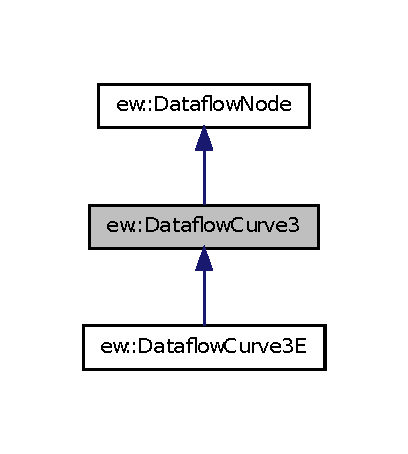
\includegraphics[width=196pt]{classew_1_1DataflowCurve3__inherit__graph}
\end{center}
\end{figure}
\subsubsection*{Public Member Functions}
\begin{DoxyCompactItemize}
\item 
int \hyperlink{classew_1_1DataflowCurve3_afa6639c14717ab3d2a64ed48bc37683d}{get\_\-num\_\-points} () const 
\item 
int \hyperlink{classew_1_1DataflowCurve3_a1617f1c56fc2b04284180f7bb4f707e1}{get\_\-num\_\-edges} () const 
\item 
const float $\ast$ \hyperlink{classew_1_1DataflowCurve3_a8e88c66552e476c51b3719e7316d3565}{get\_\-points} () const 
\item 
const int $\ast$ \hyperlink{classew_1_1DataflowCurve3_af1fc7dfffb82610efedae52e69262daf}{get\_\-edges} () const 
\item 
const \hyperlink{classew_1_1Bbox3}{ew::Bbox3} $\ast$ \hyperlink{classew_1_1DataflowCurve3_a11b0a9f416916cf526988d7a787e61f4}{get\_\-bbox} () const 
\item 
void \hyperlink{classew_1_1DataflowCurve3_a3705ea92d9fc796b4013f1b862607c73}{make\_\-index} () const 
\item 
bool \hyperlink{classew_1_1DataflowCurve3_ae1314c04d06c2b29651bedfd0d68e0bd}{index\_\-is\_\-made} () const 
\item 
double \hyperlink{classew_1_1DataflowCurve3_a914a3fd65c2a397f0fef3ad5e1f67bce}{project} (int $\ast$edge, double $\ast$coeffs, double $\ast$tangent, double $\ast$proj, const double $\ast$inp) const 
\end{DoxyCompactItemize}


\subsubsection{Detailed Description}
\hyperlink{classew_1_1DataflowCurve3}{ew::DataflowCurve3} is the base class for nodes containing piecewise-\/linear curves in $\mathbb{R}^3$.

\hyperlink{classew_1_1DataflowCurve3}{ew::DataflowCurve3} is a class without assignment or comparison. There are private member variables.

For efficient rendering of the same curve in multiple windows, an OpenGL display list is constructed containing the basic curve geometry commands. All windows displaying a given curve must share display lists. 

\subsubsection{Member Function Documentation}
\hypertarget{classew_1_1DataflowCurve3_afa6639c14717ab3d2a64ed48bc37683d}{
\index{ew::DataflowCurve3@{ew::DataflowCurve3}!get\_\-num\_\-points@{get\_\-num\_\-points}}
\index{get\_\-num\_\-points@{get\_\-num\_\-points}!ew::DataflowCurve3@{ew::DataflowCurve3}}
\paragraph[{get\_\-num\_\-points}]{\setlength{\rightskip}{0pt plus 5cm}int ew::DataflowCurve3::get\_\-num\_\-points (
\begin{DoxyParamCaption}
{}
\end{DoxyParamCaption}
) const\hspace{0.3cm}{\ttfamily  \mbox{[}inline\mbox{]}}}\hfill}
\label{classew_1_1DataflowCurve3_afa6639c14717ab3d2a64ed48bc37683d}
This will force the network into an updating phase. \begin{DoxyReturn}{Returns}
The number of points used in the curve. 
\end{DoxyReturn}
\hypertarget{classew_1_1DataflowCurve3_a1617f1c56fc2b04284180f7bb4f707e1}{
\index{ew::DataflowCurve3@{ew::DataflowCurve3}!get\_\-num\_\-edges@{get\_\-num\_\-edges}}
\index{get\_\-num\_\-edges@{get\_\-num\_\-edges}!ew::DataflowCurve3@{ew::DataflowCurve3}}
\paragraph[{get\_\-num\_\-edges}]{\setlength{\rightskip}{0pt plus 5cm}int ew::DataflowCurve3::get\_\-num\_\-edges (
\begin{DoxyParamCaption}
{}
\end{DoxyParamCaption}
) const\hspace{0.3cm}{\ttfamily  \mbox{[}inline\mbox{]}}}\hfill}
\label{classew_1_1DataflowCurve3_a1617f1c56fc2b04284180f7bb4f707e1}
This will force the network into an updating phase. \begin{DoxyReturn}{Returns}
The number of triangular edges in the curve. 
\end{DoxyReturn}
\hypertarget{classew_1_1DataflowCurve3_a8e88c66552e476c51b3719e7316d3565}{
\index{ew::DataflowCurve3@{ew::DataflowCurve3}!get\_\-points@{get\_\-points}}
\index{get\_\-points@{get\_\-points}!ew::DataflowCurve3@{ew::DataflowCurve3}}
\paragraph[{get\_\-points}]{\setlength{\rightskip}{0pt plus 5cm}const float $\ast$ ew::DataflowCurve3::get\_\-points (
\begin{DoxyParamCaption}
{}
\end{DoxyParamCaption}
) const\hspace{0.3cm}{\ttfamily  \mbox{[}inline\mbox{]}}}\hfill}
\label{classew_1_1DataflowCurve3_a8e88c66552e476c51b3719e7316d3565}
This will force the network into an updating phase. The pointer is valid until the node or a dependency of the node is changed. \begin{DoxyReturn}{Returns}
A pointer to the coordinates of the points used in the curve. 
\end{DoxyReturn}
\hypertarget{classew_1_1DataflowCurve3_af1fc7dfffb82610efedae52e69262daf}{
\index{ew::DataflowCurve3@{ew::DataflowCurve3}!get\_\-edges@{get\_\-edges}}
\index{get\_\-edges@{get\_\-edges}!ew::DataflowCurve3@{ew::DataflowCurve3}}
\paragraph[{get\_\-edges}]{\setlength{\rightskip}{0pt plus 5cm}const int $\ast$ ew::DataflowCurve3::get\_\-edges (
\begin{DoxyParamCaption}
{}
\end{DoxyParamCaption}
) const\hspace{0.3cm}{\ttfamily  \mbox{[}inline\mbox{]}}}\hfill}
\label{classew_1_1DataflowCurve3_af1fc7dfffb82610efedae52e69262daf}
This will force the network into an updating phase. The pointer is valid until the node or a dependency of the node is changed. \begin{DoxyReturn}{Returns}
A pointer to the indices of the points used in the curve. 
\end{DoxyReturn}
\hypertarget{classew_1_1DataflowCurve3_a11b0a9f416916cf526988d7a787e61f4}{
\index{ew::DataflowCurve3@{ew::DataflowCurve3}!get\_\-bbox@{get\_\-bbox}}
\index{get\_\-bbox@{get\_\-bbox}!ew::DataflowCurve3@{ew::DataflowCurve3}}
\paragraph[{get\_\-bbox}]{\setlength{\rightskip}{0pt plus 5cm}const {\bf ew::Bbox3} $\ast$ ew::DataflowCurve3::get\_\-bbox (
\begin{DoxyParamCaption}
{}
\end{DoxyParamCaption}
) const\hspace{0.3cm}{\ttfamily  \mbox{[}inline\mbox{]}}}\hfill}
\label{classew_1_1DataflowCurve3_a11b0a9f416916cf526988d7a787e61f4}
The pointer is valid until the node or a dependency of the node is changed. \begin{DoxyReturn}{Returns}
A pointer to the bounding box of the curve. 
\end{DoxyReturn}
\hypertarget{classew_1_1DataflowCurve3_a3705ea92d9fc796b4013f1b862607c73}{
\index{ew::DataflowCurve3@{ew::DataflowCurve3}!make\_\-index@{make\_\-index}}
\index{make\_\-index@{make\_\-index}!ew::DataflowCurve3@{ew::DataflowCurve3}}
\paragraph[{make\_\-index}]{\setlength{\rightskip}{0pt plus 5cm}void ew::DataflowCurve3::make\_\-index (
\begin{DoxyParamCaption}
{}
\end{DoxyParamCaption}
) const\hspace{0.3cm}{\ttfamily  \mbox{[}inline\mbox{]}}}\hfill}
\label{classew_1_1DataflowCurve3_a3705ea92d9fc796b4013f1b862607c73}
This makes the curve spatial index if it has not already been made since the curve was last changed. The spatial index is used by \hyperlink{classew_1_1DataflowCurve3_a914a3fd65c2a397f0fef3ad5e1f67bce}{project}. \hypertarget{classew_1_1DataflowCurve3_ae1314c04d06c2b29651bedfd0d68e0bd}{
\index{ew::DataflowCurve3@{ew::DataflowCurve3}!index\_\-is\_\-made@{index\_\-is\_\-made}}
\index{index\_\-is\_\-made@{index\_\-is\_\-made}!ew::DataflowCurve3@{ew::DataflowCurve3}}
\paragraph[{index\_\-is\_\-made}]{\setlength{\rightskip}{0pt plus 5cm}bool ew::DataflowCurve3::index\_\-is\_\-made (
\begin{DoxyParamCaption}
{}
\end{DoxyParamCaption}
) const\hspace{0.3cm}{\ttfamily  \mbox{[}inline\mbox{]}}}\hfill}
\label{classew_1_1DataflowCurve3_ae1314c04d06c2b29651bedfd0d68e0bd}
\begin{DoxyReturn}{Returns}
{\ttfamily true} if the curve spatial index is up to date. 
\end{DoxyReturn}
\hypertarget{classew_1_1DataflowCurve3_a914a3fd65c2a397f0fef3ad5e1f67bce}{
\index{ew::DataflowCurve3@{ew::DataflowCurve3}!project@{project}}
\index{project@{project}!ew::DataflowCurve3@{ew::DataflowCurve3}}
\paragraph[{project}]{\setlength{\rightskip}{0pt plus 5cm}double ew::DataflowCurve3::project (
\begin{DoxyParamCaption}
\item[{int $\ast$}]{ edge, }
\item[{double $\ast$}]{ coeffs, }
\item[{double $\ast$}]{ tangent, }
\item[{double $\ast$}]{ proj, }
\item[{const double $\ast$}]{ inp}
\end{DoxyParamCaption}
) const}\hfill}
\label{classew_1_1DataflowCurve3_a914a3fd65c2a397f0fef3ad5e1f67bce}
This finds the nearest point on the curve to a given point. The curve spatial index will be made if it has not already been made. 
\begin{DoxyParams}{Parameters}
\item[\mbox{\tt[out]} {\em edge}]The index of the edge of the curve containing the nearest point. \item[\mbox{\tt[out]} {\em coeffs}]The coefficients of the nearest point when expressed as a linear combination of the vertices of the edge. \item[\mbox{\tt[out]} {\em tangent}]The interpolated tangent at the nearest point. If a sensible tangent cannot be calculated, an arbitrary unit vector is returned. \item[\mbox{\tt[out]} {\em proj}]The coordinates of the nearest point on the curve. \item[\mbox{\tt[in]} {\em inp}]The coordinates of the original point. \end{DoxyParams}
\begin{DoxyReturn}{Returns}
The distance from the original point to the projected point. 
\end{DoxyReturn}

\hypertarget{classew_1_1DataflowCurve3E}{
\subsection{ew::DataflowCurve3E Class Reference}
\label{classew_1_1DataflowCurve3E}\index{ew::DataflowCurve3E@{ew::DataflowCurve3E}}
}


Explicit Curve Node.  




{\ttfamily \#include $<$ew/DataflowCurve3E.h$>$}



Inheritance diagram for ew::DataflowCurve3E:
\nopagebreak
\begin{figure}[H]
\begin{center}
\leavevmode
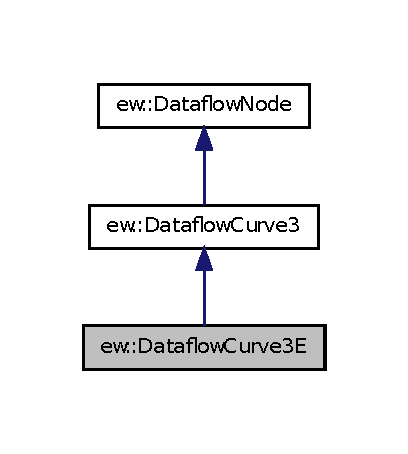
\includegraphics[width=196pt]{classew_1_1DataflowCurve3E__inherit__graph}
\end{center}
\end{figure}
\subsubsection*{Public Member Functions}
\begin{DoxyCompactItemize}
\item 
\hyperlink{classew_1_1DataflowCurve3E_acf5061729d97743dfd2eca60bec86956}{DataflowCurve3E} (\hyperlink{classew_1_1DataflowNetwork}{ew::DataflowNetwork} $\ast$i\_\-network)
\item 
void \hyperlink{classew_1_1DataflowCurve3E_a3e28251e9ceba31390f52e7eb259e463}{set\_\-data} (\hyperlink{classew_1_1Curve3}{ew::Curve3} $\ast$data)
\item 
const \hyperlink{classew_1_1Curve3}{ew::Curve3} $\ast$ \hyperlink{classew_1_1DataflowCurve3E_a6e3cd74e6761953a11fb5a19375abc13}{get\_\-data} () const 
\end{DoxyCompactItemize}


\subsubsection{Detailed Description}
\hyperlink{classew_1_1DataflowCurve3E}{ew::DataflowCurve3E} is a node containing an explicitly specified curve.

\hyperlink{classew_1_1DataflowCurve3E}{ew::DataflowCurve3E} objects may not be copied or compared. There are private member variables.

Nodes of this class do not depend on other nodes, but other nodes can depend on them. They are valid if they have some faces.

Initially and when reset, the node is empty. 

\subsubsection{Constructor \& Destructor Documentation}
\hypertarget{classew_1_1DataflowCurve3E_acf5061729d97743dfd2eca60bec86956}{
\index{ew::DataflowCurve3E@{ew::DataflowCurve3E}!DataflowCurve3E@{DataflowCurve3E}}
\index{DataflowCurve3E@{DataflowCurve3E}!ew::DataflowCurve3E@{ew::DataflowCurve3E}}
\paragraph[{DataflowCurve3E}]{\setlength{\rightskip}{0pt plus 5cm}ew::DataflowCurve3E::DataflowCurve3E (
\begin{DoxyParamCaption}
\item[{{\bf ew::DataflowNetwork} $\ast$}]{ i\_\-network}
\end{DoxyParamCaption}
)\hspace{0.3cm}{\ttfamily  \mbox{[}explicit\mbox{]}}}\hfill}
\label{classew_1_1DataflowCurve3E_acf5061729d97743dfd2eca60bec86956}
This creates an explicit curve node. 
\begin{DoxyParams}{Parameters}
\item[{\em i\_\-network}]The network this node should belong to. \end{DoxyParams}


\subsubsection{Member Function Documentation}
\hypertarget{classew_1_1DataflowCurve3E_a3e28251e9ceba31390f52e7eb259e463}{
\index{ew::DataflowCurve3E@{ew::DataflowCurve3E}!set\_\-data@{set\_\-data}}
\index{set\_\-data@{set\_\-data}!ew::DataflowCurve3E@{ew::DataflowCurve3E}}
\paragraph[{set\_\-data}]{\setlength{\rightskip}{0pt plus 5cm}void ew::DataflowCurve3E::set\_\-data (
\begin{DoxyParamCaption}
\item[{{\bf ew::Curve3} $\ast$}]{ data}
\end{DoxyParamCaption}
)}\hfill}
\label{classew_1_1DataflowCurve3E_a3e28251e9ceba31390f52e7eb259e463}
This transfers the curve data from the \hyperlink{classew_1_1Curve3}{ew::Curve3} object to the node. Afterwards, the \hyperlink{classew_1_1Curve3}{ew::Curve3} object is reset. \begin{DoxyPrecond}{Precondition}
This node must not be a cached node. 
\end{DoxyPrecond}

\begin{DoxyParams}{Parameters}
\item[{\em data}]The object containing the curve data. \end{DoxyParams}
\hypertarget{classew_1_1DataflowCurve3E_a6e3cd74e6761953a11fb5a19375abc13}{
\index{ew::DataflowCurve3E@{ew::DataflowCurve3E}!get\_\-data@{get\_\-data}}
\index{get\_\-data@{get\_\-data}!ew::DataflowCurve3E@{ew::DataflowCurve3E}}
\paragraph[{get\_\-data}]{\setlength{\rightskip}{0pt plus 5cm}const {\bf ew::Curve3} $\ast$ ew::DataflowCurve3E::get\_\-data (
\begin{DoxyParamCaption}
{}
\end{DoxyParamCaption}
) const\hspace{0.3cm}{\ttfamily  \mbox{[}inline\mbox{]}}}\hfill}
\label{classew_1_1DataflowCurve3E_a6e3cd74e6761953a11fb5a19375abc13}
\begin{DoxyReturn}{Returns}
A pointer to the internal curve data. 
\end{DoxyReturn}

\hypertarget{classew_1_1DataflowForm3}{
\subsection{ew::DataflowForm3 Class Reference}
\label{classew_1_1DataflowForm3}\index{ew::DataflowForm3@{ew::DataflowForm3}}
}


3D Form Node  




{\ttfamily \#include $<$ew/DataflowForm3.h$>$}



Inheritance diagram for ew::DataflowForm3:
\nopagebreak
\begin{figure}[H]
\begin{center}
\leavevmode
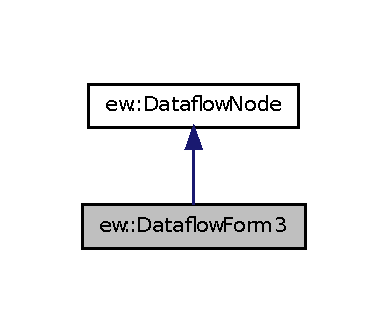
\includegraphics[width=186pt]{classew_1_1DataflowForm3__inherit__graph}
\end{center}
\end{figure}
\subsubsection*{Public Member Functions}
\begin{DoxyCompactItemize}
\item 
\hyperlink{classew_1_1DataflowForm3_aecb15fc6bd28560fa8dafcf6a2cb0ec0}{DataflowForm3} (\hyperlink{classew_1_1DataflowNetwork}{ew::DataflowNetwork} $\ast$i\_\-network)
\item 
void \hyperlink{classew_1_1DataflowForm3_a4efca0bcc9455856e1e5158262804a5e}{set\_\-data} (const \hyperlink{classew_1_1Form3}{ew::Form3} $\ast$data)
\item 
const \hyperlink{classew_1_1Form3}{ew::Form3} $\ast$ \hyperlink{classew_1_1DataflowForm3_a22276b5dc185fec2755c738462d583ce}{get\_\-data} () const 
\item 
int \hyperlink{classew_1_1DataflowForm3_a2b96dfb011fcb937f8663305c99a6559}{set\_\-volume} (bool $\ast$replaced, const \hyperlink{classew_1_1Form3Volume}{ew::Form3Volume} $\ast$vl)
\item 
void \hyperlink{classew_1_1DataflowForm3_a47a6c489b99dac0008982202c49905f1}{remove\_\-volume} (int n)
\item 
int \hyperlink{classew_1_1DataflowForm3_a594e80da7f80db8fc1a7be5ae818002b}{set\_\-surface} (bool $\ast$replaced, const \hyperlink{classew_1_1Form3Surface}{ew::Form3Surface} $\ast$sr)
\item 
void \hyperlink{classew_1_1DataflowForm3_a7ac39098b59bf186401646e5242b6dde}{remove\_\-surface} (int n)
\item 
int \hyperlink{classew_1_1DataflowForm3_ad767440f3efb381c6f19311ae8deb6bd}{set\_\-curve} (bool $\ast$replaced, const \hyperlink{classew_1_1Form3Curve}{ew::Form3Curve} $\ast$cr)
\item 
void \hyperlink{classew_1_1DataflowForm3_a12c6b8481bf7f30a3b83345fc3102247}{remove\_\-curve} (int n)
\item 
int \hyperlink{classew_1_1DataflowForm3_aab8125aabb9eb23fa6292b61b5f39a03}{set\_\-pointset} (bool $\ast$replaced, const \hyperlink{classew_1_1Form3PointSet}{ew::Form3PointSet} $\ast$ps)
\item 
void \hyperlink{classew_1_1DataflowForm3_a5690394f7004a0d8b6799a736c6e485f}{set\_\-pointset\_\-location} (int n, int i, const double $\ast$loc)
\item 
void \hyperlink{classew_1_1DataflowForm3_aec5d6d3b7e412960fcce347ff9dff063}{set\_\-pointset\_\-relax} (int n, int i, int rdim, const double $\ast$rparam)
\item 
void \hyperlink{classew_1_1DataflowForm3_a68f768e333b3bff1bf4d31d57974b160}{remove\_\-pointset} (int n)
\item 
int \hyperlink{classew_1_1DataflowForm3_a20f9365d1235407e6a9ddea3eff6bec3}{set\_\-embedding} (bool $\ast$replaced, const \hyperlink{classew_1_1Form3Embedding}{ew::Form3Embedding} $\ast$em)
\item 
void \hyperlink{classew_1_1DataflowForm3_a59ee4917704ef9d3d912bc48988c6239}{set\_\-superset} (const char $\ast$subset\_\-id, const char $\ast$superset\_\-id)
\item 
void \hyperlink{classew_1_1DataflowForm3_a88961709ad75d7dc70c0e4b9d23eac0c}{remove\_\-embedding} (int n)
\item 
int \hyperlink{classew_1_1DataflowForm3_a0f41241a4d9e418d124c791d77e578e8}{set\_\-reflection} (bool $\ast$replaced, const \hyperlink{classew_1_1Form3Reflection}{ew::Form3Reflection} $\ast$rf)
\item 
void \hyperlink{classew_1_1DataflowForm3_abbb32aecef2237f1901a787d2ec64283}{remove\_\-reflection} (int n)
\item 
unsigned long \hyperlink{classew_1_1DataflowForm3_abcf490e0af0eb5255bde9a0c9aab2805}{get\_\-change\_\-cycle\_\-association} () const 
\item 
unsigned long \hyperlink{classew_1_1DataflowForm3_a681592d654a425f8affadc82bb492e45}{get\_\-change\_\-cycle\_\-coords} () const 
\item 
unsigned long \hyperlink{classew_1_1DataflowForm3_aa05810f772580916a90f388c294811d2}{get\_\-change\_\-cycle\_\-relax} () const 
\item 
const \hyperlink{classew_1_1Bbox3}{ew::Bbox3} $\ast$ \hyperlink{classew_1_1DataflowForm3_aabe57915af91eba8b4c2d254acd4776d}{get\_\-bbox} () const 
\end{DoxyCompactItemize}


\subsubsection{Detailed Description}
\hyperlink{classew_1_1DataflowForm3}{ew::DataflowForm3} is a node that manages an \hyperlink{classew_1_1Form3}{ew::Form3}.

\hyperlink{classew_1_1DataflowForm3}{ew::DataflowForm3} is a class without assignment or comparison. There are private member variables.

Nodes of this class do not depend on other nodes, but other nodes can depend on them. They are always considered valid.

Initially and when reset, the node is empty. 

\subsubsection{Constructor \& Destructor Documentation}
\hypertarget{classew_1_1DataflowForm3_aecb15fc6bd28560fa8dafcf6a2cb0ec0}{
\index{ew::DataflowForm3@{ew::DataflowForm3}!DataflowForm3@{DataflowForm3}}
\index{DataflowForm3@{DataflowForm3}!ew::DataflowForm3@{ew::DataflowForm3}}
\paragraph[{DataflowForm3}]{\setlength{\rightskip}{0pt plus 5cm}ew::DataflowForm3::DataflowForm3 (
\begin{DoxyParamCaption}
\item[{{\bf ew::DataflowNetwork} $\ast$}]{ i\_\-network}
\end{DoxyParamCaption}
)\hspace{0.3cm}{\ttfamily  \mbox{[}explicit\mbox{]}}}\hfill}
\label{classew_1_1DataflowForm3_aecb15fc6bd28560fa8dafcf6a2cb0ec0}
This creates a form3 node. 
\begin{DoxyParams}{Parameters}
\item[{\em i\_\-network}]The network this node should belong to. \end{DoxyParams}


\subsubsection{Member Function Documentation}
\hypertarget{classew_1_1DataflowForm3_a4efca0bcc9455856e1e5158262804a5e}{
\index{ew::DataflowForm3@{ew::DataflowForm3}!set\_\-data@{set\_\-data}}
\index{set\_\-data@{set\_\-data}!ew::DataflowForm3@{ew::DataflowForm3}}
\paragraph[{set\_\-data}]{\setlength{\rightskip}{0pt plus 5cm}void ew::DataflowForm3::set\_\-data (
\begin{DoxyParamCaption}
\item[{const {\bf ew::Form3} $\ast$}]{ data}
\end{DoxyParamCaption}
)}\hfill}
\label{classew_1_1DataflowForm3_a4efca0bcc9455856e1e5158262804a5e}
This sets the contents of the node. 
\begin{DoxyParams}{Parameters}
\item[{\em data}]A pointer to the \hyperlink{classew_1_1Form3}{ew::Form3} data to copy. \end{DoxyParams}
\hypertarget{classew_1_1DataflowForm3_a22276b5dc185fec2755c738462d583ce}{
\index{ew::DataflowForm3@{ew::DataflowForm3}!get\_\-data@{get\_\-data}}
\index{get\_\-data@{get\_\-data}!ew::DataflowForm3@{ew::DataflowForm3}}
\paragraph[{get\_\-data}]{\setlength{\rightskip}{0pt plus 5cm}const {\bf ew::Form3} $\ast$ ew::DataflowForm3::get\_\-data (
\begin{DoxyParamCaption}
{}
\end{DoxyParamCaption}
) const\hspace{0.3cm}{\ttfamily  \mbox{[}inline\mbox{]}}}\hfill}
\label{classew_1_1DataflowForm3_a22276b5dc185fec2755c738462d583ce}
\begin{DoxyReturn}{Returns}
A pointer to the current \hyperlink{classew_1_1Form3}{ew::Form3} data contained in the node. 
\end{DoxyReturn}
\hypertarget{classew_1_1DataflowForm3_a2b96dfb011fcb937f8663305c99a6559}{
\index{ew::DataflowForm3@{ew::DataflowForm3}!set\_\-volume@{set\_\-volume}}
\index{set\_\-volume@{set\_\-volume}!ew::DataflowForm3@{ew::DataflowForm3}}
\paragraph[{set\_\-volume}]{\setlength{\rightskip}{0pt plus 5cm}int ew::DataflowForm3::set\_\-volume (
\begin{DoxyParamCaption}
\item[{bool $\ast$}]{ replaced, }
\item[{const {\bf ew::Form3Volume} $\ast$}]{ vl}
\end{DoxyParamCaption}
)}\hfill}
\label{classew_1_1DataflowForm3_a2b96dfb011fcb937f8663305c99a6559}
This adds or replaces a volume in the \hyperlink{classew_1_1Form3}{ew::Form3} data managed by the node. 
\begin{DoxyParams}{Parameters}
\item[\mbox{\tt[out]} {\em replaced}]{\ttfamily true} if the volume replaced an existing volume. \item[{\em vl}]A pointer to the volume data to copy. \end{DoxyParams}
\begin{DoxyReturn}{Returns}
The index of the new volume in \hyperlink{classew_1_1Form3_aab5dcd7658c84512d05e095e58341fa7}{ew::Form3::volumes}. 
\end{DoxyReturn}
\hypertarget{classew_1_1DataflowForm3_a47a6c489b99dac0008982202c49905f1}{
\index{ew::DataflowForm3@{ew::DataflowForm3}!remove\_\-volume@{remove\_\-volume}}
\index{remove\_\-volume@{remove\_\-volume}!ew::DataflowForm3@{ew::DataflowForm3}}
\paragraph[{remove\_\-volume}]{\setlength{\rightskip}{0pt plus 5cm}void ew::DataflowForm3::remove\_\-volume (
\begin{DoxyParamCaption}
\item[{int}]{ n}
\end{DoxyParamCaption}
)}\hfill}
\label{classew_1_1DataflowForm3_a47a6c489b99dac0008982202c49905f1}
This deletes a volume in the \hyperlink{classew_1_1Form3}{ew::Form3} managed by the node. 
\begin{DoxyParams}{Parameters}
\item[{\em n}]The index of the volume to delete. \end{DoxyParams}
\hypertarget{classew_1_1DataflowForm3_a594e80da7f80db8fc1a7be5ae818002b}{
\index{ew::DataflowForm3@{ew::DataflowForm3}!set\_\-surface@{set\_\-surface}}
\index{set\_\-surface@{set\_\-surface}!ew::DataflowForm3@{ew::DataflowForm3}}
\paragraph[{set\_\-surface}]{\setlength{\rightskip}{0pt plus 5cm}int ew::DataflowForm3::set\_\-surface (
\begin{DoxyParamCaption}
\item[{bool $\ast$}]{ replaced, }
\item[{const {\bf ew::Form3Surface} $\ast$}]{ sr}
\end{DoxyParamCaption}
)}\hfill}
\label{classew_1_1DataflowForm3_a594e80da7f80db8fc1a7be5ae818002b}
This adds or replaces a surface in the \hyperlink{classew_1_1Form3}{ew::Form3} data managed by the node. 
\begin{DoxyParams}{Parameters}
\item[\mbox{\tt[out]} {\em replaced}]{\ttfamily true} if the surface replaced an existing surface. \item[{\em sr}]A pointer to the surface data to copy. \end{DoxyParams}
\begin{DoxyReturn}{Returns}
The index of the new surface in \hyperlink{classew_1_1Form3_abd4405612b484b5d9d87b643d316b020}{ew::Form3::surfaces}. 
\end{DoxyReturn}
\hypertarget{classew_1_1DataflowForm3_a7ac39098b59bf186401646e5242b6dde}{
\index{ew::DataflowForm3@{ew::DataflowForm3}!remove\_\-surface@{remove\_\-surface}}
\index{remove\_\-surface@{remove\_\-surface}!ew::DataflowForm3@{ew::DataflowForm3}}
\paragraph[{remove\_\-surface}]{\setlength{\rightskip}{0pt plus 5cm}void ew::DataflowForm3::remove\_\-surface (
\begin{DoxyParamCaption}
\item[{int}]{ n}
\end{DoxyParamCaption}
)}\hfill}
\label{classew_1_1DataflowForm3_a7ac39098b59bf186401646e5242b6dde}
This deletes a surface in the \hyperlink{classew_1_1Form3}{ew::Form3} managed by the node. 
\begin{DoxyParams}{Parameters}
\item[{\em n}]The index of the surface to delete. \end{DoxyParams}
\hypertarget{classew_1_1DataflowForm3_ad767440f3efb381c6f19311ae8deb6bd}{
\index{ew::DataflowForm3@{ew::DataflowForm3}!set\_\-curve@{set\_\-curve}}
\index{set\_\-curve@{set\_\-curve}!ew::DataflowForm3@{ew::DataflowForm3}}
\paragraph[{set\_\-curve}]{\setlength{\rightskip}{0pt plus 5cm}int ew::DataflowForm3::set\_\-curve (
\begin{DoxyParamCaption}
\item[{bool $\ast$}]{ replaced, }
\item[{const {\bf ew::Form3Curve} $\ast$}]{ cr}
\end{DoxyParamCaption}
)}\hfill}
\label{classew_1_1DataflowForm3_ad767440f3efb381c6f19311ae8deb6bd}
This adds or replaces a curve in the \hyperlink{classew_1_1Form3}{ew::Form3} data managed by the node. 
\begin{DoxyParams}{Parameters}
\item[\mbox{\tt[out]} {\em replaced}]{\ttfamily true} if the curve replaced an existing curve. \item[{\em cr}]A pointer to the curve data to copy. \end{DoxyParams}
\begin{DoxyReturn}{Returns}
The index of the new curve in \hyperlink{classew_1_1Form3_ab60def495fb8fea585dff2fb8c94d845}{ew::Form3::curves}. 
\end{DoxyReturn}
\hypertarget{classew_1_1DataflowForm3_a12c6b8481bf7f30a3b83345fc3102247}{
\index{ew::DataflowForm3@{ew::DataflowForm3}!remove\_\-curve@{remove\_\-curve}}
\index{remove\_\-curve@{remove\_\-curve}!ew::DataflowForm3@{ew::DataflowForm3}}
\paragraph[{remove\_\-curve}]{\setlength{\rightskip}{0pt plus 5cm}void ew::DataflowForm3::remove\_\-curve (
\begin{DoxyParamCaption}
\item[{int}]{ n}
\end{DoxyParamCaption}
)}\hfill}
\label{classew_1_1DataflowForm3_a12c6b8481bf7f30a3b83345fc3102247}
This deletes a curve in the \hyperlink{classew_1_1Form3}{ew::Form3} managed by the node. 
\begin{DoxyParams}{Parameters}
\item[{\em n}]The index of the curve to delete. \end{DoxyParams}
\hypertarget{classew_1_1DataflowForm3_aab8125aabb9eb23fa6292b61b5f39a03}{
\index{ew::DataflowForm3@{ew::DataflowForm3}!set\_\-pointset@{set\_\-pointset}}
\index{set\_\-pointset@{set\_\-pointset}!ew::DataflowForm3@{ew::DataflowForm3}}
\paragraph[{set\_\-pointset}]{\setlength{\rightskip}{0pt plus 5cm}int ew::DataflowForm3::set\_\-pointset (
\begin{DoxyParamCaption}
\item[{bool $\ast$}]{ replaced, }
\item[{const {\bf ew::Form3PointSet} $\ast$}]{ ps}
\end{DoxyParamCaption}
)}\hfill}
\label{classew_1_1DataflowForm3_aab8125aabb9eb23fa6292b61b5f39a03}
This adds or replaces a point set in the \hyperlink{classew_1_1Form3}{ew::Form3} data managed by the node. 
\begin{DoxyParams}{Parameters}
\item[\mbox{\tt[out]} {\em replaced}]{\ttfamily true} if the point set replaced an existing point set. \item[{\em ps}]A pointer to the point set data to copy. \end{DoxyParams}
\begin{DoxyReturn}{Returns}
The index of the new or replaced pointset. 
\end{DoxyReturn}
\hypertarget{classew_1_1DataflowForm3_a5690394f7004a0d8b6799a736c6e485f}{
\index{ew::DataflowForm3@{ew::DataflowForm3}!set\_\-pointset\_\-location@{set\_\-pointset\_\-location}}
\index{set\_\-pointset\_\-location@{set\_\-pointset\_\-location}!ew::DataflowForm3@{ew::DataflowForm3}}
\paragraph[{set\_\-pointset\_\-location}]{\setlength{\rightskip}{0pt plus 5cm}void ew::DataflowForm3::set\_\-pointset\_\-location (
\begin{DoxyParamCaption}
\item[{int}]{ n, }
\item[{int}]{ i, }
\item[{const double $\ast$}]{ loc}
\end{DoxyParamCaption}
)}\hfill}
\label{classew_1_1DataflowForm3_a5690394f7004a0d8b6799a736c6e485f}
This changes the coordinates of an element of the point set. 
\begin{DoxyParams}{Parameters}
\item[{\em n}]The index of the point set. \item[{\em i}]The index of the element in the point set. \item[\mbox{\tt[in]} {\em loc}]A pointer to the new coordinates of this entry. \end{DoxyParams}
\hypertarget{classew_1_1DataflowForm3_aec5d6d3b7e412960fcce347ff9dff063}{
\index{ew::DataflowForm3@{ew::DataflowForm3}!set\_\-pointset\_\-relax@{set\_\-pointset\_\-relax}}
\index{set\_\-pointset\_\-relax@{set\_\-pointset\_\-relax}!ew::DataflowForm3@{ew::DataflowForm3}}
\paragraph[{set\_\-pointset\_\-relax}]{\setlength{\rightskip}{0pt plus 5cm}void ew::DataflowForm3::set\_\-pointset\_\-relax (
\begin{DoxyParamCaption}
\item[{int}]{ n, }
\item[{int}]{ i, }
\item[{int}]{ rdim, }
\item[{const double $\ast$}]{ rparam}
\end{DoxyParamCaption}
)}\hfill}
\label{classew_1_1DataflowForm3_aec5d6d3b7e412960fcce347ff9dff063}
This changes the relaxation parameters of an element of the point set. 
\begin{DoxyParams}{Parameters}
\item[{\em n}]The index of the point set. \item[{\em i}]The index of the element in the point set. \item[\mbox{\tt[in]} {\em rdim}]The new relax\_\-dims of this entry. \item[\mbox{\tt[in]} {\em rparam}]A pointer to the new relax\_\-params of this entry. \end{DoxyParams}
\hypertarget{classew_1_1DataflowForm3_a68f768e333b3bff1bf4d31d57974b160}{
\index{ew::DataflowForm3@{ew::DataflowForm3}!remove\_\-pointset@{remove\_\-pointset}}
\index{remove\_\-pointset@{remove\_\-pointset}!ew::DataflowForm3@{ew::DataflowForm3}}
\paragraph[{remove\_\-pointset}]{\setlength{\rightskip}{0pt plus 5cm}void ew::DataflowForm3::remove\_\-pointset (
\begin{DoxyParamCaption}
\item[{int}]{ n}
\end{DoxyParamCaption}
)}\hfill}
\label{classew_1_1DataflowForm3_a68f768e333b3bff1bf4d31d57974b160}
This deletes a point set in the \hyperlink{classew_1_1Form3}{ew::Form3} managed by the node. 
\begin{DoxyParams}{Parameters}
\item[{\em n}]The index of the point set to delete. \end{DoxyParams}
\hypertarget{classew_1_1DataflowForm3_a20f9365d1235407e6a9ddea3eff6bec3}{
\index{ew::DataflowForm3@{ew::DataflowForm3}!set\_\-embedding@{set\_\-embedding}}
\index{set\_\-embedding@{set\_\-embedding}!ew::DataflowForm3@{ew::DataflowForm3}}
\paragraph[{set\_\-embedding}]{\setlength{\rightskip}{0pt plus 5cm}int ew::DataflowForm3::set\_\-embedding (
\begin{DoxyParamCaption}
\item[{bool $\ast$}]{ replaced, }
\item[{const {\bf ew::Form3Embedding} $\ast$}]{ em}
\end{DoxyParamCaption}
)}\hfill}
\label{classew_1_1DataflowForm3_a20f9365d1235407e6a9ddea3eff6bec3}
This adds or replaces a embedding in the \hyperlink{classew_1_1Form3}{ew::Form3} data managed by the node. 
\begin{DoxyParams}{Parameters}
\item[\mbox{\tt[out]} {\em replaced}]{\ttfamily true} if the embedding replaced an existing embedding. \item[{\em em}]A pointer to the embedding data to copy. \end{DoxyParams}
\begin{DoxyReturn}{Returns}
The index of the new embedding in \hyperlink{classew_1_1Form3_a05ace76e2206ea825495538e93d9ba4c}{ew::Form3::embeddings}. 
\end{DoxyReturn}
\hypertarget{classew_1_1DataflowForm3_a59ee4917704ef9d3d912bc48988c6239}{
\index{ew::DataflowForm3@{ew::DataflowForm3}!set\_\-superset@{set\_\-superset}}
\index{set\_\-superset@{set\_\-superset}!ew::DataflowForm3@{ew::DataflowForm3}}
\paragraph[{set\_\-superset}]{\setlength{\rightskip}{0pt plus 5cm}void ew::DataflowForm3::set\_\-superset (
\begin{DoxyParamCaption}
\item[{const char $\ast$}]{ subset\_\-id, }
\item[{const char $\ast$}]{ superset\_\-id}
\end{DoxyParamCaption}
)}\hfill}
\label{classew_1_1DataflowForm3_a59ee4917704ef9d3d912bc48988c6239}
This makes one element of the form the unique superset of another element. 
\begin{DoxyParams}{Parameters}
\item[{\em subset\_\-id}]The id of the element that should have a unique superset. \item[{\em superset\_\-id}]The id of the element that be the unique superset. \end{DoxyParams}
\hypertarget{classew_1_1DataflowForm3_a88961709ad75d7dc70c0e4b9d23eac0c}{
\index{ew::DataflowForm3@{ew::DataflowForm3}!remove\_\-embedding@{remove\_\-embedding}}
\index{remove\_\-embedding@{remove\_\-embedding}!ew::DataflowForm3@{ew::DataflowForm3}}
\paragraph[{remove\_\-embedding}]{\setlength{\rightskip}{0pt plus 5cm}void ew::DataflowForm3::remove\_\-embedding (
\begin{DoxyParamCaption}
\item[{int}]{ n}
\end{DoxyParamCaption}
)}\hfill}
\label{classew_1_1DataflowForm3_a88961709ad75d7dc70c0e4b9d23eac0c}
This deletes a embedding in the \hyperlink{classew_1_1Form3}{ew::Form3} managed by the node. 
\begin{DoxyParams}{Parameters}
\item[{\em n}]The index of the embedding to delete. \end{DoxyParams}
\hypertarget{classew_1_1DataflowForm3_a0f41241a4d9e418d124c791d77e578e8}{
\index{ew::DataflowForm3@{ew::DataflowForm3}!set\_\-reflection@{set\_\-reflection}}
\index{set\_\-reflection@{set\_\-reflection}!ew::DataflowForm3@{ew::DataflowForm3}}
\paragraph[{set\_\-reflection}]{\setlength{\rightskip}{0pt plus 5cm}int ew::DataflowForm3::set\_\-reflection (
\begin{DoxyParamCaption}
\item[{bool $\ast$}]{ replaced, }
\item[{const {\bf ew::Form3Reflection} $\ast$}]{ rf}
\end{DoxyParamCaption}
)}\hfill}
\label{classew_1_1DataflowForm3_a0f41241a4d9e418d124c791d77e578e8}
This adds or replaces a reflection in the \hyperlink{classew_1_1Form3}{ew::Form3} data managed by the node. 
\begin{DoxyParams}{Parameters}
\item[\mbox{\tt[out]} {\em replaced}]{\ttfamily true} if the reflection replaced an existing reflection. \item[{\em rf}]A pointer to the reflection data to copy. \end{DoxyParams}
\begin{DoxyReturn}{Returns}
The index of the new reflection in \hyperlink{classew_1_1Form3_a4df1d049f2c5ca83f194d4ac9cf9f074}{ew::Form3::reflections}. 
\end{DoxyReturn}
\hypertarget{classew_1_1DataflowForm3_abbb32aecef2237f1901a787d2ec64283}{
\index{ew::DataflowForm3@{ew::DataflowForm3}!remove\_\-reflection@{remove\_\-reflection}}
\index{remove\_\-reflection@{remove\_\-reflection}!ew::DataflowForm3@{ew::DataflowForm3}}
\paragraph[{remove\_\-reflection}]{\setlength{\rightskip}{0pt plus 5cm}void ew::DataflowForm3::remove\_\-reflection (
\begin{DoxyParamCaption}
\item[{int}]{ n}
\end{DoxyParamCaption}
)}\hfill}
\label{classew_1_1DataflowForm3_abbb32aecef2237f1901a787d2ec64283}
This deletes a reflection in the \hyperlink{classew_1_1Form3}{ew::Form3} managed by the node. 
\begin{DoxyParams}{Parameters}
\item[{\em n}]The index of the reflection to delete. \end{DoxyParams}
\hypertarget{classew_1_1DataflowForm3_abcf490e0af0eb5255bde9a0c9aab2805}{
\index{ew::DataflowForm3@{ew::DataflowForm3}!get\_\-change\_\-cycle\_\-association@{get\_\-change\_\-cycle\_\-association}}
\index{get\_\-change\_\-cycle\_\-association@{get\_\-change\_\-cycle\_\-association}!ew::DataflowForm3@{ew::DataflowForm3}}
\paragraph[{get\_\-change\_\-cycle\_\-association}]{\setlength{\rightskip}{0pt plus 5cm}unsigned long ew::DataflowForm3::get\_\-change\_\-cycle\_\-association (
\begin{DoxyParamCaption}
{}
\end{DoxyParamCaption}
) const\hspace{0.3cm}{\ttfamily  \mbox{[}inline\mbox{]}}}\hfill}
\label{classew_1_1DataflowForm3_abcf490e0af0eb5255bde9a0c9aab2805}
\begin{DoxyReturn}{Returns}
The last cycle the form was changed in a way that effects landmark matching. 
\end{DoxyReturn}
\hypertarget{classew_1_1DataflowForm3_a681592d654a425f8affadc82bb492e45}{
\index{ew::DataflowForm3@{ew::DataflowForm3}!get\_\-change\_\-cycle\_\-coords@{get\_\-change\_\-cycle\_\-coords}}
\index{get\_\-change\_\-cycle\_\-coords@{get\_\-change\_\-cycle\_\-coords}!ew::DataflowForm3@{ew::DataflowForm3}}
\paragraph[{get\_\-change\_\-cycle\_\-coords}]{\setlength{\rightskip}{0pt plus 5cm}unsigned long ew::DataflowForm3::get\_\-change\_\-cycle\_\-coords (
\begin{DoxyParamCaption}
{}
\end{DoxyParamCaption}
) const\hspace{0.3cm}{\ttfamily  \mbox{[}inline\mbox{]}}}\hfill}
\label{classew_1_1DataflowForm3_a681592d654a425f8affadc82bb492e45}
\begin{DoxyReturn}{Returns}
The last cycle that any location of a landmark was changed. 
\end{DoxyReturn}
\hypertarget{classew_1_1DataflowForm3_aa05810f772580916a90f388c294811d2}{
\index{ew::DataflowForm3@{ew::DataflowForm3}!get\_\-change\_\-cycle\_\-relax@{get\_\-change\_\-cycle\_\-relax}}
\index{get\_\-change\_\-cycle\_\-relax@{get\_\-change\_\-cycle\_\-relax}!ew::DataflowForm3@{ew::DataflowForm3}}
\paragraph[{get\_\-change\_\-cycle\_\-relax}]{\setlength{\rightskip}{0pt plus 5cm}unsigned long ew::DataflowForm3::get\_\-change\_\-cycle\_\-relax (
\begin{DoxyParamCaption}
{}
\end{DoxyParamCaption}
) const\hspace{0.3cm}{\ttfamily  \mbox{[}inline\mbox{]}}}\hfill}
\label{classew_1_1DataflowForm3_aa05810f772580916a90f388c294811d2}
\begin{DoxyReturn}{Returns}
The last cycle that any relaxation of a landmark was changed. 
\end{DoxyReturn}
\hypertarget{classew_1_1DataflowForm3_aabe57915af91eba8b4c2d254acd4776d}{
\index{ew::DataflowForm3@{ew::DataflowForm3}!get\_\-bbox@{get\_\-bbox}}
\index{get\_\-bbox@{get\_\-bbox}!ew::DataflowForm3@{ew::DataflowForm3}}
\paragraph[{get\_\-bbox}]{\setlength{\rightskip}{0pt plus 5cm}const {\bf ew::Bbox3} $\ast$ ew::DataflowForm3::get\_\-bbox (
\begin{DoxyParamCaption}
{}
\end{DoxyParamCaption}
) const\hspace{0.3cm}{\ttfamily  \mbox{[}inline\mbox{]}}}\hfill}
\label{classew_1_1DataflowForm3_aabe57915af91eba8b4c2d254acd4776d}
The pointer until the node or a dependency of the node is changed. \begin{DoxyReturn}{Returns}
A pointer to the bounding box of the points in the form. 
\end{DoxyReturn}

\hypertarget{classew_1_1DataflowNetwork}{
\subsection{ew::DataflowNetwork Class Reference}
\label{classew_1_1DataflowNetwork}\index{ew::DataflowNetwork@{ew::DataflowNetwork}}
}


Lightweight Dataflow Network.  




{\ttfamily \#include $<$ew/DataflowNetwork.h$>$}

\subsubsection*{Public Member Functions}
\begin{DoxyCompactItemize}
\item 
\hyperlink{classew_1_1DataflowNetwork_ab242538a954258848964351243fb8dd2}{DataflowNetwork} ()
\item 
\hyperlink{classew_1_1DataflowNetwork_afd33505274dcba0faee9a66d07af8f7c}{$\sim$DataflowNetwork} ()
\item 
unsigned long \hyperlink{classew_1_1DataflowNetwork_a07f32aa66b2ba19b133478d6f4ef29df}{get\_\-cycle} () const 
\item 
const \hyperlink{classew_1_1DataflowCurve3E}{ew::DataflowCurve3E} $\ast$ \hyperlink{classew_1_1DataflowNetwork_a584fb4f8718ba69bd97e7f50682a1096}{cached\_\-curve} (const char $\ast$filename)
\item 
const \hyperlink{classew_1_1DataflowSurface3E}{ew::DataflowSurface3E} $\ast$ \hyperlink{classew_1_1DataflowNetwork_a596c51c6fc7684ee5bc5147ba5eaf3f5}{cached\_\-surface} (const char $\ast$filename)
\end{DoxyCompactItemize}


\subsubsection{Detailed Description}
EW::DataflowNetwork provides the infrastructure for a lightweight dataflow network.

To keep track of what calculations done by nodes in the network are up to date, and which need to be redone, EW::DataflowNetwork keeps a cycle counter. A cycle consists of an initial phase, when changes are made to nodes of the network, followed by a second phase, when updates of various calculations are made. Requesting updated output from a node puts the network into the update phase of the same cycle, if it is not already in an update phase. Changing a node puts the network into the change phase of the next cycle, if it is not already in a change phase. Initially the network is in the change phase of cycle 1.

Operations on a network must not be performed simultaneously in different threads. However, operations on different networks may be.

This class does not support assignment or comparison. It contains private members and undocumented members. 

\subsubsection{Constructor \& Destructor Documentation}
\hypertarget{classew_1_1DataflowNetwork_ab242538a954258848964351243fb8dd2}{
\index{ew::DataflowNetwork@{ew::DataflowNetwork}!DataflowNetwork@{DataflowNetwork}}
\index{DataflowNetwork@{DataflowNetwork}!ew::DataflowNetwork@{ew::DataflowNetwork}}
\paragraph[{DataflowNetwork}]{\setlength{\rightskip}{0pt plus 5cm}ew::DataflowNetwork::DataflowNetwork (
\begin{DoxyParamCaption}
{}
\end{DoxyParamCaption}
)}\hfill}
\label{classew_1_1DataflowNetwork_ab242538a954258848964351243fb8dd2}
This creates an empty network. \hypertarget{classew_1_1DataflowNetwork_afd33505274dcba0faee9a66d07af8f7c}{
\index{ew::DataflowNetwork@{ew::DataflowNetwork}!$\sim$DataflowNetwork@{$\sim$DataflowNetwork}}
\index{$\sim$DataflowNetwork@{$\sim$DataflowNetwork}!ew::DataflowNetwork@{ew::DataflowNetwork}}
\paragraph[{$\sim$DataflowNetwork}]{\setlength{\rightskip}{0pt plus 5cm}ew::DataflowNetwork::$\sim$DataflowNetwork (
\begin{DoxyParamCaption}
{}
\end{DoxyParamCaption}
)}\hfill}
\label{classew_1_1DataflowNetwork_afd33505274dcba0faee9a66d07af8f7c}
This destroys the network. All nodes and other objects using this network must already have been destroyed. 

\subsubsection{Member Function Documentation}
\hypertarget{classew_1_1DataflowNetwork_a07f32aa66b2ba19b133478d6f4ef29df}{
\index{ew::DataflowNetwork@{ew::DataflowNetwork}!get\_\-cycle@{get\_\-cycle}}
\index{get\_\-cycle@{get\_\-cycle}!ew::DataflowNetwork@{ew::DataflowNetwork}}
\paragraph[{get\_\-cycle}]{\setlength{\rightskip}{0pt plus 5cm}unsigned long ew::DataflowNetwork::get\_\-cycle (
\begin{DoxyParamCaption}
{}
\end{DoxyParamCaption}
) const\hspace{0.3cm}{\ttfamily  \mbox{[}inline\mbox{]}}}\hfill}
\label{classew_1_1DataflowNetwork_a07f32aa66b2ba19b133478d6f4ef29df}
\begin{DoxyReturn}{Returns}
The current cycle number. 
\end{DoxyReturn}
\hypertarget{classew_1_1DataflowNetwork_a584fb4f8718ba69bd97e7f50682a1096}{
\index{ew::DataflowNetwork@{ew::DataflowNetwork}!cached\_\-curve@{cached\_\-curve}}
\index{cached\_\-curve@{cached\_\-curve}!ew::DataflowNetwork@{ew::DataflowNetwork}}
\paragraph[{cached\_\-curve}]{\setlength{\rightskip}{0pt plus 5cm}const {\bf ew::DataflowCurve3E} $\ast$ ew::DataflowNetwork::cached\_\-curve (
\begin{DoxyParamCaption}
\item[{const char $\ast$}]{ filename}
\end{DoxyParamCaption}
)}\hfill}
\label{classew_1_1DataflowNetwork_a584fb4f8718ba69bd97e7f50682a1096}
The first time this is called with a given filename, it reads the curve from the file, creates a new explicit curve node using it, and returns a pointer to it. Subsequently it increments the same node's reference count and returns a pointer to it. When the pointer to the node is no longer needed, the reference should be released with EW::DataflowNode::decr\_\-ref\_\-count. The cache retains a reference to the node, so it will not be deleted until all other references are released and the network is destroyed. 
\begin{DoxyParams}{Parameters}
\item[{\em filename}]is the canonical name of the file to read. \end{DoxyParams}

\begin{DoxyExceptions}{Exceptions}
\item[{\em std::bad\_\-alloc}]\item[{\em EW::ErrorIO}]\end{DoxyExceptions}
\hypertarget{classew_1_1DataflowNetwork_a596c51c6fc7684ee5bc5147ba5eaf3f5}{
\index{ew::DataflowNetwork@{ew::DataflowNetwork}!cached\_\-surface@{cached\_\-surface}}
\index{cached\_\-surface@{cached\_\-surface}!ew::DataflowNetwork@{ew::DataflowNetwork}}
\paragraph[{cached\_\-surface}]{\setlength{\rightskip}{0pt plus 5cm}const {\bf ew::DataflowSurface3E} $\ast$ ew::DataflowNetwork::cached\_\-surface (
\begin{DoxyParamCaption}
\item[{const char $\ast$}]{ filename}
\end{DoxyParamCaption}
)}\hfill}
\label{classew_1_1DataflowNetwork_a596c51c6fc7684ee5bc5147ba5eaf3f5}
The first time this is called with a given filename, it reads the surface from the file, creates a new explicit surface node using it, and returns a pointer to it. Subsequently it increments the same node's reference count and returns a pointer to it. When the pointer to the node is no longer needed, the reference should be released with EW::DataflowNode::decr\_\-ref\_\-count. The cache retains a reference to the node, so it will not be deleted until all other references are released and the network is destroyed. 
\begin{DoxyParams}{Parameters}
\item[{\em filename}]The name of the file to read. \end{DoxyParams}

\begin{DoxyExceptions}{Exceptions}
\item[{\em std::bad\_\-alloc}]\item[{\em EW::ErrorIO}]\end{DoxyExceptions}

\hypertarget{classew_1_1DataflowNode}{
\subsection{ew::DataflowNode Class Reference}
\label{classew_1_1DataflowNode}\index{ew::DataflowNode@{ew::DataflowNode}}
}


Node Base Class.  




{\ttfamily \#include $<$ew/DataflowNode.h$>$}



Inheritance diagram for ew::DataflowNode:
\nopagebreak
\begin{figure}[H]
\begin{center}
\leavevmode
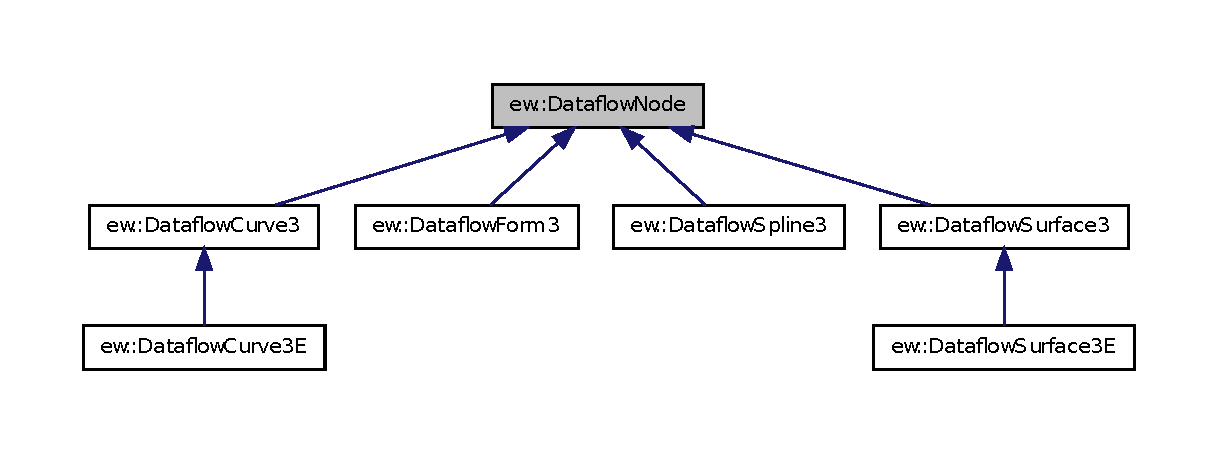
\includegraphics[width=400pt]{classew_1_1DataflowNode__inherit__graph}
\end{center}
\end{figure}
\subsubsection*{Public Member Functions}
\begin{DoxyCompactItemize}
\item 
virtual void \hyperlink{classew_1_1DataflowNode_afb722a0a8129fb026e9ab82c638dda54}{reset} ()=0
\item 
void \hyperlink{classew_1_1DataflowNode_a412a930ede1955b09dcc708dd78469a5}{incr\_\-ref\_\-count} () const 
\item 
void \hyperlink{classew_1_1DataflowNode_a7ee43d6c11ea87911ce0dbc16df0722a}{decr\_\-ref\_\-count} () const 
\item 
unsigned long \hyperlink{classew_1_1DataflowNode_a80553efd99a2247c70b179600cc84fc5}{get\_\-change\_\-cycle} () const 
\item 
unsigned long \hyperlink{classew_1_1DataflowNode_a748037041473e788688117cd99b095c2}{get\_\-version} () const 
\item 
bool \hyperlink{classew_1_1DataflowNode_ab107e9b827f2ce8e9875fff5f90723b0}{get\_\-valid} () const 
\end{DoxyCompactItemize}
\subsubsection*{Public Attributes}
\begin{DoxyCompactItemize}
\item 
\hyperlink{classew_1_1DataflowNetwork}{ew::DataflowNetwork} $\ast$const \hyperlink{classew_1_1DataflowNode_af3e8a9a18dac03806dda98ed1fcc79e9}{network}
\end{DoxyCompactItemize}


\subsubsection{Detailed Description}
EW::DataflowNode is the base class for nodes in a EW::DataflowNetwork.

EW::DataflowNode does not support assignment or comparison. It contains private members, protected members and undocumented members.

Nodes are referenced counted and can only be deleted indirectly by calling \hyperlink{classew_1_1DataflowNode_a7ee43d6c11ea87911ce0dbc16df0722a}{decr\_\-ref\_\-count}. The reference count is set to 1 by the constructor.

Depending on its parameters, a node is considered valid or invalid. What constitutes a valid state depends on the specific node class.

A node can depend on other nodes. The possible dependencies are defined by the specific node class. It is a precondition of methods that set these dependencies that they do not create dependency loops.

After the EW::DataflowNetwork has been destroyed, the only EW::DataflowNode method that may be called is decr\_\-ref\_\-count. 

\subsubsection{Member Function Documentation}
\hypertarget{classew_1_1DataflowNode_afb722a0a8129fb026e9ab82c638dda54}{
\index{ew::DataflowNode@{ew::DataflowNode}!reset@{reset}}
\index{reset@{reset}!ew::DataflowNode@{ew::DataflowNode}}
\paragraph[{reset}]{\setlength{\rightskip}{0pt plus 5cm}virtual void ew::DataflowNode::reset (
\begin{DoxyParamCaption}
{}
\end{DoxyParamCaption}
)\hspace{0.3cm}{\ttfamily  \mbox{[}pure virtual\mbox{]}}}\hfill}
\label{classew_1_1DataflowNode_afb722a0a8129fb026e9ab82c638dda54}
This resets a node to the state it had immediately after construction. \hypertarget{classew_1_1DataflowNode_a412a930ede1955b09dcc708dd78469a5}{
\index{ew::DataflowNode@{ew::DataflowNode}!incr\_\-ref\_\-count@{incr\_\-ref\_\-count}}
\index{incr\_\-ref\_\-count@{incr\_\-ref\_\-count}!ew::DataflowNode@{ew::DataflowNode}}
\paragraph[{incr\_\-ref\_\-count}]{\setlength{\rightskip}{0pt plus 5cm}void ew::DataflowNode::incr\_\-ref\_\-count (
\begin{DoxyParamCaption}
{}
\end{DoxyParamCaption}
) const}\hfill}
\label{classew_1_1DataflowNode_a412a930ede1955b09dcc708dd78469a5}
This increases the reference count. \hypertarget{classew_1_1DataflowNode_a7ee43d6c11ea87911ce0dbc16df0722a}{
\index{ew::DataflowNode@{ew::DataflowNode}!decr\_\-ref\_\-count@{decr\_\-ref\_\-count}}
\index{decr\_\-ref\_\-count@{decr\_\-ref\_\-count}!ew::DataflowNode@{ew::DataflowNode}}
\paragraph[{decr\_\-ref\_\-count}]{\setlength{\rightskip}{0pt plus 5cm}void ew::DataflowNode::decr\_\-ref\_\-count (
\begin{DoxyParamCaption}
{}
\end{DoxyParamCaption}
) const}\hfill}
\label{classew_1_1DataflowNode_a7ee43d6c11ea87911ce0dbc16df0722a}
This decreases the reference count. If the reference count becomes zero, the node is deleted. \hypertarget{classew_1_1DataflowNode_a80553efd99a2247c70b179600cc84fc5}{
\index{ew::DataflowNode@{ew::DataflowNode}!get\_\-change\_\-cycle@{get\_\-change\_\-cycle}}
\index{get\_\-change\_\-cycle@{get\_\-change\_\-cycle}!ew::DataflowNode@{ew::DataflowNode}}
\paragraph[{get\_\-change\_\-cycle}]{\setlength{\rightskip}{0pt plus 5cm}unsigned long ew::DataflowNode::get\_\-change\_\-cycle (
\begin{DoxyParamCaption}
{}
\end{DoxyParamCaption}
) const\hspace{0.3cm}{\ttfamily  \mbox{[}inline\mbox{]}}}\hfill}
\label{classew_1_1DataflowNode_a80553efd99a2247c70b179600cc84fc5}
\begin{DoxyReturn}{Returns}
{\ttfamily The} last cycle on which a change to the node was made. 
\end{DoxyReturn}
\hypertarget{classew_1_1DataflowNode_a748037041473e788688117cd99b095c2}{
\index{ew::DataflowNode@{ew::DataflowNode}!get\_\-version@{get\_\-version}}
\index{get\_\-version@{get\_\-version}!ew::DataflowNode@{ew::DataflowNode}}
\paragraph[{get\_\-version}]{\setlength{\rightskip}{0pt plus 5cm}unsigned long ew::DataflowNode::get\_\-version (
\begin{DoxyParamCaption}
{}
\end{DoxyParamCaption}
) const\hspace{0.3cm}{\ttfamily  \mbox{[}inline\mbox{]}}}\hfill}
\label{classew_1_1DataflowNode_a748037041473e788688117cd99b095c2}
The version of a node is the greater of the last network cycle that any parameter of the node was changed, and the versions of any nodes that the node depends on. This will force the network into an updating phase. \begin{DoxyReturn}{Returns}
{\ttfamily The} version of the node. 
\end{DoxyReturn}
\hypertarget{classew_1_1DataflowNode_ab107e9b827f2ce8e9875fff5f90723b0}{
\index{ew::DataflowNode@{ew::DataflowNode}!get\_\-valid@{get\_\-valid}}
\index{get\_\-valid@{get\_\-valid}!ew::DataflowNode@{ew::DataflowNode}}
\paragraph[{get\_\-valid}]{\setlength{\rightskip}{0pt plus 5cm}bool ew::DataflowNode::get\_\-valid (
\begin{DoxyParamCaption}
{}
\end{DoxyParamCaption}
) const\hspace{0.3cm}{\ttfamily  \mbox{[}inline\mbox{]}}}\hfill}
\label{classew_1_1DataflowNode_ab107e9b827f2ce8e9875fff5f90723b0}
\begin{DoxyReturn}{Returns}
{\ttfamily true} if the node is in a valid state. 
\end{DoxyReturn}
\begin{DoxyPostcond}{Postcondition}
The network will be in an update phase. 
\end{DoxyPostcond}


\subsubsection{Member Data Documentation}
\hypertarget{classew_1_1DataflowNode_af3e8a9a18dac03806dda98ed1fcc79e9}{
\index{ew::DataflowNode@{ew::DataflowNode}!network@{network}}
\index{network@{network}!ew::DataflowNode@{ew::DataflowNode}}
\paragraph[{network}]{\setlength{\rightskip}{0pt plus 5cm}{\bf ew::DataflowNetwork}$\ast$ const {\bf ew::DataflowNode::network}}\hfill}
\label{classew_1_1DataflowNode_af3e8a9a18dac03806dda98ed1fcc79e9}
This points to the EW::Dataflow\_\-Network that this EW::Dataflow\_\-Node was created with. 
\hypertarget{classew_1_1DataflowSpline3}{
\subsection{ew::DataflowSpline3 Class Reference}
\label{classew_1_1DataflowSpline3}\index{ew::DataflowSpline3@{ew::DataflowSpline3}}
}


3D Spline Node  




{\ttfamily \#include $<$ew/DataflowSpline3.h$>$}



Inheritance diagram for ew::DataflowSpline3:
\nopagebreak
\begin{figure}[H]
\begin{center}
\leavevmode
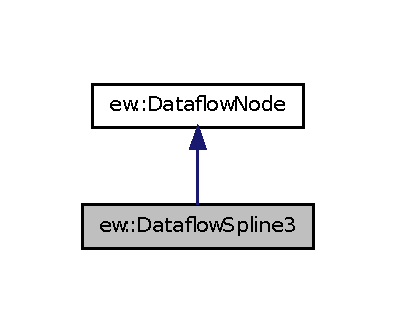
\includegraphics[width=190pt]{classew_1_1DataflowSpline3__inherit__graph}
\end{center}
\end{figure}
\subsubsection*{Public Member Functions}
\begin{DoxyCompactItemize}
\item 
void \hyperlink{classew_1_1DataflowSpline3_a568e3304e82c3659bf60db90857cdbb3}{set\_\-template} (const \hyperlink{classew_1_1DataflowForm3}{ew::DataflowForm3} $\ast$f)
\item 
const \hyperlink{classew_1_1DataflowForm3}{ew::DataflowForm3} $\ast$ \hyperlink{classew_1_1DataflowSpline3_a539e7fc0d4121a31b383a766c243cea7}{get\_\-template} () const 
\item 
unsigned long \hyperlink{classew_1_1DataflowSpline3_af99ac5e26b81ddc18d09713d7ebdc00d}{get\_\-change\_\-cycle\_\-template} () const 
\item 
void \hyperlink{classew_1_1DataflowSpline3_a08c3a3fb2c36969894afa0256282f76c}{set\_\-specimen} (const \hyperlink{classew_1_1DataflowForm3}{ew::DataflowForm3} $\ast$f)
\item 
const \hyperlink{classew_1_1DataflowForm3}{ew::DataflowForm3} $\ast$ \hyperlink{classew_1_1DataflowSpline3_ad0463444434aed2f1b54f7ce16f493bd}{get\_\-specimen} () const 
\item 
unsigned long \hyperlink{classew_1_1DataflowSpline3_a14e8361646fc5fe098b670690038f10b}{get\_\-change\_\-cycle\_\-specimen} () const 
\item 
int \hyperlink{classew_1_1DataflowSpline3_afddea45da34e52c9f28582a1ccca07dd}{get\_\-n\_\-lmks} () const 
\item 
int \hyperlink{classew_1_1DataflowSpline3_aedeb4a2beed67c9ac49caf7300dcd9c5}{get\_\-f\_\-size} () const 
\item 
int \hyperlink{classew_1_1DataflowSpline3_a812346e97afeae66fe6cf9d462fb771a}{lmk\_\-index} (int side, int point\_\-set, int i) const 
\item 
int \hyperlink{classew_1_1DataflowSpline3_aa0a156725d9a29c9d278a2bb90d27d27}{lmk\_\-pointset} (int side, int lmk\_\-index) const 
\item 
int \hyperlink{classew_1_1DataflowSpline3_a49e2ffd2c78efb144d023da9f25d24ca}{lmk\_\-pointset\_\-i} (int side, int lmk\_\-index) const 
\item 
bool \hyperlink{classew_1_1DataflowSpline3_a546e8bf4ffd0f57d04df17a3ffeb8a4c}{get\_\-nonsingular} () const 
\item 
double \hyperlink{classew_1_1DataflowSpline3_a3da92ed8913113804b8d45a60894549b}{get\_\-energy} () const 
\item 
const double $\ast$ \hyperlink{classew_1_1DataflowSpline3_a7597bf0db3a9f8f861dfe5b76a4415fc}{get\_\-optimized\_\-lmk\_\-images} () const 
\item 
void \hyperlink{classew_1_1DataflowSpline3_a8624ee7efc3543e6457a28e05919c3dd}{warp\_\-points} (double $\ast$outp, const double $\ast$inp, int l) const 
\end{DoxyCompactItemize}
\subsubsection*{Private Member Functions}
\begin{DoxyCompactItemize}
\item 
unsigned long \hyperlink{classew_1_1DataflowSpline3_a97c2c2e0955273f4db1cccc052ecfd4a}{get\_\-version\_\-association} () const 
\item 
unsigned long \hyperlink{classew_1_1DataflowSpline3_a7c2c1abc16855dd21e95029e49040ad0}{get\_\-version\_\-interaction} () const 
\item 
unsigned long \hyperlink{classew_1_1DataflowSpline3_afa1dfc18ee811369951af160fd666f81}{get\_\-version\_\-factorization} () const 
\item 
unsigned long \hyperlink{classew_1_1DataflowSpline3_a1db766446fc6eb08ec1a78e8693b45fb}{get\_\-version\_\-spline} () const 
\end{DoxyCompactItemize}


\subsubsection{Detailed Description}
\hyperlink{classew_1_1DataflowSpline3}{ew::DataflowSpline3} is a node that manages a thin-\/plate spline.

\hyperlink{classew_1_1DataflowSpline3}{ew::DataflowSpline3} is a class without assignment or comparison. There are private member variables.

Nodes of this class depend on 2 nodes, the template and specimen \hyperlink{classew_1_1DataflowForm3}{ew::DataflowForm3} nodes. Nodes representing warped geometric objects will depend on a \hyperlink{classew_1_1DataflowSpline3}{ew::DataflowSpline3} node. A ew::Dataflow\_\-Spline3 is considered valid if it's template and specimen dependencies have been set and if there are 4 or more associated landmarks.

Initially and when reset, the node has neither template or specimen set. 

\subsubsection{Member Function Documentation}
\hypertarget{classew_1_1DataflowSpline3_a568e3304e82c3659bf60db90857cdbb3}{
\index{ew::DataflowSpline3@{ew::DataflowSpline3}!set\_\-template@{set\_\-template}}
\index{set\_\-template@{set\_\-template}!ew::DataflowSpline3@{ew::DataflowSpline3}}
\paragraph[{set\_\-template}]{\setlength{\rightskip}{0pt plus 5cm}void ew::DataflowSpline3::set\_\-template (
\begin{DoxyParamCaption}
\item[{const {\bf ew::DataflowForm3} $\ast$}]{ f}
\end{DoxyParamCaption}
)}\hfill}
\label{classew_1_1DataflowSpline3_a568e3304e82c3659bf60db90857cdbb3}

\begin{DoxyParams}{Parameters}
\item[{\em f}]A pointer to the new template form node. \end{DoxyParams}
\hypertarget{classew_1_1DataflowSpline3_a539e7fc0d4121a31b383a766c243cea7}{
\index{ew::DataflowSpline3@{ew::DataflowSpline3}!get\_\-template@{get\_\-template}}
\index{get\_\-template@{get\_\-template}!ew::DataflowSpline3@{ew::DataflowSpline3}}
\paragraph[{get\_\-template}]{\setlength{\rightskip}{0pt plus 5cm}const {\bf ew::DataflowForm3} $\ast$ ew::DataflowSpline3::get\_\-template (
\begin{DoxyParamCaption}
{}
\end{DoxyParamCaption}
) const\hspace{0.3cm}{\ttfamily  \mbox{[}inline\mbox{]}}}\hfill}
\label{classew_1_1DataflowSpline3_a539e7fc0d4121a31b383a766c243cea7}
\begin{DoxyReturn}{Returns}
A pointer to the template node. 
\end{DoxyReturn}
\hypertarget{classew_1_1DataflowSpline3_af99ac5e26b81ddc18d09713d7ebdc00d}{
\index{ew::DataflowSpline3@{ew::DataflowSpline3}!get\_\-change\_\-cycle\_\-template@{get\_\-change\_\-cycle\_\-template}}
\index{get\_\-change\_\-cycle\_\-template@{get\_\-change\_\-cycle\_\-template}!ew::DataflowSpline3@{ew::DataflowSpline3}}
\paragraph[{get\_\-change\_\-cycle\_\-template}]{\setlength{\rightskip}{0pt plus 5cm}unsigned long ew::DataflowSpline3::get\_\-change\_\-cycle\_\-template (
\begin{DoxyParamCaption}
{}
\end{DoxyParamCaption}
) const\hspace{0.3cm}{\ttfamily  \mbox{[}inline\mbox{]}}}\hfill}
\label{classew_1_1DataflowSpline3_af99ac5e26b81ddc18d09713d7ebdc00d}
\begin{DoxyReturn}{Returns}
The last cycle the template pointer was changed. 
\end{DoxyReturn}
\hypertarget{classew_1_1DataflowSpline3_a08c3a3fb2c36969894afa0256282f76c}{
\index{ew::DataflowSpline3@{ew::DataflowSpline3}!set\_\-specimen@{set\_\-specimen}}
\index{set\_\-specimen@{set\_\-specimen}!ew::DataflowSpline3@{ew::DataflowSpline3}}
\paragraph[{set\_\-specimen}]{\setlength{\rightskip}{0pt plus 5cm}void ew::DataflowSpline3::set\_\-specimen (
\begin{DoxyParamCaption}
\item[{const {\bf ew::DataflowForm3} $\ast$}]{ f}
\end{DoxyParamCaption}
)}\hfill}
\label{classew_1_1DataflowSpline3_a08c3a3fb2c36969894afa0256282f76c}

\begin{DoxyParams}{Parameters}
\item[{\em f}]A pointer to the new specimen form node. \end{DoxyParams}
\hypertarget{classew_1_1DataflowSpline3_ad0463444434aed2f1b54f7ce16f493bd}{
\index{ew::DataflowSpline3@{ew::DataflowSpline3}!get\_\-specimen@{get\_\-specimen}}
\index{get\_\-specimen@{get\_\-specimen}!ew::DataflowSpline3@{ew::DataflowSpline3}}
\paragraph[{get\_\-specimen}]{\setlength{\rightskip}{0pt plus 5cm}const {\bf ew::DataflowForm3} $\ast$ ew::DataflowSpline3::get\_\-specimen (
\begin{DoxyParamCaption}
{}
\end{DoxyParamCaption}
) const\hspace{0.3cm}{\ttfamily  \mbox{[}inline\mbox{]}}}\hfill}
\label{classew_1_1DataflowSpline3_ad0463444434aed2f1b54f7ce16f493bd}
\begin{DoxyReturn}{Returns}
A pointer to the specimen node. 
\end{DoxyReturn}
\hypertarget{classew_1_1DataflowSpline3_a14e8361646fc5fe098b670690038f10b}{
\index{ew::DataflowSpline3@{ew::DataflowSpline3}!get\_\-change\_\-cycle\_\-specimen@{get\_\-change\_\-cycle\_\-specimen}}
\index{get\_\-change\_\-cycle\_\-specimen@{get\_\-change\_\-cycle\_\-specimen}!ew::DataflowSpline3@{ew::DataflowSpline3}}
\paragraph[{get\_\-change\_\-cycle\_\-specimen}]{\setlength{\rightskip}{0pt plus 5cm}unsigned long ew::DataflowSpline3::get\_\-change\_\-cycle\_\-specimen (
\begin{DoxyParamCaption}
{}
\end{DoxyParamCaption}
) const\hspace{0.3cm}{\ttfamily  \mbox{[}inline\mbox{]}}}\hfill}
\label{classew_1_1DataflowSpline3_a14e8361646fc5fe098b670690038f10b}
\begin{DoxyReturn}{Returns}
The last cycle the specimen pointer was changed. 
\end{DoxyReturn}
\hypertarget{classew_1_1DataflowSpline3_afddea45da34e52c9f28582a1ccca07dd}{
\index{ew::DataflowSpline3@{ew::DataflowSpline3}!get\_\-n\_\-lmks@{get\_\-n\_\-lmks}}
\index{get\_\-n\_\-lmks@{get\_\-n\_\-lmks}!ew::DataflowSpline3@{ew::DataflowSpline3}}
\paragraph[{get\_\-n\_\-lmks}]{\setlength{\rightskip}{0pt plus 5cm}int ew::DataflowSpline3::get\_\-n\_\-lmks (
\begin{DoxyParamCaption}
{}
\end{DoxyParamCaption}
) const\hspace{0.3cm}{\ttfamily  \mbox{[}inline\mbox{]}}}\hfill}
\label{classew_1_1DataflowSpline3_afddea45da34e52c9f28582a1ccca07dd}
\begin{DoxyReturn}{Returns}
The number of landmarks and semi-\/landmarks matched between template and specimen. 
\end{DoxyReturn}
\hypertarget{classew_1_1DataflowSpline3_aedeb4a2beed67c9ac49caf7300dcd9c5}{
\index{ew::DataflowSpline3@{ew::DataflowSpline3}!get\_\-f\_\-size@{get\_\-f\_\-size}}
\index{get\_\-f\_\-size@{get\_\-f\_\-size}!ew::DataflowSpline3@{ew::DataflowSpline3}}
\paragraph[{get\_\-f\_\-size}]{\setlength{\rightskip}{0pt plus 5cm}int ew::DataflowSpline3::get\_\-f\_\-size (
\begin{DoxyParamCaption}
{}
\end{DoxyParamCaption}
) const\hspace{0.3cm}{\ttfamily  \mbox{[}inline\mbox{]}}}\hfill}
\label{classew_1_1DataflowSpline3_aedeb4a2beed67c9ac49caf7300dcd9c5}
\begin{DoxyReturn}{Returns}
The algebraic dimension of the spline, or -\/1. 
\end{DoxyReturn}
\hypertarget{classew_1_1DataflowSpline3_a812346e97afeae66fe6cf9d462fb771a}{
\index{ew::DataflowSpline3@{ew::DataflowSpline3}!lmk\_\-index@{lmk\_\-index}}
\index{lmk\_\-index@{lmk\_\-index}!ew::DataflowSpline3@{ew::DataflowSpline3}}
\paragraph[{lmk\_\-index}]{\setlength{\rightskip}{0pt plus 5cm}int ew::DataflowSpline3::lmk\_\-index (
\begin{DoxyParamCaption}
\item[{int}]{ side, }
\item[{int}]{ point\_\-set, }
\item[{int}]{ i}
\end{DoxyParamCaption}
) const\hspace{0.3cm}{\ttfamily  \mbox{[}inline\mbox{]}}}\hfill}
\label{classew_1_1DataflowSpline3_a812346e97afeae66fe6cf9d462fb771a}
To construct the spline, landmarks in the template and specimen are matched by id and by position within the point\_\-set. This calculates the index in the spline of a point in a point\_\-set. 
\begin{DoxyParams}{Parameters}
\item[{\em side}]0 if the point is in the template, 1 if it is in the specimen. \item[{\em point\_\-set}]The index of the point\_\-set. \item[{\em i}]The position of the point within the point\_\-set. \end{DoxyParams}
\begin{DoxyReturn}{Returns}
The index, if the point is matched, otherwise -\/1. 
\end{DoxyReturn}
\hypertarget{classew_1_1DataflowSpline3_aa0a156725d9a29c9d278a2bb90d27d27}{
\index{ew::DataflowSpline3@{ew::DataflowSpline3}!lmk\_\-pointset@{lmk\_\-pointset}}
\index{lmk\_\-pointset@{lmk\_\-pointset}!ew::DataflowSpline3@{ew::DataflowSpline3}}
\paragraph[{lmk\_\-pointset}]{\setlength{\rightskip}{0pt plus 5cm}int ew::DataflowSpline3::lmk\_\-pointset (
\begin{DoxyParamCaption}
\item[{int}]{ side, }
\item[{int}]{ index}
\end{DoxyParamCaption}
) const\hspace{0.3cm}{\ttfamily  \mbox{[}inline\mbox{]}}}\hfill}
\label{classew_1_1DataflowSpline3_aa0a156725d9a29c9d278a2bb90d27d27}
This is the inverse of \hyperlink{classew_1_1DataflowSpline3_a812346e97afeae66fe6cf9d462fb771a}{lmk\_\-index}. 
\begin{DoxyParams}{Parameters}
\item[{\em side}]0 for the pointset in the template, 1 for the pointset in the specimen. \item[{\em index}]The index as returned by \hyperlink{classew_1_1DataflowSpline3_a812346e97afeae66fe6cf9d462fb771a}{lmk\_\-index}. \end{DoxyParams}
\begin{DoxyReturn}{Returns}
The pointset of the specified landmark in the spline. 
\end{DoxyReturn}
\hypertarget{classew_1_1DataflowSpline3_a49e2ffd2c78efb144d023da9f25d24ca}{
\index{ew::DataflowSpline3@{ew::DataflowSpline3}!lmk\_\-pointset\_\-i@{lmk\_\-pointset\_\-i}}
\index{lmk\_\-pointset\_\-i@{lmk\_\-pointset\_\-i}!ew::DataflowSpline3@{ew::DataflowSpline3}}
\paragraph[{lmk\_\-pointset\_\-i}]{\setlength{\rightskip}{0pt plus 5cm}int ew::DataflowSpline3::lmk\_\-pointset\_\-i (
\begin{DoxyParamCaption}
\item[{int}]{ side, }
\item[{int}]{ index}
\end{DoxyParamCaption}
) const\hspace{0.3cm}{\ttfamily  \mbox{[}inline\mbox{]}}}\hfill}
\label{classew_1_1DataflowSpline3_a49e2ffd2c78efb144d023da9f25d24ca}
This is the inverse of \hyperlink{classew_1_1DataflowSpline3_a812346e97afeae66fe6cf9d462fb771a}{lmk\_\-index}. 
\begin{DoxyParams}{Parameters}
\item[{\em side}]0 for the pointset in the template, 1 for the pointset in the specimen. \item[{\em index}]The index as returned by \hyperlink{classew_1_1DataflowSpline3_a812346e97afeae66fe6cf9d462fb771a}{lmk\_\-index}. \end{DoxyParams}
\begin{DoxyReturn}{Returns}
The index of the landmark in the pointset of the specified landmark in the spline. 
\end{DoxyReturn}
\hypertarget{classew_1_1DataflowSpline3_a546e8bf4ffd0f57d04df17a3ffeb8a4c}{
\index{ew::DataflowSpline3@{ew::DataflowSpline3}!get\_\-nonsingular@{get\_\-nonsingular}}
\index{get\_\-nonsingular@{get\_\-nonsingular}!ew::DataflowSpline3@{ew::DataflowSpline3}}
\paragraph[{get\_\-nonsingular}]{\setlength{\rightskip}{0pt plus 5cm}bool ew::DataflowSpline3::get\_\-nonsingular (
\begin{DoxyParamCaption}
{}
\end{DoxyParamCaption}
) const\hspace{0.3cm}{\ttfamily  \mbox{[}inline\mbox{]}}}\hfill}
\label{classew_1_1DataflowSpline3_a546e8bf4ffd0f57d04df17a3ffeb8a4c}
\begin{DoxyReturn}{Returns}
{\ttfamily true} if the spline is non-\/singular. 
\end{DoxyReturn}
\hypertarget{classew_1_1DataflowSpline3_a3da92ed8913113804b8d45a60894549b}{
\index{ew::DataflowSpline3@{ew::DataflowSpline3}!get\_\-energy@{get\_\-energy}}
\index{get\_\-energy@{get\_\-energy}!ew::DataflowSpline3@{ew::DataflowSpline3}}
\paragraph[{get\_\-energy}]{\setlength{\rightskip}{0pt plus 5cm}double ew::DataflowSpline3::get\_\-energy (
\begin{DoxyParamCaption}
{}
\end{DoxyParamCaption}
) const\hspace{0.3cm}{\ttfamily  \mbox{[}inline\mbox{]}}}\hfill}
\label{classew_1_1DataflowSpline3_a3da92ed8913113804b8d45a60894549b}
\begin{DoxyReturn}{Returns}
The bending energy of the spline. 
\end{DoxyReturn}

\begin{DoxyExceptions}{Exceptions}
\item[{\em If}]the spline is singular, a std::runtime\_\-error is thrown. \end{DoxyExceptions}
\hypertarget{classew_1_1DataflowSpline3_a7597bf0db3a9f8f861dfe5b76a4415fc}{
\index{ew::DataflowSpline3@{ew::DataflowSpline3}!get\_\-optimized\_\-lmk\_\-images@{get\_\-optimized\_\-lmk\_\-images}}
\index{get\_\-optimized\_\-lmk\_\-images@{get\_\-optimized\_\-lmk\_\-images}!ew::DataflowSpline3@{ew::DataflowSpline3}}
\paragraph[{get\_\-optimized\_\-lmk\_\-images}]{\setlength{\rightskip}{0pt plus 5cm}const double $\ast$ ew::DataflowSpline3::get\_\-optimized\_\-lmk\_\-images (
\begin{DoxyParamCaption}
{}
\end{DoxyParamCaption}
) const\hspace{0.3cm}{\ttfamily  \mbox{[}inline\mbox{]}}}\hfill}
\label{classew_1_1DataflowSpline3_a7597bf0db3a9f8f861dfe5b76a4415fc}
This returns the positions of the landmarks after being allowed to slide in their relaxation spaces to the positions that minimize bending energy. The order of the landmarks is as defined by \hyperlink{classew_1_1DataflowSpline3_a812346e97afeae66fe6cf9d462fb771a}{lmk\_\-index}. If the spline is singular, a std::runtime\_\-error is thrown. The pointer is valid until the node or a dependency of the node is changed. \begin{DoxyReturn}{Returns}
A pointer to an array of coordinates. 
\end{DoxyReturn}
\hypertarget{classew_1_1DataflowSpline3_a8624ee7efc3543e6457a28e05919c3dd}{
\index{ew::DataflowSpline3@{ew::DataflowSpline3}!warp\_\-points@{warp\_\-points}}
\index{warp\_\-points@{warp\_\-points}!ew::DataflowSpline3@{ew::DataflowSpline3}}
\paragraph[{warp\_\-points}]{\setlength{\rightskip}{0pt plus 5cm}void ew::DataflowSpline3::warp\_\-points (
\begin{DoxyParamCaption}
\item[{double $\ast$}]{ outp, }
\item[{const double $\ast$}]{ inp, }
\item[{int}]{ l}
\end{DoxyParamCaption}
) const}\hfill}
\label{classew_1_1DataflowSpline3_a8624ee7efc3543e6457a28e05919c3dd}
This applies the spline to an array of points. If the spline is singular, a std::runtime\_\-error is thrown. 
\begin{DoxyParams}{Parameters}
\item[\mbox{\tt[out]} {\em outp}]Where to store the warped point coordinates. \item[\mbox{\tt[in]} {\em inp}]Where the original point coordinates are stored. \item[\mbox{\tt[in]} {\em l}]The number of points. \end{DoxyParams}
\hypertarget{classew_1_1DataflowSpline3_a97c2c2e0955273f4db1cccc052ecfd4a}{
\index{ew::DataflowSpline3@{ew::DataflowSpline3}!get\_\-version\_\-association@{get\_\-version\_\-association}}
\index{get\_\-version\_\-association@{get\_\-version\_\-association}!ew::DataflowSpline3@{ew::DataflowSpline3}}
\paragraph[{get\_\-version\_\-association}]{\setlength{\rightskip}{0pt plus 5cm}unsigned long ew::DataflowSpline3::get\_\-version\_\-association (
\begin{DoxyParamCaption}
{}
\end{DoxyParamCaption}
) const\hspace{0.3cm}{\ttfamily  \mbox{[}inline, private\mbox{]}}}\hfill}
\label{classew_1_1DataflowSpline3_a97c2c2e0955273f4db1cccc052ecfd4a}
\begin{DoxyReturn}{Returns}
The last cycle the XXX was changed. 
\end{DoxyReturn}
\hypertarget{classew_1_1DataflowSpline3_a7c2c1abc16855dd21e95029e49040ad0}{
\index{ew::DataflowSpline3@{ew::DataflowSpline3}!get\_\-version\_\-interaction@{get\_\-version\_\-interaction}}
\index{get\_\-version\_\-interaction@{get\_\-version\_\-interaction}!ew::DataflowSpline3@{ew::DataflowSpline3}}
\paragraph[{get\_\-version\_\-interaction}]{\setlength{\rightskip}{0pt plus 5cm}unsigned long ew::DataflowSpline3::get\_\-version\_\-interaction (
\begin{DoxyParamCaption}
{}
\end{DoxyParamCaption}
) const\hspace{0.3cm}{\ttfamily  \mbox{[}inline, private\mbox{]}}}\hfill}
\label{classew_1_1DataflowSpline3_a7c2c1abc16855dd21e95029e49040ad0}
\begin{DoxyReturn}{Returns}
The last cycle the XXX was changed. 
\end{DoxyReturn}
\hypertarget{classew_1_1DataflowSpline3_afa1dfc18ee811369951af160fd666f81}{
\index{ew::DataflowSpline3@{ew::DataflowSpline3}!get\_\-version\_\-factorization@{get\_\-version\_\-factorization}}
\index{get\_\-version\_\-factorization@{get\_\-version\_\-factorization}!ew::DataflowSpline3@{ew::DataflowSpline3}}
\paragraph[{get\_\-version\_\-factorization}]{\setlength{\rightskip}{0pt plus 5cm}unsigned long ew::DataflowSpline3::get\_\-version\_\-factorization (
\begin{DoxyParamCaption}
{}
\end{DoxyParamCaption}
) const\hspace{0.3cm}{\ttfamily  \mbox{[}inline, private\mbox{]}}}\hfill}
\label{classew_1_1DataflowSpline3_afa1dfc18ee811369951af160fd666f81}
\begin{DoxyReturn}{Returns}
The last cycle the XXX was changed. 
\end{DoxyReturn}
\hypertarget{classew_1_1DataflowSpline3_a1db766446fc6eb08ec1a78e8693b45fb}{
\index{ew::DataflowSpline3@{ew::DataflowSpline3}!get\_\-version\_\-spline@{get\_\-version\_\-spline}}
\index{get\_\-version\_\-spline@{get\_\-version\_\-spline}!ew::DataflowSpline3@{ew::DataflowSpline3}}
\paragraph[{get\_\-version\_\-spline}]{\setlength{\rightskip}{0pt plus 5cm}unsigned long ew::DataflowSpline3::get\_\-version\_\-spline (
\begin{DoxyParamCaption}
{}
\end{DoxyParamCaption}
) const\hspace{0.3cm}{\ttfamily  \mbox{[}inline, private\mbox{]}}}\hfill}
\label{classew_1_1DataflowSpline3_a1db766446fc6eb08ec1a78e8693b45fb}
\begin{DoxyReturn}{Returns}
The last cycle the XXX was changed. 
\end{DoxyReturn}

\hypertarget{classew_1_1DataflowSurface3}{
\subsection{ew::DataflowSurface3 Class Reference}
\label{classew_1_1DataflowSurface3}\index{ew::DataflowSurface3@{ew::DataflowSurface3}}
}


Surface Node Base Class.  




{\ttfamily \#include $<$ew/DataflowSurface3.h$>$}



Inheritance diagram for ew::DataflowSurface3:
\nopagebreak
\begin{figure}[H]
\begin{center}
\leavevmode
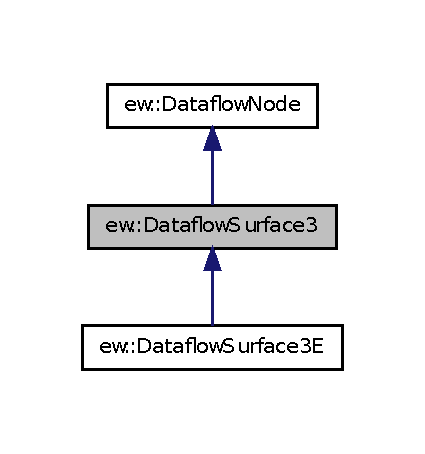
\includegraphics[width=204pt]{classew_1_1DataflowSurface3__inherit__graph}
\end{center}
\end{figure}
\subsubsection*{Public Member Functions}
\begin{DoxyCompactItemize}
\item 
int \hyperlink{classew_1_1DataflowSurface3_aab3c901dd150f4710c74c1cb1d140148}{get\_\-num\_\-points} () const 
\item 
int \hyperlink{classew_1_1DataflowSurface3_a2c3f79bba2d55ccfbe69d835af41d29e}{get\_\-num\_\-faces} () const 
\item 
const float $\ast$ \hyperlink{classew_1_1DataflowSurface3_aa585fbba3006c5a3a2c632cadd3f3cb7}{get\_\-points} () const 
\item 
const int $\ast$ \hyperlink{classew_1_1DataflowSurface3_abd809f7c907735fd027f6eb1f1f02be8}{get\_\-faces} () const 
\item 
const \hyperlink{classew_1_1Bbox3}{ew::Bbox3} $\ast$ \hyperlink{classew_1_1DataflowSurface3_aa68f8500425fc37c39bdf32e4b8c7ed1}{get\_\-bbox} () const 
\item 
void \hyperlink{classew_1_1DataflowSurface3_a42bc13a486803818b1db79cebac458d6}{make\_\-index} () const 
\item 
bool \hyperlink{classew_1_1DataflowSurface3_a81598b76d3bec4581fed07ac1858ca91}{index\_\-is\_\-made} () const 
\item 
double \hyperlink{classew_1_1DataflowSurface3_afd02a18df829a9608dac90940f603d83}{project} (int $\ast$face, double $\ast$coeffs, double $\ast$normal, double $\ast$proj, const double $\ast$inp) const 
\end{DoxyCompactItemize}


\subsubsection{Detailed Description}
\hyperlink{classew_1_1DataflowSurface3}{ew::DataflowSurface3} is the base class for nodes containing triangulated surfaces in $\mathbb{R}^3$.

\hyperlink{classew_1_1DataflowSurface3}{ew::DataflowSurface3} is a class without assignment or comparison. There are private member variables.

For efficient rendering of the same surface in multiple windows, an OpenGL display list is constructed containing the basic surface geometry commands. All windows displaying a given surface must share display lists. 

\subsubsection{Member Function Documentation}
\hypertarget{classew_1_1DataflowSurface3_aab3c901dd150f4710c74c1cb1d140148}{
\index{ew::DataflowSurface3@{ew::DataflowSurface3}!get\_\-num\_\-points@{get\_\-num\_\-points}}
\index{get\_\-num\_\-points@{get\_\-num\_\-points}!ew::DataflowSurface3@{ew::DataflowSurface3}}
\paragraph[{get\_\-num\_\-points}]{\setlength{\rightskip}{0pt plus 5cm}int ew::DataflowSurface3::get\_\-num\_\-points (
\begin{DoxyParamCaption}
{}
\end{DoxyParamCaption}
) const\hspace{0.3cm}{\ttfamily  \mbox{[}inline\mbox{]}}}\hfill}
\label{classew_1_1DataflowSurface3_aab3c901dd150f4710c74c1cb1d140148}
This will force the network into an updating phase. \begin{DoxyReturn}{Returns}
The number of points used in the surface. 
\end{DoxyReturn}
\hypertarget{classew_1_1DataflowSurface3_a2c3f79bba2d55ccfbe69d835af41d29e}{
\index{ew::DataflowSurface3@{ew::DataflowSurface3}!get\_\-num\_\-faces@{get\_\-num\_\-faces}}
\index{get\_\-num\_\-faces@{get\_\-num\_\-faces}!ew::DataflowSurface3@{ew::DataflowSurface3}}
\paragraph[{get\_\-num\_\-faces}]{\setlength{\rightskip}{0pt plus 5cm}int ew::DataflowSurface3::get\_\-num\_\-faces (
\begin{DoxyParamCaption}
{}
\end{DoxyParamCaption}
) const\hspace{0.3cm}{\ttfamily  \mbox{[}inline\mbox{]}}}\hfill}
\label{classew_1_1DataflowSurface3_a2c3f79bba2d55ccfbe69d835af41d29e}
This will force the network into an updating phase. \begin{DoxyReturn}{Returns}
The number of triangular faces in the surface. 
\end{DoxyReturn}
\hypertarget{classew_1_1DataflowSurface3_aa585fbba3006c5a3a2c632cadd3f3cb7}{
\index{ew::DataflowSurface3@{ew::DataflowSurface3}!get\_\-points@{get\_\-points}}
\index{get\_\-points@{get\_\-points}!ew::DataflowSurface3@{ew::DataflowSurface3}}
\paragraph[{get\_\-points}]{\setlength{\rightskip}{0pt plus 5cm}const float $\ast$ ew::DataflowSurface3::get\_\-points (
\begin{DoxyParamCaption}
{}
\end{DoxyParamCaption}
) const\hspace{0.3cm}{\ttfamily  \mbox{[}inline\mbox{]}}}\hfill}
\label{classew_1_1DataflowSurface3_aa585fbba3006c5a3a2c632cadd3f3cb7}
This will force the network into an updating phase. The pointer is valid until the node or a dependency of the node is changed. \begin{DoxyReturn}{Returns}
A pointer to the coordinates of the points used in the surface. 
\end{DoxyReturn}
\hypertarget{classew_1_1DataflowSurface3_abd809f7c907735fd027f6eb1f1f02be8}{
\index{ew::DataflowSurface3@{ew::DataflowSurface3}!get\_\-faces@{get\_\-faces}}
\index{get\_\-faces@{get\_\-faces}!ew::DataflowSurface3@{ew::DataflowSurface3}}
\paragraph[{get\_\-faces}]{\setlength{\rightskip}{0pt plus 5cm}const int $\ast$ ew::DataflowSurface3::get\_\-faces (
\begin{DoxyParamCaption}
{}
\end{DoxyParamCaption}
) const\hspace{0.3cm}{\ttfamily  \mbox{[}inline\mbox{]}}}\hfill}
\label{classew_1_1DataflowSurface3_abd809f7c907735fd027f6eb1f1f02be8}
This will force the network into an updating phase. The pointer is valid until the node or a dependency of the node is changed. \begin{DoxyReturn}{Returns}
A pointer to the indices of the points used in the surface. 
\end{DoxyReturn}
\hypertarget{classew_1_1DataflowSurface3_aa68f8500425fc37c39bdf32e4b8c7ed1}{
\index{ew::DataflowSurface3@{ew::DataflowSurface3}!get\_\-bbox@{get\_\-bbox}}
\index{get\_\-bbox@{get\_\-bbox}!ew::DataflowSurface3@{ew::DataflowSurface3}}
\paragraph[{get\_\-bbox}]{\setlength{\rightskip}{0pt plus 5cm}const {\bf ew::Bbox3} $\ast$ ew::DataflowSurface3::get\_\-bbox (
\begin{DoxyParamCaption}
{}
\end{DoxyParamCaption}
) const\hspace{0.3cm}{\ttfamily  \mbox{[}inline\mbox{]}}}\hfill}
\label{classew_1_1DataflowSurface3_aa68f8500425fc37c39bdf32e4b8c7ed1}
The pointer is valid until the node or a dependency of the node is changed. \begin{DoxyReturn}{Returns}
A pointer to the bounding box of the surface. 
\end{DoxyReturn}
\hypertarget{classew_1_1DataflowSurface3_a42bc13a486803818b1db79cebac458d6}{
\index{ew::DataflowSurface3@{ew::DataflowSurface3}!make\_\-index@{make\_\-index}}
\index{make\_\-index@{make\_\-index}!ew::DataflowSurface3@{ew::DataflowSurface3}}
\paragraph[{make\_\-index}]{\setlength{\rightskip}{0pt plus 5cm}void ew::DataflowSurface3::make\_\-index (
\begin{DoxyParamCaption}
{}
\end{DoxyParamCaption}
) const\hspace{0.3cm}{\ttfamily  \mbox{[}inline\mbox{]}}}\hfill}
\label{classew_1_1DataflowSurface3_a42bc13a486803818b1db79cebac458d6}
This makes the surface spatial index if it has not already been made since the surface was last changed. The spatial index is used by \hyperlink{classew_1_1DataflowSurface3_afd02a18df829a9608dac90940f603d83}{project}. \hypertarget{classew_1_1DataflowSurface3_a81598b76d3bec4581fed07ac1858ca91}{
\index{ew::DataflowSurface3@{ew::DataflowSurface3}!index\_\-is\_\-made@{index\_\-is\_\-made}}
\index{index\_\-is\_\-made@{index\_\-is\_\-made}!ew::DataflowSurface3@{ew::DataflowSurface3}}
\paragraph[{index\_\-is\_\-made}]{\setlength{\rightskip}{0pt plus 5cm}bool ew::DataflowSurface3::index\_\-is\_\-made (
\begin{DoxyParamCaption}
{}
\end{DoxyParamCaption}
) const\hspace{0.3cm}{\ttfamily  \mbox{[}inline\mbox{]}}}\hfill}
\label{classew_1_1DataflowSurface3_a81598b76d3bec4581fed07ac1858ca91}
\begin{DoxyReturn}{Returns}
{\ttfamily true} if the surface spatial index is up to date. 
\end{DoxyReturn}
\hypertarget{classew_1_1DataflowSurface3_afd02a18df829a9608dac90940f603d83}{
\index{ew::DataflowSurface3@{ew::DataflowSurface3}!project@{project}}
\index{project@{project}!ew::DataflowSurface3@{ew::DataflowSurface3}}
\paragraph[{project}]{\setlength{\rightskip}{0pt plus 5cm}double ew::DataflowSurface3::project (
\begin{DoxyParamCaption}
\item[{int $\ast$}]{ face, }
\item[{double $\ast$}]{ coeffs, }
\item[{double $\ast$}]{ normal, }
\item[{double $\ast$}]{ proj, }
\item[{const double $\ast$}]{ inp}
\end{DoxyParamCaption}
) const}\hfill}
\label{classew_1_1DataflowSurface3_afd02a18df829a9608dac90940f603d83}
This finds the nearest point on the surface to a given point. The surface spatial index will be made if it has not already been made. This might be time consuming. The timing of this delay can be controlled by calling \hyperlink{classew_1_1DataflowSurface3_a42bc13a486803818b1db79cebac458d6}{make\_\-index} beforehand. 
\begin{DoxyParams}{Parameters}
\item[\mbox{\tt[out]} {\em face}]The index of the face of the surface containing the nearest point. \item[\mbox{\tt[out]} {\em coeffs}]The coefficients of the nearest point when expressed as a linear combination of the vertices of the face. \item[\mbox{\tt[out]} {\em normal}]The interpolated normal at the nearest point. If a sensible normal cannot be calculated, an arbitrary unit vector is returned. \item[\mbox{\tt[out]} {\em proj}]The coordinates of the nearest point on the surface. \item[\mbox{\tt[in]} {\em inp}]The coordinates of the original point. \end{DoxyParams}
\begin{DoxyReturn}{Returns}
The distance from the original point to the projected point. 
\end{DoxyReturn}

\hypertarget{classew_1_1DataflowSurface3E}{
\subsection{ew::DataflowSurface3E Class Reference}
\label{classew_1_1DataflowSurface3E}\index{ew::DataflowSurface3E@{ew::DataflowSurface3E}}
}


Explicit Surface Node.  




{\ttfamily \#include $<$ew/DataflowSurface3E.h$>$}



Inheritance diagram for ew::DataflowSurface3E:
\nopagebreak
\begin{figure}[H]
\begin{center}
\leavevmode
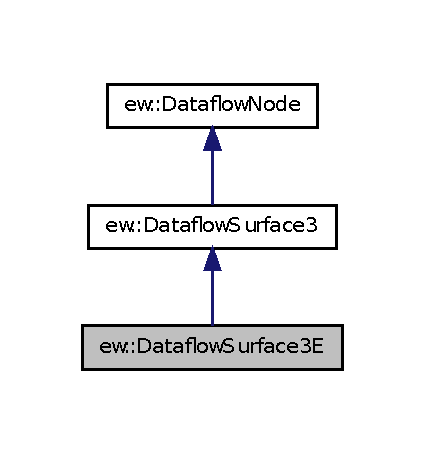
\includegraphics[width=204pt]{classew_1_1DataflowSurface3E__inherit__graph}
\end{center}
\end{figure}
\subsubsection*{Public Member Functions}
\begin{DoxyCompactItemize}
\item 
\hyperlink{classew_1_1DataflowSurface3E_ad4ab434027e31e3cf158c49f3eb15cd4}{DataflowSurface3E} (\hyperlink{classew_1_1DataflowNetwork}{ew::DataflowNetwork} $\ast$i\_\-network)
\item 
void \hyperlink{classew_1_1DataflowSurface3E_ae7cb9800ff79805c0249cb531a80f9f7}{set\_\-data} (\hyperlink{classew_1_1Surface3}{ew::Surface3} $\ast$data)
\item 
const \hyperlink{classew_1_1Surface3}{ew::Surface3} $\ast$ \hyperlink{classew_1_1DataflowSurface3E_a3d77b1d0cd97a05e4173eeb08a1f4994}{get\_\-data} () const 
\end{DoxyCompactItemize}


\subsubsection{Detailed Description}
\hyperlink{classew_1_1DataflowSurface3E}{ew::DataflowSurface3E} is a node containing an explicitly specified surface.

\hyperlink{classew_1_1DataflowSurface3E}{ew::DataflowSurface3E} objects may not be copied or compared. There are private member variables.

Nodes of this class do not depend on other nodes, but other nodes can depend on them. They are valid if they have some faces.

Initially and when reset, the node is empty. 

\subsubsection{Constructor \& Destructor Documentation}
\hypertarget{classew_1_1DataflowSurface3E_ad4ab434027e31e3cf158c49f3eb15cd4}{
\index{ew::DataflowSurface3E@{ew::DataflowSurface3E}!DataflowSurface3E@{DataflowSurface3E}}
\index{DataflowSurface3E@{DataflowSurface3E}!ew::DataflowSurface3E@{ew::DataflowSurface3E}}
\paragraph[{DataflowSurface3E}]{\setlength{\rightskip}{0pt plus 5cm}ew::DataflowSurface3E::DataflowSurface3E (
\begin{DoxyParamCaption}
\item[{{\bf ew::DataflowNetwork} $\ast$}]{ i\_\-network}
\end{DoxyParamCaption}
)\hspace{0.3cm}{\ttfamily  \mbox{[}explicit\mbox{]}}}\hfill}
\label{classew_1_1DataflowSurface3E_ad4ab434027e31e3cf158c49f3eb15cd4}
This creates an explicit surface node. 
\begin{DoxyParams}{Parameters}
\item[{\em i\_\-network}]The network this node should belong to. \end{DoxyParams}


\subsubsection{Member Function Documentation}
\hypertarget{classew_1_1DataflowSurface3E_ae7cb9800ff79805c0249cb531a80f9f7}{
\index{ew::DataflowSurface3E@{ew::DataflowSurface3E}!set\_\-data@{set\_\-data}}
\index{set\_\-data@{set\_\-data}!ew::DataflowSurface3E@{ew::DataflowSurface3E}}
\paragraph[{set\_\-data}]{\setlength{\rightskip}{0pt plus 5cm}void ew::DataflowSurface3E::set\_\-data (
\begin{DoxyParamCaption}
\item[{{\bf ew::Surface3} $\ast$}]{ data}
\end{DoxyParamCaption}
)}\hfill}
\label{classew_1_1DataflowSurface3E_ae7cb9800ff79805c0249cb531a80f9f7}
This transfers the surface data from the \hyperlink{classew_1_1Surface3}{ew::Surface3} object to the node. Afterwards, the \hyperlink{classew_1_1Surface3}{ew::Surface3} object is reset. \begin{DoxyPrecond}{Precondition}
This node must not be a cached node. 
\end{DoxyPrecond}

\begin{DoxyParams}{Parameters}
\item[{\em data}]The object containing the surface data. \end{DoxyParams}
\hypertarget{classew_1_1DataflowSurface3E_a3d77b1d0cd97a05e4173eeb08a1f4994}{
\index{ew::DataflowSurface3E@{ew::DataflowSurface3E}!get\_\-data@{get\_\-data}}
\index{get\_\-data@{get\_\-data}!ew::DataflowSurface3E@{ew::DataflowSurface3E}}
\paragraph[{get\_\-data}]{\setlength{\rightskip}{0pt plus 5cm}const {\bf ew::Surface3} $\ast$ ew::DataflowSurface3E::get\_\-data (
\begin{DoxyParamCaption}
{}
\end{DoxyParamCaption}
) const\hspace{0.3cm}{\ttfamily  \mbox{[}inline\mbox{]}}}\hfill}
\label{classew_1_1DataflowSurface3E_a3d77b1d0cd97a05e4173eeb08a1f4994}
\begin{DoxyReturn}{Returns}
A pointer to the internal surface data. 
\end{DoxyReturn}

\hypertarget{classew_1_1Dig3}{
\subsection{ew::Dig3 Class Reference}
\label{classew_1_1Dig3}\index{ew::Dig3@{ew::Dig3}}
}


Digitizing Application.  




{\ttfamily \#include $<$ew/Dig3.h$>$}

\subsubsection*{Public Types}
\begin{DoxyCompactItemize}
\item 
enum \hyperlink{classew_1_1Dig3_a218d7ccda5d476de1b2c8970f9c383ee}{space\_\-index\_\-t} \{ \hyperlink{classew_1_1Dig3_a218d7ccda5d476de1b2c8970f9c383eea8c1f651f962feb7eab6c19ee25118422}{SPACE\_\-TEMPLATE} =  0, 
\hyperlink{classew_1_1Dig3_a218d7ccda5d476de1b2c8970f9c383eea6efc6a44da15940b77ef70100ff927cc}{SPACE\_\-SPECIMEN} =  1
 \}
\item 
enum \hyperlink{classew_1_1Dig3_a52d5624e2591670cdb6e7fb212a55c9f}{tableau\_\-flags\_\-t} \{ \hyperlink{classew_1_1Dig3_a52d5624e2591670cdb6e7fb212a55c9fa49d067eb1fe80f6bcb69ff88b9611156}{TABLEAU\_\-VIEW} =  0x01, 
\hyperlink{classew_1_1Dig3_a52d5624e2591670cdb6e7fb212a55c9fac9c4c28672545c31088458b3767c03c7}{TABLEAU\_\-SETTINGS} =  0x02, 
\hyperlink{classew_1_1Dig3_a52d5624e2591670cdb6e7fb212a55c9fa1f77087df3ef36d5e24ec4ca71374d2d}{TABLEAU\_\-ALL} =  0x03
 \}
\end{DoxyCompactItemize}
\subsubsection*{Public Member Functions}
\begin{DoxyCompactItemize}
\item 
\hyperlink{classew_1_1Dig3_aabdbcd7bda62dda77dfa195023578051}{Dig3} (\hyperlink{classew_1_1DataflowNetwork}{ew::DataflowNetwork} $\ast$\hyperlink{classew_1_1Dig3_a94c1e034e60f4ca25cff64ee88ca86ab}{network})
\item 
\hyperlink{classew_1_1Dig3_a837f1989dfa80f5bf22eecafb055bf5c}{$\sim$Dig3} ()
\item 
int \hyperlink{classew_1_1Dig3_a44fe876fbf8342d6edd2355729afc495}{get\_\-n\_\-views} () const 
\item 
\hyperlink{classew_1_1Dig3View}{ew::Dig3View} $\ast$const $\ast$ \hyperlink{classew_1_1Dig3_a5ddec0535d0680a0b37616dbc4eee042}{get\_\-views} () const 
\item 
\hyperlink{classew_1_1Dig3Space}{ew::Dig3Space} $\ast$const $\ast$ \hyperlink{classew_1_1Dig3_ad8f02ea649e872543988eaf56ac8858f}{get\_\-spaces} () const 
\item 
const \hyperlink{classew_1_1DataflowSpline3}{ew::DataflowSpline3} $\ast$ \hyperlink{classew_1_1Dig3_ab163ea18f43b5c753b1b18b1523b4886}{get\_\-spline\_\-node} () const 
\item 
void \hyperlink{classew_1_1Dig3_a805ae977646c8b6c3bd1bff65c700569}{save\_\-tableau} (\hyperlink{classew_1_1Dig3Tableau}{ew::Dig3Tableau} $\ast$outp, int template\_\-main, int template\_\-slice, int specimen\_\-main, int specimen\_\-slice)
\item 
void \hyperlink{classew_1_1Dig3_aa20f2ab4ae20bfa1600ff4a32fbb2182}{load\_\-tableau} (const \hyperlink{classew_1_1Dig3Tableau}{ew::Dig3Tableau} $\ast$inp, int view, unsigned int flags)
\item 
void \hyperlink{classew_1_1Dig3_a9683b9f765ca282b010431c4e8b1888d}{interpolate\_\-tableau} (const \hyperlink{classew_1_1Dig3Tableau}{ew::Dig3Tableau} $\ast$inp1, const \hyperlink{classew_1_1Dig3Tableau}{ew::Dig3Tableau} $\ast$inp2, double e, int view)
\end{DoxyCompactItemize}
\subsubsection*{Public Attributes}
\begin{DoxyCompactItemize}
\item 
\hyperlink{classew_1_1DataflowNetwork}{ew::DataflowNetwork} $\ast$const \hyperlink{classew_1_1Dig3_a94c1e034e60f4ca25cff64ee88ca86ab}{network}
\end{DoxyCompactItemize}


\subsubsection{Detailed Description}
\hyperlink{classew_1_1Dig3}{ew::Dig3} implements a 3D digitizing application.

\hyperlink{classew_1_1Dig3}{ew::Dig3} is a class without assignment or comparison. There are private member variables.

An \hyperlink{classew_1_1Dig3}{ew::Dig3} maintains 2 space elements, the template and the specimen.

View elements can be added and removed by creating or destroying \hyperlink{classew_1_1Dig3View}{ew::Dig3View} objects. 

\subsubsection{Member Enumeration Documentation}
\hypertarget{classew_1_1Dig3_a218d7ccda5d476de1b2c8970f9c383ee}{
\index{ew::Dig3@{ew::Dig3}!space\_\-index\_\-t@{space\_\-index\_\-t}}
\index{space\_\-index\_\-t@{space\_\-index\_\-t}!ew::Dig3@{ew::Dig3}}
\paragraph[{space\_\-index\_\-t}]{\setlength{\rightskip}{0pt plus 5cm}enum {\bf ew::Dig3::space\_\-index\_\-t}}\hfill}
\label{classew_1_1Dig3_a218d7ccda5d476de1b2c8970f9c383ee}
These are the indices of the 2 spaces in the array of spaces. \begin{Desc}
\item[Enumerator: ]\par
\begin{description}
\index{SPACE\_\-TEMPLATE@{SPACE\_\-TEMPLATE}!ew::Dig3@{ew::Dig3}}\index{ew::Dig3@{ew::Dig3}!SPACE\_\-TEMPLATE@{SPACE\_\-TEMPLATE}}\item[{\em 
\hypertarget{classew_1_1Dig3_a218d7ccda5d476de1b2c8970f9c383eea8c1f651f962feb7eab6c19ee25118422}{
SPACE\_\-TEMPLATE}
\label{classew_1_1Dig3_a218d7ccda5d476de1b2c8970f9c383eea8c1f651f962feb7eab6c19ee25118422}
}]The index of the template space. \index{SPACE\_\-SPECIMEN@{SPACE\_\-SPECIMEN}!ew::Dig3@{ew::Dig3}}\index{ew::Dig3@{ew::Dig3}!SPACE\_\-SPECIMEN@{SPACE\_\-SPECIMEN}}\item[{\em 
\hypertarget{classew_1_1Dig3_a218d7ccda5d476de1b2c8970f9c383eea6efc6a44da15940b77ef70100ff927cc}{
SPACE\_\-SPECIMEN}
\label{classew_1_1Dig3_a218d7ccda5d476de1b2c8970f9c383eea6efc6a44da15940b77ef70100ff927cc}
}]The index of the specimen space. \end{description}
\end{Desc}

\hypertarget{classew_1_1Dig3_a52d5624e2591670cdb6e7fb212a55c9f}{
\index{ew::Dig3@{ew::Dig3}!tableau\_\-flags\_\-t@{tableau\_\-flags\_\-t}}
\index{tableau\_\-flags\_\-t@{tableau\_\-flags\_\-t}!ew::Dig3@{ew::Dig3}}
\paragraph[{tableau\_\-flags\_\-t}]{\setlength{\rightskip}{0pt plus 5cm}enum {\bf ew::Dig3::tableau\_\-flags\_\-t}}\hfill}
\label{classew_1_1Dig3_a52d5624e2591670cdb6e7fb212a55c9f}
These are flags that can be or-\/ed and passed to \hyperlink{classew_1_1Dig3_aa20f2ab4ae20bfa1600ff4a32fbb2182}{load\_\-tableau}. \begin{Desc}
\item[Enumerator: ]\par
\begin{description}
\index{TABLEAU\_\-VIEW@{TABLEAU\_\-VIEW}!ew::Dig3@{ew::Dig3}}\index{ew::Dig3@{ew::Dig3}!TABLEAU\_\-VIEW@{TABLEAU\_\-VIEW}}\item[{\em 
\hypertarget{classew_1_1Dig3_a52d5624e2591670cdb6e7fb212a55c9fa49d067eb1fe80f6bcb69ff88b9611156}{
TABLEAU\_\-VIEW}
\label{classew_1_1Dig3_a52d5624e2591670cdb6e7fb212a55c9fa49d067eb1fe80f6bcb69ff88b9611156}
}]Set the view mapping. \index{TABLEAU\_\-SETTINGS@{TABLEAU\_\-SETTINGS}!ew::Dig3@{ew::Dig3}}\index{ew::Dig3@{ew::Dig3}!TABLEAU\_\-SETTINGS@{TABLEAU\_\-SETTINGS}}\item[{\em 
\hypertarget{classew_1_1Dig3_a52d5624e2591670cdb6e7fb212a55c9fac9c4c28672545c31088458b3767c03c7}{
TABLEAU\_\-SETTINGS}
\label{classew_1_1Dig3_a52d5624e2591670cdb6e7fb212a55c9fac9c4c28672545c31088458b3767c03c7}
}]Set the settings. \index{TABLEAU\_\-ALL@{TABLEAU\_\-ALL}!ew::Dig3@{ew::Dig3}}\index{ew::Dig3@{ew::Dig3}!TABLEAU\_\-ALL@{TABLEAU\_\-ALL}}\item[{\em 
\hypertarget{classew_1_1Dig3_a52d5624e2591670cdb6e7fb212a55c9fa1f77087df3ef36d5e24ec4ca71374d2d}{
TABLEAU\_\-ALL}
\label{classew_1_1Dig3_a52d5624e2591670cdb6e7fb212a55c9fa1f77087df3ef36d5e24ec4ca71374d2d}
}]Set everything. \end{description}
\end{Desc}



\subsubsection{Constructor \& Destructor Documentation}
\hypertarget{classew_1_1Dig3_aabdbcd7bda62dda77dfa195023578051}{
\index{ew::Dig3@{ew::Dig3}!Dig3@{Dig3}}
\index{Dig3@{Dig3}!ew::Dig3@{ew::Dig3}}
\paragraph[{Dig3}]{\setlength{\rightskip}{0pt plus 5cm}ew::Dig3::Dig3 (
\begin{DoxyParamCaption}
\item[{{\bf ew::DataflowNetwork} $\ast$}]{ network}
\end{DoxyParamCaption}
)\hspace{0.3cm}{\ttfamily  \mbox{[}explicit\mbox{]}}}\hfill}
\label{classew_1_1Dig3_aabdbcd7bda62dda77dfa195023578051}
This creates an empty digitizing application. 
\begin{DoxyParams}{Parameters}
\item[{\em network}]A pointer to a dataflow network. \end{DoxyParams}
\hypertarget{classew_1_1Dig3_a837f1989dfa80f5bf22eecafb055bf5c}{
\index{ew::Dig3@{ew::Dig3}!$\sim$Dig3@{$\sim$Dig3}}
\index{$\sim$Dig3@{$\sim$Dig3}!ew::Dig3@{ew::Dig3}}
\paragraph[{$\sim$Dig3}]{\setlength{\rightskip}{0pt plus 5cm}ew::Dig3::$\sim$Dig3 (
\begin{DoxyParamCaption}
{}
\end{DoxyParamCaption}
)}\hfill}
\label{classew_1_1Dig3_a837f1989dfa80f5bf22eecafb055bf5c}
This destroys the digitizing application. Any \hyperlink{classew_1_1Dig3View}{ew::Dig3View} widgets associated with it are also destroyed. 

\subsubsection{Member Function Documentation}
\hypertarget{classew_1_1Dig3_a44fe876fbf8342d6edd2355729afc495}{
\index{ew::Dig3@{ew::Dig3}!get\_\-n\_\-views@{get\_\-n\_\-views}}
\index{get\_\-n\_\-views@{get\_\-n\_\-views}!ew::Dig3@{ew::Dig3}}
\paragraph[{get\_\-n\_\-views}]{\setlength{\rightskip}{0pt plus 5cm}int ew::Dig3::get\_\-n\_\-views (
\begin{DoxyParamCaption}
{}
\end{DoxyParamCaption}
) const\hspace{0.3cm}{\ttfamily  \mbox{[}inline\mbox{]}}}\hfill}
\label{classew_1_1Dig3_a44fe876fbf8342d6edd2355729afc495}
\begin{DoxyReturn}{Returns}
The number of views. 
\end{DoxyReturn}
\hypertarget{classew_1_1Dig3_a5ddec0535d0680a0b37616dbc4eee042}{
\index{ew::Dig3@{ew::Dig3}!get\_\-views@{get\_\-views}}
\index{get\_\-views@{get\_\-views}!ew::Dig3@{ew::Dig3}}
\paragraph[{get\_\-views}]{\setlength{\rightskip}{0pt plus 5cm}{\bf ew::Dig3View} $\ast$const $\ast$ ew::Dig3::get\_\-views (
\begin{DoxyParamCaption}
{}
\end{DoxyParamCaption}
) const\hspace{0.3cm}{\ttfamily  \mbox{[}inline\mbox{]}}}\hfill}
\label{classew_1_1Dig3_a5ddec0535d0680a0b37616dbc4eee042}
\begin{DoxyReturn}{Returns}
The view index. 
\end{DoxyReturn}
\hypertarget{classew_1_1Dig3_ad8f02ea649e872543988eaf56ac8858f}{
\index{ew::Dig3@{ew::Dig3}!get\_\-spaces@{get\_\-spaces}}
\index{get\_\-spaces@{get\_\-spaces}!ew::Dig3@{ew::Dig3}}
\paragraph[{get\_\-spaces}]{\setlength{\rightskip}{0pt plus 5cm}{\bf ew::Dig3Space} $\ast$const $\ast$ ew::Dig3::get\_\-spaces (
\begin{DoxyParamCaption}
{}
\end{DoxyParamCaption}
) const\hspace{0.3cm}{\ttfamily  \mbox{[}inline\mbox{]}}}\hfill}
\label{classew_1_1Dig3_ad8f02ea649e872543988eaf56ac8858f}
\begin{DoxyReturn}{Returns}
The space index. There are always 2 spaces and the index is constant. 
\end{DoxyReturn}
\hypertarget{classew_1_1Dig3_ab163ea18f43b5c753b1b18b1523b4886}{
\index{ew::Dig3@{ew::Dig3}!get\_\-spline\_\-node@{get\_\-spline\_\-node}}
\index{get\_\-spline\_\-node@{get\_\-spline\_\-node}!ew::Dig3@{ew::Dig3}}
\paragraph[{get\_\-spline\_\-node}]{\setlength{\rightskip}{0pt plus 5cm}const {\bf ew::DataflowSpline3} $\ast$ ew::Dig3::get\_\-spline\_\-node (
\begin{DoxyParamCaption}
{}
\end{DoxyParamCaption}
) const\hspace{0.3cm}{\ttfamily  \mbox{[}inline\mbox{]}}}\hfill}
\label{classew_1_1Dig3_ab163ea18f43b5c753b1b18b1523b4886}
\begin{DoxyReturn}{Returns}
A pointer to the spline node that this \hyperlink{classew_1_1Dig3}{ew::Dig3} manages. 
\end{DoxyReturn}
\hypertarget{classew_1_1Dig3_a805ae977646c8b6c3bd1bff65c700569}{
\index{ew::Dig3@{ew::Dig3}!save\_\-tableau@{save\_\-tableau}}
\index{save\_\-tableau@{save\_\-tableau}!ew::Dig3@{ew::Dig3}}
\paragraph[{save\_\-tableau}]{\setlength{\rightskip}{0pt plus 5cm}void ew::Dig3::save\_\-tableau (
\begin{DoxyParamCaption}
\item[{{\bf ew::Dig3Tableau} $\ast$}]{ outp, }
\item[{int}]{ template\_\-main, }
\item[{int}]{ template\_\-slice, }
\item[{int}]{ specimen\_\-main, }
\item[{int}]{ specimen\_\-slice}
\end{DoxyParamCaption}
)}\hfill}
\label{classew_1_1Dig3_a805ae977646c8b6c3bd1bff65c700569}
This creates a tableau record from the indicated views, specified by index. The form filename fields of the tableau are left blank, and must be explicitly set. 
\begin{DoxyParams}{Parameters}
\item[{\em outp}]Where to store the tableau record. \item[{\em template\_\-main}]The index of a template main view to record. \item[{\em template\_\-slice}]The index of a template slice view to record. \item[{\em specimen\_\-main}]The index of a specimen main view to record. \item[{\em specimen\_\-slice}]The index of a specimen slice view to record. \end{DoxyParams}
\hypertarget{classew_1_1Dig3_aa20f2ab4ae20bfa1600ff4a32fbb2182}{
\index{ew::Dig3@{ew::Dig3}!load\_\-tableau@{load\_\-tableau}}
\index{load\_\-tableau@{load\_\-tableau}!ew::Dig3@{ew::Dig3}}
\paragraph[{load\_\-tableau}]{\setlength{\rightskip}{0pt plus 5cm}void ew::Dig3::load\_\-tableau (
\begin{DoxyParamCaption}
\item[{const {\bf ew::Dig3Tableau} $\ast$}]{ inp, }
\item[{int}]{ view, }
\item[{unsigned int}]{ flags}
\end{DoxyParamCaption}
)}\hfill}
\label{classew_1_1Dig3_aa20f2ab4ae20bfa1600ff4a32fbb2182}
This applies a tableau record to the indicated view. The type of view and its space determine which part of the record is applied. The form filename fields are not applied. The forms must be explicitly set beforehand. 
\begin{DoxyParams}{Parameters}
\item[{\em inp}]The tableau to apply. \item[{\em view}]The index of the view to apply it to. \item[{\em flags}]Flags of type \hyperlink{classew_1_1Dig3_a52d5624e2591670cdb6e7fb212a55c9f}{tableau\_\-flags\_\-t} indicating which parts of the tableau record to apply. \end{DoxyParams}
\hypertarget{classew_1_1Dig3_a9683b9f765ca282b010431c4e8b1888d}{
\index{ew::Dig3@{ew::Dig3}!interpolate\_\-tableau@{interpolate\_\-tableau}}
\index{interpolate\_\-tableau@{interpolate\_\-tableau}!ew::Dig3@{ew::Dig3}}
\paragraph[{interpolate\_\-tableau}]{\setlength{\rightskip}{0pt plus 5cm}void ew::Dig3::interpolate\_\-tableau (
\begin{DoxyParamCaption}
\item[{const {\bf ew::Dig3Tableau} $\ast$}]{ inp1, }
\item[{const {\bf ew::Dig3Tableau} $\ast$}]{ inp2, }
\item[{double}]{ e, }
\item[{int}]{ view}
\end{DoxyParamCaption}
)}\hfill}
\label{classew_1_1Dig3_a9683b9f765ca282b010431c4e8b1888d}
This interpolates between tableau records and applies the result to the indicated view. Only the views are applied. The settings of the tableau and the forms cannot be interpolated and need to be manually applied when a new frame is reached in a filmstrip. 
\begin{DoxyParams}{Parameters}
\item[{\em inp1,inp2}]The tableaus to interpolate. \item[{\em e}]The interpolation parameter, with 0.0 corresponding to {\itshape inp1\/} and 1.0 to {\itshape inp\/}. {\itshape e\/} is not restricted to \mbox{[}0.0, 1.0\mbox{]}. \item[{\em view}]The index of the view to apply it to. \end{DoxyParams}


\subsubsection{Member Data Documentation}
\hypertarget{classew_1_1Dig3_a94c1e034e60f4ca25cff64ee88ca86ab}{
\index{ew::Dig3@{ew::Dig3}!network@{network}}
\index{network@{network}!ew::Dig3@{ew::Dig3}}
\paragraph[{network}]{\setlength{\rightskip}{0pt plus 5cm}{\bf ew::DataflowNetwork} $\ast$const {\bf ew::Dig3::network}}\hfill}
\label{classew_1_1Dig3_a94c1e034e60f4ca25cff64ee88ca86ab}
This points to the \hyperlink{classew_1_1DataflowNetwork}{ew::DataflowNetwork} that this \hyperlink{classew_1_1Dig3}{ew::Dig3} was created with. 
\hypertarget{classew_1_1Dig3SetCurve}{
\subsection{ew::Dig3SetCurve Class Reference}
\label{classew_1_1Dig3SetCurve}\index{ew::Dig3SetCurve@{ew::Dig3SetCurve}}
}


Curve Element.  




{\ttfamily \#include $<$ew/Dig3SetCurve.h$>$}

\subsubsection*{Public Member Functions}
\begin{DoxyCompactItemize}
\item 
\hyperlink{classew_1_1Dig3SetCurve_ac1f9c404a6534de970e2f3420a65adc2}{Dig3SetCurve} ()
\item 
bool \hyperlink{classew_1_1Dig3SetCurve_acaf106b1be917bae9aca68fd463c6596}{operator==} (const \hyperlink{classew_1_1Dig3SetCurve}{ew::Dig3SetCurve} \&a) const 
\item 
bool \hyperlink{classew_1_1Dig3SetCurve_a30f98f13b265d50a12ce79e046255f86}{operator!=} (const \hyperlink{classew_1_1Dig3SetCurve}{ew::Dig3SetCurve} \&a) const 
\end{DoxyCompactItemize}
\subsubsection*{Public Attributes}
\begin{DoxyCompactItemize}
\item 
std::string \hyperlink{classew_1_1Dig3SetCurve_a2e33ff75ce3983664e36a8ef6743cb87}{id}
\item 
bool \hyperlink{classew_1_1Dig3SetCurve_a863b47d06046cf374792227495b92fb0}{show\_\-in\_\-main}
\item 
bool \hyperlink{classew_1_1Dig3SetCurve_af653d84915b2581c139d6928c2943d00}{show\_\-in\_\-slice}
\item 
unsigned char \hyperlink{classew_1_1Dig3SetCurve_a92f3ffc02cb571c898a0f5af2ba6a096}{col} \mbox{[}3\mbox{]}
\end{DoxyCompactItemize}


\subsubsection{Detailed Description}
\hyperlink{classew_1_1Dig3SetCurve}{ew::Dig3SetCurve} contains data for a curve element of ew::Tableau.

\hyperlink{classew_1_1Dig3SetCurve}{ew::Dig3SetCurve} is a data structure that supports default construction, copy construction, assignment and equality comparison. 

\subsubsection{Constructor \& Destructor Documentation}
\hypertarget{classew_1_1Dig3SetCurve_ac1f9c404a6534de970e2f3420a65adc2}{
\index{ew::Dig3SetCurve@{ew::Dig3SetCurve}!Dig3SetCurve@{Dig3SetCurve}}
\index{Dig3SetCurve@{Dig3SetCurve}!ew::Dig3SetCurve@{ew::Dig3SetCurve}}
\paragraph[{Dig3SetCurve}]{\setlength{\rightskip}{0pt plus 5cm}ew::Dig3SetCurve::Dig3SetCurve (
\begin{DoxyParamCaption}
{}
\end{DoxyParamCaption}
)\hspace{0.3cm}{\ttfamily  \mbox{[}inline\mbox{]}}}\hfill}
\label{classew_1_1Dig3SetCurve_ac1f9c404a6534de970e2f3420a65adc2}
This sets intrinsic member variables to their default values. 

\subsubsection{Member Function Documentation}
\hypertarget{classew_1_1Dig3SetCurve_acaf106b1be917bae9aca68fd463c6596}{
\index{ew::Dig3SetCurve@{ew::Dig3SetCurve}!operator==@{operator==}}
\index{operator==@{operator==}!ew::Dig3SetCurve@{ew::Dig3SetCurve}}
\paragraph[{operator==}]{\setlength{\rightskip}{0pt plus 5cm}bool ew::Dig3SetCurve::operator== (
\begin{DoxyParamCaption}
\item[{const {\bf ew::Dig3SetCurve} \&}]{ a}
\end{DoxyParamCaption}
) const\hspace{0.3cm}{\ttfamily  \mbox{[}inline\mbox{]}}}\hfill}
\label{classew_1_1Dig3SetCurve_acaf106b1be917bae9aca68fd463c6596}
Compares this element with another, member by member. 
\begin{DoxyParams}{Parameters}
\item[{\em a}]the other element \end{DoxyParams}
\hypertarget{classew_1_1Dig3SetCurve_a30f98f13b265d50a12ce79e046255f86}{
\index{ew::Dig3SetCurve@{ew::Dig3SetCurve}!operator!=@{operator!=}}
\index{operator!=@{operator!=}!ew::Dig3SetCurve@{ew::Dig3SetCurve}}
\paragraph[{operator!=}]{\setlength{\rightskip}{0pt plus 5cm}bool ew::Dig3SetCurve::operator!= (
\begin{DoxyParamCaption}
\item[{const {\bf ew::Dig3SetCurve} \&}]{ a}
\end{DoxyParamCaption}
) const\hspace{0.3cm}{\ttfamily  \mbox{[}inline\mbox{]}}}\hfill}
\label{classew_1_1Dig3SetCurve_a30f98f13b265d50a12ce79e046255f86}
Compares this element with another, member by member. 
\begin{DoxyParams}{Parameters}
\item[{\em a}]the other element \end{DoxyParams}


\subsubsection{Member Data Documentation}
\hypertarget{classew_1_1Dig3SetCurve_a2e33ff75ce3983664e36a8ef6743cb87}{
\index{ew::Dig3SetCurve@{ew::Dig3SetCurve}!id@{id}}
\index{id@{id}!ew::Dig3SetCurve@{ew::Dig3SetCurve}}
\paragraph[{id}]{\setlength{\rightskip}{0pt plus 5cm}std::string {\bf ew::Dig3SetCurve::id}}\hfill}
\label{classew_1_1Dig3SetCurve_a2e33ff75ce3983664e36a8ef6743cb87}
The \hyperlink{classew_1_1Form3Curve_a2bb3648bb9d075b67572de31ceb4f9c9}{ew::Form3Curve::id} of the curve this field should apply to. \hypertarget{classew_1_1Dig3SetCurve_a863b47d06046cf374792227495b92fb0}{
\index{ew::Dig3SetCurve@{ew::Dig3SetCurve}!show\_\-in\_\-main@{show\_\-in\_\-main}}
\index{show\_\-in\_\-main@{show\_\-in\_\-main}!ew::Dig3SetCurve@{ew::Dig3SetCurve}}
\paragraph[{show\_\-in\_\-main}]{\setlength{\rightskip}{0pt plus 5cm}bool {\bf ew::Dig3SetCurve::show\_\-in\_\-main}}\hfill}
\label{classew_1_1Dig3SetCurve_a863b47d06046cf374792227495b92fb0}
{\ttfamily true} if the curve should be displayed in the main view. The default is {\ttfamily true}. \hypertarget{classew_1_1Dig3SetCurve_af653d84915b2581c139d6928c2943d00}{
\index{ew::Dig3SetCurve@{ew::Dig3SetCurve}!show\_\-in\_\-slice@{show\_\-in\_\-slice}}
\index{show\_\-in\_\-slice@{show\_\-in\_\-slice}!ew::Dig3SetCurve@{ew::Dig3SetCurve}}
\paragraph[{show\_\-in\_\-slice}]{\setlength{\rightskip}{0pt plus 5cm}bool {\bf ew::Dig3SetCurve::show\_\-in\_\-slice}}\hfill}
\label{classew_1_1Dig3SetCurve_af653d84915b2581c139d6928c2943d00}
{\ttfamily true} if the curve should be displayed in the slice view. The default is {\ttfamily true}. \hypertarget{classew_1_1Dig3SetCurve_a92f3ffc02cb571c898a0f5af2ba6a096}{
\index{ew::Dig3SetCurve@{ew::Dig3SetCurve}!col@{col}}
\index{col@{col}!ew::Dig3SetCurve@{ew::Dig3SetCurve}}
\paragraph[{col}]{\setlength{\rightskip}{0pt plus 5cm}unsigned char {\bf ew::Dig3SetCurve::col}\mbox{[}3\mbox{]}}\hfill}
\label{classew_1_1Dig3SetCurve_a92f3ffc02cb571c898a0f5af2ba6a096}
The colour of the curve. The default is \mbox{[}128, 128, 128\mbox{]}. 
\hypertarget{classew_1_1Dig3SetSurface}{
\subsection{ew::Dig3SetSurface Class Reference}
\label{classew_1_1Dig3SetSurface}\index{ew::Dig3SetSurface@{ew::Dig3SetSurface}}
}


Surface Element.  




{\ttfamily \#include $<$ew/Dig3SetSurface.h$>$}

\subsubsection*{Public Member Functions}
\begin{DoxyCompactItemize}
\item 
\hyperlink{classew_1_1Dig3SetSurface_a426b3d9fa1363915d4c0972bb80d5636}{Dig3SetSurface} ()
\item 
bool \hyperlink{classew_1_1Dig3SetSurface_af4111aad020b0af73f43356dff480d24}{operator==} (const \hyperlink{classew_1_1Dig3SetSurface}{ew::Dig3SetSurface} \&a) const 
\item 
bool \hyperlink{classew_1_1Dig3SetSurface_aba2c063ee81653fc9e7872f5bfba747e}{operator!=} (const \hyperlink{classew_1_1Dig3SetSurface}{ew::Dig3SetSurface} \&a) const 
\end{DoxyCompactItemize}
\subsubsection*{Public Attributes}
\begin{DoxyCompactItemize}
\item 
std::string \hyperlink{classew_1_1Dig3SetSurface_aef9a8a1de88c69d590443a7fabb16f7c}{id}
\item 
bool \hyperlink{classew_1_1Dig3SetSurface_ad71bb9c721004e888f70c89d90fd6016}{show\_\-in\_\-main}
\item 
bool \hyperlink{classew_1_1Dig3SetSurface_a11a98c149d5f62f0d5c3b2230be82dfa}{show\_\-in\_\-slice}
\item 
unsigned char \hyperlink{classew_1_1Dig3SetSurface_aa067f664f7409bdab4f31a2facfc981d}{front\_\-col} \mbox{[}3\mbox{]}
\item 
unsigned char \hyperlink{classew_1_1Dig3SetSurface_ab5bb87bc9fb4bbf52dde7106f3cc4be1}{back\_\-col} \mbox{[}3\mbox{]}
\end{DoxyCompactItemize}


\subsubsection{Detailed Description}
\hyperlink{classew_1_1Dig3SetSurface}{ew::Dig3SetSurface} contains data for a surface element of ew::Tableau.

\hyperlink{classew_1_1Dig3SetSurface}{ew::Dig3SetSurface} is a data structure that supports default construction, copy construction, assignment and equality comparison. 

\subsubsection{Constructor \& Destructor Documentation}
\hypertarget{classew_1_1Dig3SetSurface_a426b3d9fa1363915d4c0972bb80d5636}{
\index{ew::Dig3SetSurface@{ew::Dig3SetSurface}!Dig3SetSurface@{Dig3SetSurface}}
\index{Dig3SetSurface@{Dig3SetSurface}!ew::Dig3SetSurface@{ew::Dig3SetSurface}}
\paragraph[{Dig3SetSurface}]{\setlength{\rightskip}{0pt plus 5cm}ew::Dig3SetSurface::Dig3SetSurface (
\begin{DoxyParamCaption}
{}
\end{DoxyParamCaption}
)\hspace{0.3cm}{\ttfamily  \mbox{[}inline\mbox{]}}}\hfill}
\label{classew_1_1Dig3SetSurface_a426b3d9fa1363915d4c0972bb80d5636}
This sets intrinsic member variables to their default values. 

\subsubsection{Member Function Documentation}
\hypertarget{classew_1_1Dig3SetSurface_af4111aad020b0af73f43356dff480d24}{
\index{ew::Dig3SetSurface@{ew::Dig3SetSurface}!operator==@{operator==}}
\index{operator==@{operator==}!ew::Dig3SetSurface@{ew::Dig3SetSurface}}
\paragraph[{operator==}]{\setlength{\rightskip}{0pt plus 5cm}bool ew::Dig3SetSurface::operator== (
\begin{DoxyParamCaption}
\item[{const {\bf ew::Dig3SetSurface} \&}]{ a}
\end{DoxyParamCaption}
) const\hspace{0.3cm}{\ttfamily  \mbox{[}inline\mbox{]}}}\hfill}
\label{classew_1_1Dig3SetSurface_af4111aad020b0af73f43356dff480d24}
Compares this element with another, member by member. 
\begin{DoxyParams}{Parameters}
\item[{\em a}]the other element \end{DoxyParams}
\hypertarget{classew_1_1Dig3SetSurface_aba2c063ee81653fc9e7872f5bfba747e}{
\index{ew::Dig3SetSurface@{ew::Dig3SetSurface}!operator!=@{operator!=}}
\index{operator!=@{operator!=}!ew::Dig3SetSurface@{ew::Dig3SetSurface}}
\paragraph[{operator!=}]{\setlength{\rightskip}{0pt plus 5cm}bool ew::Dig3SetSurface::operator!= (
\begin{DoxyParamCaption}
\item[{const {\bf ew::Dig3SetSurface} \&}]{ a}
\end{DoxyParamCaption}
) const\hspace{0.3cm}{\ttfamily  \mbox{[}inline\mbox{]}}}\hfill}
\label{classew_1_1Dig3SetSurface_aba2c063ee81653fc9e7872f5bfba747e}
Compares this element with another, member by member. 
\begin{DoxyParams}{Parameters}
\item[{\em a}]the other element \end{DoxyParams}


\subsubsection{Member Data Documentation}
\hypertarget{classew_1_1Dig3SetSurface_aef9a8a1de88c69d590443a7fabb16f7c}{
\index{ew::Dig3SetSurface@{ew::Dig3SetSurface}!id@{id}}
\index{id@{id}!ew::Dig3SetSurface@{ew::Dig3SetSurface}}
\paragraph[{id}]{\setlength{\rightskip}{0pt plus 5cm}std::string {\bf ew::Dig3SetSurface::id}}\hfill}
\label{classew_1_1Dig3SetSurface_aef9a8a1de88c69d590443a7fabb16f7c}
The \hyperlink{classew_1_1Form3Surface_aa207964ce409cd2cd7b0d4a02ad18d5a}{ew::Form3Surface::id} of the surface this field should apply to. \hypertarget{classew_1_1Dig3SetSurface_ad71bb9c721004e888f70c89d90fd6016}{
\index{ew::Dig3SetSurface@{ew::Dig3SetSurface}!show\_\-in\_\-main@{show\_\-in\_\-main}}
\index{show\_\-in\_\-main@{show\_\-in\_\-main}!ew::Dig3SetSurface@{ew::Dig3SetSurface}}
\paragraph[{show\_\-in\_\-main}]{\setlength{\rightskip}{0pt plus 5cm}bool {\bf ew::Dig3SetSurface::show\_\-in\_\-main}}\hfill}
\label{classew_1_1Dig3SetSurface_ad71bb9c721004e888f70c89d90fd6016}
{\ttfamily true} if the surface should be displayed in the main view. The default is {\ttfamily true}. \hypertarget{classew_1_1Dig3SetSurface_a11a98c149d5f62f0d5c3b2230be82dfa}{
\index{ew::Dig3SetSurface@{ew::Dig3SetSurface}!show\_\-in\_\-slice@{show\_\-in\_\-slice}}
\index{show\_\-in\_\-slice@{show\_\-in\_\-slice}!ew::Dig3SetSurface@{ew::Dig3SetSurface}}
\paragraph[{show\_\-in\_\-slice}]{\setlength{\rightskip}{0pt plus 5cm}bool {\bf ew::Dig3SetSurface::show\_\-in\_\-slice}}\hfill}
\label{classew_1_1Dig3SetSurface_a11a98c149d5f62f0d5c3b2230be82dfa}
{\ttfamily true} if the surface should be displayed in the slice view. The default is {\ttfamily true}. \hypertarget{classew_1_1Dig3SetSurface_aa067f664f7409bdab4f31a2facfc981d}{
\index{ew::Dig3SetSurface@{ew::Dig3SetSurface}!front\_\-col@{front\_\-col}}
\index{front\_\-col@{front\_\-col}!ew::Dig3SetSurface@{ew::Dig3SetSurface}}
\paragraph[{front\_\-col}]{\setlength{\rightskip}{0pt plus 5cm}unsigned char {\bf ew::Dig3SetSurface::front\_\-col}\mbox{[}3\mbox{]}}\hfill}
\label{classew_1_1Dig3SetSurface_aa067f664f7409bdab4f31a2facfc981d}
The colour of the front side of the surface. The default is \mbox{[}128, 128, 128\mbox{]}. \hypertarget{classew_1_1Dig3SetSurface_ab5bb87bc9fb4bbf52dde7106f3cc4be1}{
\index{ew::Dig3SetSurface@{ew::Dig3SetSurface}!back\_\-col@{back\_\-col}}
\index{back\_\-col@{back\_\-col}!ew::Dig3SetSurface@{ew::Dig3SetSurface}}
\paragraph[{back\_\-col}]{\setlength{\rightskip}{0pt plus 5cm}unsigned char {\bf ew::Dig3SetSurface::back\_\-col}\mbox{[}3\mbox{]}}\hfill}
\label{classew_1_1Dig3SetSurface_ab5bb87bc9fb4bbf52dde7106f3cc4be1}
The colour of the back side of the surface. The default is \mbox{[}128, 128, 128\mbox{]}. 
\hypertarget{classew_1_1Dig3Space}{
\subsection{ew::Dig3Space Class Reference}
\label{classew_1_1Dig3Space}\index{ew::Dig3Space@{ew::Dig3Space}}
}


Space Element.  




{\ttfamily \#include $<$ew/Dig3Space.h$>$}

\subsubsection*{Public Member Functions}
\begin{DoxyCompactItemize}
\item 
const \hyperlink{classew_1_1DataflowForm3}{ew::DataflowForm3} $\ast$ \hyperlink{classew_1_1Dig3Space_aa7bb402a0efa069bd3bc38c46ffe9b68}{get\_\-form\_\-node} ()
\item 
void \hyperlink{classew_1_1Dig3Space_a920cc8f98f082fddbf1de18621976172}{reset\_\-form} ()
\item 
void \hyperlink{classew_1_1Dig3Space_aa179034ae1e56e82b11505f0eb43a453}{set\_\-form\_\-data} (const \hyperlink{classew_1_1Form3}{ew::Form3} $\ast$form\_\-data)
\item 
const \hyperlink{classew_1_1Form3}{ew::Form3} $\ast$ \hyperlink{classew_1_1Dig3Space_a645d433945b2cc2e884f7b021435069a}{get\_\-form\_\-data} () const 
\item 
int \hyperlink{classew_1_1Dig3Space_a7f263aecc7500ef7d3ade73ad3a2ecd7}{set\_\-form\_\-curve} (bool $\ast$replaced, const \hyperlink{classew_1_1Form3Curve}{ew::Form3Curve} $\ast$cr)
\item 
void \hyperlink{classew_1_1Dig3Space_a288e09fc51893bbc770693d390bb41dc}{remove\_\-form\_\-curve} (int n)
\item 
int \hyperlink{classew_1_1Dig3Space_a56f5bb5aea82832e14d0ae558b8e8b67}{set\_\-form\_\-surface} (bool $\ast$replaced, const \hyperlink{classew_1_1Form3Surface}{ew::Form3Surface} $\ast$sr)
\item 
void \hyperlink{classew_1_1Dig3Space_a580843a50f9080b1cfd0232f14825d79}{remove\_\-form\_\-surface} (int n)
\item 
int \hyperlink{classew_1_1Dig3Space_a40cc9ace8fb6b3f9c4d250a05fb19b83}{set\_\-form\_\-pointset} (bool $\ast$replaced, const \hyperlink{classew_1_1Form3PointSet}{ew::Form3PointSet} $\ast$ps)
\item 
void \hyperlink{classew_1_1Dig3Space_ac2e4e42bbb25f06d5ae344c6be3d541e}{set\_\-form\_\-pointset\_\-location} (int n, int i, const double $\ast$loc)
\item 
void \hyperlink{classew_1_1Dig3Space_aad83d1715297a4cc818db875cd61f967}{set\_\-form\_\-pointset\_\-relax} (int n, int i, int rdim, const double $\ast$rparam)
\item 
void \hyperlink{classew_1_1Dig3Space_ac7d8bdae1bf32ecdcc832e0144aa6efe}{remove\_\-form\_\-pointset} (int n)
\item 
int \hyperlink{classew_1_1Dig3Space_ae7204b1c52aea0f57725c5439946d0ec}{set\_\-form\_\-embedding} (bool $\ast$replaced, const \hyperlink{classew_1_1Form3Embedding}{ew::Form3Embedding} $\ast$em)
\item 
void \hyperlink{classew_1_1Dig3Space_a4724ad4460ab037c1473f2dc4004dfa8}{set\_\-form\_\-superset} (const char $\ast$subset\_\-id, const char $\ast$superset\_\-id)
\item 
void \hyperlink{classew_1_1Dig3Space_a12a7c818b711b266b46f50c6f84f7d4f}{remove\_\-form\_\-embedding} (int n)
\item 
int \hyperlink{classew_1_1Dig3Space_a83170563f07652019f67840a9adf4004}{get\_\-curve\_\-of\_\-pointset} (int ps) const 
\item 
int \hyperlink{classew_1_1Dig3Space_a236fdd1626f1a08873db9d7cf8b2a075}{get\_\-surface\_\-of\_\-pointset} (int ps) const 
\item 
void \hyperlink{classew_1_1Dig3Space_a0809a7797f05de87aee70dfc6de58322}{get\_\-bbox} (\hyperlink{classew_1_1Bbox3}{ew::Bbox3} $\ast$b) const 
\item 
const \hyperlink{classew_1_1DataflowCurve3E}{ew::DataflowCurve3E} $\ast$const $\ast$ \hyperlink{classew_1_1Dig3Space_ab2d954551601f184d1f415ac6998e49e}{get\_\-curve\_\-nodes} () const 
\item 
const \hyperlink{classew_1_1DataflowSurface3E}{ew::DataflowSurface3E} $\ast$const $\ast$ \hyperlink{classew_1_1Dig3Space_a58554373351ed520f4fbad1569b218b7}{get\_\-surface\_\-nodes} () const 
\item 
bool \hyperlink{classew_1_1Dig3Space_aadeb4f28cbecbdbc3a77b6a37bc40098}{project} (int $\ast$rdim, double $\ast$rparam, double $\ast$proj, const double $\ast$p, const char $\ast$id) const 
\end{DoxyCompactItemize}
\subsubsection*{Public Attributes}
\begin{DoxyCompactItemize}
\item 
\hyperlink{classew_1_1DataflowNetwork}{ew::DataflowNetwork} $\ast$const \hyperlink{classew_1_1Dig3Space_a9b0b4fe232f986990d036782ada68b7d}{network}
\item 
\hyperlink{classew_1_1Dig3}{ew::Dig3} $\ast$const \hyperlink{classew_1_1Dig3Space_adb69ce686a3d16df25a616a70ac82b7b}{dig3}
\item 
const int \hyperlink{classew_1_1Dig3Space_a00176cf8f95e7fe1ef6c0530f332ba7c}{index}
\end{DoxyCompactItemize}


\subsubsection{Detailed Description}
\hyperlink{classew_1_1Dig3Space}{ew::Dig3Space} implements a space element of \hyperlink{classew_1_1Dig3}{ew::Dig3}. There are 2 spaces, the template space and the specimen space. 

\subsubsection{Member Function Documentation}
\hypertarget{classew_1_1Dig3Space_aa7bb402a0efa069bd3bc38c46ffe9b68}{
\index{ew::Dig3Space@{ew::Dig3Space}!get\_\-form\_\-node@{get\_\-form\_\-node}}
\index{get\_\-form\_\-node@{get\_\-form\_\-node}!ew::Dig3Space@{ew::Dig3Space}}
\paragraph[{get\_\-form\_\-node}]{\setlength{\rightskip}{0pt plus 5cm}const {\bf ew::DataflowForm3} $\ast$ ew::Dig3Space::get\_\-form\_\-node (
\begin{DoxyParamCaption}
{}
\end{DoxyParamCaption}
)\hspace{0.3cm}{\ttfamily  \mbox{[}inline\mbox{]}}}\hfill}
\label{classew_1_1Dig3Space_aa7bb402a0efa069bd3bc38c46ffe9b68}
This returns a pointer to the \hyperlink{classew_1_1DataflowForm3}{ew::DataflowForm3} node managed by the \hyperlink{classew_1_1Dig3Space}{ew::Dig3Space}. This node can be changed using \hyperlink{classew_1_1Dig3Space}{ew::Dig3Space} wrappers for the \hyperlink{classew_1_1DataflowForm3}{ew::DataflowForm3} methods. \hypertarget{classew_1_1Dig3Space_a920cc8f98f082fddbf1de18621976172}{
\index{ew::Dig3Space@{ew::Dig3Space}!reset\_\-form@{reset\_\-form}}
\index{reset\_\-form@{reset\_\-form}!ew::Dig3Space@{ew::Dig3Space}}
\paragraph[{reset\_\-form}]{\setlength{\rightskip}{0pt plus 5cm}void ew::Dig3Space::reset\_\-form (
\begin{DoxyParamCaption}
{}
\end{DoxyParamCaption}
)}\hfill}
\label{classew_1_1Dig3Space_a920cc8f98f082fddbf1de18621976172}
This sets the space to an empty form. \hypertarget{classew_1_1Dig3Space_aa179034ae1e56e82b11505f0eb43a453}{
\index{ew::Dig3Space@{ew::Dig3Space}!set\_\-form\_\-data@{set\_\-form\_\-data}}
\index{set\_\-form\_\-data@{set\_\-form\_\-data}!ew::Dig3Space@{ew::Dig3Space}}
\paragraph[{set\_\-form\_\-data}]{\setlength{\rightskip}{0pt plus 5cm}void ew::Dig3Space::set\_\-form\_\-data (
\begin{DoxyParamCaption}
\item[{const {\bf ew::Form3} $\ast$}]{ form\_\-data}
\end{DoxyParamCaption}
)}\hfill}
\label{classew_1_1Dig3Space_aa179034ae1e56e82b11505f0eb43a453}
This sets the space to a new form. 
\begin{DoxyParams}{Parameters}
\item[{\em form\_\-data}]The form data to copy. \end{DoxyParams}
\hypertarget{classew_1_1Dig3Space_a645d433945b2cc2e884f7b021435069a}{
\index{ew::Dig3Space@{ew::Dig3Space}!get\_\-form\_\-data@{get\_\-form\_\-data}}
\index{get\_\-form\_\-data@{get\_\-form\_\-data}!ew::Dig3Space@{ew::Dig3Space}}
\paragraph[{get\_\-form\_\-data}]{\setlength{\rightskip}{0pt plus 5cm}const {\bf ew::Form3} $\ast$ ew::Dig3Space::get\_\-form\_\-data (
\begin{DoxyParamCaption}
{}
\end{DoxyParamCaption}
) const\hspace{0.3cm}{\ttfamily  \mbox{[}inline\mbox{]}}}\hfill}
\label{classew_1_1Dig3Space_a645d433945b2cc2e884f7b021435069a}
\begin{DoxyReturn}{Returns}
A pointer to the ew::From3 data of the space. 
\end{DoxyReturn}
\hypertarget{classew_1_1Dig3Space_a7f263aecc7500ef7d3ade73ad3a2ecd7}{
\index{ew::Dig3Space@{ew::Dig3Space}!set\_\-form\_\-curve@{set\_\-form\_\-curve}}
\index{set\_\-form\_\-curve@{set\_\-form\_\-curve}!ew::Dig3Space@{ew::Dig3Space}}
\paragraph[{set\_\-form\_\-curve}]{\setlength{\rightskip}{0pt plus 5cm}int ew::Dig3Space::set\_\-form\_\-curve (
\begin{DoxyParamCaption}
\item[{bool $\ast$}]{ replaced, }
\item[{const {\bf ew::Form3Curve} $\ast$}]{ cr}
\end{DoxyParamCaption}
)}\hfill}
\label{classew_1_1Dig3Space_a7f263aecc7500ef7d3ade73ad3a2ecd7}
This adds or replaces a curve in the space. 
\begin{DoxyParams}{Parameters}
\item[\mbox{\tt[out]} {\em replaced}]{\ttfamily true} if the curve replaced an existing curve. \item[{\em cr}]A pointer to the curve data to copy. \end{DoxyParams}
\begin{DoxyReturn}{Returns}
The index of the curve. 
\end{DoxyReturn}
\hypertarget{classew_1_1Dig3Space_a288e09fc51893bbc770693d390bb41dc}{
\index{ew::Dig3Space@{ew::Dig3Space}!remove\_\-form\_\-curve@{remove\_\-form\_\-curve}}
\index{remove\_\-form\_\-curve@{remove\_\-form\_\-curve}!ew::Dig3Space@{ew::Dig3Space}}
\paragraph[{remove\_\-form\_\-curve}]{\setlength{\rightskip}{0pt plus 5cm}void ew::Dig3Space::remove\_\-form\_\-curve (
\begin{DoxyParamCaption}
\item[{int}]{ n}
\end{DoxyParamCaption}
)}\hfill}
\label{classew_1_1Dig3Space_a288e09fc51893bbc770693d390bb41dc}
This deletes a curve from the space. 
\begin{DoxyParams}{Parameters}
\item[{\em n}]The index of the curve to delete. \end{DoxyParams}
\hypertarget{classew_1_1Dig3Space_a56f5bb5aea82832e14d0ae558b8e8b67}{
\index{ew::Dig3Space@{ew::Dig3Space}!set\_\-form\_\-surface@{set\_\-form\_\-surface}}
\index{set\_\-form\_\-surface@{set\_\-form\_\-surface}!ew::Dig3Space@{ew::Dig3Space}}
\paragraph[{set\_\-form\_\-surface}]{\setlength{\rightskip}{0pt plus 5cm}int ew::Dig3Space::set\_\-form\_\-surface (
\begin{DoxyParamCaption}
\item[{bool $\ast$}]{ replaced, }
\item[{const {\bf ew::Form3Surface} $\ast$}]{ sr}
\end{DoxyParamCaption}
)}\hfill}
\label{classew_1_1Dig3Space_a56f5bb5aea82832e14d0ae558b8e8b67}
This adds or replaces a surface in the space. 
\begin{DoxyParams}{Parameters}
\item[\mbox{\tt[out]} {\em replaced}]{\ttfamily true} if the surface replaced an existing surface. \item[{\em sr}]A pointer to the surface data to copy. \end{DoxyParams}
\begin{DoxyReturn}{Returns}
The index of the surface. 
\end{DoxyReturn}
\hypertarget{classew_1_1Dig3Space_a580843a50f9080b1cfd0232f14825d79}{
\index{ew::Dig3Space@{ew::Dig3Space}!remove\_\-form\_\-surface@{remove\_\-form\_\-surface}}
\index{remove\_\-form\_\-surface@{remove\_\-form\_\-surface}!ew::Dig3Space@{ew::Dig3Space}}
\paragraph[{remove\_\-form\_\-surface}]{\setlength{\rightskip}{0pt plus 5cm}void ew::Dig3Space::remove\_\-form\_\-surface (
\begin{DoxyParamCaption}
\item[{int}]{ n}
\end{DoxyParamCaption}
)}\hfill}
\label{classew_1_1Dig3Space_a580843a50f9080b1cfd0232f14825d79}
This deletes a surface from the space. 
\begin{DoxyParams}{Parameters}
\item[{\em n}]The index of the surface to delete. \end{DoxyParams}
\hypertarget{classew_1_1Dig3Space_a40cc9ace8fb6b3f9c4d250a05fb19b83}{
\index{ew::Dig3Space@{ew::Dig3Space}!set\_\-form\_\-pointset@{set\_\-form\_\-pointset}}
\index{set\_\-form\_\-pointset@{set\_\-form\_\-pointset}!ew::Dig3Space@{ew::Dig3Space}}
\paragraph[{set\_\-form\_\-pointset}]{\setlength{\rightskip}{0pt plus 5cm}int ew::Dig3Space::set\_\-form\_\-pointset (
\begin{DoxyParamCaption}
\item[{bool $\ast$}]{ replaced, }
\item[{const {\bf ew::Form3PointSet} $\ast$}]{ ps}
\end{DoxyParamCaption}
)\hspace{0.3cm}{\ttfamily  \mbox{[}inline\mbox{]}}}\hfill}
\label{classew_1_1Dig3Space_a40cc9ace8fb6b3f9c4d250a05fb19b83}
This adds or replaces a pointset in the space. 
\begin{DoxyParams}{Parameters}
\item[\mbox{\tt[out]} {\em replaced}]{\ttfamily true} if the point set replaced an existing point set. \item[{\em ps}]A pointer to the point set data to copy. \end{DoxyParams}
\begin{DoxyReturn}{Returns}
The index of the point set. 
\end{DoxyReturn}
\hypertarget{classew_1_1Dig3Space_ac2e4e42bbb25f06d5ae344c6be3d541e}{
\index{ew::Dig3Space@{ew::Dig3Space}!set\_\-form\_\-pointset\_\-location@{set\_\-form\_\-pointset\_\-location}}
\index{set\_\-form\_\-pointset\_\-location@{set\_\-form\_\-pointset\_\-location}!ew::Dig3Space@{ew::Dig3Space}}
\paragraph[{set\_\-form\_\-pointset\_\-location}]{\setlength{\rightskip}{0pt plus 5cm}void ew::Dig3Space::set\_\-form\_\-pointset\_\-location (
\begin{DoxyParamCaption}
\item[{int}]{ n, }
\item[{int}]{ i, }
\item[{const double $\ast$}]{ loc}
\end{DoxyParamCaption}
)\hspace{0.3cm}{\ttfamily  \mbox{[}inline\mbox{]}}}\hfill}
\label{classew_1_1Dig3Space_ac2e4e42bbb25f06d5ae344c6be3d541e}
This changes the coordinates of an element of the point set. 
\begin{DoxyParams}{Parameters}
\item[{\em n}]The index of the point set. \item[{\em i}]The index of the element in the point set. \item[\mbox{\tt[in]} {\em loc}]A pointer to the new coordinates of this entry. \end{DoxyParams}
\hypertarget{classew_1_1Dig3Space_aad83d1715297a4cc818db875cd61f967}{
\index{ew::Dig3Space@{ew::Dig3Space}!set\_\-form\_\-pointset\_\-relax@{set\_\-form\_\-pointset\_\-relax}}
\index{set\_\-form\_\-pointset\_\-relax@{set\_\-form\_\-pointset\_\-relax}!ew::Dig3Space@{ew::Dig3Space}}
\paragraph[{set\_\-form\_\-pointset\_\-relax}]{\setlength{\rightskip}{0pt plus 5cm}void ew::Dig3Space::set\_\-form\_\-pointset\_\-relax (
\begin{DoxyParamCaption}
\item[{int}]{ n, }
\item[{int}]{ i, }
\item[{int}]{ rdim, }
\item[{const double $\ast$}]{ rparam}
\end{DoxyParamCaption}
)\hspace{0.3cm}{\ttfamily  \mbox{[}inline\mbox{]}}}\hfill}
\label{classew_1_1Dig3Space_aad83d1715297a4cc818db875cd61f967}
This changes the relaxation parameters of an element of the point set. 
\begin{DoxyParams}{Parameters}
\item[{\em n}]The index of the point set. \item[{\em i}]The index of the element in the point set. \item[\mbox{\tt[in]} {\em rdim}]The new relax\_\-dims of this entry. \item[\mbox{\tt[in]} {\em rparam}]A pointer to the new relax\_\-params of this entry. \end{DoxyParams}
\hypertarget{classew_1_1Dig3Space_ac7d8bdae1bf32ecdcc832e0144aa6efe}{
\index{ew::Dig3Space@{ew::Dig3Space}!remove\_\-form\_\-pointset@{remove\_\-form\_\-pointset}}
\index{remove\_\-form\_\-pointset@{remove\_\-form\_\-pointset}!ew::Dig3Space@{ew::Dig3Space}}
\paragraph[{remove\_\-form\_\-pointset}]{\setlength{\rightskip}{0pt plus 5cm}void ew::Dig3Space::remove\_\-form\_\-pointset (
\begin{DoxyParamCaption}
\item[{int}]{ n}
\end{DoxyParamCaption}
)\hspace{0.3cm}{\ttfamily  \mbox{[}inline\mbox{]}}}\hfill}
\label{classew_1_1Dig3Space_ac7d8bdae1bf32ecdcc832e0144aa6efe}
This deletes a point set from the space. 
\begin{DoxyParams}{Parameters}
\item[{\em n}]The index of the point set to delete. \end{DoxyParams}
\hypertarget{classew_1_1Dig3Space_ae7204b1c52aea0f57725c5439946d0ec}{
\index{ew::Dig3Space@{ew::Dig3Space}!set\_\-form\_\-embedding@{set\_\-form\_\-embedding}}
\index{set\_\-form\_\-embedding@{set\_\-form\_\-embedding}!ew::Dig3Space@{ew::Dig3Space}}
\paragraph[{set\_\-form\_\-embedding}]{\setlength{\rightskip}{0pt plus 5cm}int ew::Dig3Space::set\_\-form\_\-embedding (
\begin{DoxyParamCaption}
\item[{bool $\ast$}]{ replaced, }
\item[{const {\bf ew::Form3Embedding} $\ast$}]{ em}
\end{DoxyParamCaption}
)\hspace{0.3cm}{\ttfamily  \mbox{[}inline\mbox{]}}}\hfill}
\label{classew_1_1Dig3Space_ae7204b1c52aea0f57725c5439946d0ec}
This adds or replaces a embedding in the space. 
\begin{DoxyParams}{Parameters}
\item[\mbox{\tt[out]} {\em replaced}]{\ttfamily true} if the embedding replaced an existing embedding. \item[{\em em}]A pointer to the embedding data to copy. \end{DoxyParams}
\begin{DoxyReturn}{Returns}
The index of the embedding. 
\end{DoxyReturn}
\hypertarget{classew_1_1Dig3Space_a4724ad4460ab037c1473f2dc4004dfa8}{
\index{ew::Dig3Space@{ew::Dig3Space}!set\_\-form\_\-superset@{set\_\-form\_\-superset}}
\index{set\_\-form\_\-superset@{set\_\-form\_\-superset}!ew::Dig3Space@{ew::Dig3Space}}
\paragraph[{set\_\-form\_\-superset}]{\setlength{\rightskip}{0pt plus 5cm}void ew::Dig3Space::set\_\-form\_\-superset (
\begin{DoxyParamCaption}
\item[{const char $\ast$}]{ subset\_\-id, }
\item[{const char $\ast$}]{ superset\_\-id}
\end{DoxyParamCaption}
)\hspace{0.3cm}{\ttfamily  \mbox{[}inline\mbox{]}}}\hfill}
\label{classew_1_1Dig3Space_a4724ad4460ab037c1473f2dc4004dfa8}
This makes one element of the form the unique superset of another element. 
\begin{DoxyParams}{Parameters}
\item[{\em subset\_\-id}]The id of the element that should have a unique superset. \item[{\em superset\_\-id}]The id of the element that be the unique superset. \end{DoxyParams}
\hypertarget{classew_1_1Dig3Space_a12a7c818b711b266b46f50c6f84f7d4f}{
\index{ew::Dig3Space@{ew::Dig3Space}!remove\_\-form\_\-embedding@{remove\_\-form\_\-embedding}}
\index{remove\_\-form\_\-embedding@{remove\_\-form\_\-embedding}!ew::Dig3Space@{ew::Dig3Space}}
\paragraph[{remove\_\-form\_\-embedding}]{\setlength{\rightskip}{0pt plus 5cm}void ew::Dig3Space::remove\_\-form\_\-embedding (
\begin{DoxyParamCaption}
\item[{int}]{ n}
\end{DoxyParamCaption}
)\hspace{0.3cm}{\ttfamily  \mbox{[}inline\mbox{]}}}\hfill}
\label{classew_1_1Dig3Space_a12a7c818b711b266b46f50c6f84f7d4f}
This deletes a embedding from the space. 
\begin{DoxyParams}{Parameters}
\item[{\em n}]The index of the embedding to delete. \end{DoxyParams}
\hypertarget{classew_1_1Dig3Space_a83170563f07652019f67840a9adf4004}{
\index{ew::Dig3Space@{ew::Dig3Space}!get\_\-curve\_\-of\_\-pointset@{get\_\-curve\_\-of\_\-pointset}}
\index{get\_\-curve\_\-of\_\-pointset@{get\_\-curve\_\-of\_\-pointset}!ew::Dig3Space@{ew::Dig3Space}}
\paragraph[{get\_\-curve\_\-of\_\-pointset}]{\setlength{\rightskip}{0pt plus 5cm}int ew::Dig3Space::get\_\-curve\_\-of\_\-pointset (
\begin{DoxyParamCaption}
\item[{int}]{ ps}
\end{DoxyParamCaption}
) const}\hfill}
\label{classew_1_1Dig3Space_a83170563f07652019f67840a9adf4004}
This finds the curve a pointset is embedded in if any. 
\begin{DoxyParams}{Parameters}
\item[{\em ps}]The index of the pointset. \end{DoxyParams}
\begin{DoxyReturn}{Returns}
The index of the curve, or -\/1. 
\end{DoxyReturn}
\hypertarget{classew_1_1Dig3Space_a236fdd1626f1a08873db9d7cf8b2a075}{
\index{ew::Dig3Space@{ew::Dig3Space}!get\_\-surface\_\-of\_\-pointset@{get\_\-surface\_\-of\_\-pointset}}
\index{get\_\-surface\_\-of\_\-pointset@{get\_\-surface\_\-of\_\-pointset}!ew::Dig3Space@{ew::Dig3Space}}
\paragraph[{get\_\-surface\_\-of\_\-pointset}]{\setlength{\rightskip}{0pt plus 5cm}int ew::Dig3Space::get\_\-surface\_\-of\_\-pointset (
\begin{DoxyParamCaption}
\item[{int}]{ ps}
\end{DoxyParamCaption}
) const}\hfill}
\label{classew_1_1Dig3Space_a236fdd1626f1a08873db9d7cf8b2a075}
This finds the surface a pointset is embedded in if any. 
\begin{DoxyParams}{Parameters}
\item[{\em ps}]The index of the pointset. \end{DoxyParams}
\begin{DoxyReturn}{Returns}
The index of the surface, or -\/1. 
\end{DoxyReturn}
\hypertarget{classew_1_1Dig3Space_a0809a7797f05de87aee70dfc6de58322}{
\index{ew::Dig3Space@{ew::Dig3Space}!get\_\-bbox@{get\_\-bbox}}
\index{get\_\-bbox@{get\_\-bbox}!ew::Dig3Space@{ew::Dig3Space}}
\paragraph[{get\_\-bbox}]{\setlength{\rightskip}{0pt plus 5cm}void ew::Dig3Space::get\_\-bbox (
\begin{DoxyParamCaption}
\item[{{\bf ew::Bbox3} $\ast$}]{ b}
\end{DoxyParamCaption}
) const}\hfill}
\label{classew_1_1Dig3Space_a0809a7797f05de87aee70dfc6de58322}
This calculates the bounding box of all elements of the space's form. 
\begin{DoxyParams}{Parameters}
\item[\mbox{\tt[out]} {\em b}]Where to store the bounding box. \end{DoxyParams}
\hypertarget{classew_1_1Dig3Space_ab2d954551601f184d1f415ac6998e49e}{
\index{ew::Dig3Space@{ew::Dig3Space}!get\_\-curve\_\-nodes@{get\_\-curve\_\-nodes}}
\index{get\_\-curve\_\-nodes@{get\_\-curve\_\-nodes}!ew::Dig3Space@{ew::Dig3Space}}
\paragraph[{get\_\-curve\_\-nodes}]{\setlength{\rightskip}{0pt plus 5cm}const {\bf ew::DataflowCurve3E} $\ast$const $\ast$ ew::Dig3Space::get\_\-curve\_\-nodes (
\begin{DoxyParamCaption}
{}
\end{DoxyParamCaption}
) const\hspace{0.3cm}{\ttfamily  \mbox{[}inline\mbox{]}}}\hfill}
\label{classew_1_1Dig3Space_ab2d954551601f184d1f415ac6998e49e}
\begin{DoxyReturn}{Returns}
The curve node index. The i'th entry is a pointer to the curve node corresponding to the i'th curve, or zero if this curve has no data. 
\end{DoxyReturn}
\hypertarget{classew_1_1Dig3Space_a58554373351ed520f4fbad1569b218b7}{
\index{ew::Dig3Space@{ew::Dig3Space}!get\_\-surface\_\-nodes@{get\_\-surface\_\-nodes}}
\index{get\_\-surface\_\-nodes@{get\_\-surface\_\-nodes}!ew::Dig3Space@{ew::Dig3Space}}
\paragraph[{get\_\-surface\_\-nodes}]{\setlength{\rightskip}{0pt plus 5cm}const {\bf ew::DataflowSurface3E} $\ast$const $\ast$ ew::Dig3Space::get\_\-surface\_\-nodes (
\begin{DoxyParamCaption}
{}
\end{DoxyParamCaption}
) const\hspace{0.3cm}{\ttfamily  \mbox{[}inline\mbox{]}}}\hfill}
\label{classew_1_1Dig3Space_a58554373351ed520f4fbad1569b218b7}
\begin{DoxyReturn}{Returns}
The surface node index. The i'th entry is a pointer to the surface node corresponding to the i'th surface, or zero if this surface has no data. 
\end{DoxyReturn}
\hypertarget{classew_1_1Dig3Space_aadeb4f28cbecbdbc3a77b6a37bc40098}{
\index{ew::Dig3Space@{ew::Dig3Space}!project@{project}}
\index{project@{project}!ew::Dig3Space@{ew::Dig3Space}}
\paragraph[{project}]{\setlength{\rightskip}{0pt plus 5cm}bool ew::Dig3Space::project (
\begin{DoxyParamCaption}
\item[{int $\ast$}]{ rdim, }
\item[{double $\ast$}]{ rparam, }
\item[{double $\ast$}]{ proj, }
\item[{const double $\ast$}]{ p, }
\item[{const char $\ast$}]{ id}
\end{DoxyParamCaption}
) const}\hfill}
\label{classew_1_1Dig3Space_aadeb4f28cbecbdbc3a77b6a37bc40098}
This projects a point onto either a curve or surface. 
\begin{DoxyParams}{Parameters}
\item[\mbox{\tt[out]} {\em rdim}]Where to store the relax\_\-dim of the projection. \item[\mbox{\tt[out]} {\em rparam}]Where to store the relax\_\-params of the projection. This should point to an array of size 3. \item[\mbox{\tt[out]} {\em proj}]Where to store the coordinates of the projected point. This should point to an array of size 3. \item[\mbox{\tt[in]} {\em p}]The coordinates of the original point. This should point to an array of size 3. \item[\mbox{\tt[in]} {\em id}]The id of the surface or curve to project onto. \end{DoxyParams}
\begin{DoxyReturn}{Returns}
Whether the operation could be performed. This is false if there is no surface or curve with the given id, or if this surface or curve is a placeholder (has no filename). 
\end{DoxyReturn}


\subsubsection{Member Data Documentation}
\hypertarget{classew_1_1Dig3Space_a9b0b4fe232f986990d036782ada68b7d}{
\index{ew::Dig3Space@{ew::Dig3Space}!network@{network}}
\index{network@{network}!ew::Dig3Space@{ew::Dig3Space}}
\paragraph[{network}]{\setlength{\rightskip}{0pt plus 5cm}{\bf ew::DataflowNetwork} $\ast$const {\bf ew::Dig3Space::network}}\hfill}
\label{classew_1_1Dig3Space_a9b0b4fe232f986990d036782ada68b7d}
This points to the \hyperlink{classew_1_1DataflowNetwork}{ew::DataflowNetwork} that the \hyperlink{classew_1_1Dig3Space_adb69ce686a3d16df25a616a70ac82b7b}{dig3} was created with. \hypertarget{classew_1_1Dig3Space_adb69ce686a3d16df25a616a70ac82b7b}{
\index{ew::Dig3Space@{ew::Dig3Space}!dig3@{dig3}}
\index{dig3@{dig3}!ew::Dig3Space@{ew::Dig3Space}}
\paragraph[{dig3}]{\setlength{\rightskip}{0pt plus 5cm}{\bf ew::Dig3} $\ast$const {\bf ew::Dig3Space::dig3}}\hfill}
\label{classew_1_1Dig3Space_adb69ce686a3d16df25a616a70ac82b7b}
This points to the \hyperlink{classew_1_1Dig3}{ew::Dig3} that this \hyperlink{classew_1_1Dig3Space}{ew::Dig3Space} is contained in. \hypertarget{classew_1_1Dig3Space_a00176cf8f95e7fe1ef6c0530f332ba7c}{
\index{ew::Dig3Space@{ew::Dig3Space}!index@{index}}
\index{index@{index}!ew::Dig3Space@{ew::Dig3Space}}
\paragraph[{index}]{\setlength{\rightskip}{0pt plus 5cm}const int {\bf ew::Dig3Space::index}}\hfill}
\label{classew_1_1Dig3Space_a00176cf8f95e7fe1ef6c0530f332ba7c}
This is 0 if this is the template space of \hyperlink{classew_1_1Dig3Space_adb69ce686a3d16df25a616a70ac82b7b}{dig3}, 1 if the specimen space. 
\hypertarget{classew_1_1Dig3Tableau}{
\subsection{ew::Dig3Tableau Class Reference}
\label{classew_1_1Dig3Tableau}\index{ew::Dig3Tableau@{ew::Dig3Tableau}}
}


Viewing State Record.  




{\ttfamily \#include $<$ew/Dig3Tableau.h$>$}

\subsubsection*{Public Member Functions}
\begin{DoxyCompactItemize}
\item 
\hypertarget{classew_1_1Dig3Tableau_a093ba4facab01a36f8a131f38d3dc4d2}{
\hyperlink{classew_1_1Dig3Tableau_a093ba4facab01a36f8a131f38d3dc4d2}{Dig3Tableau} ()}
\label{classew_1_1Dig3Tableau_a093ba4facab01a36f8a131f38d3dc4d2}

\begin{DoxyCompactList}\small\item\em This sets intrinsic member variables to their default values. \item\end{DoxyCompactList}\item 
void \hyperlink{classew_1_1Dig3Tableau_aa8f042e3995367fdeb3dfc612b75fcab}{reset} ()
\item 
bool \hyperlink{classew_1_1Dig3Tableau_adb42bf7da4ce08240005b9262a22d4f6}{operator!=} (const \hyperlink{classew_1_1Dig3Tableau}{ew::Dig3Tableau} \&a) const 
\end{DoxyCompactItemize}
\subsubsection*{Static Public Member Functions}
\begin{DoxyCompactItemize}
\item 
static void \hyperlink{classew_1_1Dig3Tableau_ac74f443090f0591aed7b3934e69fdb80}{read\_\-file} (std::vector$<$ \hyperlink{classew_1_1Dig3Tableau}{ew::Dig3Tableau} $>$ $\ast$outp, const char $\ast$file)
\item 
static void \hyperlink{classew_1_1Dig3Tableau_ab8a6e764e4145174c813511b38784800}{write\_\-file} (const char $\ast$file, bool compress, const std::vector$<$ \hyperlink{classew_1_1Dig3Tableau}{ew::Dig3Tableau} $>$ $\ast$inp)
\end{DoxyCompactItemize}
\subsubsection*{Public Attributes}
\begin{DoxyCompactItemize}
\item 
\hyperlink{classew_1_1Dig3TableauSpace}{ew::Dig3TableauSpace} \hyperlink{classew_1_1Dig3Tableau_a1b990b9b496c362b4163a524495991e8}{space} \mbox{[}2\mbox{]}
\item 
double \hyperlink{classew_1_1Dig3Tableau_abf30abc4fcb077a98b911b66136ed29e}{slice\_\-clip\_\-ratio}
\item 
unsigned char \hyperlink{classew_1_1Dig3Tableau_ade125d58d73182b82eecad5ff22f7008}{bg} \mbox{[}3\mbox{]}
\end{DoxyCompactItemize}


\subsubsection{Detailed Description}
\hyperlink{classew_1_1Dig3Tableau}{ew::Dig3Tableau} contains a partial record of the state of an \hyperlink{classew_1_1Dig3}{ew::Dig3}.

\hyperlink{classew_1_1Dig3Tableau}{ew::Dig3Tableau} is a data structure that supports default construction, copy construction, assignment and equality comparison.

\hyperlink{classew_1_1Dig3Tableau}{ew::Dig3Tableau} records the \hyperlink{classew_1_1Dig3}{ew::Dig3} space forms indirectly as file names. It does not record the \hyperlink{classew_1_1Dig3}{ew::Dig3} views, their widgets or their linkages. It records the settings of one each of:
\begin{DoxyItemize}
\item a template main view
\item a template slice view
\item a specimen main view
\item a specimen slice view
\end{DoxyItemize}Some settings will be assumed to be common to some or all of the windows. It does not record state that is not controlled by the library, such as the window sizes, file browser history or transient state such as the selected item, window configuration, or gui modal state.

\hyperlink{classew_1_1Dig3Tableau}{ew::Dig3Tableau} lists are represented in save files read by \hyperlink{classew_1_1Dig3Tableau_ac74f443090f0591aed7b3934e69fdb80}{read\_\-file} and \hyperlink{classew_1_1Dig3Tableau_ab8a6e764e4145174c813511b38784800}{write\_\-file}. Here is an example:
\begin{DoxyItemize}
\item \hyperlink{example_8sav}{example.sav}
\end{DoxyItemize}The representation is exact except that filenames in the form files are abbreviated to relative filenames in common situations were possible, but in \hyperlink{classew_1_1Dig3Tableau}{ew::Dig3Tableau} they are always in canonical form. 

\subsubsection{Member Function Documentation}
\hypertarget{classew_1_1Dig3Tableau_aa8f042e3995367fdeb3dfc612b75fcab}{
\index{ew::Dig3Tableau@{ew::Dig3Tableau}!reset@{reset}}
\index{reset@{reset}!ew::Dig3Tableau@{ew::Dig3Tableau}}
\paragraph[{reset}]{\setlength{\rightskip}{0pt plus 5cm}void ew::Dig3Tableau::reset (
\begin{DoxyParamCaption}
{}
\end{DoxyParamCaption}
)}\hfill}
\label{classew_1_1Dig3Tableau_aa8f042e3995367fdeb3dfc612b75fcab}
This resets the object to its initial state. \hypertarget{classew_1_1Dig3Tableau_ac74f443090f0591aed7b3934e69fdb80}{
\index{ew::Dig3Tableau@{ew::Dig3Tableau}!read\_\-file@{read\_\-file}}
\index{read\_\-file@{read\_\-file}!ew::Dig3Tableau@{ew::Dig3Tableau}}
\paragraph[{read\_\-file}]{\setlength{\rightskip}{0pt plus 5cm}void ew::Dig3Tableau::read\_\-file (
\begin{DoxyParamCaption}
\item[{std::vector$<$ {\bf ew::Dig3Tableau} $>$ $\ast$}]{ outp, }
\item[{const char $\ast$}]{ file}
\end{DoxyParamCaption}
)\hspace{0.3cm}{\ttfamily  \mbox{[}static\mbox{]}}}\hfill}
\label{classew_1_1Dig3Tableau_ac74f443090f0591aed7b3934e69fdb80}
This reads a save file. The file can be compressed with gzip compression. 
\begin{DoxyParams}{Parameters}
\item[\mbox{\tt[in]} {\em outp}]The vector to store the records read in. \item[{\em file}]The file name. \end{DoxyParams}

\begin{DoxyExceptions}{Exceptions}
\item[{\em std::bad\_\-alloc}]\item[{\em ew::IOError}]\end{DoxyExceptions}
\hypertarget{classew_1_1Dig3Tableau_ab8a6e764e4145174c813511b38784800}{
\index{ew::Dig3Tableau@{ew::Dig3Tableau}!write\_\-file@{write\_\-file}}
\index{write\_\-file@{write\_\-file}!ew::Dig3Tableau@{ew::Dig3Tableau}}
\paragraph[{write\_\-file}]{\setlength{\rightskip}{0pt plus 5cm}void ew::Dig3Tableau::write\_\-file (
\begin{DoxyParamCaption}
\item[{const char $\ast$}]{ file, }
\item[{bool}]{ compress, }
\item[{const std::vector$<$ {\bf ew::Dig3Tableau} $>$ $\ast$}]{ outp}
\end{DoxyParamCaption}
)\hspace{0.3cm}{\ttfamily  \mbox{[}static\mbox{]}}}\hfill}
\label{classew_1_1Dig3Tableau_ab8a6e764e4145174c813511b38784800}
This writes a save file. 
\begin{DoxyParams}{Parameters}
\item[{\em file}]The file name. \item[{\em compress}]If {\ttfamily true}, write the file compressed with gzip compression. \item[\mbox{\tt[in]} {\em outp}]The vector of records to write. \end{DoxyParams}

\begin{DoxyExceptions}{Exceptions}
\item[{\em std::bad\_\-alloc}]\item[{\em EW::ErrorIO}]\end{DoxyExceptions}
\hypertarget{classew_1_1Dig3Tableau_adb42bf7da4ce08240005b9262a22d4f6}{
\index{ew::Dig3Tableau@{ew::Dig3Tableau}!operator!=@{operator!=}}
\index{operator!=@{operator!=}!ew::Dig3Tableau@{ew::Dig3Tableau}}
\paragraph[{operator!=}]{\setlength{\rightskip}{0pt plus 5cm}bool ew::Dig3Tableau::operator!= (
\begin{DoxyParamCaption}
\item[{const {\bf ew::Dig3Tableau} \&}]{ a}
\end{DoxyParamCaption}
) const\hspace{0.3cm}{\ttfamily  \mbox{[}inline\mbox{]}}}\hfill}
\label{classew_1_1Dig3Tableau_adb42bf7da4ce08240005b9262a22d4f6}
Compares this record with another, member by member. 
\begin{DoxyParams}{Parameters}
\item[{\em a}]the other record \end{DoxyParams}


\subsubsection{Member Data Documentation}
\hypertarget{classew_1_1Dig3Tableau_a1b990b9b496c362b4163a524495991e8}{
\index{ew::Dig3Tableau@{ew::Dig3Tableau}!space@{space}}
\index{space@{space}!ew::Dig3Tableau@{ew::Dig3Tableau}}
\paragraph[{space}]{\setlength{\rightskip}{0pt plus 5cm}{\bf ew::Dig3TableauSpace} {\bf ew::Dig3Tableau::space}\mbox{[}2\mbox{]}}\hfill}
\label{classew_1_1Dig3Tableau_a1b990b9b496c362b4163a524495991e8}
The template and specimen space states. \hypertarget{classew_1_1Dig3Tableau_abf30abc4fcb077a98b911b66136ed29e}{
\index{ew::Dig3Tableau@{ew::Dig3Tableau}!slice\_\-clip\_\-ratio@{slice\_\-clip\_\-ratio}}
\index{slice\_\-clip\_\-ratio@{slice\_\-clip\_\-ratio}!ew::Dig3Tableau@{ew::Dig3Tableau}}
\paragraph[{slice\_\-clip\_\-ratio}]{\setlength{\rightskip}{0pt plus 5cm}double {\bf ew::Dig3Tableau::slice\_\-clip\_\-ratio}}\hfill}
\label{classew_1_1Dig3Tableau_abf30abc4fcb077a98b911b66136ed29e}
The slice clip ratio. The default is 0.01. \hypertarget{classew_1_1Dig3Tableau_ade125d58d73182b82eecad5ff22f7008}{
\index{ew::Dig3Tableau@{ew::Dig3Tableau}!bg@{bg}}
\index{bg@{bg}!ew::Dig3Tableau@{ew::Dig3Tableau}}
\paragraph[{bg}]{\setlength{\rightskip}{0pt plus 5cm}unsigned char {\bf ew::Dig3Tableau::bg}\mbox{[}3\mbox{]}}\hfill}
\label{classew_1_1Dig3Tableau_ade125d58d73182b82eecad5ff22f7008}
The window background. The default is \mbox{[}0, 0, 0\mbox{]}. 
\hypertarget{classew_1_1Dig3TableauSpace}{
\subsection{ew::Dig3TableauSpace Class Reference}
\label{classew_1_1Dig3TableauSpace}\index{ew::Dig3TableauSpace@{ew::Dig3TableauSpace}}
}


Space Element.  




{\ttfamily \#include $<$ew/Dig3TableauSpace.h$>$}

\subsubsection*{Public Member Functions}
\begin{DoxyCompactItemize}
\item 
\hyperlink{classew_1_1Dig3TableauSpace_a82bcfb4842d1cde423f09731a2d6779b}{Dig3TableauSpace} ()
\item 
bool \hyperlink{classew_1_1Dig3TableauSpace_ade4aa56a4d3987c668b2cf17241ca15a}{operator==} (const \hyperlink{classew_1_1Dig3TableauSpace}{ew::Dig3TableauSpace} \&a) const 
\item 
bool \hyperlink{classew_1_1Dig3TableauSpace_ae968e6859c383ca24abfebce7c5ae567}{operator!=} (const \hyperlink{classew_1_1Dig3TableauSpace}{ew::Dig3TableauSpace} \&a) const 
\end{DoxyCompactItemize}
\subsubsection*{Public Attributes}
\begin{DoxyCompactItemize}
\item 
std::string \hyperlink{classew_1_1Dig3TableauSpace_adcdd8967b3b7217b151e30bf1c2540b1}{form\_\-filename}
\item 
\hyperlink{classew_1_1Transform3}{ew::Transform3} \hyperlink{classew_1_1Dig3TableauSpace_aeed5fbdecb68a567bdcb204cf954be6e}{main\_\-view}
\item 
\hyperlink{classew_1_1Transform3}{ew::Transform3} \hyperlink{classew_1_1Dig3TableauSpace_aaf9b84f70f9ab0db2d775e60d2d70a74}{slice\_\-view}
\item 
bool \hyperlink{classew_1_1Dig3TableauSpace_a8c8a902e9e636bffc8638c8105b3b5b4}{show\_\-slice\_\-in\_\-main}
\item 
bool \hyperlink{classew_1_1Dig3TableauSpace_a302c76a3185e05d1bc5b2954489004ec}{show\_\-lmks\_\-in\_\-main}
\item 
bool \hyperlink{classew_1_1Dig3TableauSpace_a20ff63b1ab1b18a7184db0e6850d6570}{show\_\-lmks\_\-in\_\-slice}
\item 
int \hyperlink{classew_1_1Dig3TableauSpace_ac5de6ceab785dc79b0b681757d33dc88}{lmks\_\-symbol}
\item 
unsigned char \hyperlink{classew_1_1Dig3TableauSpace_aaa01d6e4fc38104bd38fa7dbd01d4acc}{lmks\_\-col} \mbox{[}3\mbox{]}
\item 
std::vector$<$ \hyperlink{classew_1_1Dig3SetCurve}{ew::Dig3SetCurve} $>$ \hyperlink{classew_1_1Dig3TableauSpace_a7b0af5084b9e677080e6c82f63e0cfe8}{curve\_\-settings}
\item 
std::vector$<$ \hyperlink{classew_1_1Dig3SetSurface}{ew::Dig3SetSurface} $>$ \hyperlink{classew_1_1Dig3TableauSpace_a43e89ab62ea3974fd89e6054d227ecab}{surface\_\-settings}
\end{DoxyCompactItemize}


\subsubsection{Detailed Description}
\hyperlink{classew_1_1Dig3TableauSpace}{ew::Dig3TableauSpace} contains data for a space element of \hyperlink{classew_1_1Dig3Tableau}{ew::Dig3Tableau}.

\hyperlink{classew_1_1Dig3TableauSpace}{ew::Dig3TableauSpace} is a data structure that supports default construction, copy construction, assignment and equality comparison. 

\subsubsection{Constructor \& Destructor Documentation}
\hypertarget{classew_1_1Dig3TableauSpace_a82bcfb4842d1cde423f09731a2d6779b}{
\index{ew::Dig3TableauSpace@{ew::Dig3TableauSpace}!Dig3TableauSpace@{Dig3TableauSpace}}
\index{Dig3TableauSpace@{Dig3TableauSpace}!ew::Dig3TableauSpace@{ew::Dig3TableauSpace}}
\paragraph[{Dig3TableauSpace}]{\setlength{\rightskip}{0pt plus 5cm}ew::Dig3TableauSpace::Dig3TableauSpace (
\begin{DoxyParamCaption}
{}
\end{DoxyParamCaption}
)\hspace{0.3cm}{\ttfamily  \mbox{[}inline\mbox{]}}}\hfill}
\label{classew_1_1Dig3TableauSpace_a82bcfb4842d1cde423f09731a2d6779b}
This sets intrinsic and POD member variables to their default values. 

\subsubsection{Member Function Documentation}
\hypertarget{classew_1_1Dig3TableauSpace_ade4aa56a4d3987c668b2cf17241ca15a}{
\index{ew::Dig3TableauSpace@{ew::Dig3TableauSpace}!operator==@{operator==}}
\index{operator==@{operator==}!ew::Dig3TableauSpace@{ew::Dig3TableauSpace}}
\paragraph[{operator==}]{\setlength{\rightskip}{0pt plus 5cm}bool ew::Dig3TableauSpace::operator== (
\begin{DoxyParamCaption}
\item[{const {\bf ew::Dig3TableauSpace} \&}]{ a}
\end{DoxyParamCaption}
) const\hspace{0.3cm}{\ttfamily  \mbox{[}inline\mbox{]}}}\hfill}
\label{classew_1_1Dig3TableauSpace_ade4aa56a4d3987c668b2cf17241ca15a}
Compares this element with another, member by member. 
\begin{DoxyParams}{Parameters}
\item[{\em a}]the other element \end{DoxyParams}
\hypertarget{classew_1_1Dig3TableauSpace_ae968e6859c383ca24abfebce7c5ae567}{
\index{ew::Dig3TableauSpace@{ew::Dig3TableauSpace}!operator!=@{operator!=}}
\index{operator!=@{operator!=}!ew::Dig3TableauSpace@{ew::Dig3TableauSpace}}
\paragraph[{operator!=}]{\setlength{\rightskip}{0pt plus 5cm}bool ew::Dig3TableauSpace::operator!= (
\begin{DoxyParamCaption}
\item[{const {\bf ew::Dig3TableauSpace} \&}]{ a}
\end{DoxyParamCaption}
) const\hspace{0.3cm}{\ttfamily  \mbox{[}inline\mbox{]}}}\hfill}
\label{classew_1_1Dig3TableauSpace_ae968e6859c383ca24abfebce7c5ae567}
Compares this element with another, member by member. 
\begin{DoxyParams}{Parameters}
\item[{\em a}]the other element \end{DoxyParams}


\subsubsection{Member Data Documentation}
\hypertarget{classew_1_1Dig3TableauSpace_adcdd8967b3b7217b151e30bf1c2540b1}{
\index{ew::Dig3TableauSpace@{ew::Dig3TableauSpace}!form\_\-filename@{form\_\-filename}}
\index{form\_\-filename@{form\_\-filename}!ew::Dig3TableauSpace@{ew::Dig3TableauSpace}}
\paragraph[{form\_\-filename}]{\setlength{\rightskip}{0pt plus 5cm}std::string {\bf ew::Dig3TableauSpace::form\_\-filename}}\hfill}
\label{classew_1_1Dig3TableauSpace_adcdd8967b3b7217b151e30bf1c2540b1}
This file containing the form data for the space. \hypertarget{classew_1_1Dig3TableauSpace_aeed5fbdecb68a567bdcb204cf954be6e}{
\index{ew::Dig3TableauSpace@{ew::Dig3TableauSpace}!main\_\-view@{main\_\-view}}
\index{main\_\-view@{main\_\-view}!ew::Dig3TableauSpace@{ew::Dig3TableauSpace}}
\paragraph[{main\_\-view}]{\setlength{\rightskip}{0pt plus 5cm}{\bf ew::Transform3} {\bf ew::Dig3TableauSpace::main\_\-view}}\hfill}
\label{classew_1_1Dig3TableauSpace_aeed5fbdecb68a567bdcb204cf954be6e}
The view mapping of the main view of this space. The default is the identity transformation. \hypertarget{classew_1_1Dig3TableauSpace_aaf9b84f70f9ab0db2d775e60d2d70a74}{
\index{ew::Dig3TableauSpace@{ew::Dig3TableauSpace}!slice\_\-view@{slice\_\-view}}
\index{slice\_\-view@{slice\_\-view}!ew::Dig3TableauSpace@{ew::Dig3TableauSpace}}
\paragraph[{slice\_\-view}]{\setlength{\rightskip}{0pt plus 5cm}{\bf ew::Transform3} {\bf ew::Dig3TableauSpace::slice\_\-view}}\hfill}
\label{classew_1_1Dig3TableauSpace_aaf9b84f70f9ab0db2d775e60d2d70a74}
The view mapping of the slice view of this space. The default is the identity transformation. \hypertarget{classew_1_1Dig3TableauSpace_a8c8a902e9e636bffc8638c8105b3b5b4}{
\index{ew::Dig3TableauSpace@{ew::Dig3TableauSpace}!show\_\-slice\_\-in\_\-main@{show\_\-slice\_\-in\_\-main}}
\index{show\_\-slice\_\-in\_\-main@{show\_\-slice\_\-in\_\-main}!ew::Dig3TableauSpace@{ew::Dig3TableauSpace}}
\paragraph[{show\_\-slice\_\-in\_\-main}]{\setlength{\rightskip}{0pt plus 5cm}bool {\bf ew::Dig3TableauSpace::show\_\-slice\_\-in\_\-main}}\hfill}
\label{classew_1_1Dig3TableauSpace_a8c8a902e9e636bffc8638c8105b3b5b4}
{\ttfamily true} if the slice should be displayed in the main view. The default is {\ttfamily true}. \hypertarget{classew_1_1Dig3TableauSpace_a302c76a3185e05d1bc5b2954489004ec}{
\index{ew::Dig3TableauSpace@{ew::Dig3TableauSpace}!show\_\-lmks\_\-in\_\-main@{show\_\-lmks\_\-in\_\-main}}
\index{show\_\-lmks\_\-in\_\-main@{show\_\-lmks\_\-in\_\-main}!ew::Dig3TableauSpace@{ew::Dig3TableauSpace}}
\paragraph[{show\_\-lmks\_\-in\_\-main}]{\setlength{\rightskip}{0pt plus 5cm}bool {\bf ew::Dig3TableauSpace::show\_\-lmks\_\-in\_\-main}}\hfill}
\label{classew_1_1Dig3TableauSpace_a302c76a3185e05d1bc5b2954489004ec}
{\ttfamily true} if the landmarks should be displayed in the main view. The default is {\ttfamily true}. \hypertarget{classew_1_1Dig3TableauSpace_a20ff63b1ab1b18a7184db0e6850d6570}{
\index{ew::Dig3TableauSpace@{ew::Dig3TableauSpace}!show\_\-lmks\_\-in\_\-slice@{show\_\-lmks\_\-in\_\-slice}}
\index{show\_\-lmks\_\-in\_\-slice@{show\_\-lmks\_\-in\_\-slice}!ew::Dig3TableauSpace@{ew::Dig3TableauSpace}}
\paragraph[{show\_\-lmks\_\-in\_\-slice}]{\setlength{\rightskip}{0pt plus 5cm}bool {\bf ew::Dig3TableauSpace::show\_\-lmks\_\-in\_\-slice}}\hfill}
\label{classew_1_1Dig3TableauSpace_a20ff63b1ab1b18a7184db0e6850d6570}
{\ttfamily true} if the landmarks should be displayed in the slice view. The default is {\ttfamily true}. \hypertarget{classew_1_1Dig3TableauSpace_ac5de6ceab785dc79b0b681757d33dc88}{
\index{ew::Dig3TableauSpace@{ew::Dig3TableauSpace}!lmks\_\-symbol@{lmks\_\-symbol}}
\index{lmks\_\-symbol@{lmks\_\-symbol}!ew::Dig3TableauSpace@{ew::Dig3TableauSpace}}
\paragraph[{lmks\_\-symbol}]{\setlength{\rightskip}{0pt plus 5cm}int {\bf ew::Dig3TableauSpace::lmks\_\-symbol}}\hfill}
\label{classew_1_1Dig3TableauSpace_ac5de6ceab785dc79b0b681757d33dc88}
The symbol to use for landmarks. The default is 0. \hypertarget{classew_1_1Dig3TableauSpace_aaa01d6e4fc38104bd38fa7dbd01d4acc}{
\index{ew::Dig3TableauSpace@{ew::Dig3TableauSpace}!lmks\_\-col@{lmks\_\-col}}
\index{lmks\_\-col@{lmks\_\-col}!ew::Dig3TableauSpace@{ew::Dig3TableauSpace}}
\paragraph[{lmks\_\-col}]{\setlength{\rightskip}{0pt plus 5cm}unsigned char {\bf ew::Dig3TableauSpace::lmks\_\-col}\mbox{[}3\mbox{]}}\hfill}
\label{classew_1_1Dig3TableauSpace_aaa01d6e4fc38104bd38fa7dbd01d4acc}
The colour of the landmarks. The default is \mbox{[}0, 255, 0\mbox{]}. \hypertarget{classew_1_1Dig3TableauSpace_a7b0af5084b9e677080e6c82f63e0cfe8}{
\index{ew::Dig3TableauSpace@{ew::Dig3TableauSpace}!curve\_\-settings@{curve\_\-settings}}
\index{curve\_\-settings@{curve\_\-settings}!ew::Dig3TableauSpace@{ew::Dig3TableauSpace}}
\paragraph[{curve\_\-settings}]{\setlength{\rightskip}{0pt plus 5cm}std::vector$<$ {\bf ew::Dig3SetCurve} $>$ {\bf ew::Dig3TableauSpace::curve\_\-settings}}\hfill}
\label{classew_1_1Dig3TableauSpace_a7b0af5084b9e677080e6c82f63e0cfe8}
The settings for curves in the space. \hypertarget{classew_1_1Dig3TableauSpace_a43e89ab62ea3974fd89e6054d227ecab}{
\index{ew::Dig3TableauSpace@{ew::Dig3TableauSpace}!surface\_\-settings@{surface\_\-settings}}
\index{surface\_\-settings@{surface\_\-settings}!ew::Dig3TableauSpace@{ew::Dig3TableauSpace}}
\paragraph[{surface\_\-settings}]{\setlength{\rightskip}{0pt plus 5cm}std::vector$<$ {\bf ew::Dig3SetSurface} $>$ {\bf ew::Dig3TableauSpace::surface\_\-settings}}\hfill}
\label{classew_1_1Dig3TableauSpace_a43e89ab62ea3974fd89e6054d227ecab}
The settings for surfaces in the space. 
\hypertarget{classew_1_1Dig3View}{
\subsection{ew::Dig3View Class Reference}
\label{classew_1_1Dig3View}\index{ew::Dig3View@{ew::Dig3View}}
}


View Element.  




{\ttfamily \#include $<$ew/Dig3View.h$>$}



Inheritance diagram for ew::Dig3View:
\nopagebreak
\begin{figure}[H]
\begin{center}
\leavevmode
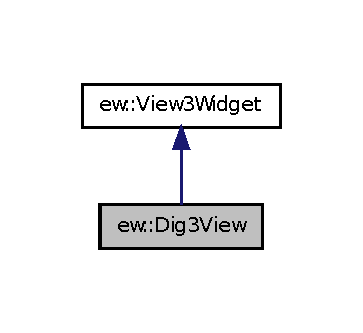
\includegraphics[width=174pt]{classew_1_1Dig3View__inherit__graph}
\end{center}
\end{figure}
\subsubsection*{Public Types}
\begin{DoxyCompactItemize}
\item 
enum \hyperlink{classew_1_1Dig3View_ac4e4e4036d49a73a3470f7c46057e13a}{item\_\-t} \{ \hyperlink{classew_1_1Dig3View_ac4e4e4036d49a73a3470f7c46057e13aa12554f487cbf4981a9cf8cf72a668bc7}{ITEM\_\-SLICE}, 
\hyperlink{classew_1_1Dig3View_ac4e4e4036d49a73a3470f7c46057e13aa19b28108a6c147a4f67a7ca301a4b9f4}{ITEM\_\-LANDMARKS}, 
\hyperlink{classew_1_1Dig3View_ac4e4e4036d49a73a3470f7c46057e13aa1921cd87bd7301098b2b318936a61beb}{ITEM\_\-CURVE}, 
\hyperlink{classew_1_1Dig3View_ac4e4e4036d49a73a3470f7c46057e13aaae05252997168fd1f936c7d04cfc57e5}{ITEM\_\-SURFACE}
 \}
\end{DoxyCompactItemize}
\subsubsection*{Public Member Functions}
\begin{DoxyCompactItemize}
\item 
\hyperlink{classew_1_1Dig3View_a50bf8f0ce6c29fa0f2a0e7f6bc7ba7bd}{Dig3View} (\hyperlink{classew_1_1Dig3}{ew::Dig3} $\ast$\hyperlink{classew_1_1Dig3View_af168346e6f66801de1d09ac262d55778}{dig3}, int space, int slice\_\-mode)
\item 
\hyperlink{classew_1_1Dig3View_a42119dd232d7912a3b2c5ac6bb1c2e59}{$\sim$Dig3View} ()
\item 
void \hyperlink{classew_1_1Dig3View_a5e4afce808324fc93b9c8dfb76c5e374}{set\_\-slice\_\-mode} (int sm)
\item 
int \hyperlink{classew_1_1Dig3View_a9f52b3a596a26a19e14ff3c14fecd8bb}{get\_\-slice\_\-mode} () const 
\item 
void \hyperlink{classew_1_1Dig3View_a2dd21d8d92c1e4fd3b6db3605a917208}{set\_\-space} (int sp)
\item 
int \hyperlink{classew_1_1Dig3View_ad22d8d32c11fa5e1300af7f193b08bbf}{get\_\-space} () const 
\item 
void \hyperlink{classew_1_1Dig3View_aa4ca632104fa5d74443e5444ffe6a353}{set\_\-link} (\hyperlink{classew_1_1Dig3View}{ew::Dig3View} $\ast$v, const \hyperlink{classew_1_1Transform3}{ew::Transform3} $\ast$tr)
\item 
void \hyperlink{classew_1_1Dig3View_a2a65eaef54bdbb099f038443779c932c}{set\_\-view\_\-mapping} (const \hyperlink{classew_1_1Transform3}{ew::Transform3} $\ast$tr)
\item 
void \hyperlink{classew_1_1Dig3View_aa90d11b918a9c0e27399acd495ecd669}{view\_\-post\_\-compose} (const \hyperlink{classew_1_1Transform3}{ew::Transform3} $\ast$tr)
\item 
\hyperlink{classew_1_1View3Image}{ew::View3Image} $\ast$const $\ast$ \hyperlink{classew_1_1Dig3View_af18fd260d6c6298c9472a7d52574560d}{get\_\-slice\_\-items} () const 
\item 
\hyperlink{classew_1_1View3Curve}{ew::View3Curve} $\ast$const $\ast$ \hyperlink{classew_1_1Dig3View_ad814bd3f449aec44fc66a6667c7766e9}{get\_\-curve\_\-items} () const 
\item 
\hyperlink{classew_1_1View3Surface}{ew::View3Surface} $\ast$const $\ast$ \hyperlink{classew_1_1Dig3View_aaa1719f8cfbf61e71c56b9a4af37e048}{get\_\-surface\_\-items} () const 
\item 
\hyperlink{classew_1_1View3Landmarks}{ew::View3Landmarks} $\ast$ \hyperlink{classew_1_1Dig3View_a669e570e748ac09e014ede10d82deaea}{get\_\-landmarks\_\-item} () const 
\item 
int \hyperlink{classew_1_1Dig3View_afda34fa72824b91563abe90e9736bfa5}{get\_\-index} () const 
\end{DoxyCompactItemize}
\subsubsection*{Public Attributes}
\begin{DoxyCompactItemize}
\item 
\hyperlink{classew_1_1Dig3}{ew::Dig3} $\ast$const \hyperlink{classew_1_1Dig3View_af168346e6f66801de1d09ac262d55778}{dig3}
\end{DoxyCompactItemize}


\subsubsection{Detailed Description}
\hyperlink{classew_1_1Dig3View}{ew::Dig3View} implements a view element of \hyperlink{classew_1_1Dig3}{ew::Dig3}.

\hyperlink{classew_1_1Dig3View}{ew::Dig3View} is a class without assignment or comparison. There are private member variables.

The settings and item settings of the base \hyperlink{classew_1_1View3Widget}{ew::View3Widget}, may be directly manipulated, except for the view mapping. The toolkit interaction of this widget should be handled by inheriting this class and implementing the pure virtual methods of \hyperlink{classew_1_1View3Widget}{ew::View3Widget}. 

\subsubsection{Member Enumeration Documentation}
\hypertarget{classew_1_1Dig3View_ac4e4e4036d49a73a3470f7c46057e13a}{
\index{ew::Dig3View@{ew::Dig3View}!item\_\-t@{item\_\-t}}
\index{item\_\-t@{item\_\-t}!ew::Dig3View@{ew::Dig3View}}
\paragraph[{item\_\-t}]{\setlength{\rightskip}{0pt plus 5cm}enum {\bf ew::Dig3View::item\_\-t}}\hfill}
\label{classew_1_1Dig3View_ac4e4e4036d49a73a3470f7c46057e13a}
These are the possible values for \hyperlink{classew_1_1View3Item_a7e21fcde8f082ba2409bcb2999a4b7fd}{ew::View3Item::type} for items created by this class. \begin{Desc}
\item[Enumerator: ]\par
\begin{description}
\index{ITEM\_\-SLICE@{ITEM\_\-SLICE}!ew::Dig3View@{ew::Dig3View}}\index{ew::Dig3View@{ew::Dig3View}!ITEM\_\-SLICE@{ITEM\_\-SLICE}}\item[{\em 
\hypertarget{classew_1_1Dig3View_ac4e4e4036d49a73a3470f7c46057e13aa12554f487cbf4981a9cf8cf72a668bc7}{
ITEM\_\-SLICE}
\label{classew_1_1Dig3View_ac4e4e4036d49a73a3470f7c46057e13aa12554f487cbf4981a9cf8cf72a668bc7}
}]Item that represents the primary slice. \index{ITEM\_\-LANDMARKS@{ITEM\_\-LANDMARKS}!ew::Dig3View@{ew::Dig3View}}\index{ew::Dig3View@{ew::Dig3View}!ITEM\_\-LANDMARKS@{ITEM\_\-LANDMARKS}}\item[{\em 
\hypertarget{classew_1_1Dig3View_ac4e4e4036d49a73a3470f7c46057e13aa19b28108a6c147a4f67a7ca301a4b9f4}{
ITEM\_\-LANDMARKS}
\label{classew_1_1Dig3View_ac4e4e4036d49a73a3470f7c46057e13aa19b28108a6c147a4f67a7ca301a4b9f4}
}]Item that represents form landmarks and semi-\/landmarks. \index{ITEM\_\-CURVE@{ITEM\_\-CURVE}!ew::Dig3View@{ew::Dig3View}}\index{ew::Dig3View@{ew::Dig3View}!ITEM\_\-CURVE@{ITEM\_\-CURVE}}\item[{\em 
\hypertarget{classew_1_1Dig3View_ac4e4e4036d49a73a3470f7c46057e13aa1921cd87bd7301098b2b318936a61beb}{
ITEM\_\-CURVE}
\label{classew_1_1Dig3View_ac4e4e4036d49a73a3470f7c46057e13aa1921cd87bd7301098b2b318936a61beb}
}]Item that represents form (note warped) curves. \index{ITEM\_\-SURFACE@{ITEM\_\-SURFACE}!ew::Dig3View@{ew::Dig3View}}\index{ew::Dig3View@{ew::Dig3View}!ITEM\_\-SURFACE@{ITEM\_\-SURFACE}}\item[{\em 
\hypertarget{classew_1_1Dig3View_ac4e4e4036d49a73a3470f7c46057e13aaae05252997168fd1f936c7d04cfc57e5}{
ITEM\_\-SURFACE}
\label{classew_1_1Dig3View_ac4e4e4036d49a73a3470f7c46057e13aaae05252997168fd1f936c7d04cfc57e5}
}]Item that represents form (note warped) surfaces. \end{description}
\end{Desc}



\subsubsection{Constructor \& Destructor Documentation}
\hypertarget{classew_1_1Dig3View_a50bf8f0ce6c29fa0f2a0e7f6bc7ba7bd}{
\index{ew::Dig3View@{ew::Dig3View}!Dig3View@{Dig3View}}
\index{Dig3View@{Dig3View}!ew::Dig3View@{ew::Dig3View}}
\paragraph[{Dig3View}]{\setlength{\rightskip}{0pt plus 5cm}ew::Dig3View::Dig3View (
\begin{DoxyParamCaption}
\item[{{\bf ew::Dig3} $\ast$}]{ dig3, }
\item[{int}]{ space, }
\item[{int}]{ slice\_\-mode}
\end{DoxyParamCaption}
)}\hfill}
\label{classew_1_1Dig3View_a50bf8f0ce6c29fa0f2a0e7f6bc7ba7bd}
This creates a view element of the {\itshape dig3\/}. 
\begin{DoxyParams}{Parameters}
\item[{\em dig3}]The \hyperlink{classew_1_1Dig3}{ew::Dig3} this view element will belong to. \item[{\em space}]Which space of the {\itshape dig3\/} this view element will initially display. Either 0 or 1. \item[{\em slice\_\-mode}]Whether this will be a slice view. Either 0 or 1. \end{DoxyParams}
\hypertarget{classew_1_1Dig3View_a42119dd232d7912a3b2c5ac6bb1c2e59}{
\index{ew::Dig3View@{ew::Dig3View}!$\sim$Dig3View@{$\sim$Dig3View}}
\index{$\sim$Dig3View@{$\sim$Dig3View}!ew::Dig3View@{ew::Dig3View}}
\paragraph[{$\sim$Dig3View}]{\setlength{\rightskip}{0pt plus 5cm}ew::Dig3View::$\sim$Dig3View (
\begin{DoxyParamCaption}
{}
\end{DoxyParamCaption}
)}\hfill}
\label{classew_1_1Dig3View_a42119dd232d7912a3b2c5ac6bb1c2e59}
This removes the view from \hyperlink{classew_1_1Dig3View_af168346e6f66801de1d09ac262d55778}{dig3}, and destroys it. 

\subsubsection{Member Function Documentation}
\hypertarget{classew_1_1Dig3View_a5e4afce808324fc93b9c8dfb76c5e374}{
\index{ew::Dig3View@{ew::Dig3View}!set\_\-slice\_\-mode@{set\_\-slice\_\-mode}}
\index{set\_\-slice\_\-mode@{set\_\-slice\_\-mode}!ew::Dig3View@{ew::Dig3View}}
\paragraph[{set\_\-slice\_\-mode}]{\setlength{\rightskip}{0pt plus 5cm}void ew::Dig3View::set\_\-slice\_\-mode (
\begin{DoxyParamCaption}
\item[{int}]{ sm}
\end{DoxyParamCaption}
)}\hfill}
\label{classew_1_1Dig3View_a5e4afce808324fc93b9c8dfb76c5e374}

\begin{DoxyParams}{Parameters}
\item[{\em sm}]Whether this view should now be a slice view. Either 0 or 1. \end{DoxyParams}
\hypertarget{classew_1_1Dig3View_a9f52b3a596a26a19e14ff3c14fecd8bb}{
\index{ew::Dig3View@{ew::Dig3View}!get\_\-slice\_\-mode@{get\_\-slice\_\-mode}}
\index{get\_\-slice\_\-mode@{get\_\-slice\_\-mode}!ew::Dig3View@{ew::Dig3View}}
\paragraph[{get\_\-slice\_\-mode}]{\setlength{\rightskip}{0pt plus 5cm}int ew::Dig3View::get\_\-slice\_\-mode (
\begin{DoxyParamCaption}
{}
\end{DoxyParamCaption}
) const\hspace{0.3cm}{\ttfamily  \mbox{[}inline\mbox{]}}}\hfill}
\label{classew_1_1Dig3View_a9f52b3a596a26a19e14ff3c14fecd8bb}
\begin{DoxyReturn}{Returns}
Whether this is a slice view. Either 0 or 1. 
\end{DoxyReturn}
\hypertarget{classew_1_1Dig3View_a2dd21d8d92c1e4fd3b6db3605a917208}{
\index{ew::Dig3View@{ew::Dig3View}!set\_\-space@{set\_\-space}}
\index{set\_\-space@{set\_\-space}!ew::Dig3View@{ew::Dig3View}}
\paragraph[{set\_\-space}]{\setlength{\rightskip}{0pt plus 5cm}void ew::Dig3View::set\_\-space (
\begin{DoxyParamCaption}
\item[{int}]{ sp}
\end{DoxyParamCaption}
)}\hfill}
\label{classew_1_1Dig3View_a2dd21d8d92c1e4fd3b6db3605a917208}

\begin{DoxyParams}{Parameters}
\item[{\em sp}]The index of the space this view should now be associated with. Either 0 or 1. \end{DoxyParams}
\hypertarget{classew_1_1Dig3View_ad22d8d32c11fa5e1300af7f193b08bbf}{
\index{ew::Dig3View@{ew::Dig3View}!get\_\-space@{get\_\-space}}
\index{get\_\-space@{get\_\-space}!ew::Dig3View@{ew::Dig3View}}
\paragraph[{get\_\-space}]{\setlength{\rightskip}{0pt plus 5cm}int ew::Dig3View::get\_\-space (
\begin{DoxyParamCaption}
{}
\end{DoxyParamCaption}
) const\hspace{0.3cm}{\ttfamily  \mbox{[}inline\mbox{]}}}\hfill}
\label{classew_1_1Dig3View_ad22d8d32c11fa5e1300af7f193b08bbf}
\begin{DoxyReturn}{Returns}
The index of the space this view is currently associated with. Either 0 or 1. 
\end{DoxyReturn}
\hypertarget{classew_1_1Dig3View_aa4ca632104fa5d74443e5444ffe6a353}{
\index{ew::Dig3View@{ew::Dig3View}!set\_\-link@{set\_\-link}}
\index{set\_\-link@{set\_\-link}!ew::Dig3View@{ew::Dig3View}}
\paragraph[{set\_\-link}]{\setlength{\rightskip}{0pt plus 5cm}void ew::Dig3View::set\_\-link (
\begin{DoxyParamCaption}
\item[{{\bf ew::Dig3View} $\ast$}]{ v, }
\item[{const {\bf ew::Transform3} $\ast$}]{ tr}
\end{DoxyParamCaption}
)}\hfill}
\label{classew_1_1Dig3View_aa4ca632104fa5d74443e5444ffe6a353}
This sets up a link between the view mapping of this view and of another one. Links must be disjoint cycles. The composition of the transforms should be the identity for sensible results. 
\begin{DoxyParams}{Parameters}
\item[{\em v}]The view to link to. \item[{\em tr}]The transform that should be left-\/composed with this view's view mapping to get the link views view mapping. \end{DoxyParams}
\hypertarget{classew_1_1Dig3View_a2a65eaef54bdbb099f038443779c932c}{
\index{ew::Dig3View@{ew::Dig3View}!set\_\-view\_\-mapping@{set\_\-view\_\-mapping}}
\index{set\_\-view\_\-mapping@{set\_\-view\_\-mapping}!ew::Dig3View@{ew::Dig3View}}
\paragraph[{set\_\-view\_\-mapping}]{\setlength{\rightskip}{0pt plus 5cm}void ew::Dig3View::set\_\-view\_\-mapping (
\begin{DoxyParamCaption}
\item[{const {\bf ew::Transform3} $\ast$}]{ tr}
\end{DoxyParamCaption}
)}\hfill}
\label{classew_1_1Dig3View_a2a65eaef54bdbb099f038443779c932c}
This operates on the view mapping of the base \hyperlink{classew_1_1View3Widget}{ew::View3Widget}, and synchronizes with other views and with slices as necessary. This method has the same name as a non-\/virtual method in the base class. 
\begin{DoxyParams}{Parameters}
\item[{\em tr}]As for \hyperlink{classew_1_1View3Widget_aca4dfffefdc6bf300e6f26ef76bb1913}{ew::View3Widget::set\_\-view\_\-mapping()}. \end{DoxyParams}


Reimplemented from \hyperlink{classew_1_1View3Widget_aca4dfffefdc6bf300e6f26ef76bb1913}{ew::View3Widget}.

\hypertarget{classew_1_1Dig3View_aa90d11b918a9c0e27399acd495ecd669}{
\index{ew::Dig3View@{ew::Dig3View}!view\_\-post\_\-compose@{view\_\-post\_\-compose}}
\index{view\_\-post\_\-compose@{view\_\-post\_\-compose}!ew::Dig3View@{ew::Dig3View}}
\paragraph[{view\_\-post\_\-compose}]{\setlength{\rightskip}{0pt plus 5cm}void ew::Dig3View::view\_\-post\_\-compose (
\begin{DoxyParamCaption}
\item[{const {\bf ew::Transform3} $\ast$}]{ tr}
\end{DoxyParamCaption}
)}\hfill}
\label{classew_1_1Dig3View_aa90d11b918a9c0e27399acd495ecd669}
This operates on the view mapping of the base \hyperlink{classew_1_1View3Widget}{ew::View3Widget}, and synchronizes with other views and with slices as necessary. This method has the same name as a non-\/virtual method in the base class. 
\begin{DoxyParams}{Parameters}
\item[{\em tr}]As for \hyperlink{classew_1_1View3Widget_a90e7e1db3ccb509999f68e3aa23d27f5}{ew::View3Widget::view\_\-post\_\-compose()}. \end{DoxyParams}


Reimplemented from \hyperlink{classew_1_1View3Widget_a90e7e1db3ccb509999f68e3aa23d27f5}{ew::View3Widget}.

\hypertarget{classew_1_1Dig3View_af18fd260d6c6298c9472a7d52574560d}{
\index{ew::Dig3View@{ew::Dig3View}!get\_\-slice\_\-items@{get\_\-slice\_\-items}}
\index{get\_\-slice\_\-items@{get\_\-slice\_\-items}!ew::Dig3View@{ew::Dig3View}}
\paragraph[{get\_\-slice\_\-items}]{\setlength{\rightskip}{0pt plus 5cm}{\bf ew::View3Image} $\ast$const $\ast$ ew::Dig3View::get\_\-slice\_\-items (
\begin{DoxyParamCaption}
{}
\end{DoxyParamCaption}
) const\hspace{0.3cm}{\ttfamily  \mbox{[}inline\mbox{]}}}\hfill}
\label{classew_1_1Dig3View_af18fd260d6c6298c9472a7d52574560d}
\begin{DoxyReturn}{Returns}
The slice item index. The i'th entry is the item displaying the slice of the i'th view of the \hyperlink{classew_1_1Dig3View_af168346e6f66801de1d09ac262d55778}{dig3}, or zero if the i'th view is not in slice mode, or is not associated with the same space. 
\end{DoxyReturn}
\hypertarget{classew_1_1Dig3View_ad814bd3f449aec44fc66a6667c7766e9}{
\index{ew::Dig3View@{ew::Dig3View}!get\_\-curve\_\-items@{get\_\-curve\_\-items}}
\index{get\_\-curve\_\-items@{get\_\-curve\_\-items}!ew::Dig3View@{ew::Dig3View}}
\paragraph[{get\_\-curve\_\-items}]{\setlength{\rightskip}{0pt plus 5cm}{\bf ew::View3Curve} $\ast$const $\ast$ ew::Dig3View::get\_\-curve\_\-items (
\begin{DoxyParamCaption}
{}
\end{DoxyParamCaption}
) const\hspace{0.3cm}{\ttfamily  \mbox{[}inline\mbox{]}}}\hfill}
\label{classew_1_1Dig3View_ad814bd3f449aec44fc66a6667c7766e9}
\begin{DoxyReturn}{Returns}
The curve item index. The i'th entry is the item displaying the i'th curve of the space this view is currently associated with. 
\end{DoxyReturn}
\hypertarget{classew_1_1Dig3View_aaa1719f8cfbf61e71c56b9a4af37e048}{
\index{ew::Dig3View@{ew::Dig3View}!get\_\-surface\_\-items@{get\_\-surface\_\-items}}
\index{get\_\-surface\_\-items@{get\_\-surface\_\-items}!ew::Dig3View@{ew::Dig3View}}
\paragraph[{get\_\-surface\_\-items}]{\setlength{\rightskip}{0pt plus 5cm}{\bf ew::View3Surface} $\ast$const $\ast$ ew::Dig3View::get\_\-surface\_\-items (
\begin{DoxyParamCaption}
{}
\end{DoxyParamCaption}
) const\hspace{0.3cm}{\ttfamily  \mbox{[}inline\mbox{]}}}\hfill}
\label{classew_1_1Dig3View_aaa1719f8cfbf61e71c56b9a4af37e048}
\begin{DoxyReturn}{Returns}
The surface item index. The i'th entry is the item displaying the i'th surface of the space this view is currently associated with. 
\end{DoxyReturn}
\hypertarget{classew_1_1Dig3View_a669e570e748ac09e014ede10d82deaea}{
\index{ew::Dig3View@{ew::Dig3View}!get\_\-landmarks\_\-item@{get\_\-landmarks\_\-item}}
\index{get\_\-landmarks\_\-item@{get\_\-landmarks\_\-item}!ew::Dig3View@{ew::Dig3View}}
\paragraph[{get\_\-landmarks\_\-item}]{\setlength{\rightskip}{0pt plus 5cm}{\bf ew::View3Landmarks} $\ast$ ew::Dig3View::get\_\-landmarks\_\-item (
\begin{DoxyParamCaption}
{}
\end{DoxyParamCaption}
) const\hspace{0.3cm}{\ttfamily  \mbox{[}inline\mbox{]}}}\hfill}
\label{classew_1_1Dig3View_a669e570e748ac09e014ede10d82deaea}
\begin{DoxyReturn}{Returns}
The landmarks item. 
\end{DoxyReturn}
\hypertarget{classew_1_1Dig3View_afda34fa72824b91563abe90e9736bfa5}{
\index{ew::Dig3View@{ew::Dig3View}!get\_\-index@{get\_\-index}}
\index{get\_\-index@{get\_\-index}!ew::Dig3View@{ew::Dig3View}}
\paragraph[{get\_\-index}]{\setlength{\rightskip}{0pt plus 5cm}int ew::Dig3View::get\_\-index (
\begin{DoxyParamCaption}
{}
\end{DoxyParamCaption}
) const\hspace{0.3cm}{\ttfamily  \mbox{[}inline\mbox{]}}}\hfill}
\label{classew_1_1Dig3View_afda34fa72824b91563abe90e9736bfa5}
\begin{DoxyReturn}{Returns}
The current index of this view element in the view index of \hyperlink{classew_1_1Dig3View_af168346e6f66801de1d09ac262d55778}{dig3}. 
\end{DoxyReturn}


\subsubsection{Member Data Documentation}
\hypertarget{classew_1_1Dig3View_af168346e6f66801de1d09ac262d55778}{
\index{ew::Dig3View@{ew::Dig3View}!dig3@{dig3}}
\index{dig3@{dig3}!ew::Dig3View@{ew::Dig3View}}
\paragraph[{dig3}]{\setlength{\rightskip}{0pt plus 5cm}{\bf ew::Dig3} $\ast$const {\bf ew::Dig3View::dig3}}\hfill}
\label{classew_1_1Dig3View_af168346e6f66801de1d09ac262d55778}
This points to the \hyperlink{classew_1_1Dig3}{ew::Dig3} that this \hyperlink{classew_1_1Dig3View}{ew::Dig3View} was created with. 
\hypertarget{classew_1_1ErrorIO}{
\subsection{ew::ErrorIO Class Reference}
\label{classew_1_1ErrorIO}\index{ew::ErrorIO@{ew::ErrorIO}}
}


I/O Exception.  




{\ttfamily \#include $<$ew/ErrorIO.h$>$}



Inherits std::runtime\_\-error.

\subsubsection*{Public Member Functions}
\begin{DoxyCompactItemize}
\item 
\hyperlink{classew_1_1ErrorIO_aba26a7556f22d4a8a4f588f9a44348c7}{ErrorIO} (const std::string \&desc)
\end{DoxyCompactItemize}


\subsubsection{Detailed Description}
\hyperlink{classew_1_1ErrorIO}{ew::ErrorIO} is an exception thrown by EW library classes to report input or output errors or bad file formats.

\hyperlink{classew_1_1ErrorIO}{ew::ErrorIO} is a trivial extension of std::runtime\_\-error. 

\subsubsection{Constructor \& Destructor Documentation}
\hypertarget{classew_1_1ErrorIO_aba26a7556f22d4a8a4f588f9a44348c7}{
\index{ew::ErrorIO@{ew::ErrorIO}!ErrorIO@{ErrorIO}}
\index{ErrorIO@{ErrorIO}!ew::ErrorIO@{ew::ErrorIO}}
\paragraph[{ErrorIO}]{\setlength{\rightskip}{0pt plus 5cm}ew::ErrorIO::ErrorIO (
\begin{DoxyParamCaption}
\item[{const std::string \&}]{ desc}
\end{DoxyParamCaption}
)\hspace{0.3cm}{\ttfamily  \mbox{[}explicit\mbox{]}}}\hfill}
\label{classew_1_1ErrorIO_aba26a7556f22d4a8a4f588f9a44348c7}
Construct an \hyperlink{classew_1_1ErrorIO}{ew::ErrorIO} object. 
\begin{DoxyParams}{Parameters}
\item[{\em desc}]the error description \end{DoxyParams}

\hypertarget{classew_1_1ErrorRuntime}{
\subsection{ew::ErrorRuntime Class Reference}
\label{classew_1_1ErrorRuntime}\index{ew::ErrorRuntime@{ew::ErrorRuntime}}
}


Runtime Exception.  




{\ttfamily \#include $<$ew/ErrorRuntime.h$>$}



Inherits std::runtime\_\-error.

\subsubsection*{Public Member Functions}
\begin{DoxyCompactItemize}
\item 
\hyperlink{classew_1_1ErrorRuntime_a553ea87aedbe17bbc8d984540fed0aec}{ErrorRuntime} (const std::string \&desc)
\end{DoxyCompactItemize}


\subsubsection{Detailed Description}
\hyperlink{classew_1_1ErrorRuntime}{ew::ErrorRuntime} is an exception thrown by EW library classes to report runtime errors.

\hyperlink{classew_1_1ErrorRuntime}{ew::ErrorRuntime} is a trivial extension of std::runtime\_\-error. 

\subsubsection{Constructor \& Destructor Documentation}
\hypertarget{classew_1_1ErrorRuntime_a553ea87aedbe17bbc8d984540fed0aec}{
\index{ew::ErrorRuntime@{ew::ErrorRuntime}!ErrorRuntime@{ErrorRuntime}}
\index{ErrorRuntime@{ErrorRuntime}!ew::ErrorRuntime@{ew::ErrorRuntime}}
\paragraph[{ErrorRuntime}]{\setlength{\rightskip}{0pt plus 5cm}ew::ErrorRuntime::ErrorRuntime (
\begin{DoxyParamCaption}
\item[{const std::string \&}]{ desc}
\end{DoxyParamCaption}
)\hspace{0.3cm}{\ttfamily  \mbox{[}explicit\mbox{]}}}\hfill}
\label{classew_1_1ErrorRuntime_a553ea87aedbe17bbc8d984540fed0aec}
Construct an EW::Error\_\-Runtime object. 
\begin{DoxyParams}{Parameters}
\item[{\em desc}]the error description \end{DoxyParams}

\hypertarget{classew_1_1Form3}{
\subsection{ew::Form3 Class Reference}
\label{classew_1_1Form3}\index{ew::Form3@{ew::Form3}}
}


Morphometric Form.  




{\ttfamily \#include $<$ew/Form3.h$>$}

\subsubsection*{Public Types}
\begin{DoxyCompactItemize}
\item 
enum \hyperlink{classew_1_1Form3_a0fb1f90f8936fc647de8bf351aa0f725}{state\_\-t} \{ \par
\hyperlink{classew_1_1Form3_a0fb1f90f8936fc647de8bf351aa0f725acce88d69a207a761cb9d267bf36a4882}{STATE\_\-SET}, 
\hyperlink{classew_1_1Form3_a0fb1f90f8936fc647de8bf351aa0f725afc4f92640e5a0ba7ba025265300df60d}{STATE\_\-UNSET}, 
\hyperlink{classew_1_1Form3_a0fb1f90f8936fc647de8bf351aa0f725a7c68944bfd7af307bf1097e3f6a98647}{STATE\_\-PROVISIONAL}, 
\hyperlink{classew_1_1Form3_a0fb1f90f8936fc647de8bf351aa0f725a929401893c671bbb4be2e50cba63949e}{STATE\_\-WARPED}, 
\par
\hyperlink{classew_1_1Form3_a0fb1f90f8936fc647de8bf351aa0f725accd0d7c17a3c1219c2c13d0d25af018c}{STATE\_\-PROJECTED}, 
\hyperlink{classew_1_1Form3_a0fb1f90f8936fc647de8bf351aa0f725a845f0d997e74de0ec5a055f923ef6975}{STATE\_\-OPTIMIZED}
 \}
\item 
enum \hyperlink{classew_1_1Form3_abfa10aaae60c2888a7e201cd8fd45733}{point\_\-t} \{ \par
\hyperlink{classew_1_1Form3_abfa10aaae60c2888a7e201cd8fd45733aafd3312606d8242fd8a650020fb682c5}{TYPE\_\-LANDMARK}, 
\hyperlink{classew_1_1Form3_abfa10aaae60c2888a7e201cd8fd45733a2ebb795c7e887f4d69bae678ad490df6}{TYPE\_\-SEMI\_\-LANDMARK}, 
\hyperlink{classew_1_1Form3_abfa10aaae60c2888a7e201cd8fd45733a63adf7483ccd80afe7d295aecf1508c0}{TYPE\_\-POINT}, 
\hyperlink{classew_1_1Form3_abfa10aaae60c2888a7e201cd8fd45733af4a3d6f8994ebe1d4ee511fdf4ba6da0}{TYPE\_\-LINE}, 
\par
\hyperlink{classew_1_1Form3_abfa10aaae60c2888a7e201cd8fd45733a7d720e976a12e6140d954e3dfbcfeb2f}{TYPE\_\-PLANE}, 
\hyperlink{classew_1_1Form3_abfa10aaae60c2888a7e201cd8fd45733a03680acbf4911849a3fbdfa9c310f787}{TYPE\_\-FRAME}
 \}
\end{DoxyCompactItemize}
\subsubsection*{Public Member Functions}
\begin{DoxyCompactItemize}
\item 
void \hyperlink{classew_1_1Form3_a142e4923377ce451364f9c902713372c}{reset} ()
\item 
void \hyperlink{classew_1_1Form3_a9de2d04fa5fd964de69951339ed9c1cf}{read\_\-file} (const char $\ast$file)
\item 
void \hyperlink{classew_1_1Form3_ab5abad2f912616bc7d0a1e3dd37943bb}{write\_\-file} (const char $\ast$file, bool compress) const 
\item 
bool \hyperlink{classew_1_1Form3_ad3f7f4ab0210f7753dc42df94fec817d}{search\_\-volume} (int $\ast$position, const char $\ast$id) const 
\item 
bool \hyperlink{classew_1_1Form3_a863b953b1d79be8c29406cde111b4d6e}{search\_\-surface} (int $\ast$position, const char $\ast$id) const 
\item 
bool \hyperlink{classew_1_1Form3_acef9a7cb9f65ccc4a7ed70c9968441ca}{search\_\-curve} (int $\ast$position, const char $\ast$id) const 
\item 
bool \hyperlink{classew_1_1Form3_a1da8c7154ae6a6bbe904034c9fdbb8df}{search\_\-pointset} (int $\ast$position, const char $\ast$id) const 
\item 
bool \hyperlink{classew_1_1Form3_ac2ce9094d917d97a7424edae355c8328}{search\_\-embedding} (int $\ast$position, const char $\ast$id1, const char $\ast$id2) const 
\item 
bool \hyperlink{classew_1_1Form3_a593bc0c4f71b5f24afee1d55ac07302e}{search\_\-reflection} (int $\ast$position, const char $\ast$id1, const char $\ast$id2) const 
\item 
const char $\ast$ \hyperlink{classew_1_1Form3_a7fa5b81fa3813eb833155e3d5cb7e2f3}{search\_\-superset} (const char $\ast$id) const 
\item 
void \hyperlink{classew_1_1Form3_a0918a426ed95d3244d8212dc985d0897}{set\_\-superset} (const char $\ast$subset\_\-id, const char $\ast$superset\_\-id)
\item 
void \hyperlink{classew_1_1Form3_ae15e78e95043b8e7f196a32e7d4527a6}{swap} (\hyperlink{classew_1_1Form3}{ew::Form3} \&f)
\item 
bool \hyperlink{classew_1_1Form3_a7704ee4daef7adf30a0199756b2fcc22}{operator==} (const \hyperlink{classew_1_1Form3}{ew::Form3} \&a) const 
\item 
bool \hyperlink{classew_1_1Form3_a002e398fca7517dfacc077a1450190d0}{operator!=} (const \hyperlink{classew_1_1Form3}{ew::Form3} \&a) const 
\end{DoxyCompactItemize}
\subsubsection*{Public Attributes}
\begin{DoxyCompactItemize}
\item 
std::vector$<$ \hyperlink{classew_1_1Form3Volume}{ew::Form3Volume} $>$ \hyperlink{classew_1_1Form3_aab5dcd7658c84512d05e095e58341fa7}{volumes}
\item 
std::vector$<$ \hyperlink{classew_1_1Form3Surface}{ew::Form3Surface} $>$ \hyperlink{classew_1_1Form3_abd4405612b484b5d9d87b643d316b020}{surfaces}
\item 
std::vector$<$ \hyperlink{classew_1_1Form3Curve}{ew::Form3Curve} $>$ \hyperlink{classew_1_1Form3_ab60def495fb8fea585dff2fb8c94d845}{curves}
\item 
std::vector$<$ \hyperlink{classew_1_1Form3PointSet}{ew::Form3PointSet} $>$ \hyperlink{classew_1_1Form3_aed0e94682a4de9b871c8fb15906bcc09}{pointsets}
\item 
std::vector$<$ \hyperlink{classew_1_1Form3Embedding}{ew::Form3Embedding} $>$ \hyperlink{classew_1_1Form3_a05ace76e2206ea825495538e93d9ba4c}{embeddings}
\item 
std::vector$<$ \hyperlink{classew_1_1Form3Reflection}{ew::Form3Reflection} $>$ \hyperlink{classew_1_1Form3_a4df1d049f2c5ca83f194d4ac9cf9f074}{reflections}
\end{DoxyCompactItemize}


\subsubsection{Detailed Description}
\hyperlink{classew_1_1Form3}{ew::Form3} represents morphometric forms in $\mathbb{R}^3$. These are landmark configurations, possibly including semi-\/landmarks, generalized to include curve, surface and volume data.

\hyperlink{classew_1_1Form3}{ew::Form3} is a data structure that supports default construction, copy construction, assignment and equality comparison.

\hyperlink{classew_1_1Form3}{ew::Form3} data is represented in form files read by \hyperlink{classew_1_1Form3_a9de2d04fa5fd964de69951339ed9c1cf}{read\_\-file} and written by \hyperlink{classew_1_1Form3_ab5abad2f912616bc7d0a1e3dd37943bb}{write\_\-file}. These are example files:
\begin{DoxyItemize}
\item \hyperlink{simple_landmarks_8form}{simple\_\-landmarks.form}
\item \hyperlink{mandible_template_8form}{mandible\_\-landmarks.form}
\item \hyperlink{mandible_case_8form}{mandible\_\-case.form}
\end{DoxyItemize}The representation is exact except that filenames in the form files are abbreviated to relative filenames in common situations were possible, but in \hyperlink{classew_1_1Form3}{ew::Form3} they are always in canonical form.

All elements in the form have an id. These id's must be unique in the from. 

\subsubsection{Member Enumeration Documentation}
\hypertarget{classew_1_1Form3_a0fb1f90f8936fc647de8bf351aa0f725}{
\index{ew::Form3@{ew::Form3}!state\_\-t@{state\_\-t}}
\index{state\_\-t@{state\_\-t}!ew::Form3@{ew::Form3}}
\paragraph[{state\_\-t}]{\setlength{\rightskip}{0pt plus 5cm}enum {\bf ew::Form3::state\_\-t}}\hfill}
\label{classew_1_1Form3_a0fb1f90f8936fc647de8bf351aa0f725}
Some elements can have a state associated with them. These are the possible values. Not all states are appropriate for all element types. The default is \hyperlink{classew_1_1Form3_a0fb1f90f8936fc647de8bf351aa0f725acce88d69a207a761cb9d267bf36a4882}{STATE\_\-SET}. \begin{Desc}
\item[Enumerator: ]\par
\begin{description}
\index{STATE\_\-SET@{STATE\_\-SET}!ew::Form3@{ew::Form3}}\index{ew::Form3@{ew::Form3}!STATE\_\-SET@{STATE\_\-SET}}\item[{\em 
\hypertarget{classew_1_1Form3_a0fb1f90f8936fc647de8bf351aa0f725acce88d69a207a761cb9d267bf36a4882}{
STATE\_\-SET}
\label{classew_1_1Form3_a0fb1f90f8936fc647de8bf351aa0f725acce88d69a207a761cb9d267bf36a4882}
}]The element has been explicitly digitized (default). \index{STATE\_\-UNSET@{STATE\_\-UNSET}!ew::Form3@{ew::Form3}}\index{ew::Form3@{ew::Form3}!STATE\_\-UNSET@{STATE\_\-UNSET}}\item[{\em 
\hypertarget{classew_1_1Form3_a0fb1f90f8936fc647de8bf351aa0f725afc4f92640e5a0ba7ba025265300df60d}{
STATE\_\-UNSET}
\label{classew_1_1Form3_a0fb1f90f8936fc647de8bf351aa0f725afc4f92640e5a0ba7ba025265300df60d}
}]The element has not been digitized. \index{STATE\_\-PROVISIONAL@{STATE\_\-PROVISIONAL}!ew::Form3@{ew::Form3}}\index{ew::Form3@{ew::Form3}!STATE\_\-PROVISIONAL@{STATE\_\-PROVISIONAL}}\item[{\em 
\hypertarget{classew_1_1Form3_a0fb1f90f8936fc647de8bf351aa0f725a7c68944bfd7af307bf1097e3f6a98647}{
STATE\_\-PROVISIONAL}
\label{classew_1_1Form3_a0fb1f90f8936fc647de8bf351aa0f725a7c68944bfd7af307bf1097e3f6a98647}
}]The element has been provisionally digitized. \index{STATE\_\-WARPED@{STATE\_\-WARPED}!ew::Form3@{ew::Form3}}\index{ew::Form3@{ew::Form3}!STATE\_\-WARPED@{STATE\_\-WARPED}}\item[{\em 
\hypertarget{classew_1_1Form3_a0fb1f90f8936fc647de8bf351aa0f725a929401893c671bbb4be2e50cba63949e}{
STATE\_\-WARPED}
\label{classew_1_1Form3_a0fb1f90f8936fc647de8bf351aa0f725a929401893c671bbb4be2e50cba63949e}
}]The element is the image under a warp. \index{STATE\_\-PROJECTED@{STATE\_\-PROJECTED}!ew::Form3@{ew::Form3}}\index{ew::Form3@{ew::Form3}!STATE\_\-PROJECTED@{STATE\_\-PROJECTED}}\item[{\em 
\hypertarget{classew_1_1Form3_a0fb1f90f8936fc647de8bf351aa0f725accd0d7c17a3c1219c2c13d0d25af018c}{
STATE\_\-PROJECTED}
\label{classew_1_1Form3_a0fb1f90f8936fc647de8bf351aa0f725accd0d7c17a3c1219c2c13d0d25af018c}
}]The element has been projected. \index{STATE\_\-OPTIMIZED@{STATE\_\-OPTIMIZED}!ew::Form3@{ew::Form3}}\index{ew::Form3@{ew::Form3}!STATE\_\-OPTIMIZED@{STATE\_\-OPTIMIZED}}\item[{\em 
\hypertarget{classew_1_1Form3_a0fb1f90f8936fc647de8bf351aa0f725a845f0d997e74de0ec5a055f923ef6975}{
STATE\_\-OPTIMIZED}
\label{classew_1_1Form3_a0fb1f90f8936fc647de8bf351aa0f725a845f0d997e74de0ec5a055f923ef6975}
}]The element has been optimized. \end{description}
\end{Desc}

\hypertarget{classew_1_1Form3_abfa10aaae60c2888a7e201cd8fd45733}{
\index{ew::Form3@{ew::Form3}!point\_\-t@{point\_\-t}}
\index{point\_\-t@{point\_\-t}!ew::Form3@{ew::Form3}}
\paragraph[{point\_\-t}]{\setlength{\rightskip}{0pt plus 5cm}enum {\bf ew::Form3::point\_\-t}}\hfill}
\label{classew_1_1Form3_abfa10aaae60c2888a7e201cd8fd45733}
Point sets can have different types. These are the possible values. The default is \hyperlink{classew_1_1Form3_abfa10aaae60c2888a7e201cd8fd45733aafd3312606d8242fd8a650020fb682c5}{TYPE\_\-LANDMARK}. \begin{Desc}
\item[Enumerator: ]\par
\begin{description}
\index{TYPE\_\-LANDMARK@{TYPE\_\-LANDMARK}!ew::Form3@{ew::Form3}}\index{ew::Form3@{ew::Form3}!TYPE\_\-LANDMARK@{TYPE\_\-LANDMARK}}\item[{\em 
\hypertarget{classew_1_1Form3_abfa10aaae60c2888a7e201cd8fd45733aafd3312606d8242fd8a650020fb682c5}{
TYPE\_\-LANDMARK}
\label{classew_1_1Form3_abfa10aaae60c2888a7e201cd8fd45733aafd3312606d8242fd8a650020fb682c5}
}]The points are landmarks (default). \index{TYPE\_\-SEMI\_\-LANDMARK@{TYPE\_\-SEMI\_\-LANDMARK}!ew::Form3@{ew::Form3}}\index{ew::Form3@{ew::Form3}!TYPE\_\-SEMI\_\-LANDMARK@{TYPE\_\-SEMI\_\-LANDMARK}}\item[{\em 
\hypertarget{classew_1_1Form3_abfa10aaae60c2888a7e201cd8fd45733a2ebb795c7e887f4d69bae678ad490df6}{
TYPE\_\-SEMI\_\-LANDMARK}
\label{classew_1_1Form3_abfa10aaae60c2888a7e201cd8fd45733a2ebb795c7e887f4d69bae678ad490df6}
}]The points are semi-\/landmarks. \index{TYPE\_\-POINT@{TYPE\_\-POINT}!ew::Form3@{ew::Form3}}\index{ew::Form3@{ew::Form3}!TYPE\_\-POINT@{TYPE\_\-POINT}}\item[{\em 
\hypertarget{classew_1_1Form3_abfa10aaae60c2888a7e201cd8fd45733a63adf7483ccd80afe7d295aecf1508c0}{
TYPE\_\-POINT}
\label{classew_1_1Form3_abfa10aaae60c2888a7e201cd8fd45733a63adf7483ccd80afe7d295aecf1508c0}
}]The point is a non-\/landmark point. \index{TYPE\_\-LINE@{TYPE\_\-LINE}!ew::Form3@{ew::Form3}}\index{ew::Form3@{ew::Form3}!TYPE\_\-LINE@{TYPE\_\-LINE}}\item[{\em 
\hypertarget{classew_1_1Form3_abfa10aaae60c2888a7e201cd8fd45733af4a3d6f8994ebe1d4ee511fdf4ba6da0}{
TYPE\_\-LINE}
\label{classew_1_1Form3_abfa10aaae60c2888a7e201cd8fd45733af4a3d6f8994ebe1d4ee511fdf4ba6da0}
}]The point represents a line, such as a best-\/fit axis of symmetry. \index{TYPE\_\-PLANE@{TYPE\_\-PLANE}!ew::Form3@{ew::Form3}}\index{ew::Form3@{ew::Form3}!TYPE\_\-PLANE@{TYPE\_\-PLANE}}\item[{\em 
\hypertarget{classew_1_1Form3_abfa10aaae60c2888a7e201cd8fd45733a7d720e976a12e6140d954e3dfbcfeb2f}{
TYPE\_\-PLANE}
\label{classew_1_1Form3_abfa10aaae60c2888a7e201cd8fd45733a7d720e976a12e6140d954e3dfbcfeb2f}
}]The point represents a plane, such as a best-\/fit multi-\/tangent or best-\/fit symmetry plane. \index{TYPE\_\-FRAME@{TYPE\_\-FRAME}!ew::Form3@{ew::Form3}}\index{ew::Form3@{ew::Form3}!TYPE\_\-FRAME@{TYPE\_\-FRAME}}\item[{\em 
\hypertarget{classew_1_1Form3_abfa10aaae60c2888a7e201cd8fd45733a03680acbf4911849a3fbdfa9c310f787}{
TYPE\_\-FRAME}
\label{classew_1_1Form3_abfa10aaae60c2888a7e201cd8fd45733a03680acbf4911849a3fbdfa9c310f787}
}]The point represents a frame, such as a standard view. \end{description}
\end{Desc}



\subsubsection{Member Function Documentation}
\hypertarget{classew_1_1Form3_a142e4923377ce451364f9c902713372c}{
\index{ew::Form3@{ew::Form3}!reset@{reset}}
\index{reset@{reset}!ew::Form3@{ew::Form3}}
\paragraph[{reset}]{\setlength{\rightskip}{0pt plus 5cm}void ew::Form3::reset (
\begin{DoxyParamCaption}
{}
\end{DoxyParamCaption}
)}\hfill}
\label{classew_1_1Form3_a142e4923377ce451364f9c902713372c}
This resets the form to its initial state. \hypertarget{classew_1_1Form3_a9de2d04fa5fd964de69951339ed9c1cf}{
\index{ew::Form3@{ew::Form3}!read\_\-file@{read\_\-file}}
\index{read\_\-file@{read\_\-file}!ew::Form3@{ew::Form3}}
\paragraph[{read\_\-file}]{\setlength{\rightskip}{0pt plus 5cm}void ew::Form3::read\_\-file (
\begin{DoxyParamCaption}
\item[{const char $\ast$}]{ file}
\end{DoxyParamCaption}
)}\hfill}
\label{classew_1_1Form3_a9de2d04fa5fd964de69951339ed9c1cf}
This reads a form from a file. The file must be a real filename, URL's are not supported. The file can be compressed with gzip compression. Relative filenames with initial path component \char`\"{}.\char`\"{} inside the file are converted to canonical filenames using the directory part of {\itshape file\/}. If an exception is thrown, the form is unchanged. 
\begin{DoxyParams}{Parameters}
\item[{\em file}]The canonical name of the file to read. \end{DoxyParams}

\begin{DoxyExceptions}{Exceptions}
\item[{\em std::bad\_\-alloc}]\item[{\em \hyperlink{classew_1_1ErrorIO}{ew::ErrorIO}}]\end{DoxyExceptions}
\hypertarget{classew_1_1Form3_ab5abad2f912616bc7d0a1e3dd37943bb}{
\index{ew::Form3@{ew::Form3}!write\_\-file@{write\_\-file}}
\index{write\_\-file@{write\_\-file}!ew::Form3@{ew::Form3}}
\paragraph[{write\_\-file}]{\setlength{\rightskip}{0pt plus 5cm}void ew::Form3::write\_\-file (
\begin{DoxyParamCaption}
\item[{const char $\ast$}]{ file, }
\item[{bool}]{ compress}
\end{DoxyParamCaption}
) const}\hfill}
\label{classew_1_1Form3_ab5abad2f912616bc7d0a1e3dd37943bb}
This writes a form to a file. Filenames written into the output are converted to relative filenames with initial path component \char`\"{}.\char`\"{} if their path contains the directory part of {\itshape file\/} as an initial segment. 
\begin{DoxyParams}{Parameters}
\item[{\em file}]The canonical name of the file to write. \item[{\em compress}]If {\ttfamily true}, write the file compressed with gzip compression. \end{DoxyParams}

\begin{DoxyExceptions}{Exceptions}
\item[{\em std::bad\_\-alloc}]\item[{\em \hyperlink{classew_1_1ErrorIO}{ew::ErrorIO}}]\end{DoxyExceptions}
\hypertarget{classew_1_1Form3_ad3f7f4ab0210f7753dc42df94fec817d}{
\index{ew::Form3@{ew::Form3}!search\_\-volume@{search\_\-volume}}
\index{search\_\-volume@{search\_\-volume}!ew::Form3@{ew::Form3}}
\paragraph[{search\_\-volume}]{\setlength{\rightskip}{0pt plus 5cm}bool ew::Form3::search\_\-volume (
\begin{DoxyParamCaption}
\item[{int $\ast$}]{ position, }
\item[{const char $\ast$}]{ id}
\end{DoxyParamCaption}
) const}\hfill}
\label{classew_1_1Form3_ad3f7f4ab0210f7753dc42df94fec817d}
This searches the volumes in the form for an id. 
\begin{DoxyParams}{Parameters}
\item[\mbox{\tt[out]} {\em position}]The index in the vector that a volume with this id would be if inserted into the vector of volumes. \item[{\em id}]The id to search for. \end{DoxyParams}
\begin{DoxyReturn}{Returns}
{\ttfamily true} if the id is an existing volume id. 
\end{DoxyReturn}
\hypertarget{classew_1_1Form3_a863b953b1d79be8c29406cde111b4d6e}{
\index{ew::Form3@{ew::Form3}!search\_\-surface@{search\_\-surface}}
\index{search\_\-surface@{search\_\-surface}!ew::Form3@{ew::Form3}}
\paragraph[{search\_\-surface}]{\setlength{\rightskip}{0pt plus 5cm}bool ew::Form3::search\_\-surface (
\begin{DoxyParamCaption}
\item[{int $\ast$}]{ position, }
\item[{const char $\ast$}]{ id}
\end{DoxyParamCaption}
) const}\hfill}
\label{classew_1_1Form3_a863b953b1d79be8c29406cde111b4d6e}
This searches the surfaces in the form for an id. 
\begin{DoxyParams}{Parameters}
\item[\mbox{\tt[out]} {\em position}]The index in the vector that a surface with this id would be if inserted into the vector of surfaces. \item[{\em id}]The id to search for. \end{DoxyParams}
\begin{DoxyReturn}{Returns}
{\ttfamily true} if the id is an existing surface id. 
\end{DoxyReturn}
\hypertarget{classew_1_1Form3_acef9a7cb9f65ccc4a7ed70c9968441ca}{
\index{ew::Form3@{ew::Form3}!search\_\-curve@{search\_\-curve}}
\index{search\_\-curve@{search\_\-curve}!ew::Form3@{ew::Form3}}
\paragraph[{search\_\-curve}]{\setlength{\rightskip}{0pt plus 5cm}bool ew::Form3::search\_\-curve (
\begin{DoxyParamCaption}
\item[{int $\ast$}]{ position, }
\item[{const char $\ast$}]{ id}
\end{DoxyParamCaption}
) const}\hfill}
\label{classew_1_1Form3_acef9a7cb9f65ccc4a7ed70c9968441ca}
This searches the curves in the form for an id. 
\begin{DoxyParams}{Parameters}
\item[\mbox{\tt[out]} {\em position}]The index in the vector that a curve with this id would be if inserted into the vector of curves. \item[{\em id}]The id to search for. \end{DoxyParams}
\begin{DoxyReturn}{Returns}
{\ttfamily true} if the id is an existing curve id. 
\end{DoxyReturn}
\hypertarget{classew_1_1Form3_a1da8c7154ae6a6bbe904034c9fdbb8df}{
\index{ew::Form3@{ew::Form3}!search\_\-pointset@{search\_\-pointset}}
\index{search\_\-pointset@{search\_\-pointset}!ew::Form3@{ew::Form3}}
\paragraph[{search\_\-pointset}]{\setlength{\rightskip}{0pt plus 5cm}bool ew::Form3::search\_\-pointset (
\begin{DoxyParamCaption}
\item[{int $\ast$}]{ position, }
\item[{const char $\ast$}]{ id}
\end{DoxyParamCaption}
) const}\hfill}
\label{classew_1_1Form3_a1da8c7154ae6a6bbe904034c9fdbb8df}
This searches the point sets in the form for an id. 
\begin{DoxyParams}{Parameters}
\item[\mbox{\tt[out]} {\em position}]The index in the vector that a point set with this id would be if inserted into the vector of point sets. \item[{\em id}]The id to search for. \end{DoxyParams}
\begin{DoxyReturn}{Returns}
{\ttfamily true} if the id is an existing point set id. 
\end{DoxyReturn}
\hypertarget{classew_1_1Form3_ac2ce9094d917d97a7424edae355c8328}{
\index{ew::Form3@{ew::Form3}!search\_\-embedding@{search\_\-embedding}}
\index{search\_\-embedding@{search\_\-embedding}!ew::Form3@{ew::Form3}}
\paragraph[{search\_\-embedding}]{\setlength{\rightskip}{0pt plus 5cm}bool ew::Form3::search\_\-embedding (
\begin{DoxyParamCaption}
\item[{int $\ast$}]{ position, }
\item[{const char $\ast$}]{ id1, }
\item[{const char $\ast$}]{ id2}
\end{DoxyParamCaption}
) const}\hfill}
\label{classew_1_1Form3_ac2ce9094d917d97a7424edae355c8328}
This searches the embeddings in the form for the id's. 
\begin{DoxyParams}{Parameters}
\item[\mbox{\tt[out]} {\em position}]The index in the vector that a embedding with these id's would be if inserted into the vector of embeddings. \item[{\em id1}]The subset\_\-id to search for. \item[{\em id2}]The superset\_\-id to search for. \end{DoxyParams}
\begin{DoxyReturn}{Returns}
{\ttfamily true} if the id's belong to an existing embedding. 
\end{DoxyReturn}
\hypertarget{classew_1_1Form3_a593bc0c4f71b5f24afee1d55ac07302e}{
\index{ew::Form3@{ew::Form3}!search\_\-reflection@{search\_\-reflection}}
\index{search\_\-reflection@{search\_\-reflection}!ew::Form3@{ew::Form3}}
\paragraph[{search\_\-reflection}]{\setlength{\rightskip}{0pt plus 5cm}bool ew::Form3::search\_\-reflection (
\begin{DoxyParamCaption}
\item[{int $\ast$}]{ position, }
\item[{const char $\ast$}]{ id1, }
\item[{const char $\ast$}]{ id2}
\end{DoxyParamCaption}
) const}\hfill}
\label{classew_1_1Form3_a593bc0c4f71b5f24afee1d55ac07302e}
This searches the reflections in the form for the id's. 
\begin{DoxyParams}{Parameters}
\item[\mbox{\tt[out]} {\em position}]The index in the vector that a reflection with these id's would be if inserted into the vector of reflections. \item[{\em id1}]The left\_\-id to search for. \item[{\em id2}]The right\_\-id to search for. \end{DoxyParams}
\begin{DoxyReturn}{Returns}
{\ttfamily true} if the id's belong to an existing reflection. 
\end{DoxyReturn}
\hypertarget{classew_1_1Form3_a7fa5b81fa3813eb833155e3d5cb7e2f3}{
\index{ew::Form3@{ew::Form3}!search\_\-superset@{search\_\-superset}}
\index{search\_\-superset@{search\_\-superset}!ew::Form3@{ew::Form3}}
\paragraph[{search\_\-superset}]{\setlength{\rightskip}{0pt plus 5cm}const char $\ast$ ew::Form3::search\_\-superset (
\begin{DoxyParamCaption}
\item[{const char $\ast$}]{ id}
\end{DoxyParamCaption}
) const}\hfill}
\label{classew_1_1Form3_a7fa5b81fa3813eb833155e3d5cb7e2f3}
This searches the embedding relations to see what, if any, element is a unique superset of a given element. 
\begin{DoxyParams}{Parameters}
\item[\mbox{\tt[in]} {\em id}]The id of the original element. \end{DoxyParams}
\begin{DoxyReturn}{Returns}
The id of the unique superset of the original element, or 0. This pointer is valid until the form is changed. 
\end{DoxyReturn}
\hypertarget{classew_1_1Form3_a0918a426ed95d3244d8212dc985d0897}{
\index{ew::Form3@{ew::Form3}!set\_\-superset@{set\_\-superset}}
\index{set\_\-superset@{set\_\-superset}!ew::Form3@{ew::Form3}}
\paragraph[{set\_\-superset}]{\setlength{\rightskip}{0pt plus 5cm}void ew::Form3::set\_\-superset (
\begin{DoxyParamCaption}
\item[{const char $\ast$}]{ subset\_\-id, }
\item[{const char $\ast$}]{ superset\_\-id}
\end{DoxyParamCaption}
)}\hfill}
\label{classew_1_1Form3_a0918a426ed95d3244d8212dc985d0897}
This makes one element the unique superset of another element. 
\begin{DoxyParams}{Parameters}
\item[{\em subset\_\-id}]The id of the element that should have a unique superset. \item[{\em superset\_\-id}]The id of the element that be the unique superset. \end{DoxyParams}
\hypertarget{classew_1_1Form3_ae15e78e95043b8e7f196a32e7d4527a6}{
\index{ew::Form3@{ew::Form3}!swap@{swap}}
\index{swap@{swap}!ew::Form3@{ew::Form3}}
\paragraph[{swap}]{\setlength{\rightskip}{0pt plus 5cm}void ew::Form3::swap (
\begin{DoxyParamCaption}
\item[{{\bf ew::Form3} \&}]{ that}
\end{DoxyParamCaption}
)\hspace{0.3cm}{\ttfamily  \mbox{[}inline\mbox{]}}}\hfill}
\label{classew_1_1Form3_ae15e78e95043b8e7f196a32e7d4527a6}
This swaps the data of 2 forms without any copying. 
\begin{DoxyParams}{Parameters}
\item[{\em that}]The form to swap with {\ttfamily this}. \end{DoxyParams}
\hypertarget{classew_1_1Form3_a7704ee4daef7adf30a0199756b2fcc22}{
\index{ew::Form3@{ew::Form3}!operator==@{operator==}}
\index{operator==@{operator==}!ew::Form3@{ew::Form3}}
\paragraph[{operator==}]{\setlength{\rightskip}{0pt plus 5cm}bool ew::Form3::operator== (
\begin{DoxyParamCaption}
\item[{const {\bf ew::Form3} \&}]{ a}
\end{DoxyParamCaption}
) const}\hfill}
\label{classew_1_1Form3_a7704ee4daef7adf30a0199756b2fcc22}
Compares this form with another, member by member. 
\begin{DoxyParams}{Parameters}
\item[{\em a}]the other form \end{DoxyParams}
\hypertarget{classew_1_1Form3_a002e398fca7517dfacc077a1450190d0}{
\index{ew::Form3@{ew::Form3}!operator!=@{operator!=}}
\index{operator!=@{operator!=}!ew::Form3@{ew::Form3}}
\paragraph[{operator!=}]{\setlength{\rightskip}{0pt plus 5cm}bool ew::Form3::operator!= (
\begin{DoxyParamCaption}
\item[{const {\bf ew::Form3} \&}]{ a}
\end{DoxyParamCaption}
) const\hspace{0.3cm}{\ttfamily  \mbox{[}inline\mbox{]}}}\hfill}
\label{classew_1_1Form3_a002e398fca7517dfacc077a1450190d0}
Compares this form with another, member by member. 
\begin{DoxyParams}{Parameters}
\item[{\em a}]the other form \end{DoxyParams}


\subsubsection{Member Data Documentation}
\hypertarget{classew_1_1Form3_aab5dcd7658c84512d05e095e58341fa7}{
\index{ew::Form3@{ew::Form3}!volumes@{volumes}}
\index{volumes@{volumes}!ew::Form3@{ew::Form3}}
\paragraph[{volumes}]{\setlength{\rightskip}{0pt plus 5cm}std::vector$<$ {\bf ew::Form3Volume} $>$ {\bf ew::Form3::volumes}}\hfill}
\label{classew_1_1Form3_aab5dcd7658c84512d05e095e58341fa7}
An arbitrary number of volume elements. The volume data is stored in separate files. The files named are not expected to change during their use. These must be in alphabetical order by \hyperlink{classew_1_1Form3Volume_aede415929600c673c12b8d99f600ea37}{ew::Form3Volume::id} in the POSIX sorting order. \hypertarget{classew_1_1Form3_abd4405612b484b5d9d87b643d316b020}{
\index{ew::Form3@{ew::Form3}!surfaces@{surfaces}}
\index{surfaces@{surfaces}!ew::Form3@{ew::Form3}}
\paragraph[{surfaces}]{\setlength{\rightskip}{0pt plus 5cm}std::vector$<$ {\bf ew::Form3Surface} $>$ {\bf ew::Form3::surfaces}}\hfill}
\label{classew_1_1Form3_abd4405612b484b5d9d87b643d316b020}
An arbitrary number of surface elements. The surface data is stored in separate files. The files named are not expected to change during their use. These must be in alphabetical order by \hyperlink{classew_1_1Form3Surface_aa207964ce409cd2cd7b0d4a02ad18d5a}{ew::Form3Surface::id} in the POSIX sorting order. \hypertarget{classew_1_1Form3_ab60def495fb8fea585dff2fb8c94d845}{
\index{ew::Form3@{ew::Form3}!curves@{curves}}
\index{curves@{curves}!ew::Form3@{ew::Form3}}
\paragraph[{curves}]{\setlength{\rightskip}{0pt plus 5cm}std::vector$<$ {\bf ew::Form3Curve} $>$ {\bf ew::Form3::curves}}\hfill}
\label{classew_1_1Form3_ab60def495fb8fea585dff2fb8c94d845}
An arbitrary number of curve elements. The curve data is stored in separate files. The files named can be created during the digitization, so can change during their use. These must be in alphabetical order by \hyperlink{classew_1_1Form3Curve_a2bb3648bb9d075b67572de31ceb4f9c9}{ew::Form3Curve::id} in the POSIX sorting order. \hypertarget{classew_1_1Form3_aed0e94682a4de9b871c8fb15906bcc09}{
\index{ew::Form3@{ew::Form3}!pointsets@{pointsets}}
\index{pointsets@{pointsets}!ew::Form3@{ew::Form3}}
\paragraph[{pointsets}]{\setlength{\rightskip}{0pt plus 5cm}std::vector$<$ {\bf ew::Form3PointSet} $>$ {\bf ew::Form3::pointsets}}\hfill}
\label{classew_1_1Form3_aed0e94682a4de9b871c8fb15906bcc09}
An arbitrary number of point set elements. These must be in alphabetical order by id in the POSIX sorting order. \hypertarget{classew_1_1Form3_a05ace76e2206ea825495538e93d9ba4c}{
\index{ew::Form3@{ew::Form3}!embeddings@{embeddings}}
\index{embeddings@{embeddings}!ew::Form3@{ew::Form3}}
\paragraph[{embeddings}]{\setlength{\rightskip}{0pt plus 5cm}std::vector$<$ {\bf ew::Form3Embedding} $>$ {\bf ew::Form3::embeddings}}\hfill}
\label{classew_1_1Form3_a05ace76e2206ea825495538e93d9ba4c}
An arbitrary number of individual embedding relationships. These must be in alphabetical order by \hyperlink{classew_1_1Form3Embedding_a80d00799de7bebf48c00d6cd264a656e}{ew::Form3Embedding::subset\_\-id}, then \hyperlink{classew_1_1Form3Embedding_a8aff0a6b37b54d177c15abfca9191f67}{ew::Form3Embedding::superset\_\-id} in the POSIX sorting order. They must refer to elements of the form of appropriate dimension. This is how the curve or surface a semi-\/landmark belongs to is indicated. The semi-\/landmarks must be embedded in a unique curve or surface of the appropriate dimension. Regular landmarks can be embedded in one or more curves or surfaces. \hypertarget{classew_1_1Form3_a4df1d049f2c5ca83f194d4ac9cf9f074}{
\index{ew::Form3@{ew::Form3}!reflections@{reflections}}
\index{reflections@{reflections}!ew::Form3@{ew::Form3}}
\paragraph[{reflections}]{\setlength{\rightskip}{0pt plus 5cm}std::vector$<$ {\bf ew::Form3Reflection} $>$ {\bf ew::Form3::reflections}}\hfill}
\label{classew_1_1Form3_a4df1d049f2c5ca83f194d4ac9cf9f074}
An arbitrary number of individual reflection relationships. These must be in alphabetical order by \hyperlink{classew_1_1Form3Reflection_a92f7f975175f01b8479fa8d40a6fba72}{ew::Form3Reflection::left\_\-id}, then \hyperlink{classew_1_1Form3Reflection_a81b3c3658154ec37de3f00b9af60e468}{ew::Form3Reflection::right\_\-id} in the POSIX sorting order. They must refer to elements of the form of appropriate dimension. 
\hypertarget{classew_1_1Form3Curve}{
\subsection{ew::Form3Curve Class Reference}
\label{classew_1_1Form3Curve}\index{ew::Form3Curve@{ew::Form3Curve}}
}


Curve Element.  




{\ttfamily \#include $<$ew/Form3Curve.h$>$}

\subsubsection*{Public Member Functions}
\begin{DoxyCompactItemize}
\item 
\hyperlink{classew_1_1Form3Curve_a0e4f8903c5dcc5fdc6efb5c8510213a3}{Form3Curve} ()
\item 
bool \hyperlink{classew_1_1Form3Curve_af1f98d077e3fcedda52d3c49c1664329}{operator==} (const \hyperlink{classew_1_1Form3Curve}{ew::Form3Curve} \&a) const 
\item 
bool \hyperlink{classew_1_1Form3Curve_a2c7115c61a54525d3365b6823d7eeed5}{operator!=} (const \hyperlink{classew_1_1Form3Curve}{ew::Form3Curve} \&a) const 
\end{DoxyCompactItemize}
\subsubsection*{Public Attributes}
\begin{DoxyCompactItemize}
\item 
std::string \hyperlink{classew_1_1Form3Curve_a2bb3648bb9d075b67572de31ceb4f9c9}{id}
\item 
std::string \hyperlink{classew_1_1Form3Curve_ad5b09354438566c8f57710a5175858bb}{file}
\item 
int \hyperlink{classew_1_1Form3Curve_aa0dbff46b3f4b6463e81adfc6855d2ee}{state}
\end{DoxyCompactItemize}


\subsubsection{Detailed Description}
\hyperlink{classew_1_1Form3Curve}{ew::Form3Curve} contains data for a curve element of \hyperlink{classew_1_1Form3}{ew::Form3}.

\hyperlink{classew_1_1Form3Curve}{ew::Form3Curve} is a data structure that supports default construction, copy construction, assignment and equality comparison. 

\subsubsection{Constructor \& Destructor Documentation}
\hypertarget{classew_1_1Form3Curve_a0e4f8903c5dcc5fdc6efb5c8510213a3}{
\index{ew::Form3Curve@{ew::Form3Curve}!Form3Curve@{Form3Curve}}
\index{Form3Curve@{Form3Curve}!ew::Form3Curve@{ew::Form3Curve}}
\paragraph[{Form3Curve}]{\setlength{\rightskip}{0pt plus 5cm}ew::Form3Curve::Form3Curve (
\begin{DoxyParamCaption}
{}
\end{DoxyParamCaption}
)\hspace{0.3cm}{\ttfamily  \mbox{[}inline\mbox{]}}}\hfill}
\label{classew_1_1Form3Curve_a0e4f8903c5dcc5fdc6efb5c8510213a3}
This sets intrinsic member variables to their default values. 

\subsubsection{Member Function Documentation}
\hypertarget{classew_1_1Form3Curve_af1f98d077e3fcedda52d3c49c1664329}{
\index{ew::Form3Curve@{ew::Form3Curve}!operator==@{operator==}}
\index{operator==@{operator==}!ew::Form3Curve@{ew::Form3Curve}}
\paragraph[{operator==}]{\setlength{\rightskip}{0pt plus 5cm}bool ew::Form3Curve::operator== (
\begin{DoxyParamCaption}
\item[{const {\bf ew::Form3Curve} \&}]{ a}
\end{DoxyParamCaption}
) const\hspace{0.3cm}{\ttfamily  \mbox{[}inline\mbox{]}}}\hfill}
\label{classew_1_1Form3Curve_af1f98d077e3fcedda52d3c49c1664329}
Compares this element with another, member by member. 
\begin{DoxyParams}{Parameters}
\item[{\em a}]the other element \end{DoxyParams}
\hypertarget{classew_1_1Form3Curve_a2c7115c61a54525d3365b6823d7eeed5}{
\index{ew::Form3Curve@{ew::Form3Curve}!operator!=@{operator!=}}
\index{operator!=@{operator!=}!ew::Form3Curve@{ew::Form3Curve}}
\paragraph[{operator!=}]{\setlength{\rightskip}{0pt plus 5cm}bool ew::Form3Curve::operator!= (
\begin{DoxyParamCaption}
\item[{const {\bf ew::Form3Curve} \&}]{ a}
\end{DoxyParamCaption}
) const\hspace{0.3cm}{\ttfamily  \mbox{[}inline\mbox{]}}}\hfill}
\label{classew_1_1Form3Curve_a2c7115c61a54525d3365b6823d7eeed5}
Compares this element with another, member by member. 
\begin{DoxyParams}{Parameters}
\item[{\em a}]the other element \end{DoxyParams}


\subsubsection{Member Data Documentation}
\hypertarget{classew_1_1Form3Curve_a2bb3648bb9d075b67572de31ceb4f9c9}{
\index{ew::Form3Curve@{ew::Form3Curve}!id@{id}}
\index{id@{id}!ew::Form3Curve@{ew::Form3Curve}}
\paragraph[{id}]{\setlength{\rightskip}{0pt plus 5cm}std::string {\bf ew::Form3Curve::id}}\hfill}
\label{classew_1_1Form3Curve_a2bb3648bb9d075b67572de31ceb4f9c9}
The id of this element used as a key to refer to this element and as a label. \hypertarget{classew_1_1Form3Curve_ad5b09354438566c8f57710a5175858bb}{
\index{ew::Form3Curve@{ew::Form3Curve}!file@{file}}
\index{file@{file}!ew::Form3Curve@{ew::Form3Curve}}
\paragraph[{file}]{\setlength{\rightskip}{0pt plus 5cm}std::string {\bf ew::Form3Curve::file}}\hfill}
\label{classew_1_1Form3Curve_ad5b09354438566c8f57710a5175858bb}
The canonical name of the file containing the data for this element, or an empty string indicating that there is no associated file. \hypertarget{classew_1_1Form3Curve_aa0dbff46b3f4b6463e81adfc6855d2ee}{
\index{ew::Form3Curve@{ew::Form3Curve}!state@{state}}
\index{state@{state}!ew::Form3Curve@{ew::Form3Curve}}
\paragraph[{state}]{\setlength{\rightskip}{0pt plus 5cm}int {\bf ew::Form3Curve::state}}\hfill}
\label{classew_1_1Form3Curve_aa0dbff46b3f4b6463e81adfc6855d2ee}
A code indicating the digitizing state of the curve. Its value is a \hyperlink{classew_1_1Form3_a0fb1f90f8936fc647de8bf351aa0f725}{ew::Form3::state\_\-t}. The default is 0. 
\hypertarget{classew_1_1Form3Embedding}{
\subsection{ew::Form3Embedding Class Reference}
\label{classew_1_1Form3Embedding}\index{ew::Form3Embedding@{ew::Form3Embedding}}
}


Embedding Relation.  




{\ttfamily \#include $<$ew/Form3Embedding.h$>$}

\subsubsection*{Public Member Functions}
\begin{DoxyCompactItemize}
\item 
bool \hyperlink{classew_1_1Form3Embedding_a1b9eaea828e8bda6225c2133cc869c8c}{operator==} (const \hyperlink{classew_1_1Form3Embedding}{ew::Form3Embedding} \&a) const 
\item 
bool \hyperlink{classew_1_1Form3Embedding_a5a11376b179cf636358a2ea5ef91e13c}{operator!=} (const \hyperlink{classew_1_1Form3Embedding}{ew::Form3Embedding} \&a) const 
\end{DoxyCompactItemize}
\subsubsection*{Public Attributes}
\begin{DoxyCompactItemize}
\item 
std::string \hyperlink{classew_1_1Form3Embedding_a80d00799de7bebf48c00d6cd264a656e}{subset\_\-id}
\item 
std::string \hyperlink{classew_1_1Form3Embedding_a8aff0a6b37b54d177c15abfca9191f67}{superset\_\-id}
\end{DoxyCompactItemize}


\subsubsection{Detailed Description}
\hyperlink{classew_1_1Form3Embedding}{ew::Form3Embedding} contains data for an embedding relation of \hyperlink{classew_1_1Form3}{ew::Form3}. It is used to indicate subset relationships between point, curve and surface elements.

\hyperlink{classew_1_1Form3Embedding}{ew::Form3Embedding} is a data structure that supports default construction, copy construction, assignment and equality comparison. 

\subsubsection{Member Function Documentation}
\hypertarget{classew_1_1Form3Embedding_a1b9eaea828e8bda6225c2133cc869c8c}{
\index{ew::Form3Embedding@{ew::Form3Embedding}!operator==@{operator==}}
\index{operator==@{operator==}!ew::Form3Embedding@{ew::Form3Embedding}}
\paragraph[{operator==}]{\setlength{\rightskip}{0pt plus 5cm}bool ew::Form3Embedding::operator== (
\begin{DoxyParamCaption}
\item[{const {\bf ew::Form3Embedding} \&}]{ a}
\end{DoxyParamCaption}
) const\hspace{0.3cm}{\ttfamily  \mbox{[}inline\mbox{]}}}\hfill}
\label{classew_1_1Form3Embedding_a1b9eaea828e8bda6225c2133cc869c8c}
Compares this element with another, member by member. 
\begin{DoxyParams}{Parameters}
\item[{\em a}]the other element \end{DoxyParams}
\hypertarget{classew_1_1Form3Embedding_a5a11376b179cf636358a2ea5ef91e13c}{
\index{ew::Form3Embedding@{ew::Form3Embedding}!operator!=@{operator!=}}
\index{operator!=@{operator!=}!ew::Form3Embedding@{ew::Form3Embedding}}
\paragraph[{operator!=}]{\setlength{\rightskip}{0pt plus 5cm}bool ew::Form3Embedding::operator!= (
\begin{DoxyParamCaption}
\item[{const {\bf ew::Form3Embedding} \&}]{ a}
\end{DoxyParamCaption}
) const\hspace{0.3cm}{\ttfamily  \mbox{[}inline\mbox{]}}}\hfill}
\label{classew_1_1Form3Embedding_a5a11376b179cf636358a2ea5ef91e13c}
Compares this element with another, member by member. 
\begin{DoxyParams}{Parameters}
\item[{\em a}]the other element \end{DoxyParams}


\subsubsection{Member Data Documentation}
\hypertarget{classew_1_1Form3Embedding_a80d00799de7bebf48c00d6cd264a656e}{
\index{ew::Form3Embedding@{ew::Form3Embedding}!subset\_\-id@{subset\_\-id}}
\index{subset\_\-id@{subset\_\-id}!ew::Form3Embedding@{ew::Form3Embedding}}
\paragraph[{subset\_\-id}]{\setlength{\rightskip}{0pt plus 5cm}std::string {\bf ew::Form3Embedding::subset\_\-id}}\hfill}
\label{classew_1_1Form3Embedding_a80d00799de7bebf48c00d6cd264a656e}
The id of the lower dimensional element of the embedding. \hypertarget{classew_1_1Form3Embedding_a8aff0a6b37b54d177c15abfca9191f67}{
\index{ew::Form3Embedding@{ew::Form3Embedding}!superset\_\-id@{superset\_\-id}}
\index{superset\_\-id@{superset\_\-id}!ew::Form3Embedding@{ew::Form3Embedding}}
\paragraph[{superset\_\-id}]{\setlength{\rightskip}{0pt plus 5cm}std::string {\bf ew::Form3Embedding::superset\_\-id}}\hfill}
\label{classew_1_1Form3Embedding_a8aff0a6b37b54d177c15abfca9191f67}
The id of the higher dimensional element of the embedding. 
\hypertarget{classew_1_1Form3PointSet}{
\subsection{ew::Form3PointSet Class Reference}
\label{classew_1_1Form3PointSet}\index{ew::Form3PointSet@{ew::Form3PointSet}}
}


Point Set Element.  




{\ttfamily \#include $<$ew/Form3Pointset.h$>$}

\subsubsection*{Public Member Functions}
\begin{DoxyCompactItemize}
\item 
\hyperlink{classew_1_1Form3PointSet_af82da49edac230db378b50614e729da1}{Form3PointSet} ()
\item 
bool \hyperlink{classew_1_1Form3PointSet_a20ee108731a63191b3f50bc400365cdf}{operator==} (const \hyperlink{classew_1_1Form3PointSet}{ew::Form3PointSet} \&a) const 
\item 
bool \hyperlink{classew_1_1Form3PointSet_af6864af23bc5ac7ce23f4870f5716df5}{operator!=} (const \hyperlink{classew_1_1Form3PointSet}{ew::Form3PointSet} \&a) const 
\end{DoxyCompactItemize}
\subsubsection*{Public Attributes}
\begin{DoxyCompactItemize}
\item 
std::string \hyperlink{classew_1_1Form3PointSet_ac0dbd3aacae1fb9347d71880ea37f55c}{id}
\item 
int \hyperlink{classew_1_1Form3PointSet_ada976df73c605ebb9a845a915531a566}{type}
\item 
int \hyperlink{classew_1_1Form3PointSet_a1e020b47b7a87202ef42362843794f7f}{state}
\item 
int \hyperlink{classew_1_1Form3PointSet_a5bebf378e3fa2c68be2c002e216e9302}{n}
\item 
std::vector$<$ double $>$ \hyperlink{classew_1_1Form3PointSet_a809a22134ac1c040f41aaeee77478d34}{locations}
\item 
std::vector$<$ int $>$ \hyperlink{classew_1_1Form3PointSet_adc4dcbefde6d9c035548e5fe2ebe1ec7}{relax\_\-dims}
\item 
std::vector$<$ double $>$ \hyperlink{classew_1_1Form3PointSet_afd8ff3e67234c11b1ad3c66f1cccfb67}{relax\_\-params}
\item 
std::vector$<$ double $>$ \hyperlink{classew_1_1Form3PointSet_a48ab1e4e6d0b2a057bd6e2987c6cc488}{orientations}
\item 
std::vector$<$ double $>$ \hyperlink{classew_1_1Form3PointSet_abd3dfbeb887d147a08354761d5986920}{sizes}
\end{DoxyCompactItemize}


\subsubsection{Detailed Description}
\hyperlink{classew_1_1Form3PointSet}{ew::Form3PointSet} contains data for a point set element of \hyperlink{classew_1_1Form3}{ew::Form3}. This could be, for example, a single named landmark, a set of semi-\/landmarks or a set of landmarks which are not individually named. Also supported are features not intended to be interpreted as landmarks, such as non-\/landmark points or planes and frames which are represented as a point with a size and orientation.

\hyperlink{classew_1_1Form3PointSet}{ew::Form3PointSet} is a data structure that supports default construction, copy construction, assignment and equality comparison.

It is intended that landmarks be represented one to a point set. The use of the term \char`\"{}point set\char`\"{} in this context might be confusing. The \char`\"{}set\char`\"{} part of this is only really useful for semi-\/landmarks. Note that all elements of the point set share the same id, type and state. 

\subsubsection{Constructor \& Destructor Documentation}
\hypertarget{classew_1_1Form3PointSet_af82da49edac230db378b50614e729da1}{
\index{ew::Form3PointSet@{ew::Form3PointSet}!Form3PointSet@{Form3PointSet}}
\index{Form3PointSet@{Form3PointSet}!ew::Form3PointSet@{ew::Form3PointSet}}
\paragraph[{Form3PointSet}]{\setlength{\rightskip}{0pt plus 5cm}ew::Form3PointSet::Form3PointSet (
\begin{DoxyParamCaption}
{}
\end{DoxyParamCaption}
)\hspace{0.3cm}{\ttfamily  \mbox{[}inline\mbox{]}}}\hfill}
\label{classew_1_1Form3PointSet_af82da49edac230db378b50614e729da1}
This sets intrinsic member variables to their default values. 

\subsubsection{Member Function Documentation}
\hypertarget{classew_1_1Form3PointSet_a20ee108731a63191b3f50bc400365cdf}{
\index{ew::Form3PointSet@{ew::Form3PointSet}!operator==@{operator==}}
\index{operator==@{operator==}!ew::Form3PointSet@{ew::Form3PointSet}}
\paragraph[{operator==}]{\setlength{\rightskip}{0pt plus 5cm}bool ew::Form3PointSet::operator== (
\begin{DoxyParamCaption}
\item[{const {\bf ew::Form3PointSet} \&}]{ a}
\end{DoxyParamCaption}
) const\hspace{0.3cm}{\ttfamily  \mbox{[}inline\mbox{]}}}\hfill}
\label{classew_1_1Form3PointSet_a20ee108731a63191b3f50bc400365cdf}
Compares this element with another, member by member. 
\begin{DoxyParams}{Parameters}
\item[{\em a}]the other element \end{DoxyParams}
\hypertarget{classew_1_1Form3PointSet_af6864af23bc5ac7ce23f4870f5716df5}{
\index{ew::Form3PointSet@{ew::Form3PointSet}!operator!=@{operator!=}}
\index{operator!=@{operator!=}!ew::Form3PointSet@{ew::Form3PointSet}}
\paragraph[{operator!=}]{\setlength{\rightskip}{0pt plus 5cm}bool ew::Form3PointSet::operator!= (
\begin{DoxyParamCaption}
\item[{const {\bf ew::Form3PointSet} \&}]{ a}
\end{DoxyParamCaption}
) const\hspace{0.3cm}{\ttfamily  \mbox{[}inline\mbox{]}}}\hfill}
\label{classew_1_1Form3PointSet_af6864af23bc5ac7ce23f4870f5716df5}
Compares this element with another, member by member. 
\begin{DoxyParams}{Parameters}
\item[{\em a}]the other element \end{DoxyParams}


\subsubsection{Member Data Documentation}
\hypertarget{classew_1_1Form3PointSet_ac0dbd3aacae1fb9347d71880ea37f55c}{
\index{ew::Form3PointSet@{ew::Form3PointSet}!id@{id}}
\index{id@{id}!ew::Form3PointSet@{ew::Form3PointSet}}
\paragraph[{id}]{\setlength{\rightskip}{0pt plus 5cm}std::string {\bf ew::Form3PointSet::id}}\hfill}
\label{classew_1_1Form3PointSet_ac0dbd3aacae1fb9347d71880ea37f55c}
The id of this element used as a key to refer to this element and as a label. \hypertarget{classew_1_1Form3PointSet_ada976df73c605ebb9a845a915531a566}{
\index{ew::Form3PointSet@{ew::Form3PointSet}!type@{type}}
\index{type@{type}!ew::Form3PointSet@{ew::Form3PointSet}}
\paragraph[{type}]{\setlength{\rightskip}{0pt plus 5cm}int {\bf ew::Form3PointSet::type}}\hfill}
\label{classew_1_1Form3PointSet_ada976df73c605ebb9a845a915531a566}
A code indicating the type of point set. Its value is a \hyperlink{classew_1_1Form3_abfa10aaae60c2888a7e201cd8fd45733}{ew::Form3::point\_\-t}. The default is 0. \hypertarget{classew_1_1Form3PointSet_a1e020b47b7a87202ef42362843794f7f}{
\index{ew::Form3PointSet@{ew::Form3PointSet}!state@{state}}
\index{state@{state}!ew::Form3PointSet@{ew::Form3PointSet}}
\paragraph[{state}]{\setlength{\rightskip}{0pt plus 5cm}int {\bf ew::Form3PointSet::state}}\hfill}
\label{classew_1_1Form3PointSet_a1e020b47b7a87202ef42362843794f7f}
A code indicating the digitizing state of the point set. Its value is a \hyperlink{classew_1_1Form3_a0fb1f90f8936fc647de8bf351aa0f725}{ew::Form3::state\_\-t}. The default is 0. \hypertarget{classew_1_1Form3PointSet_a5bebf378e3fa2c68be2c002e216e9302}{
\index{ew::Form3PointSet@{ew::Form3PointSet}!n@{n}}
\index{n@{n}!ew::Form3PointSet@{ew::Form3PointSet}}
\paragraph[{n}]{\setlength{\rightskip}{0pt plus 5cm}int {\bf ew::Form3PointSet::n}}\hfill}
\label{classew_1_1Form3PointSet_a5bebf378e3fa2c68be2c002e216e9302}
The number of points in the set. It must be non-\/negative. \hypertarget{classew_1_1Form3PointSet_a809a22134ac1c040f41aaeee77478d34}{
\index{ew::Form3PointSet@{ew::Form3PointSet}!locations@{locations}}
\index{locations@{locations}!ew::Form3PointSet@{ew::Form3PointSet}}
\paragraph[{locations}]{\setlength{\rightskip}{0pt plus 5cm}std::vector$<$ double $>$ {\bf ew::Form3PointSet::locations}}\hfill}
\label{classew_1_1Form3PointSet_a809a22134ac1c040f41aaeee77478d34}
The coordinates of the points. If all the coordinates are 0.0, this vector can have size 0. Otherwise it must have size \hyperlink{classew_1_1Form3PointSet_a5bebf378e3fa2c68be2c002e216e9302}{n} $\ast$ 3. \hypertarget{classew_1_1Form3PointSet_adc4dcbefde6d9c035548e5fe2ebe1ec7}{
\index{ew::Form3PointSet@{ew::Form3PointSet}!relax\_\-dims@{relax\_\-dims}}
\index{relax\_\-dims@{relax\_\-dims}!ew::Form3PointSet@{ew::Form3PointSet}}
\paragraph[{relax\_\-dims}]{\setlength{\rightskip}{0pt plus 5cm}std::vector$<$ int $>$ {\bf ew::Form3PointSet::relax\_\-dims}}\hfill}
\label{classew_1_1Form3PointSet_adc4dcbefde6d9c035548e5fe2ebe1ec7}
The relax dimensions of the points in the sense of \hyperlink{classew_1_1Tps3}{ew::Tps3}. These are only relevant for points of type \char`\"{}landmark\char`\"{} or \char`\"{}semi-\/landmark\char`\"{}. They indicate the dimension of the linear space that the landmark or semi-\/landmark can slide along. A value of 0 indicates that landmark or semi-\/landmark should not slide. A value of 3 indicates that landmark or semi-\/landmark slide in the whole of $\mathbb{R}^3$. In this case, the landmark or semi-\/landmark does contribute to the spline and its optimized image is just the image of the landmark or semi-\/landmark under the spline. Values of 1 and 2 are only applicable to semi-\/landmarks. A value of 1 indicates that the semi-\/landmark slides along a line. This is appropraite for a curve semi-\/landmark. A value of 2 indicates that the semi-\/landmark slides along a plane. This is appropraite for a surface emi-\/landmark. If all the relax dimensions are 0, this vector can have size 0. Otherwise it must have size \hyperlink{classew_1_1Form3PointSet_a5bebf378e3fa2c68be2c002e216e9302}{n}. \hypertarget{classew_1_1Form3PointSet_afd8ff3e67234c11b1ad3c66f1cccfb67}{
\index{ew::Form3PointSet@{ew::Form3PointSet}!relax\_\-params@{relax\_\-params}}
\index{relax\_\-params@{relax\_\-params}!ew::Form3PointSet@{ew::Form3PointSet}}
\paragraph[{relax\_\-params}]{\setlength{\rightskip}{0pt plus 5cm}std::vector$<$ double $>$ {\bf ew::Form3PointSet::relax\_\-params}}\hfill}
\label{classew_1_1Form3PointSet_afd8ff3e67234c11b1ad3c66f1cccfb67}
The relax parameters of the points in the sense of \hyperlink{classew_1_1Tps3}{ew::Tps3}. These are only relevant for points of type \char`\"{}semi-\/landmark\char`\"{}. They encode the direction or directions in which the semi-\/landmark is currently being slid. If all the relax dimensions are 0 or 3, this vector can have size 0. Otherwise it must have size \hyperlink{classew_1_1Form3PointSet_a5bebf378e3fa2c68be2c002e216e9302}{n} $\ast$ 3. \hypertarget{classew_1_1Form3PointSet_a48ab1e4e6d0b2a057bd6e2987c6cc488}{
\index{ew::Form3PointSet@{ew::Form3PointSet}!orientations@{orientations}}
\index{orientations@{orientations}!ew::Form3PointSet@{ew::Form3PointSet}}
\paragraph[{orientations}]{\setlength{\rightskip}{0pt plus 5cm}std::vector$<$ double $>$ {\bf ew::Form3PointSet::orientations}}\hfill}
\label{classew_1_1Form3PointSet_a48ab1e4e6d0b2a057bd6e2987c6cc488}
The orientations of the points, orthogonal matrices like \hyperlink{classew_1_1Transform3_abbb79dd74876557bc765a54e115c4f66}{ew::Transform3::orthog}. These are only relevant for points of type \char`\"{}line\char`\"{}, \char`\"{}plane\char`\"{} or \char`\"{}frame\char`\"{}. If all the matrices are identities, this vector can have size 0. Otherwise it must have size \hyperlink{classew_1_1Form3PointSet_a5bebf378e3fa2c68be2c002e216e9302}{n} $\ast$ 9. \hypertarget{classew_1_1Form3PointSet_abd3dfbeb887d147a08354761d5986920}{
\index{ew::Form3PointSet@{ew::Form3PointSet}!sizes@{sizes}}
\index{sizes@{sizes}!ew::Form3PointSet@{ew::Form3PointSet}}
\paragraph[{sizes}]{\setlength{\rightskip}{0pt plus 5cm}std::vector$<$ double $>$ {\bf ew::Form3PointSet::sizes}}\hfill}
\label{classew_1_1Form3PointSet_abd3dfbeb887d147a08354761d5986920}
The sizes of the points, like \hyperlink{classew_1_1Transform3_a27f775e77a4563a8f26f3131be6ed1fd}{ew::Transform3::scale}. These are only relevant for points of type \char`\"{}line\char`\"{}, \char`\"{}plane\char`\"{} or \char`\"{}frame\char`\"{}. If all the scales are 1.0, this vector must can size 0. Otherwise it must have size \hyperlink{classew_1_1Form3PointSet_a5bebf378e3fa2c68be2c002e216e9302}{n}. 
\hypertarget{classew_1_1Form3Reflection}{
\subsection{ew::Form3Reflection Class Reference}
\label{classew_1_1Form3Reflection}\index{ew::Form3Reflection@{ew::Form3Reflection}}
}


Reflection Relation.  




{\ttfamily \#include $<$ew/Form3Reflection.h$>$}

\subsubsection*{Public Member Functions}
\begin{DoxyCompactItemize}
\item 
bool \hyperlink{classew_1_1Form3Reflection_a65215abac7b20e760f7813d83bbb5eb3}{operator==} (const \hyperlink{classew_1_1Form3Reflection}{ew::Form3Reflection} \&a) const 
\item 
bool \hyperlink{classew_1_1Form3Reflection_a14eaecbe50d5450d252d7522e9696250}{operator!=} (const \hyperlink{classew_1_1Form3Reflection}{ew::Form3Reflection} \&a) const 
\end{DoxyCompactItemize}
\subsubsection*{Public Attributes}
\begin{DoxyCompactItemize}
\item 
std::string \hyperlink{classew_1_1Form3Reflection_a92f7f975175f01b8479fa8d40a6fba72}{left\_\-id}
\item 
std::string \hyperlink{classew_1_1Form3Reflection_a81b3c3658154ec37de3f00b9af60e468}{right\_\-id}
\end{DoxyCompactItemize}


\subsubsection{Detailed Description}
\hyperlink{classew_1_1Form3Reflection}{ew::Form3Reflection} contains data for a reflection relation of \hyperlink{classew_1_1Form3}{ew::Form3}. Only symmetries where one element is on the left and one on the right, or self symmetries for elements symbolically in the center plane, are supported.

\hyperlink{classew_1_1Form3Reflection}{ew::Form3Reflection} is a data structure that supports default construction, copy construction, assignment and equality comparison. 

\subsubsection{Member Function Documentation}
\hypertarget{classew_1_1Form3Reflection_a65215abac7b20e760f7813d83bbb5eb3}{
\index{ew::Form3Reflection@{ew::Form3Reflection}!operator==@{operator==}}
\index{operator==@{operator==}!ew::Form3Reflection@{ew::Form3Reflection}}
\paragraph[{operator==}]{\setlength{\rightskip}{0pt plus 5cm}bool ew::Form3Reflection::operator== (
\begin{DoxyParamCaption}
\item[{const {\bf ew::Form3Reflection} \&}]{ a}
\end{DoxyParamCaption}
) const\hspace{0.3cm}{\ttfamily  \mbox{[}inline\mbox{]}}}\hfill}
\label{classew_1_1Form3Reflection_a65215abac7b20e760f7813d83bbb5eb3}
Compares this element with another, member by member. 
\begin{DoxyParams}{Parameters}
\item[{\em a}]the other element \end{DoxyParams}
\hypertarget{classew_1_1Form3Reflection_a14eaecbe50d5450d252d7522e9696250}{
\index{ew::Form3Reflection@{ew::Form3Reflection}!operator!=@{operator!=}}
\index{operator!=@{operator!=}!ew::Form3Reflection@{ew::Form3Reflection}}
\paragraph[{operator!=}]{\setlength{\rightskip}{0pt plus 5cm}bool ew::Form3Reflection::operator!= (
\begin{DoxyParamCaption}
\item[{const {\bf ew::Form3Reflection} \&}]{ a}
\end{DoxyParamCaption}
) const\hspace{0.3cm}{\ttfamily  \mbox{[}inline\mbox{]}}}\hfill}
\label{classew_1_1Form3Reflection_a14eaecbe50d5450d252d7522e9696250}
Compares this element with another, member by member. 
\begin{DoxyParams}{Parameters}
\item[{\em a}]the other element \end{DoxyParams}


\subsubsection{Member Data Documentation}
\hypertarget{classew_1_1Form3Reflection_a92f7f975175f01b8479fa8d40a6fba72}{
\index{ew::Form3Reflection@{ew::Form3Reflection}!left\_\-id@{left\_\-id}}
\index{left\_\-id@{left\_\-id}!ew::Form3Reflection@{ew::Form3Reflection}}
\paragraph[{left\_\-id}]{\setlength{\rightskip}{0pt plus 5cm}std::string {\bf ew::Form3Reflection::left\_\-id}}\hfill}
\label{classew_1_1Form3Reflection_a92f7f975175f01b8479fa8d40a6fba72}
The id of the left element of the symmetry. \hypertarget{classew_1_1Form3Reflection_a81b3c3658154ec37de3f00b9af60e468}{
\index{ew::Form3Reflection@{ew::Form3Reflection}!right\_\-id@{right\_\-id}}
\index{right\_\-id@{right\_\-id}!ew::Form3Reflection@{ew::Form3Reflection}}
\paragraph[{right\_\-id}]{\setlength{\rightskip}{0pt plus 5cm}std::string {\bf ew::Form3Reflection::right\_\-id}}\hfill}
\label{classew_1_1Form3Reflection_a81b3c3658154ec37de3f00b9af60e468}
The id of the right element of the symmetry. 
\hypertarget{classew_1_1Form3Surface}{
\subsection{ew::Form3Surface Class Reference}
\label{classew_1_1Form3Surface}\index{ew::Form3Surface@{ew::Form3Surface}}
}


Surface Element.  




{\ttfamily \#include $<$ew/Form3Surface.h$>$}

\subsubsection*{Public Member Functions}
\begin{DoxyCompactItemize}
\item 
bool \hyperlink{classew_1_1Form3Surface_a66dea9acebc6974b061b8df01e237549}{operator==} (const \hyperlink{classew_1_1Form3Surface}{ew::Form3Surface} \&a) const 
\item 
bool \hyperlink{classew_1_1Form3Surface_a24dce441e5227c60b7b7ad26f065488e}{operator!=} (const \hyperlink{classew_1_1Form3Surface}{ew::Form3Surface} \&a) const 
\end{DoxyCompactItemize}
\subsubsection*{Public Attributes}
\begin{DoxyCompactItemize}
\item 
std::string \hyperlink{classew_1_1Form3Surface_aa207964ce409cd2cd7b0d4a02ad18d5a}{id}
\item 
std::string \hyperlink{classew_1_1Form3Surface_a70132033d556f202a04d25126e4d2808}{file}
\end{DoxyCompactItemize}


\subsubsection{Detailed Description}
\hyperlink{classew_1_1Form3Surface}{ew::Form3Surface} contains data for a surface element of \hyperlink{classew_1_1Form3}{ew::Form3}.

\hyperlink{classew_1_1Form3Surface}{ew::Form3Surface} is a data structure that supports default construction, copy construction, assignment and equality comparison. 

\subsubsection{Member Function Documentation}
\hypertarget{classew_1_1Form3Surface_a66dea9acebc6974b061b8df01e237549}{
\index{ew::Form3Surface@{ew::Form3Surface}!operator==@{operator==}}
\index{operator==@{operator==}!ew::Form3Surface@{ew::Form3Surface}}
\paragraph[{operator==}]{\setlength{\rightskip}{0pt plus 5cm}bool ew::Form3Surface::operator== (
\begin{DoxyParamCaption}
\item[{const {\bf ew::Form3Surface} \&}]{ a}
\end{DoxyParamCaption}
) const\hspace{0.3cm}{\ttfamily  \mbox{[}inline\mbox{]}}}\hfill}
\label{classew_1_1Form3Surface_a66dea9acebc6974b061b8df01e237549}
Compares this element with another, member by member. 
\begin{DoxyParams}{Parameters}
\item[{\em a}]the other element \end{DoxyParams}
\hypertarget{classew_1_1Form3Surface_a24dce441e5227c60b7b7ad26f065488e}{
\index{ew::Form3Surface@{ew::Form3Surface}!operator!=@{operator!=}}
\index{operator!=@{operator!=}!ew::Form3Surface@{ew::Form3Surface}}
\paragraph[{operator!=}]{\setlength{\rightskip}{0pt plus 5cm}bool ew::Form3Surface::operator!= (
\begin{DoxyParamCaption}
\item[{const {\bf ew::Form3Surface} \&}]{ a}
\end{DoxyParamCaption}
) const\hspace{0.3cm}{\ttfamily  \mbox{[}inline\mbox{]}}}\hfill}
\label{classew_1_1Form3Surface_a24dce441e5227c60b7b7ad26f065488e}
Compares this element with another, member by member. 
\begin{DoxyParams}{Parameters}
\item[{\em a}]the other element \end{DoxyParams}


\subsubsection{Member Data Documentation}
\hypertarget{classew_1_1Form3Surface_aa207964ce409cd2cd7b0d4a02ad18d5a}{
\index{ew::Form3Surface@{ew::Form3Surface}!id@{id}}
\index{id@{id}!ew::Form3Surface@{ew::Form3Surface}}
\paragraph[{id}]{\setlength{\rightskip}{0pt plus 5cm}std::string {\bf ew::Form3Surface::id}}\hfill}
\label{classew_1_1Form3Surface_aa207964ce409cd2cd7b0d4a02ad18d5a}
The id of this element used as a key to refer to this element and as a label. \hypertarget{classew_1_1Form3Surface_a70132033d556f202a04d25126e4d2808}{
\index{ew::Form3Surface@{ew::Form3Surface}!file@{file}}
\index{file@{file}!ew::Form3Surface@{ew::Form3Surface}}
\paragraph[{file}]{\setlength{\rightskip}{0pt plus 5cm}std::string {\bf ew::Form3Surface::file}}\hfill}
\label{classew_1_1Form3Surface_a70132033d556f202a04d25126e4d2808}
The canonical name of the file containing the data for this element. An empty string indicates that there is no associated file. 
\hypertarget{classew_1_1Form3Volume}{
\subsection{ew::Form3Volume Class Reference}
\label{classew_1_1Form3Volume}\index{ew::Form3Volume@{ew::Form3Volume}}
}


Volume Element.  




{\ttfamily \#include $<$ew/Form3Volume.h$>$}

\subsubsection*{Public Member Functions}
\begin{DoxyCompactItemize}
\item 
bool \hyperlink{classew_1_1Form3Volume_a9f6f367d8074820e106ad51a9264b668}{operator==} (const \hyperlink{classew_1_1Form3Volume}{ew::Form3Volume} \&a) const 
\item 
bool \hyperlink{classew_1_1Form3Volume_a535ea89983ec03ae9e7aeae3b38f7c7c}{operator!=} (const \hyperlink{classew_1_1Form3Volume}{ew::Form3Volume} \&a) const 
\end{DoxyCompactItemize}
\subsubsection*{Public Attributes}
\begin{DoxyCompactItemize}
\item 
std::string \hyperlink{classew_1_1Form3Volume_aede415929600c673c12b8d99f600ea37}{id}
\item 
std::string \hyperlink{classew_1_1Form3Volume_a7d4cf297939871fcf11e037758d5e2fe}{file}
\end{DoxyCompactItemize}


\subsubsection{Detailed Description}
\hyperlink{classew_1_1Form3Volume}{ew::Form3Volume} contains data for a volume element of \hyperlink{classew_1_1Form3}{ew::Form3}.

\hyperlink{classew_1_1Form3Volume}{ew::Form3Volume} is a data structure that supports default construction, copy construction, assignment and equality comparison. 

\subsubsection{Member Function Documentation}
\hypertarget{classew_1_1Form3Volume_a9f6f367d8074820e106ad51a9264b668}{
\index{ew::Form3Volume@{ew::Form3Volume}!operator==@{operator==}}
\index{operator==@{operator==}!ew::Form3Volume@{ew::Form3Volume}}
\paragraph[{operator==}]{\setlength{\rightskip}{0pt plus 5cm}bool ew::Form3Volume::operator== (
\begin{DoxyParamCaption}
\item[{const {\bf ew::Form3Volume} \&}]{ a}
\end{DoxyParamCaption}
) const\hspace{0.3cm}{\ttfamily  \mbox{[}inline\mbox{]}}}\hfill}
\label{classew_1_1Form3Volume_a9f6f367d8074820e106ad51a9264b668}
Compares this element with another, member by member. 
\begin{DoxyParams}{Parameters}
\item[{\em a}]the other element \end{DoxyParams}
\hypertarget{classew_1_1Form3Volume_a535ea89983ec03ae9e7aeae3b38f7c7c}{
\index{ew::Form3Volume@{ew::Form3Volume}!operator!=@{operator!=}}
\index{operator!=@{operator!=}!ew::Form3Volume@{ew::Form3Volume}}
\paragraph[{operator!=}]{\setlength{\rightskip}{0pt plus 5cm}bool ew::Form3Volume::operator!= (
\begin{DoxyParamCaption}
\item[{const {\bf ew::Form3Volume} \&}]{ a}
\end{DoxyParamCaption}
) const\hspace{0.3cm}{\ttfamily  \mbox{[}inline\mbox{]}}}\hfill}
\label{classew_1_1Form3Volume_a535ea89983ec03ae9e7aeae3b38f7c7c}
Compares this element with another, member by member. 
\begin{DoxyParams}{Parameters}
\item[{\em a}]the other element \end{DoxyParams}


\subsubsection{Member Data Documentation}
\hypertarget{classew_1_1Form3Volume_aede415929600c673c12b8d99f600ea37}{
\index{ew::Form3Volume@{ew::Form3Volume}!id@{id}}
\index{id@{id}!ew::Form3Volume@{ew::Form3Volume}}
\paragraph[{id}]{\setlength{\rightskip}{0pt plus 5cm}std::string {\bf ew::Form3Volume::id}}\hfill}
\label{classew_1_1Form3Volume_aede415929600c673c12b8d99f600ea37}
The id of this element used as a key to refer to this element and as a label. \hypertarget{classew_1_1Form3Volume_a7d4cf297939871fcf11e037758d5e2fe}{
\index{ew::Form3Volume@{ew::Form3Volume}!file@{file}}
\index{file@{file}!ew::Form3Volume@{ew::Form3Volume}}
\paragraph[{file}]{\setlength{\rightskip}{0pt plus 5cm}std::string {\bf ew::Form3Volume::file}}\hfill}
\label{classew_1_1Form3Volume_a7d4cf297939871fcf11e037758d5e2fe}
The canonical name of the file containing the data for this element. An empty string indicates that there is no associated file. 
\hypertarget{classew_1_1Surface3}{
\subsection{ew::Surface3 Class Reference}
\label{classew_1_1Surface3}\index{ew::Surface3@{ew::Surface3}}
}


Triangulated Surface.  




{\ttfamily \#include $<$ew/Surface3.h$>$}

\subsubsection*{Public Member Functions}
\begin{DoxyCompactItemize}
\item 
void \hyperlink{classew_1_1Surface3_ac4aeb8ec329e8f102dfdf884672f746b}{reset} ()
\item 
void \hyperlink{classew_1_1Surface3_ab3824a1268ef53827b73f30c9ff3ca47}{read\_\-file} (const char $\ast$file)
\item 
void \hyperlink{classew_1_1Surface3_a774d550017ec89d133e67e123bc00e52}{swap} (\hyperlink{classew_1_1Surface3}{ew::Surface3} \&s)
\item 
bool \hyperlink{classew_1_1Surface3_aa8396ef2bacc166a713fbce2d205f1b4}{operator==} (const \hyperlink{classew_1_1Surface3}{ew::Surface3} \&a) const 
\item 
bool \hyperlink{classew_1_1Surface3_ac4b7f1d423b851423afbabb08ced40f4}{operator!=} (const \hyperlink{classew_1_1Surface3}{ew::Surface3} \&a) const 
\end{DoxyCompactItemize}
\subsubsection*{Public Attributes}
\begin{DoxyCompactItemize}
\item 
std::vector$<$ float $>$ \hyperlink{classew_1_1Surface3_ae11685212f32705b1ef71ef60960a38f}{points}
\item 
std::vector$<$ int $>$ \hyperlink{classew_1_1Surface3_a97197763846e0f10ca529f0812de29d5}{faces}
\end{DoxyCompactItemize}


\subsubsection{Detailed Description}
\hyperlink{classew_1_1Surface3}{ew::Surface3} encapsulates data for triangulated surfaces in $\mathbb{R}^3$.

\hyperlink{classew_1_1Surface3}{ew::Surface3} is a data structure that supports default construction, copy construction, assignment and equality comparison.

The data consists of a list of points and a list of faces. If a point is shared by several faces, the surface normal will be avaraged while rendering as a smooth surface. It this is not the intent, the point should be duplicated as several entries in the list of points, all with the same coordinates. 

\subsubsection{Member Function Documentation}
\hypertarget{classew_1_1Surface3_ac4aeb8ec329e8f102dfdf884672f746b}{
\index{ew::Surface3@{ew::Surface3}!reset@{reset}}
\index{reset@{reset}!ew::Surface3@{ew::Surface3}}
\paragraph[{reset}]{\setlength{\rightskip}{0pt plus 5cm}void ew::Surface3::reset (
\begin{DoxyParamCaption}
{}
\end{DoxyParamCaption}
)}\hfill}
\label{classew_1_1Surface3_ac4aeb8ec329e8f102dfdf884672f746b}
This frees any current data and sets the object to the initial state. \hypertarget{classew_1_1Surface3_ab3824a1268ef53827b73f30c9ff3ca47}{
\index{ew::Surface3@{ew::Surface3}!read\_\-file@{read\_\-file}}
\index{read\_\-file@{read\_\-file}!ew::Surface3@{ew::Surface3}}
\paragraph[{read\_\-file}]{\setlength{\rightskip}{0pt plus 5cm}void ew::Surface3::read\_\-file (
\begin{DoxyParamCaption}
\item[{const char $\ast$}]{ filename}
\end{DoxyParamCaption}
)}\hfill}
\label{classew_1_1Surface3_ab3824a1268ef53827b73f30c9ff3ca47}
This reads the surface contained in the {\itshape file\/}. The following surface formats are supported:
\begin{DoxyItemize}
\item obj format, for example \hyperlink{tetrahedron_8obj}{tetrahedron.obj}. Only these types of record are currently supported:
\begin{DoxyItemize}
\item v
\item f with non-\/negative arguments
\end{DoxyItemize}Normals and texture mapping are currently ignored.
\end{DoxyItemize}
\begin{DoxyParams}{Parameters}
\item[{\em filename}]The name of the file to read. \end{DoxyParams}

\begin{DoxyExceptions}{Exceptions}
\item[{\em std::bad\_\-alloc}]\item[{\em \hyperlink{classew_1_1ErrorIO}{ew::ErrorIO}}]\end{DoxyExceptions}
\hypertarget{classew_1_1Surface3_a774d550017ec89d133e67e123bc00e52}{
\index{ew::Surface3@{ew::Surface3}!swap@{swap}}
\index{swap@{swap}!ew::Surface3@{ew::Surface3}}
\paragraph[{swap}]{\setlength{\rightskip}{0pt plus 5cm}void ew::Surface3::swap (
\begin{DoxyParamCaption}
\item[{{\bf ew::Surface3} \&}]{ that}
\end{DoxyParamCaption}
)\hspace{0.3cm}{\ttfamily  \mbox{[}inline\mbox{]}}}\hfill}
\label{classew_1_1Surface3_a774d550017ec89d133e67e123bc00e52}
Swap data between 2 surfaces without copying. 
\begin{DoxyParams}{Parameters}
\item[{\em that}]The surface to swap with {\ttfamily this}. \end{DoxyParams}
\hypertarget{classew_1_1Surface3_aa8396ef2bacc166a713fbce2d205f1b4}{
\index{ew::Surface3@{ew::Surface3}!operator==@{operator==}}
\index{operator==@{operator==}!ew::Surface3@{ew::Surface3}}
\paragraph[{operator==}]{\setlength{\rightskip}{0pt plus 5cm}bool ew::Surface3::operator== (
\begin{DoxyParamCaption}
\item[{const {\bf ew::Surface3} \&}]{ a}
\end{DoxyParamCaption}
) const}\hfill}
\label{classew_1_1Surface3_aa8396ef2bacc166a713fbce2d205f1b4}
Compares this surface with another, member by member. 
\begin{DoxyParams}{Parameters}
\item[{\em a}]the other surface \end{DoxyParams}
\hypertarget{classew_1_1Surface3_ac4b7f1d423b851423afbabb08ced40f4}{
\index{ew::Surface3@{ew::Surface3}!operator!=@{operator!=}}
\index{operator!=@{operator!=}!ew::Surface3@{ew::Surface3}}
\paragraph[{operator!=}]{\setlength{\rightskip}{0pt plus 5cm}bool ew::Surface3::operator!= (
\begin{DoxyParamCaption}
\item[{const {\bf ew::Surface3} \&}]{ a}
\end{DoxyParamCaption}
) const\hspace{0.3cm}{\ttfamily  \mbox{[}inline\mbox{]}}}\hfill}
\label{classew_1_1Surface3_ac4b7f1d423b851423afbabb08ced40f4}
Compares this surface with another, member by member. 
\begin{DoxyParams}{Parameters}
\item[{\em a}]the other surface \end{DoxyParams}


\subsubsection{Member Data Documentation}
\hypertarget{classew_1_1Surface3_ae11685212f32705b1ef71ef60960a38f}{
\index{ew::Surface3@{ew::Surface3}!points@{points}}
\index{points@{points}!ew::Surface3@{ew::Surface3}}
\paragraph[{points}]{\setlength{\rightskip}{0pt plus 5cm}std::vector$<$ float $>$ {\bf ew::Surface3::points}}\hfill}
\label{classew_1_1Surface3_ae11685212f32705b1ef71ef60960a38f}
This vector has size 3 times the number of points. Each consecutive triple defines a point. \hypertarget{classew_1_1Surface3_a97197763846e0f10ca529f0812de29d5}{
\index{ew::Surface3@{ew::Surface3}!faces@{faces}}
\index{faces@{faces}!ew::Surface3@{ew::Surface3}}
\paragraph[{faces}]{\setlength{\rightskip}{0pt plus 5cm}std::vector$<$ int $>$ {\bf ew::Surface3::faces}}\hfill}
\label{classew_1_1Surface3_a97197763846e0f10ca529f0812de29d5}
This vector has size 3 times the number of faces The elements are indices of the points list, and are in the range \mbox{[}0, number of points). Each consequtive triple defines a face. 
\hypertarget{classew_1_1Tps2}{
\subsection{ew::Tps2 Class Reference}
\label{classew_1_1Tps2}\index{ew::Tps2@{ew::Tps2}}
}


Thin-\/Plate Spline in 2D.  




{\ttfamily \#include $<$ew/Tps2.h$>$}

\subsubsection*{Static Public Member Functions}
\begin{DoxyCompactItemize}
\item 
static void \hyperlink{classew_1_1Tps2_a7f04e98fa574f821257e904658b2bb8b}{interaction} (double $\ast$L, const double $\ast$lmks, int n\_\-lmks)
\item 
static void \hyperlink{classew_1_1Tps2_a448c7039e42cb7fad800461bacc48c72}{algebraic\_\-size} (int $\ast$f\_\-size, bool $\ast$is\_\-mixed, bool $\ast$is\_\-reduced, const int $\ast$relax\_\-dims\_\-opt, int n\_\-lmks)
\item 
static void \hyperlink{classew_1_1Tps2_a07f500b8a093d45384ee6d90dd2c226a}{factorize} (double $\ast$F, int $\ast$pivots, double $\ast$nonsingularity, const double $\ast$L, const int $\ast$relax\_\-dims\_\-opt, const double $\ast$relax\_\-params\_\-opt, int f\_\-size, bool is\_\-mixed, bool is\_\-reduced, int n\_\-lmks)
\item 
static void \hyperlink{classew_1_1Tps2_a4691d5181d87c9219d8fec679cfccdcc}{solve} (double $\ast$spline, double $\ast$energy\_\-opt, double $\ast$relax\_\-lmk\_\-images\_\-opt, const double $\ast$F, const int $\ast$pivots, const double $\ast$lmk\_\-images, const int $\ast$relax\_\-dims\_\-opt, const double $\ast$relax\_\-params\_\-opt, const double $\ast$L, int n\_\-lmks, int f\_\-size, bool is\_\-mixed, bool is\_\-reduced)
\item 
static void \hyperlink{classew_1_1Tps2_a63151212e750c0254dfe24a373fae562}{map} (double $\ast$point\_\-images, const double $\ast$points, int n\_\-points, const double $\ast$spline, const double $\ast$lmks, int n\_\-lmks)
\item 
static void \hyperlink{classew_1_1Tps2_a62d594e5ce003ef4abfe05cf5e21d7a9}{cache} (float $\ast$cache, const float $\ast$points, int n\_\-points, const double $\ast$lmk)
\item 
static void \hyperlink{classew_1_1Tps2_a5f93e0fa0968fc5eeafaed40b67ef42d}{cache\_\-map} (float $\ast$point\_\-images, const float $\ast$points, float $\ast$const ($\ast$caches), int n\_\-points, const double $\ast$spline, int n\_\-lmks)
\item 
static void \hyperlink{classew_1_1Tps2_ae477299ee76bf61bd50e98b12bee66ce}{bending\_\-energy} (double $\ast$B, const double $\ast$F, const int $\ast$pivots, const int $\ast$relax\_\-dims\_\-opt, const double $\ast$relax\_\-params\_\-opt, int n\_\-lmks, int f\_\-size, bool is\_\-mixed, bool is\_\-reduced)
\item 
static void \hyperlink{classew_1_1Tps2_a3b57b449429ebeb46eaf63c098107698}{principal\_\-warps} (double $\ast$P, double $\ast$evals, const double $\ast$B, int n\_\-lmks, bool is\_\-mixed)
\item 
static void \hyperlink{classew_1_1Tps2_aa5177ff7fb842da0e20f153c1b992765}{principal\_\-axes} (double $\ast$centroid, double $\ast$sum\_\-squares, double $\ast$axes, const double $\ast$lmks, int n\_\-lmks)
\item 
static void \hyperlink{classew_1_1Tps2_aaca568d43a1711ad009bdee2cc14c011}{uniform\_\-basis} (double $\ast$basis, double $\ast$transforms\_\-opt, const double $\ast$centroid, const double $\ast$sum\_\-squares, const double $\ast$axes, const double $\ast$lmks, int n\_\-lmks)
\end{DoxyCompactItemize}


\subsubsection{Detailed Description}
\hyperlink{classew_1_1Tps2}{ew::Tps2} is a class of static methods. It implements the thin-\/plate spline in $\mathbb{R}^2$. It supports semi-\/landmarks that are allowed to slide along affine subspaces.

The method interfaces are purely procedural. It is up to the caller to provide the space for the arguments and for the results. The only memory management performed is for internal temporary scratch space.

The numerical linear algebra is performed by the LAPACK library. The thin-\/plate spline system of equations has a symmetric, semi-\/definite matrix of coefficients. It is factorizated using the LAPACK function {\ttfamily DSYTRF} and solve using the LAPACK function {\ttfamily DSYTRS}. {\ttfamily DSYTRF} uses the Bunch-\/Kaufman diagonal pivoting algorithm. In the calculation of bending energy, the matrix inversion is performed by {\ttfamily DSYTRI}. In the calculation of principal warps and principal axes, the eigenanalysis is preformed by {\ttfamily DSYEV}. Lapack includes an error handler, {\ttfamily xerbla}, which will get linked into the program. However, provided this class is used correctly, {\ttfamily xerbla} will never be called.

On Mac OS X (as of 2010-\/02), the bundled lapack implementation can crash if the array arguments are not 16 byte aligned. Consequently, the array arguments of \hyperlink{classew_1_1Tps2}{ew::Tps2} methods should be 16 byte aligned.

In this documentation, the first index of a matrix element is considered to be the row number, the second the column number. Matrix elements of all these methods are stored consecutively in memory by rows.

See \hyperlink{semilandmarks}{Thin-\/Plate Spline with Semi-\/landmarks on Affine Subspaces} and \hyperlink{uniform_warps}{Canonical Uniform Warp Basis} for details of the algorithms used by these methods. 

\subsubsection{Member Function Documentation}
\hypertarget{classew_1_1Tps2_a7f04e98fa574f821257e904658b2bb8b}{
\index{ew::Tps2@{ew::Tps2}!interaction@{interaction}}
\index{interaction@{interaction}!ew::Tps2@{ew::Tps2}}
\paragraph[{interaction}]{\setlength{\rightskip}{0pt plus 5cm}void ew::Tps2::interaction (
\begin{DoxyParamCaption}
\item[{double $\ast$}]{ L, }
\item[{const double $\ast$}]{ lmks, }
\item[{int}]{ n\_\-lmks}
\end{DoxyParamCaption}
)\hspace{0.3cm}{\ttfamily  \mbox{[}static\mbox{]}}}\hfill}
\label{classew_1_1Tps2_a7f04e98fa574f821257e904658b2bb8b}
This calculates the thin-\/plate spline interaction matrix of a configuration of landmarks. 
\begin{DoxyParams}{Parameters}
\item[\mbox{\tt[out]} {\em L}]This is a matrix of size ({\itshape n\_\-lmks\/} + 3) x ({\itshape n\_\-lmks\/} + 3). The result is a symmetric and only the upper diagonal part is stored. \item[\mbox{\tt[in]} {\em lmks}]This is a matrix of size {\itshape n\_\-lmks\/} x 2 containing the landmark coordinates. \item[\mbox{\tt[in]} {\em n\_\-lmks}]This is the number of landmarks. \end{DoxyParams}
\hypertarget{classew_1_1Tps2_a448c7039e42cb7fad800461bacc48c72}{
\index{ew::Tps2@{ew::Tps2}!algebraic\_\-size@{algebraic\_\-size}}
\index{algebraic\_\-size@{algebraic\_\-size}!ew::Tps2@{ew::Tps2}}
\paragraph[{algebraic\_\-size}]{\setlength{\rightskip}{0pt plus 5cm}void ew::Tps2::algebraic\_\-size (
\begin{DoxyParamCaption}
\item[{int $\ast$}]{ f\_\-size, }
\item[{bool $\ast$}]{ is\_\-mixed, }
\item[{bool $\ast$}]{ is\_\-reduced, }
\item[{const int $\ast$}]{ relax\_\-dims\_\-opt, }
\item[{int}]{ n\_\-lmks}
\end{DoxyParamCaption}
)\hspace{0.3cm}{\ttfamily  \mbox{[}static\mbox{]}}}\hfill}
\label{classew_1_1Tps2_a448c7039e42cb7fad800461bacc48c72}
This calculates the algebraic dimension and other characteristics of a thin-\/plate spline configuration with semi-\/landmarks. It is not necessary to call this function if there are no semi-\/landmarks. 
\begin{DoxyParams}{Parameters}
\item[\mbox{\tt[out]} {\em f\_\-size}]This is the location to store the algebraic dimension of the thin-\/plate spline equation. {\itshape f\_\-size\/} is needed to allocate space for arguments to other functions. If {\itshape is\_\-mixed\/} is {\ttfamily false}, it is at most {\itshape n\_\-lmks\/} + 3. Otherwise it is less than 2 $\ast$ ({\itshape n\_\-lmks\/} + 3). If there are no semi-\/landmarks, it is exactly {\itshape n\_\-lmks\/} + 3. In general, the difference between these upper limits and {\itshape f\_\-size\/} is the sum of the elements of {\itshape relax\_\-dims\/}. \item[\mbox{\tt[out]} {\em is\_\-mixed}]This is the location to store a {\ttfamily boolean} value indicating whether the 2 dimensions are mixed in the thin-\/plate spline equation. If not, the thin-\/plate spline equation can be solved in each dimension separately. If there are no semi-\/landmarks, this will be {\ttfamily false}. It is {\ttfamily true} if there are semi-\/landmarks sliding in spaces of non-\/zero dimension and non-\/zero co-\/dimension. \item[\mbox{\tt[out]} {\em is\_\-reduced}]This is the location to store a {\ttfamily boolean} value indicating whether there are any non-\/trivial semi-\/landmarks, and consequently, whether the thin-\/plate spline equation has been reduced. If there are no semi-\/landmarks, this will be {\ttfamily false}. It is {\ttfamily true} if there are semi-\/landmarks sliding in spaces of non-\/zero dimension. \item[\mbox{\tt[in]} {\em relax\_\-dims\_\-opt}]This is an array of size {\itshape n\_\-lmks\/} containing the dimensions of the sliding spaces for each landmark. Each can be 0, 1, or 2. For landmarks that are not semi-\/landmarks, the entries should be 0. If there are no semi-\/landmarks, this can be {\ttfamily NULL}. \item[\mbox{\tt[in]} {\em n\_\-lmks}]See \hyperlink{classew_1_1Tps2_a7f04e98fa574f821257e904658b2bb8b}{interaction}. \end{DoxyParams}
\hypertarget{classew_1_1Tps2_a07f500b8a093d45384ee6d90dd2c226a}{
\index{ew::Tps2@{ew::Tps2}!factorize@{factorize}}
\index{factorize@{factorize}!ew::Tps2@{ew::Tps2}}
\paragraph[{factorize}]{\setlength{\rightskip}{0pt plus 5cm}void ew::Tps2::factorize (
\begin{DoxyParamCaption}
\item[{double $\ast$}]{ F, }
\item[{int $\ast$}]{ pivots, }
\item[{double $\ast$}]{ nonsingularity, }
\item[{const double $\ast$}]{ L, }
\item[{const int $\ast$}]{ relax\_\-dims\_\-opt, }
\item[{const double $\ast$}]{ relax\_\-params\_\-opt, }
\item[{int}]{ f\_\-size, }
\item[{bool}]{ is\_\-mixed, }
\item[{bool}]{ is\_\-reduced, }
\item[{int}]{ n\_\-lmks}
\end{DoxyParamCaption}
)\hspace{0.3cm}{\ttfamily  \mbox{[}static\mbox{]}}}\hfill}
\label{classew_1_1Tps2_a07f500b8a093d45384ee6d90dd2c226a}
This calculates the algebraic equation corresponding to the semi-\/landmark constraints, and factorizes the coefficient matrix. If {\itshape is\_\-mixed\/} is {\ttfamily true}, this equation is mixed. Otherwise it separates into equations in each coordinate direction. It uses outputs from \hyperlink{classew_1_1Tps2_a7f04e98fa574f821257e904658b2bb8b}{interaction} and \hyperlink{classew_1_1Tps2_a448c7039e42cb7fad800461bacc48c72}{algebraic\_\-size}. 
\begin{DoxyParams}{Parameters}
\item[\mbox{\tt[out]} {\em F}]This is a matrix of size {\itshape f\_\-size\/} x {\itshape f\_\-size\/}. The factorization of the coefficient matrix is stored here. It is not output if the thin-\/plate spline is singular. \item[\mbox{\tt[out]} {\em pivots}]This is an array of size {\itshape f\_\-size\/}. The pivots used in the factorization are stored here. It is not output if the thin-\/plate spline is singular. \item[\mbox{\tt[out]} {\em nonsingularity}]This is the inverse of the condition number of the block diagonal matrix resulting from the matrix factorization. If this is exactly 0.0, the other outputs will not have been set and they must not used in \hyperlink{classew_1_1Tps2_a4691d5181d87c9219d8fec679cfccdcc}{solve}. If this is close to 0.0, the other outputs are unreliable and should also not be used. A spline is exactly singular when there are 2 landmarks with the same coordinates, or when the landmarks are colinear. In this case, the {\itshape nonsingularity\/} might not be exactly 0.0 due to numerical error. Conversely, the spline equation might be numerically unsolvable without it being exactly singular, for example, if there are an excessive number of landmarks, if some landmarks are very close together, or if the landmarks are nearly colinear. The lower limit for the {\itshape nonsingularity\/} should be high enough to catch these cases, but not so high as to reject too many usable splines. A limit of {\ttfamily 1.0e-\/8} is a sensible starting point. \item[\mbox{\tt[in]} {\em L}]See \hyperlink{classew_1_1Tps2_a7f04e98fa574f821257e904658b2bb8b}{interaction}. \item[\mbox{\tt[in]} {\em relax\_\-dims\_\-opt}]See \hyperlink{classew_1_1Tps2_a448c7039e42cb7fad800461bacc48c72}{algebraic\_\-size}. \item[\mbox{\tt[in]} {\em relax\_\-params\_\-opt}]This is a matrix of size {\itshape n\_\-lmks\/} x 2. For every semi-\/landmark sliding along a line, the corresponding row of this matrix should be a unit vector normal to the line. The other rows need not be set. If there are no semi-\/landmarks of dimension 1, this can be {\ttfamily NULL}. \item[\mbox{\tt[in]} {\em f\_\-size}]See \hyperlink{classew_1_1Tps2_a448c7039e42cb7fad800461bacc48c72}{algebraic\_\-size}. \item[\mbox{\tt[in]} {\em is\_\-mixed}]See \hyperlink{classew_1_1Tps2_a448c7039e42cb7fad800461bacc48c72}{algebraic\_\-size}. \item[\mbox{\tt[in]} {\em is\_\-reduced}]See \hyperlink{classew_1_1Tps2_a448c7039e42cb7fad800461bacc48c72}{algebraic\_\-size}. \item[\mbox{\tt[in]} {\em n\_\-lmks}]See \hyperlink{classew_1_1Tps2_a7f04e98fa574f821257e904658b2bb8b}{interaction}. \end{DoxyParams}

\begin{DoxyExceptions}{Exceptions}
\item[{\em std::bad\_\-alloc}]\end{DoxyExceptions}
\hypertarget{classew_1_1Tps2_a4691d5181d87c9219d8fec679cfccdcc}{
\index{ew::Tps2@{ew::Tps2}!solve@{solve}}
\index{solve@{solve}!ew::Tps2@{ew::Tps2}}
\paragraph[{solve}]{\setlength{\rightskip}{0pt plus 5cm}void ew::Tps2::solve (
\begin{DoxyParamCaption}
\item[{double $\ast$}]{ spline, }
\item[{double $\ast$}]{ energy\_\-opt, }
\item[{double $\ast$}]{ relax\_\-lmk\_\-images\_\-opt, }
\item[{const double $\ast$}]{ F, }
\item[{const int $\ast$}]{ pivots, }
\item[{const double $\ast$}]{ lmk\_\-images, }
\item[{const int $\ast$}]{ relax\_\-dims\_\-opt, }
\item[{const double $\ast$}]{ relax\_\-params\_\-opt, }
\item[{const double $\ast$}]{ L, }
\item[{int}]{ n\_\-lmks, }
\item[{int}]{ f\_\-size, }
\item[{bool}]{ is\_\-mixed, }
\item[{bool}]{ is\_\-reduced}
\end{DoxyParamCaption}
)\hspace{0.3cm}{\ttfamily  \mbox{[}static\mbox{]}}}\hfill}
\label{classew_1_1Tps2_a4691d5181d87c9219d8fec679cfccdcc}
This calculates a thin-\/plate spline from a configuration of landmark images. It uses outputs from \hyperlink{classew_1_1Tps2_a7f04e98fa574f821257e904658b2bb8b}{interaction}, \hyperlink{classew_1_1Tps2_a448c7039e42cb7fad800461bacc48c72}{algebraic\_\-size} and \hyperlink{classew_1_1Tps2_a07f500b8a093d45384ee6d90dd2c226a}{factorize}. It should not be called if the thin-\/plate spline is singular. 
\begin{DoxyParams}{Parameters}
\item[\mbox{\tt[out]} {\em spline}]This is a matrix of size ({\itshape n\_\-lmks\/} + 3) x 2. The coefficients of the solution thin-\/plate spline are stored here. \item[\mbox{\tt[out]} {\em energy\_\-opt}]This is the location to store the bending energy of the thin-\/plate spline. It can be {\ttfamily NULL}, in which case the energy is not calculated. \item[\mbox{\tt[out]} {\em relax\_\-lmk\_\-images\_\-opt}]This is a matrix of size {\itshape n\_\-lmks\/} x 2. It is the location to store the optimized landmark images. These are the landmark images that would minimize bending energy consistent with the semi-\/landmark constraints. It can be {\ttfamily NULL}, in which case they are not calculated. \item[\mbox{\tt[in]} {\em F}]See \hyperlink{classew_1_1Tps2_a07f500b8a093d45384ee6d90dd2c226a}{factorize}. \item[\mbox{\tt[in]} {\em pivots}]See \hyperlink{classew_1_1Tps2_a07f500b8a093d45384ee6d90dd2c226a}{factorize}. \item[\mbox{\tt[in]} {\em lmk\_\-images}]This is a matrix of size {\itshape n\_\-lmks\/} x 2 containing the landmark image coordinates. \item[\mbox{\tt[in]} {\em relax\_\-dims\_\-opt}]See \hyperlink{classew_1_1Tps2_a448c7039e42cb7fad800461bacc48c72}{algebraic\_\-size}. \item[\mbox{\tt[in]} {\em relax\_\-params\_\-opt}]See \hyperlink{classew_1_1Tps2_a07f500b8a093d45384ee6d90dd2c226a}{factorize}. \item[\mbox{\tt[in]} {\em L}]See \hyperlink{classew_1_1Tps2_a7f04e98fa574f821257e904658b2bb8b}{interaction}. \item[\mbox{\tt[in]} {\em n\_\-lmks}]See \hyperlink{classew_1_1Tps2_a7f04e98fa574f821257e904658b2bb8b}{interaction}. \item[\mbox{\tt[in]} {\em f\_\-size}]See \hyperlink{classew_1_1Tps2_a448c7039e42cb7fad800461bacc48c72}{algebraic\_\-size}. \item[\mbox{\tt[in]} {\em is\_\-mixed}]See \hyperlink{classew_1_1Tps2_a448c7039e42cb7fad800461bacc48c72}{algebraic\_\-size}. \item[\mbox{\tt[in]} {\em is\_\-reduced}]See \hyperlink{classew_1_1Tps2_a448c7039e42cb7fad800461bacc48c72}{algebraic\_\-size}. \end{DoxyParams}

\begin{DoxyExceptions}{Exceptions}
\item[{\em std::bad\_\-alloc}]\end{DoxyExceptions}
\hypertarget{classew_1_1Tps2_a63151212e750c0254dfe24a373fae562}{
\index{ew::Tps2@{ew::Tps2}!map@{map}}
\index{map@{map}!ew::Tps2@{ew::Tps2}}
\paragraph[{map}]{\setlength{\rightskip}{0pt plus 5cm}void ew::Tps2::map (
\begin{DoxyParamCaption}
\item[{double $\ast$}]{ point\_\-images, }
\item[{const double $\ast$}]{ points, }
\item[{int}]{ n\_\-points, }
\item[{const double $\ast$}]{ spline, }
\item[{const double $\ast$}]{ lmks, }
\item[{int}]{ n\_\-lmks}
\end{DoxyParamCaption}
)\hspace{0.3cm}{\ttfamily  \mbox{[}static\mbox{]}}}\hfill}
\label{classew_1_1Tps2_a63151212e750c0254dfe24a373fae562}
This calculates the images of a list of points under a thin-\/plate spline. It uses outputs of \hyperlink{classew_1_1Tps2_a4691d5181d87c9219d8fec679cfccdcc}{solve}. It should not be called if the thin-\/plate spline is singular. 
\begin{DoxyParams}{Parameters}
\item[\mbox{\tt[in]} {\em point\_\-images}]This is a matrix of size {\itshape n\_\-points\/} x 2. It is the location to store the coordinates of the images of the points. \item[\mbox{\tt[in]} {\em points}]This is a matrix of size {\itshape n\_\-points\/} x 2, containing the coordinates of the points \item[\mbox{\tt[in]} {\em n\_\-points}]This is the number of points. \item[\mbox{\tt[in]} {\em spline}]See \hyperlink{classew_1_1Tps2_a4691d5181d87c9219d8fec679cfccdcc}{solve}. \item[\mbox{\tt[in]} {\em lmks}]See \hyperlink{classew_1_1Tps2_a7f04e98fa574f821257e904658b2bb8b}{interaction}. \item[\mbox{\tt[in]} {\em n\_\-lmks}]See \hyperlink{classew_1_1Tps2_a7f04e98fa574f821257e904658b2bb8b}{interaction}. \end{DoxyParams}
\hypertarget{classew_1_1Tps2_a62d594e5ce003ef4abfe05cf5e21d7a9}{
\index{ew::Tps2@{ew::Tps2}!cache@{cache}}
\index{cache@{cache}!ew::Tps2@{ew::Tps2}}
\paragraph[{cache}]{\setlength{\rightskip}{0pt plus 5cm}void ew::Tps2::cache (
\begin{DoxyParamCaption}
\item[{float $\ast$}]{ cache, }
\item[{const float $\ast$}]{ points, }
\item[{int}]{ n\_\-points, }
\item[{const double $\ast$}]{ lmk}
\end{DoxyParamCaption}
)\hspace{0.3cm}{\ttfamily  \mbox{[}static\mbox{]}}}\hfill}
\label{classew_1_1Tps2_a62d594e5ce003ef4abfe05cf5e21d7a9}
This evaluates a single thin-\/plate spline kernel function at a list of points. It is intended for speed critical situations where incremental changes are made to a thin-\/plate spline that is being applied to a fixed set of points. It requires a {\itshape cache\/} for each landmark, which could be a require a significant amount of memory. The {\itshape points\/} and {\itshape cache\/} are of type {\ttfamily float} rather than {\ttfamily double} to save space. As a consequence, the accuracy of the mapped points is reduced. 
\begin{DoxyParams}{Parameters}
\item[\mbox{\tt[out]} {\em cache}]This is an array of size n\_\-points. The cached evaluations are stored here. \item[\mbox{\tt[in]} {\em points}]See \hyperlink{classew_1_1Tps2_a63151212e750c0254dfe24a373fae562}{map}, except that this is a {\ttfamily float} array rather than {\ttfamily double}. \item[\mbox{\tt[in]} {\em n\_\-points}]See \hyperlink{classew_1_1Tps2_a63151212e750c0254dfe24a373fae562}{map}. \item[\mbox{\tt[in]} {\em lmk}]This points to an array of size 2 containing the coordinates of the landmark. \end{DoxyParams}
\hypertarget{classew_1_1Tps2_a5f93e0fa0968fc5eeafaed40b67ef42d}{
\index{ew::Tps2@{ew::Tps2}!cache\_\-map@{cache\_\-map}}
\index{cache\_\-map@{cache\_\-map}!ew::Tps2@{ew::Tps2}}
\paragraph[{cache\_\-map}]{\setlength{\rightskip}{0pt plus 5cm}void ew::Tps2::cache\_\-map (
\begin{DoxyParamCaption}
\item[{float $\ast$}]{ point\_\-images, }
\item[{const float $\ast$}]{ points, }
\item[{float $\ast$const $\ast$}]{ caches, }
\item[{int}]{ n\_\-points, }
\item[{const double $\ast$}]{ spline, }
\item[{int}]{ n\_\-lmks}
\end{DoxyParamCaption}
)\hspace{0.3cm}{\ttfamily  \mbox{[}static\mbox{]}}}\hfill}
\label{classew_1_1Tps2_a5f93e0fa0968fc5eeafaed40b67ef42d}
This uses previously calculated cached kernel evaluations to calculate the images of a list of points under a thin-\/plate spline. It uses outputs from \hyperlink{classew_1_1Tps2_a4691d5181d87c9219d8fec679cfccdcc}{solve} and \hyperlink{classew_1_1Tps2_a62d594e5ce003ef4abfe05cf5e21d7a9}{cache}. It should not be called if the thin-\/plate spline is singular. 
\begin{DoxyParams}{Parameters}
\item[\mbox{\tt[in]} {\em point\_\-images}]See \hyperlink{classew_1_1Tps2_a63151212e750c0254dfe24a373fae562}{map}. \item[\mbox{\tt[in]} {\em points}]See \hyperlink{classew_1_1Tps2_a63151212e750c0254dfe24a373fae562}{map}. \item[\mbox{\tt[in]} {\em caches}]This is an array of size {\itshape n\_\-lmks\/}. It is an array of pointers, each pointing to the corresponding cache. \item[\mbox{\tt[in]} {\em n\_\-points}]See \hyperlink{classew_1_1Tps2_a63151212e750c0254dfe24a373fae562}{map}. \item[\mbox{\tt[in]} {\em spline}]See \hyperlink{classew_1_1Tps2_a4691d5181d87c9219d8fec679cfccdcc}{solve}. \item[\mbox{\tt[in]} {\em n\_\-lmks}]See \hyperlink{classew_1_1Tps2_a7f04e98fa574f821257e904658b2bb8b}{interaction}. \end{DoxyParams}
\hypertarget{classew_1_1Tps2_ae477299ee76bf61bd50e98b12bee66ce}{
\index{ew::Tps2@{ew::Tps2}!bending\_\-energy@{bending\_\-energy}}
\index{bending\_\-energy@{bending\_\-energy}!ew::Tps2@{ew::Tps2}}
\paragraph[{bending\_\-energy}]{\setlength{\rightskip}{0pt plus 5cm}void ew::Tps2::bending\_\-energy (
\begin{DoxyParamCaption}
\item[{double $\ast$}]{ B, }
\item[{const double $\ast$}]{ F, }
\item[{const int $\ast$}]{ pivots, }
\item[{const int $\ast$}]{ relax\_\-dims\_\-opt, }
\item[{const double $\ast$}]{ relax\_\-params\_\-opt, }
\item[{int}]{ n\_\-lmks, }
\item[{int}]{ f\_\-size, }
\item[{bool}]{ is\_\-mixed, }
\item[{bool}]{ is\_\-reduced}
\end{DoxyParamCaption}
)\hspace{0.3cm}{\ttfamily  \mbox{[}static\mbox{]}}}\hfill}
\label{classew_1_1Tps2_ae477299ee76bf61bd50e98b12bee66ce}
This calculates the bending energy matrix. If {\itshape is\_\-mixed\/}, it is a quadratic form on the mixed coordinates. Otherwise, it is a quadratic form that is applied separately to the x coordinates and to the y coordinates. If there are any non-\/trivial semi-\/landmarks, this is the form for the minimized bending energy. It uses outputs from \hyperlink{classew_1_1Tps2_a7f04e98fa574f821257e904658b2bb8b}{interaction}, \hyperlink{classew_1_1Tps2_a448c7039e42cb7fad800461bacc48c72}{algebraic\_\-size} and \hyperlink{classew_1_1Tps2_a07f500b8a093d45384ee6d90dd2c226a}{factorize}. It should not be called if the thin-\/plate spline is singular. 
\begin{DoxyParams}{Parameters}
\item[\mbox{\tt[out]} {\em B}]This is the bending energy matrix. It is a symmetric matrix, with both upper and lower diagonal entries stored. If {\itshape is\_\-mixed\/}, it has size (2 $\ast$ {\itshape n\_\-lmks\/}) x (2 $\ast$ {\itshape n\_\-lmks\/}). Otherwise, it has size {\itshape n\_\-lmks\/} x {\itshape n\_\-lmks\/}. \item[\mbox{\tt[in]} {\em F}]See \hyperlink{classew_1_1Tps2_a07f500b8a093d45384ee6d90dd2c226a}{factorize}. \item[\mbox{\tt[in]} {\em pivots}]See \hyperlink{classew_1_1Tps2_a07f500b8a093d45384ee6d90dd2c226a}{factorize}. \item[\mbox{\tt[in]} {\em relax\_\-dims\_\-opt}]See \hyperlink{classew_1_1Tps2_a448c7039e42cb7fad800461bacc48c72}{algebraic\_\-size}. \item[\mbox{\tt[in]} {\em relax\_\-params\_\-opt}]See \hyperlink{classew_1_1Tps2_a07f500b8a093d45384ee6d90dd2c226a}{factorize}. \item[\mbox{\tt[in]} {\em n\_\-lmks}]See \hyperlink{classew_1_1Tps2_a7f04e98fa574f821257e904658b2bb8b}{interaction}. \item[\mbox{\tt[in]} {\em f\_\-size}]See \hyperlink{classew_1_1Tps2_a448c7039e42cb7fad800461bacc48c72}{algebraic\_\-size}. \item[\mbox{\tt[in]} {\em is\_\-mixed}]See \hyperlink{classew_1_1Tps2_a448c7039e42cb7fad800461bacc48c72}{algebraic\_\-size}. \item[\mbox{\tt[in]} {\em is\_\-reduced}]See \hyperlink{classew_1_1Tps2_a448c7039e42cb7fad800461bacc48c72}{algebraic\_\-size}. \end{DoxyParams}

\begin{DoxyExceptions}{Exceptions}
\item[{\em std::bad\_\-alloc}]\end{DoxyExceptions}
\hypertarget{classew_1_1Tps2_a3b57b449429ebeb46eaf63c098107698}{
\index{ew::Tps2@{ew::Tps2}!principal\_\-warps@{principal\_\-warps}}
\index{principal\_\-warps@{principal\_\-warps}!ew::Tps2@{ew::Tps2}}
\paragraph[{principal\_\-warps}]{\setlength{\rightskip}{0pt plus 5cm}void ew::Tps2::principal\_\-warps (
\begin{DoxyParamCaption}
\item[{double $\ast$}]{ P, }
\item[{double $\ast$}]{ evals, }
\item[{const double $\ast$}]{ B, }
\item[{int}]{ n\_\-lmks, }
\item[{bool}]{ is\_\-mixed}
\end{DoxyParamCaption}
)\hspace{0.3cm}{\ttfamily  \mbox{[}static\mbox{]}}}\hfill}
\label{classew_1_1Tps2_a3b57b449429ebeb46eaf63c098107698}
This calculates the principal warps. If {\itshape is\_\-mixed\/}, they are a basis of the full space of landmark displacements. Otherwise, they are a basis of the space of landmarks in a single coordinate directions, either x or y. It uses outputs from \hyperlink{classew_1_1Tps2_ae477299ee76bf61bd50e98b12bee66ce}{bending\_\-energy}. It should not be called if the thin-\/plate spline is singular. 
\begin{DoxyParams}{Parameters}
\item[\mbox{\tt[out]} {\em P}]If {\itshape is\_\-mixed\/} is {\ttfamily false}, this is a matrix of size {\itshape n\_\-lmks\/} x {\itshape n\_\-lmks\/}. Otherwise it is a matrix of size (2 $\ast$ {\itshape n\_\-lmks\/}) x (2 $\ast$ {\itshape n\_\-lmks\/}). The eigenvectors are stored here. The form an orthogonal matrix. \item[\mbox{\tt[out]} {\em evals}]If {\itshape is\_\-mixed\/} is {\ttfamily false}, this is an array of size {\itshape n\_\-lmks\/}. Otherwise it is an array of size 2 $\ast$ {\itshape n\_\-lmks\/}. The eigenvalues are stored here. The eigenvectors are ordered so that the eigenvalues are in non-\/decreasing order. \item[\mbox{\tt[in]} {\em B}]See \hyperlink{classew_1_1Tps2_ae477299ee76bf61bd50e98b12bee66ce}{bending\_\-energy}. \item[\mbox{\tt[in]} {\em n\_\-lmks}]See \hyperlink{classew_1_1Tps2_a7f04e98fa574f821257e904658b2bb8b}{interaction}. \item[\mbox{\tt[in]} {\em is\_\-mixed}]See \hyperlink{classew_1_1Tps2_a448c7039e42cb7fad800461bacc48c72}{algebraic\_\-size}. \end{DoxyParams}

\begin{DoxyExceptions}{Exceptions}
\item[{\em std::runtime\_\-error}]The eigenanalysis failed to converge. \item[{\em std::bad\_\-alloc}]\end{DoxyExceptions}
\hypertarget{classew_1_1Tps2_aa5177ff7fb842da0e20f153c1b992765}{
\index{ew::Tps2@{ew::Tps2}!principal\_\-axes@{principal\_\-axes}}
\index{principal\_\-axes@{principal\_\-axes}!ew::Tps2@{ew::Tps2}}
\paragraph[{principal\_\-axes}]{\setlength{\rightskip}{0pt plus 5cm}void ew::Tps2::principal\_\-axes (
\begin{DoxyParamCaption}
\item[{double $\ast$}]{ centroid, }
\item[{double $\ast$}]{ sum\_\-squares, }
\item[{double $\ast$}]{ axes, }
\item[{const double $\ast$}]{ lmks, }
\item[{int}]{ n\_\-lmks}
\end{DoxyParamCaption}
)\hspace{0.3cm}{\ttfamily  \mbox{[}static\mbox{]}}}\hfill}
\label{classew_1_1Tps2_aa5177ff7fb842da0e20f153c1b992765}
This calculates a set of principal axes for the landmark configuration. The axes are not canonical, which is why their calculation and their use in \hyperlink{classew_1_1Tps2_aaca568d43a1711ad009bdee2cc14c011}{uniform\_\-basis} are separated into different functions. They are canonical up to sign if the sum\_\-squares are different. It should not be called with an empty configuration of landmarks. 
\begin{DoxyParams}{Parameters}
\item[\mbox{\tt[out]} {\em centroid}]This points to an array of size 2 to store the centroid of the configuration. \item[\mbox{\tt[out]} {\em sum\_\-squares}]This points to an array of size 2 to store the sum of squared coordinates in the principal axes. \item[\mbox{\tt[out]} {\em axes}]This is a matrix of size {\itshape n\_\-lmks\/} x {\itshape n\_\-lmks\/}. It is the location to store the principal axes. They form an orthogonal matrix. \item[\mbox{\tt[in]} {\em lmks}]See \hyperlink{classew_1_1Tps2_a7f04e98fa574f821257e904658b2bb8b}{interaction}. \item[\mbox{\tt[in]} {\em n\_\-lmks}]See \hyperlink{classew_1_1Tps2_a7f04e98fa574f821257e904658b2bb8b}{interaction}. \end{DoxyParams}

\begin{DoxyExceptions}{Exceptions}
\item[{\em std::runtime\_\-error}]The eigenanalysis failed to converge. \item[{\em std::bad\_\-alloc}]\end{DoxyExceptions}
\hypertarget{classew_1_1Tps2_aaca568d43a1711ad009bdee2cc14c011}{
\index{ew::Tps2@{ew::Tps2}!uniform\_\-basis@{uniform\_\-basis}}
\index{uniform\_\-basis@{uniform\_\-basis}!ew::Tps2@{ew::Tps2}}
\paragraph[{uniform\_\-basis}]{\setlength{\rightskip}{0pt plus 5cm}void ew::Tps2::uniform\_\-basis (
\begin{DoxyParamCaption}
\item[{double $\ast$}]{ basis, }
\item[{double $\ast$}]{ transforms\_\-opt, }
\item[{const double $\ast$}]{ centroid, }
\item[{const double $\ast$}]{ sum\_\-squares, }
\item[{const double $\ast$}]{ axes, }
\item[{const double $\ast$}]{ lmks, }
\item[{int}]{ n\_\-lmks}
\end{DoxyParamCaption}
)\hspace{0.3cm}{\ttfamily  \mbox{[}static\mbox{]}}}\hfill}
\label{classew_1_1Tps2_aaca568d43a1711ad009bdee2cc14c011}
This calculates a canonical basis of the uniform subspace of the space of shape variations, given a set of principal axes for the configuration. The result is relative to the original axes, not the principal axes. If the configuration is degenerate (contained within a line), this should not be called. 
\begin{DoxyParams}{Parameters}
\item[\mbox{\tt[out]} {\em basis}]This is a matrix of size 2 x {\itshape n\_\-lmks\/} x 2. The shape variables of the 2 basis elements are stored here. The first index is the number of the basis element. \item[\mbox{\tt[out]} {\em transforms\_\-opt}]This points to an array of size 2 $\ast$ 2 $\ast$ 2. Uniform shape variations are linear maps, so can be represented as 2 x 2 matrices. The matrices of the 2 basis elements are stored here. The first index is the number of the basis element. This can be {\ttfamily NULL}, in which case the transformations are not calculated. \item[\mbox{\tt[in]} {\em centroid}]See \hyperlink{classew_1_1Tps2_aa5177ff7fb842da0e20f153c1b992765}{principal\_\-axes}. \item[\mbox{\tt[in]} {\em sum\_\-squares}]See \hyperlink{classew_1_1Tps2_aa5177ff7fb842da0e20f153c1b992765}{principal\_\-axes}. \item[\mbox{\tt[in]} {\em axes}]See \hyperlink{classew_1_1Tps2_aa5177ff7fb842da0e20f153c1b992765}{principal\_\-axes}. \item[\mbox{\tt[in]} {\em lmks}]See \hyperlink{classew_1_1Tps2_a7f04e98fa574f821257e904658b2bb8b}{interaction}. \item[\mbox{\tt[in]} {\em n\_\-lmks}]See \hyperlink{classew_1_1Tps2_a7f04e98fa574f821257e904658b2bb8b}{interaction}. \end{DoxyParams}

\hypertarget{classew_1_1Tps3}{
\subsection{ew::Tps3 Class Reference}
\label{classew_1_1Tps3}\index{ew::Tps3@{ew::Tps3}}
}


Thin-\/Plate Spline in 3D.  




{\ttfamily \#include $<$ew/Tps3.h$>$}

\subsubsection*{Static Public Member Functions}
\begin{DoxyCompactItemize}
\item 
static void \hyperlink{classew_1_1Tps3_add5597fd0edb1437c9694d765c507aff}{interaction} (double $\ast$L, const double $\ast$lmks, int n\_\-lmks)
\item 
static void \hyperlink{classew_1_1Tps3_a11e70148259244e2c975dabd72ceb28c}{algebraic\_\-size} (int $\ast$f\_\-size, bool $\ast$is\_\-mixed, bool $\ast$is\_\-reduced, const int $\ast$relax\_\-dims\_\-opt, int n\_\-lmks)
\item 
static void \hyperlink{classew_1_1Tps3_abc71d05432b69dcaab46b5a2e2dc5e2a}{factorize} (double $\ast$F, int $\ast$pivots, double $\ast$nonsingularity, const double $\ast$L, const int $\ast$relax\_\-dims\_\-opt, const double $\ast$relax\_\-params\_\-opt, int f\_\-size, bool is\_\-mixed, bool is\_\-reduced, int n\_\-lmks)
\item 
static void \hyperlink{classew_1_1Tps3_acf2ff420aa319fa03e4ae0efbdbb420a}{solve} (double $\ast$spline, double $\ast$energy\_\-opt, double $\ast$relax\_\-lmk\_\-images\_\-opt, const double $\ast$F, const int $\ast$pivots, const double $\ast$lmk\_\-images, const int $\ast$relax\_\-dims\_\-opt, const double $\ast$relax\_\-params\_\-opt, const double $\ast$L, int n\_\-lmks, int f\_\-size, bool is\_\-mixed, bool is\_\-reduced)
\item 
static void \hyperlink{classew_1_1Tps3_a0ccbf7e7cc36166e6d4c9e0353253cf3}{map} (double $\ast$point\_\-images, const double $\ast$points, int n\_\-points, const double $\ast$spline, const double $\ast$lmks, int n\_\-lmks)
\item 
static void \hyperlink{classew_1_1Tps3_ae7698c93f60039fa422e620658b254cf}{cache} (float $\ast$cache, const float $\ast$points, int n\_\-points, const double $\ast$lmk)
\item 
static void \hyperlink{classew_1_1Tps3_a0ba8dc750773d749e97459f565bb3fda}{cache\_\-map} (float $\ast$point\_\-images, const float $\ast$points, float $\ast$const ($\ast$caches), int n\_\-points, const double $\ast$spline, int n\_\-lmks)
\item 
static void \hyperlink{classew_1_1Tps3_a25e1d6b86c7ff8fe5a2a04151e636082}{bending\_\-energy} (double $\ast$B, const double $\ast$F, const int $\ast$pivots, const int $\ast$relax\_\-dims\_\-opt, const double $\ast$relax\_\-params\_\-opt, int n\_\-lmks, int f\_\-size, bool is\_\-mixed, bool is\_\-reduced)
\item 
static void \hyperlink{classew_1_1Tps3_a72705ad5c3eb18ad424598840dd4e2c2}{principal\_\-warps} (double $\ast$P, double $\ast$evals, const double $\ast$B, int n\_\-lmks, bool is\_\-mixed)
\item 
static void \hyperlink{classew_1_1Tps3_a02aeaf33e23f589c11ac000452a76775}{principal\_\-axes} (double $\ast$centroid, double $\ast$sum\_\-squares, double $\ast$axes, const double $\ast$lmks, int n\_\-lmks)
\item 
static void \hyperlink{classew_1_1Tps3_a7387ee3274c7c6ba83c499b809506863}{uniform\_\-basis} (double $\ast$basis, double $\ast$transforms\_\-opt, const double $\ast$centroid, const double $\ast$sum\_\-squares, const double $\ast$axes, const double $\ast$lmks, int n\_\-lmks)
\end{DoxyCompactItemize}


\subsubsection{Detailed Description}
\hyperlink{classew_1_1Tps3}{ew::Tps3} is a class of static methods. It implements the thin-\/plate spline in $\mathbb{R}^3$. It supports semi-\/landmarks that are allowed to slide along affine subspaces.

The method interfaces are purely procedural. It is up to the caller to provide the space for the arguments and for the results. The only memory management performed is for internal temporary scratch space.

The numerical linear algebra is performed by the LAPACK library. The thin-\/plate spline system of equations has a symmetric, semi-\/definite matrix of coefficients. It is factorizated using the LAPACK function {\ttfamily DSYTRF} and solve using the LAPACK function {\ttfamily DSYTRS}. {\ttfamily DSYTRF} uses the Bunch-\/Kaufman diagonal pivoting algorithm. In the calculation of bending energy, the matrix inversion is performed by {\ttfamily DSYTRI}. In the calculation of principal warps and principal axes, the eigenanalysis is preformed by {\ttfamily DSYEV}. Lapack includes an error handler, {\ttfamily xerbla}, which will get linked into the program. However, provided this class is used correctly, {\ttfamily xerbla} will never be called.

On Mac OS X (as of 2010-\/02), the bundled lapack implementation can crash if the array arguments are not 16 byte aligned. Consequently, the array arguments of \hyperlink{classew_1_1Tps3}{ew::Tps3} methods should be 16 byte aligned.

In this documentation, the first index of a matrix element is considered to be the row number, the second the column number. Matrix elements of all these methods are stored consecutively in memory by rows.

See \hyperlink{semilandmarks}{Thin-\/Plate Spline with Semi-\/landmarks on Affine Subspaces} and \hyperlink{uniform_warps}{Canonical Uniform Warp Basis} for details of the algorithms used by these methods. 

\subsubsection{Member Function Documentation}
\hypertarget{classew_1_1Tps3_add5597fd0edb1437c9694d765c507aff}{
\index{ew::Tps3@{ew::Tps3}!interaction@{interaction}}
\index{interaction@{interaction}!ew::Tps3@{ew::Tps3}}
\paragraph[{interaction}]{\setlength{\rightskip}{0pt plus 5cm}void ew::Tps3::interaction (
\begin{DoxyParamCaption}
\item[{double $\ast$}]{ L, }
\item[{const double $\ast$}]{ lmks, }
\item[{int}]{ n\_\-lmks}
\end{DoxyParamCaption}
)\hspace{0.3cm}{\ttfamily  \mbox{[}static\mbox{]}}}\hfill}
\label{classew_1_1Tps3_add5597fd0edb1437c9694d765c507aff}
This calculates the thin-\/plate spline interaction matrix of a configuration of landmarks. 
\begin{DoxyParams}{Parameters}
\item[\mbox{\tt[out]} {\em L}]This is a matrix of size ({\itshape n\_\-lmks\/} + 4) x ({\itshape n\_\-lmks\/} + 4). The result is a symmetric and only the upper diagonal part is stored. \item[\mbox{\tt[in]} {\em lmks}]This is a matrix of size {\itshape n\_\-lmks\/} x 3 containing the landmark coordinates. \item[\mbox{\tt[in]} {\em n\_\-lmks}]This is the number of landmarks. \end{DoxyParams}
\hypertarget{classew_1_1Tps3_a11e70148259244e2c975dabd72ceb28c}{
\index{ew::Tps3@{ew::Tps3}!algebraic\_\-size@{algebraic\_\-size}}
\index{algebraic\_\-size@{algebraic\_\-size}!ew::Tps3@{ew::Tps3}}
\paragraph[{algebraic\_\-size}]{\setlength{\rightskip}{0pt plus 5cm}void ew::Tps3::algebraic\_\-size (
\begin{DoxyParamCaption}
\item[{int $\ast$}]{ f\_\-size, }
\item[{bool $\ast$}]{ is\_\-mixed, }
\item[{bool $\ast$}]{ is\_\-reduced, }
\item[{const int $\ast$}]{ relax\_\-dims\_\-opt, }
\item[{int}]{ n\_\-lmks}
\end{DoxyParamCaption}
)\hspace{0.3cm}{\ttfamily  \mbox{[}static\mbox{]}}}\hfill}
\label{classew_1_1Tps3_a11e70148259244e2c975dabd72ceb28c}
This calculates the algebraic dimension and other characteristics of a thin-\/plate spline configuration with semi-\/landmarks. It is not necessary to call this function if there are no semi-\/landmarks. 
\begin{DoxyParams}{Parameters}
\item[\mbox{\tt[out]} {\em f\_\-size}]This is the location to store the algebraic dimension of the thin-\/plate spline equation. {\itshape f\_\-size\/} is needed to allocate space for arguments to other functions. If {\itshape is\_\-mixed\/} is {\ttfamily false}, it is at most {\itshape n\_\-lmks\/} + 4. Otherwise it is less than 3 $\ast$ ({\itshape n\_\-lmks\/} + 4). If there are no semi-\/landmarks, it is exactly {\itshape n\_\-lmks\/} + 4. In general, the difference between these upper limits and {\itshape f\_\-size\/} is the sum of the elements of {\itshape relax\_\-dims\/}. \item[\mbox{\tt[out]} {\em is\_\-mixed}]This is the location to store a {\ttfamily boolean} value indicating whether the 3 dimensions are mixed in the thin-\/plate spline equation. If not, the thin-\/plate spline equation can be solved in each dimension separately. If there are no semi-\/landmarks, this will be {\ttfamily false}. It is {\ttfamily true} if there are semi-\/landmarks sliding in spaces of non-\/zero dimension and non-\/zero co-\/dimension. \item[\mbox{\tt[out]} {\em is\_\-reduced}]This is the location to store a {\ttfamily boolean} value indicating whether there are any non-\/trivial semi-\/landmarks, and consequently, whether the thin-\/plate spline equation has been reduced. If there are no semi-\/landmarks, this will be {\ttfamily false}. It is {\ttfamily true} if there are semi-\/landmarks sliding in spaces of non-\/zero dimension. \item[\mbox{\tt[in]} {\em relax\_\-dims\_\-opt}]This is an array of size {\itshape n\_\-lmks\/} containing the dimensions of the sliding spaces for each landmark. Each can be 0, 1, 2 or 3. For landmarks that are not semi-\/landmarks, the entries should be 0. If there are no semi-\/landmarks, this can be {\ttfamily NULL}. \item[\mbox{\tt[in]} {\em n\_\-lmks}]See \hyperlink{classew_1_1Tps3_add5597fd0edb1437c9694d765c507aff}{interaction}. \end{DoxyParams}
\hypertarget{classew_1_1Tps3_abc71d05432b69dcaab46b5a2e2dc5e2a}{
\index{ew::Tps3@{ew::Tps3}!factorize@{factorize}}
\index{factorize@{factorize}!ew::Tps3@{ew::Tps3}}
\paragraph[{factorize}]{\setlength{\rightskip}{0pt plus 5cm}void ew::Tps3::factorize (
\begin{DoxyParamCaption}
\item[{double $\ast$}]{ F, }
\item[{int $\ast$}]{ pivots, }
\item[{double $\ast$}]{ nonsingularity, }
\item[{const double $\ast$}]{ L, }
\item[{const int $\ast$}]{ relax\_\-dims\_\-opt, }
\item[{const double $\ast$}]{ relax\_\-params\_\-opt, }
\item[{int}]{ f\_\-size, }
\item[{bool}]{ is\_\-mixed, }
\item[{bool}]{ is\_\-reduced, }
\item[{int}]{ n\_\-lmks}
\end{DoxyParamCaption}
)\hspace{0.3cm}{\ttfamily  \mbox{[}static\mbox{]}}}\hfill}
\label{classew_1_1Tps3_abc71d05432b69dcaab46b5a2e2dc5e2a}
This calculates the algebraic equation corresponding to the semi-\/landmark constraints, and factorizes the coefficient matrix. If {\itshape is\_\-mixed\/} is {\ttfamily true}, this equation is mixed. Otherwise it separates into equations in each coordinate direction. It uses outputs from \hyperlink{classew_1_1Tps3_add5597fd0edb1437c9694d765c507aff}{interaction} and \hyperlink{classew_1_1Tps3_a11e70148259244e2c975dabd72ceb28c}{algebraic\_\-size}. 
\begin{DoxyParams}{Parameters}
\item[\mbox{\tt[out]} {\em F}]This is a matrix of size {\itshape f\_\-size\/} x {\itshape f\_\-size\/}. The factorization of the coefficient matrix is stored here. It is not output if the thin-\/plate spline is singular. \item[\mbox{\tt[out]} {\em pivots}]This is an array of size {\itshape f\_\-size\/}. The pivots used in the factorization are stored here. It is not output if the thin-\/plate spline is singular. \item[\mbox{\tt[out]} {\em nonsingularity}]This is the inverse of the condition number of the block diagonal matrix resulting from the matrix factorization. If this is exactly 0.0, the other outputs will not have been set and they must not used in \hyperlink{classew_1_1Tps3_acf2ff420aa319fa03e4ae0efbdbb420a}{solve}. If this is close to 0.0, the other outputs are unreliable and should also not be used. A spline is exactly singular when there are 2 landmarks with the same coordinates, or when the landmarks are coplanar. In this case, the {\itshape nonsingularity\/} might not be exactly 0.0 due to numerical error. Conversely, the spline equation might be numerically unsolvable without it being exactly singular, for example, if there are an excessive number of landmarks, if some landmarks are very close together, or if the landmarks are nearly coplanar. The lower limit for the {\itshape nonsingularity\/} should be high enough to catch these cases, but not so high as to reject too many usable splines. A limit of {\ttfamily 1.0e-\/8} is a sensible starting point. \item[\mbox{\tt[in]} {\em L}]See \hyperlink{classew_1_1Tps3_add5597fd0edb1437c9694d765c507aff}{interaction}. \item[\mbox{\tt[in]} {\em relax\_\-dims\_\-opt}]See \hyperlink{classew_1_1Tps3_a11e70148259244e2c975dabd72ceb28c}{algebraic\_\-size}. \item[\mbox{\tt[in]} {\em relax\_\-params\_\-opt}]This is a matrix of size {\itshape n\_\-lmks\/} x 3. For every semi-\/landmark sliding along a line, the corresponding row of this matrix should be a unit vector in the direction of the line. For every semi-\/landmark sliding along a plane, the corresponding row of this matrix should be a unit vector normal to the plane. The other rows need not be set. If there are no semi-\/landmarks of dimension 1 or 2, this can be {\ttfamily NULL}. \item[\mbox{\tt[in]} {\em f\_\-size}]See \hyperlink{classew_1_1Tps3_a11e70148259244e2c975dabd72ceb28c}{algebraic\_\-size}. \item[\mbox{\tt[in]} {\em is\_\-mixed}]See \hyperlink{classew_1_1Tps3_a11e70148259244e2c975dabd72ceb28c}{algebraic\_\-size}. \item[\mbox{\tt[in]} {\em is\_\-reduced}]See \hyperlink{classew_1_1Tps3_a11e70148259244e2c975dabd72ceb28c}{algebraic\_\-size}. \item[\mbox{\tt[in]} {\em n\_\-lmks}]See \hyperlink{classew_1_1Tps3_add5597fd0edb1437c9694d765c507aff}{interaction}. \end{DoxyParams}

\begin{DoxyExceptions}{Exceptions}
\item[{\em std::bad\_\-alloc}]\end{DoxyExceptions}
\hypertarget{classew_1_1Tps3_acf2ff420aa319fa03e4ae0efbdbb420a}{
\index{ew::Tps3@{ew::Tps3}!solve@{solve}}
\index{solve@{solve}!ew::Tps3@{ew::Tps3}}
\paragraph[{solve}]{\setlength{\rightskip}{0pt plus 5cm}void ew::Tps3::solve (
\begin{DoxyParamCaption}
\item[{double $\ast$}]{ spline, }
\item[{double $\ast$}]{ energy\_\-opt, }
\item[{double $\ast$}]{ relax\_\-lmk\_\-images\_\-opt, }
\item[{const double $\ast$}]{ F, }
\item[{const int $\ast$}]{ pivots, }
\item[{const double $\ast$}]{ lmk\_\-images, }
\item[{const int $\ast$}]{ relax\_\-dims\_\-opt, }
\item[{const double $\ast$}]{ relax\_\-params\_\-opt, }
\item[{const double $\ast$}]{ L, }
\item[{int}]{ n\_\-lmks, }
\item[{int}]{ f\_\-size, }
\item[{bool}]{ is\_\-mixed, }
\item[{bool}]{ is\_\-reduced}
\end{DoxyParamCaption}
)\hspace{0.3cm}{\ttfamily  \mbox{[}static\mbox{]}}}\hfill}
\label{classew_1_1Tps3_acf2ff420aa319fa03e4ae0efbdbb420a}
This calculates a thin-\/plate spline from a configuration of landmark images. It uses outputs from \hyperlink{classew_1_1Tps3_add5597fd0edb1437c9694d765c507aff}{interaction}, \hyperlink{classew_1_1Tps3_a11e70148259244e2c975dabd72ceb28c}{algebraic\_\-size} and \hyperlink{classew_1_1Tps3_abc71d05432b69dcaab46b5a2e2dc5e2a}{factorize}. It should not be called if the thin-\/plate spline is singular. 
\begin{DoxyParams}{Parameters}
\item[\mbox{\tt[out]} {\em spline}]This is a matrix of size ({\itshape n\_\-lmks\/} + 4) x 3. The coefficients of the solution thin-\/plate spline are stored here. \item[\mbox{\tt[out]} {\em energy\_\-opt}]This is the location to store the bending energy of the thin-\/plate spline. It can be {\ttfamily NULL}, in which case the energy is not calculated. \item[\mbox{\tt[out]} {\em relax\_\-lmk\_\-images\_\-opt}]This is a matrix of size {\itshape n\_\-lmks\/} x 3. It is the location to store the optimized landmark images. These are the landmark images that would minimize bending energy consistent with the semi-\/landmark constraints. It can be {\ttfamily NULL}, in which case they are not calculated. \item[\mbox{\tt[in]} {\em F}]See \hyperlink{classew_1_1Tps3_abc71d05432b69dcaab46b5a2e2dc5e2a}{factorize}. \item[\mbox{\tt[in]} {\em pivots}]See \hyperlink{classew_1_1Tps3_abc71d05432b69dcaab46b5a2e2dc5e2a}{factorize}. \item[\mbox{\tt[in]} {\em lmk\_\-images}]This is a matrix of size {\itshape n\_\-lmks\/} x 3 containing the landmark image coordinates. \item[\mbox{\tt[in]} {\em relax\_\-dims\_\-opt}]See \hyperlink{classew_1_1Tps3_a11e70148259244e2c975dabd72ceb28c}{algebraic\_\-size}. \item[\mbox{\tt[in]} {\em relax\_\-params\_\-opt}]See \hyperlink{classew_1_1Tps3_abc71d05432b69dcaab46b5a2e2dc5e2a}{factorize}. \item[\mbox{\tt[in]} {\em L}]See \hyperlink{classew_1_1Tps3_add5597fd0edb1437c9694d765c507aff}{interaction}. \item[\mbox{\tt[in]} {\em n\_\-lmks}]See \hyperlink{classew_1_1Tps3_add5597fd0edb1437c9694d765c507aff}{interaction}. \item[\mbox{\tt[in]} {\em f\_\-size}]See \hyperlink{classew_1_1Tps3_a11e70148259244e2c975dabd72ceb28c}{algebraic\_\-size}. \item[\mbox{\tt[in]} {\em is\_\-mixed}]See \hyperlink{classew_1_1Tps3_a11e70148259244e2c975dabd72ceb28c}{algebraic\_\-size}. \item[\mbox{\tt[in]} {\em is\_\-reduced}]See \hyperlink{classew_1_1Tps3_a11e70148259244e2c975dabd72ceb28c}{algebraic\_\-size}. \end{DoxyParams}

\begin{DoxyExceptions}{Exceptions}
\item[{\em std::bad\_\-alloc}]\end{DoxyExceptions}
\hypertarget{classew_1_1Tps3_a0ccbf7e7cc36166e6d4c9e0353253cf3}{
\index{ew::Tps3@{ew::Tps3}!map@{map}}
\index{map@{map}!ew::Tps3@{ew::Tps3}}
\paragraph[{map}]{\setlength{\rightskip}{0pt plus 5cm}void ew::Tps3::map (
\begin{DoxyParamCaption}
\item[{double $\ast$}]{ point\_\-images, }
\item[{const double $\ast$}]{ points, }
\item[{int}]{ n\_\-points, }
\item[{const double $\ast$}]{ spline, }
\item[{const double $\ast$}]{ lmks, }
\item[{int}]{ n\_\-lmks}
\end{DoxyParamCaption}
)\hspace{0.3cm}{\ttfamily  \mbox{[}static\mbox{]}}}\hfill}
\label{classew_1_1Tps3_a0ccbf7e7cc36166e6d4c9e0353253cf3}
This calculates the images of a list of points under a thin-\/plate spline. It uses outputs of \hyperlink{classew_1_1Tps3_acf2ff420aa319fa03e4ae0efbdbb420a}{solve}. It should not be called if the thin-\/plate spline is singular. 
\begin{DoxyParams}{Parameters}
\item[\mbox{\tt[in]} {\em point\_\-images}]This is a matrix of size {\itshape n\_\-points\/} x 3. It is the location to store the coordinates of the images of the points. \item[\mbox{\tt[in]} {\em points}]This is a matrix of size {\itshape n\_\-points\/} x 3, containing the coordinates of the points \item[\mbox{\tt[in]} {\em n\_\-points}]This is the number of points. \item[\mbox{\tt[in]} {\em spline}]See \hyperlink{classew_1_1Tps3_acf2ff420aa319fa03e4ae0efbdbb420a}{solve}. \item[\mbox{\tt[in]} {\em lmks}]See \hyperlink{classew_1_1Tps3_add5597fd0edb1437c9694d765c507aff}{interaction}. \item[\mbox{\tt[in]} {\em n\_\-lmks}]See \hyperlink{classew_1_1Tps3_add5597fd0edb1437c9694d765c507aff}{interaction}. \end{DoxyParams}
\hypertarget{classew_1_1Tps3_ae7698c93f60039fa422e620658b254cf}{
\index{ew::Tps3@{ew::Tps3}!cache@{cache}}
\index{cache@{cache}!ew::Tps3@{ew::Tps3}}
\paragraph[{cache}]{\setlength{\rightskip}{0pt plus 5cm}void ew::Tps3::cache (
\begin{DoxyParamCaption}
\item[{float $\ast$}]{ cache, }
\item[{const float $\ast$}]{ points, }
\item[{int}]{ n\_\-points, }
\item[{const double $\ast$}]{ lmk}
\end{DoxyParamCaption}
)\hspace{0.3cm}{\ttfamily  \mbox{[}static\mbox{]}}}\hfill}
\label{classew_1_1Tps3_ae7698c93f60039fa422e620658b254cf}
This evaluates a single thin-\/plate spline kernel function at a list of points. It is intended for speed critical situations where incremental changes are made to a thin-\/plate spline that is being applied to a fixed set of points. It requires a {\itshape cache\/} for each landmark, which could be a require a significant amount of memory. The {\itshape points\/} and {\itshape cache\/} are of type {\ttfamily float} rather than {\ttfamily double} to save space. As a consequence, the accuracy of the mapped points is reduced. 
\begin{DoxyParams}{Parameters}
\item[\mbox{\tt[out]} {\em cache}]This is an array of size n\_\-points. The cached evaluations are stored here. \item[\mbox{\tt[in]} {\em points}]See \hyperlink{classew_1_1Tps3_a0ccbf7e7cc36166e6d4c9e0353253cf3}{map}, except that this is a {\ttfamily float} array rather than {\ttfamily double}. \item[\mbox{\tt[in]} {\em n\_\-points}]See \hyperlink{classew_1_1Tps3_a0ccbf7e7cc36166e6d4c9e0353253cf3}{map}. \item[\mbox{\tt[in]} {\em lmk}]This points to an array of size 3 containing the coordinates of the landmark. \end{DoxyParams}
\hypertarget{classew_1_1Tps3_a0ba8dc750773d749e97459f565bb3fda}{
\index{ew::Tps3@{ew::Tps3}!cache\_\-map@{cache\_\-map}}
\index{cache\_\-map@{cache\_\-map}!ew::Tps3@{ew::Tps3}}
\paragraph[{cache\_\-map}]{\setlength{\rightskip}{0pt plus 5cm}void ew::Tps3::cache\_\-map (
\begin{DoxyParamCaption}
\item[{float $\ast$}]{ point\_\-images, }
\item[{const float $\ast$}]{ points, }
\item[{float $\ast$const $\ast$}]{ caches, }
\item[{int}]{ n\_\-points, }
\item[{const double $\ast$}]{ spline, }
\item[{int}]{ n\_\-lmks}
\end{DoxyParamCaption}
)\hspace{0.3cm}{\ttfamily  \mbox{[}static\mbox{]}}}\hfill}
\label{classew_1_1Tps3_a0ba8dc750773d749e97459f565bb3fda}
This uses previously calculated cached kernel evaluations to calculate the images of a list of points under a thin-\/plate spline. It uses outputs from \hyperlink{classew_1_1Tps3_acf2ff420aa319fa03e4ae0efbdbb420a}{solve} and \hyperlink{classew_1_1Tps3_ae7698c93f60039fa422e620658b254cf}{cache}. It should not be called if the thin-\/plate spline is singular. 
\begin{DoxyParams}{Parameters}
\item[\mbox{\tt[in]} {\em point\_\-images}]See \hyperlink{classew_1_1Tps3_a0ccbf7e7cc36166e6d4c9e0353253cf3}{map}. \item[\mbox{\tt[in]} {\em points}]See \hyperlink{classew_1_1Tps3_a0ccbf7e7cc36166e6d4c9e0353253cf3}{map}. \item[\mbox{\tt[in]} {\em caches}]This is an array of size {\itshape n\_\-lmks\/}. It is an array of pointers, each pointing to the corresponding cache. \item[\mbox{\tt[in]} {\em n\_\-points}]See \hyperlink{classew_1_1Tps3_a0ccbf7e7cc36166e6d4c9e0353253cf3}{map}. \item[\mbox{\tt[in]} {\em spline}]See \hyperlink{classew_1_1Tps3_acf2ff420aa319fa03e4ae0efbdbb420a}{solve}. \item[\mbox{\tt[in]} {\em n\_\-lmks}]See \hyperlink{classew_1_1Tps3_add5597fd0edb1437c9694d765c507aff}{interaction}. \end{DoxyParams}
\hypertarget{classew_1_1Tps3_a25e1d6b86c7ff8fe5a2a04151e636082}{
\index{ew::Tps3@{ew::Tps3}!bending\_\-energy@{bending\_\-energy}}
\index{bending\_\-energy@{bending\_\-energy}!ew::Tps3@{ew::Tps3}}
\paragraph[{bending\_\-energy}]{\setlength{\rightskip}{0pt plus 5cm}void ew::Tps3::bending\_\-energy (
\begin{DoxyParamCaption}
\item[{double $\ast$}]{ B, }
\item[{const double $\ast$}]{ F, }
\item[{const int $\ast$}]{ pivots, }
\item[{const int $\ast$}]{ relax\_\-dims\_\-opt, }
\item[{const double $\ast$}]{ relax\_\-params\_\-opt, }
\item[{int}]{ n\_\-lmks, }
\item[{int}]{ f\_\-size, }
\item[{bool}]{ is\_\-mixed, }
\item[{bool}]{ is\_\-reduced}
\end{DoxyParamCaption}
)\hspace{0.3cm}{\ttfamily  \mbox{[}static\mbox{]}}}\hfill}
\label{classew_1_1Tps3_a25e1d6b86c7ff8fe5a2a04151e636082}
This calculates the bending energy matrix. If {\itshape is\_\-mixed\/}, it is a quadratic form on the mixed coordinates. Otherwise, it is a quadratic form that is applied separately to the x coordinates and to the y coordinates. If there are any non-\/trivial semi-\/landmarks, this is the form for the minimized bending energy. It uses outputs from \hyperlink{classew_1_1Tps3_add5597fd0edb1437c9694d765c507aff}{interaction}, \hyperlink{classew_1_1Tps3_a11e70148259244e2c975dabd72ceb28c}{algebraic\_\-size} and \hyperlink{classew_1_1Tps3_abc71d05432b69dcaab46b5a2e2dc5e2a}{factorize}. It should not be called if the thin-\/plate spline is singular. 
\begin{DoxyParams}{Parameters}
\item[\mbox{\tt[out]} {\em B}]This is the bending energy matrix. It is a symmetric matrix, with both upper and lower diagonal entries stored. If {\itshape is\_\-mixed\/}, it has size (3 $\ast$ {\itshape n\_\-lmks\/}) x (3 $\ast$ {\itshape n\_\-lmks\/}). Otherwise, it has size {\itshape n\_\-lmks\/} x {\itshape n\_\-lmks\/}. \item[\mbox{\tt[in]} {\em F}]See \hyperlink{classew_1_1Tps3_abc71d05432b69dcaab46b5a2e2dc5e2a}{factorize}. \item[\mbox{\tt[in]} {\em pivots}]See \hyperlink{classew_1_1Tps3_abc71d05432b69dcaab46b5a2e2dc5e2a}{factorize}. \item[\mbox{\tt[in]} {\em relax\_\-dims\_\-opt}]See \hyperlink{classew_1_1Tps3_a11e70148259244e2c975dabd72ceb28c}{algebraic\_\-size}. \item[\mbox{\tt[in]} {\em relax\_\-params\_\-opt}]See \hyperlink{classew_1_1Tps3_abc71d05432b69dcaab46b5a2e2dc5e2a}{factorize}. \item[\mbox{\tt[in]} {\em n\_\-lmks}]See \hyperlink{classew_1_1Tps3_add5597fd0edb1437c9694d765c507aff}{interaction}. \item[\mbox{\tt[in]} {\em f\_\-size}]See \hyperlink{classew_1_1Tps3_a11e70148259244e2c975dabd72ceb28c}{algebraic\_\-size}. \item[\mbox{\tt[in]} {\em is\_\-mixed}]See \hyperlink{classew_1_1Tps3_a11e70148259244e2c975dabd72ceb28c}{algebraic\_\-size}. \item[\mbox{\tt[in]} {\em is\_\-reduced}]See \hyperlink{classew_1_1Tps3_a11e70148259244e2c975dabd72ceb28c}{algebraic\_\-size}. \end{DoxyParams}

\begin{DoxyExceptions}{Exceptions}
\item[{\em std::bad\_\-alloc}]\end{DoxyExceptions}
\hypertarget{classew_1_1Tps3_a72705ad5c3eb18ad424598840dd4e2c2}{
\index{ew::Tps3@{ew::Tps3}!principal\_\-warps@{principal\_\-warps}}
\index{principal\_\-warps@{principal\_\-warps}!ew::Tps3@{ew::Tps3}}
\paragraph[{principal\_\-warps}]{\setlength{\rightskip}{0pt plus 5cm}void ew::Tps3::principal\_\-warps (
\begin{DoxyParamCaption}
\item[{double $\ast$}]{ P, }
\item[{double $\ast$}]{ evals, }
\item[{const double $\ast$}]{ B, }
\item[{int}]{ n\_\-lmks, }
\item[{bool}]{ is\_\-mixed}
\end{DoxyParamCaption}
)\hspace{0.3cm}{\ttfamily  \mbox{[}static\mbox{]}}}\hfill}
\label{classew_1_1Tps3_a72705ad5c3eb18ad424598840dd4e2c2}
This calculates the principal warps. If {\itshape is\_\-mixed\/}, they are a basis of the full space of landmark displacements. Otherwise, they are a basis of the space of landmarks in a single coordinate directions, either x or y. It uses outputs from \hyperlink{classew_1_1Tps3_a25e1d6b86c7ff8fe5a2a04151e636082}{bending\_\-energy}. It should not be called if the thin-\/plate spline is singular. 
\begin{DoxyParams}{Parameters}
\item[\mbox{\tt[out]} {\em P}]If {\itshape is\_\-mixed\/} is {\ttfamily false}, this is a matrix of size {\itshape n\_\-lmks\/} x {\itshape n\_\-lmks\/}. Otherwise it is a matrix of size (3 $\ast$ {\itshape n\_\-lmks\/}) x (3 $\ast$ {\itshape n\_\-lmks\/}). The eigenvectors are stored here. The form an orthogonal matrix. \item[\mbox{\tt[out]} {\em evals}]If {\itshape is\_\-mixed\/} is {\ttfamily false}, this is an array of size {\itshape n\_\-lmks\/}. Otherwise it is an array of size 3 $\ast$ {\itshape n\_\-lmks\/}. The eigenvalues are stored here. The eigenvectors are ordered so that the eigenvalues are in non-\/decreasing order. \item[\mbox{\tt[in]} {\em B}]See \hyperlink{classew_1_1Tps3_a25e1d6b86c7ff8fe5a2a04151e636082}{bending\_\-energy}. \item[\mbox{\tt[in]} {\em n\_\-lmks}]See \hyperlink{classew_1_1Tps3_add5597fd0edb1437c9694d765c507aff}{interaction}. \item[\mbox{\tt[in]} {\em is\_\-mixed}]See \hyperlink{classew_1_1Tps3_a11e70148259244e2c975dabd72ceb28c}{algebraic\_\-size}. \end{DoxyParams}

\begin{DoxyExceptions}{Exceptions}
\item[{\em std::runtime\_\-error}]The eigenanalysis failed to converge. \item[{\em std::bad\_\-alloc}]\end{DoxyExceptions}
\hypertarget{classew_1_1Tps3_a02aeaf33e23f589c11ac000452a76775}{
\index{ew::Tps3@{ew::Tps3}!principal\_\-axes@{principal\_\-axes}}
\index{principal\_\-axes@{principal\_\-axes}!ew::Tps3@{ew::Tps3}}
\paragraph[{principal\_\-axes}]{\setlength{\rightskip}{0pt plus 5cm}void ew::Tps3::principal\_\-axes (
\begin{DoxyParamCaption}
\item[{double $\ast$}]{ centroid, }
\item[{double $\ast$}]{ sum\_\-squares, }
\item[{double $\ast$}]{ axes, }
\item[{const double $\ast$}]{ lmks, }
\item[{int}]{ n\_\-lmks}
\end{DoxyParamCaption}
)\hspace{0.3cm}{\ttfamily  \mbox{[}static\mbox{]}}}\hfill}
\label{classew_1_1Tps3_a02aeaf33e23f589c11ac000452a76775}
This calculates a set of principal axes for the landmark configuration. The axes are not canonical, which is why their calculation and their use in \hyperlink{classew_1_1Tps3_a7387ee3274c7c6ba83c499b809506863}{uniform\_\-basis} are separated into different functions. They are canonical up to sign if the sum\_\-squares are different. It should not be called with an empty configuration of landmarks. 
\begin{DoxyParams}{Parameters}
\item[\mbox{\tt[out]} {\em centroid}]This points to an array of size 3 to store the centroid of the configuration. \item[\mbox{\tt[out]} {\em sum\_\-squares}]This points to an array of size 3 to store the sum of squared coordinates in the principal axes. \item[\mbox{\tt[out]} {\em axes}]This is a matrix of size {\itshape n\_\-lmks\/} x {\itshape n\_\-lmks\/}. It is the location to store the principal axes. They form an orthogonal matrix. \item[\mbox{\tt[in]} {\em lmks}]See \hyperlink{classew_1_1Tps3_add5597fd0edb1437c9694d765c507aff}{interaction}. \item[\mbox{\tt[in]} {\em n\_\-lmks}]See \hyperlink{classew_1_1Tps3_add5597fd0edb1437c9694d765c507aff}{interaction}. \end{DoxyParams}

\begin{DoxyExceptions}{Exceptions}
\item[{\em std::runtime\_\-error}]The eigenanalysis failed to converge. \item[{\em std::bad\_\-alloc}]\end{DoxyExceptions}
\hypertarget{classew_1_1Tps3_a7387ee3274c7c6ba83c499b809506863}{
\index{ew::Tps3@{ew::Tps3}!uniform\_\-basis@{uniform\_\-basis}}
\index{uniform\_\-basis@{uniform\_\-basis}!ew::Tps3@{ew::Tps3}}
\paragraph[{uniform\_\-basis}]{\setlength{\rightskip}{0pt plus 5cm}void ew::Tps3::uniform\_\-basis (
\begin{DoxyParamCaption}
\item[{double $\ast$}]{ basis, }
\item[{double $\ast$}]{ transforms\_\-opt, }
\item[{const double $\ast$}]{ centroid, }
\item[{const double $\ast$}]{ sum\_\-squares, }
\item[{const double $\ast$}]{ axes, }
\item[{const double $\ast$}]{ lmks, }
\item[{int}]{ n\_\-lmks}
\end{DoxyParamCaption}
)\hspace{0.3cm}{\ttfamily  \mbox{[}static\mbox{]}}}\hfill}
\label{classew_1_1Tps3_a7387ee3274c7c6ba83c499b809506863}
This calculates a canonical basis of the uniform subspace of the space of shape variations, given a set of principal axes for the configuration. The result is relative to the original axes, not the principal axes. If the configuration is degenerate (contained within a plane), this should not be called. 
\begin{DoxyParams}{Parameters}
\item[\mbox{\tt[out]} {\em basis}]This is a matrix of size 5 x {\itshape n\_\-lmks\/} x 3. The shape variables of the 5 basis elements are stored here. The first index is the number of the basis element. \item[\mbox{\tt[out]} {\em transforms\_\-opt}]This points to an array of size 5 $\ast$ 3 $\ast$ 3. Uniform shape variations are linear maps, so can be represented as 3 x 3 matrices. The matrices of the 5 basis elements are stored here. The first index is the number of the basis element. This can be {\ttfamily NULL}, in which case the transformations are not calculated. \item[\mbox{\tt[in]} {\em centroid}]See \hyperlink{classew_1_1Tps3_a02aeaf33e23f589c11ac000452a76775}{principal\_\-axes}. \item[\mbox{\tt[in]} {\em sum\_\-squares}]See \hyperlink{classew_1_1Tps3_a02aeaf33e23f589c11ac000452a76775}{principal\_\-axes}. \item[\mbox{\tt[in]} {\em axes}]See \hyperlink{classew_1_1Tps3_a02aeaf33e23f589c11ac000452a76775}{principal\_\-axes}. \item[\mbox{\tt[in]} {\em lmks}]See \hyperlink{classew_1_1Tps3_add5597fd0edb1437c9694d765c507aff}{interaction}. \item[\mbox{\tt[in]} {\em n\_\-lmks}]See \hyperlink{classew_1_1Tps3_add5597fd0edb1437c9694d765c507aff}{interaction}. \end{DoxyParams}

\hypertarget{classew_1_1Transform2}{
\subsection{ew::Transform2 Class Reference}
\label{classew_1_1Transform2}\index{ew::Transform2@{ew::Transform2}}
}


2D Similarity Transformation  




{\ttfamily \#include $<$ew/Transform2.h$>$}

\subsubsection*{Public Member Functions}
\begin{DoxyCompactItemize}
\item 
void \hyperlink{classew_1_1Transform2_aa6447021754fc0ac96b5b73aa54de22e}{set\_\-to\_\-identity} ()
\item 
void \hyperlink{classew_1_1Transform2_abdd12e03e96277ee83c8f439dd00821f}{set\_\-to\_\-inverse} (const \hyperlink{classew_1_1Transform2}{ew::Transform2} $\ast$a)
\item 
void \hyperlink{classew_1_1Transform2_a4d46e2ff4c77823f87be5e837f65673d}{set\_\-to\_\-composition} (const \hyperlink{classew_1_1Transform2}{ew::Transform2} $\ast$a, const \hyperlink{classew_1_1Transform2}{ew::Transform2} $\ast$b)
\item 
bool \hyperlink{classew_1_1Transform2_adc9f7b87aa3b37f325d73a501d3a1bf2}{set\_\-to\_\-interpolation} (const \hyperlink{classew_1_1Transform2}{ew::Transform2} $\ast$a, const \hyperlink{classew_1_1Transform2}{ew::Transform2} $\ast$b, double e)
\item 
void \hyperlink{classew_1_1Transform2_a8735d178c7921153e9b2f71fcf92e2ec}{get\_\-matrix\_\-gl} (double $\ast$buffer) const 
\item 
void \hyperlink{classew_1_1Transform2_ac7325c77a6a7c3399a7b624dea82fdbe}{apply} (float $\ast$dst, const float $\ast$src) const 
\item 
void \hyperlink{classew_1_1Transform2_a1fd2bcd531bde0c2826f956023d73970}{apply} (double $\ast$dst, const double $\ast$src) const 
\item 
double \hyperlink{classew_1_1Transform2_abf4bb168bab65f3e669ad243ca0518b0}{get\_\-denormalization} () const 
\item 
void \hyperlink{classew_1_1Transform2_a98771ebfe08e76140e43d5fc36bf9d32}{set\_\-to\_\-normalization} (const \hyperlink{classew_1_1Transform2}{ew::Transform2} $\ast$a)
\item 
bool \hyperlink{classew_1_1Transform2_a4ce6a568c1872859dbba9430f2c48cd2}{get\_\-valid} () const 
\item 
bool \hyperlink{classew_1_1Transform2_a5d31600adea1c16d3bf3b2128cd232a7}{operator==} (const \hyperlink{classew_1_1Transform2}{ew::Transform2} \&a) const 
\item 
bool \hyperlink{classew_1_1Transform2_a48c2ef88a4858220a25fc9ca24b38c99}{operator!=} (const \hyperlink{classew_1_1Transform2}{ew::Transform2} \&a) const 
\end{DoxyCompactItemize}
\subsubsection*{Public Attributes}
\begin{DoxyCompactItemize}
\item 
double \hyperlink{classew_1_1Transform2_a5f6c8c35d5086112e08355556dae6cea}{orthog} \mbox{[}2\mbox{]}\mbox{[}2\mbox{]}
\item 
double \hyperlink{classew_1_1Transform2_a952c5d038168129b6625286f1c93bf07}{scale}
\item 
double \hyperlink{classew_1_1Transform2_ad8c8ca688c6d08508e8ee482606b7184}{translate} \mbox{[}2\mbox{]}
\item 
unsigned int \hyperlink{classew_1_1Transform2_a4fafd08e5f15d46f675237f2ff2adc2c}{comps\_\-cnt}
\end{DoxyCompactItemize}
\subsubsection*{Static Public Attributes}
\begin{DoxyCompactItemize}
\item 
static const \hyperlink{classew_1_1Transform2}{ew::Transform2} \hyperlink{classew_1_1Transform2_adce517699e0386d252283bc37ede5cbf}{identity\_\-transform}
\end{DoxyCompactItemize}


\subsubsection{Detailed Description}
\hyperlink{classew_1_1Transform2}{ew::Transform2} represents similarity transformations of $\mathbb{R}^2$, each as the composition of an orthogonal linear map, a scaling and a translation. The translation is applied after the orthogonal linear map and the scaling.

\hyperlink{classew_1_1Transform2}{ew::Transform2} is a POD type class. 

\subsubsection{Member Function Documentation}
\hypertarget{classew_1_1Transform2_aa6447021754fc0ac96b5b73aa54de22e}{
\index{ew::Transform2@{ew::Transform2}!set\_\-to\_\-identity@{set\_\-to\_\-identity}}
\index{set\_\-to\_\-identity@{set\_\-to\_\-identity}!ew::Transform2@{ew::Transform2}}
\paragraph[{set\_\-to\_\-identity}]{\setlength{\rightskip}{0pt plus 5cm}void ew::Transform2::set\_\-to\_\-identity (
\begin{DoxyParamCaption}
{}
\end{DoxyParamCaption}
)}\hfill}
\label{classew_1_1Transform2_aa6447021754fc0ac96b5b73aa54de22e}
This sets this transformation to the identity transformation. \hypertarget{classew_1_1Transform2_abdd12e03e96277ee83c8f439dd00821f}{
\index{ew::Transform2@{ew::Transform2}!set\_\-to\_\-inverse@{set\_\-to\_\-inverse}}
\index{set\_\-to\_\-inverse@{set\_\-to\_\-inverse}!ew::Transform2@{ew::Transform2}}
\paragraph[{set\_\-to\_\-inverse}]{\setlength{\rightskip}{0pt plus 5cm}void ew::Transform2::set\_\-to\_\-inverse (
\begin{DoxyParamCaption}
\item[{const {\bf ew::Transform2} $\ast$}]{ a}
\end{DoxyParamCaption}
)}\hfill}
\label{classew_1_1Transform2_abdd12e03e96277ee83c8f439dd00821f}
This sets this transformation to the inverse of another transformation. 
\begin{DoxyParams}{Parameters}
\item[{\em a}]This points to the transformation to invert. {\itshape a\/} can equal {\ttfamily this}. \end{DoxyParams}
\hypertarget{classew_1_1Transform2_a4d46e2ff4c77823f87be5e837f65673d}{
\index{ew::Transform2@{ew::Transform2}!set\_\-to\_\-composition@{set\_\-to\_\-composition}}
\index{set\_\-to\_\-composition@{set\_\-to\_\-composition}!ew::Transform2@{ew::Transform2}}
\paragraph[{set\_\-to\_\-composition}]{\setlength{\rightskip}{0pt plus 5cm}void ew::Transform2::set\_\-to\_\-composition (
\begin{DoxyParamCaption}
\item[{const {\bf ew::Transform2} $\ast$}]{ a, }
\item[{const {\bf ew::Transform2} $\ast$}]{ b}
\end{DoxyParamCaption}
)}\hfill}
\label{classew_1_1Transform2_a4d46e2ff4c77823f87be5e837f65673d}
This sets this transformation to the composition of two transformations. 
\begin{DoxyParams}{Parameters}
\item[{\em a}]This points to the transformation that is applied last in the composition. {\itshape a\/} can equal {\ttfamily this}. \item[{\em b}]This points to the transformation that is applied first in the composition. {\itshape b\/} can equal {\ttfamily this}. \end{DoxyParams}
\hypertarget{classew_1_1Transform2_adc9f7b87aa3b37f325d73a501d3a1bf2}{
\index{ew::Transform2@{ew::Transform2}!set\_\-to\_\-interpolation@{set\_\-to\_\-interpolation}}
\index{set\_\-to\_\-interpolation@{set\_\-to\_\-interpolation}!ew::Transform2@{ew::Transform2}}
\paragraph[{set\_\-to\_\-interpolation}]{\setlength{\rightskip}{0pt plus 5cm}bool ew::Transform2::set\_\-to\_\-interpolation (
\begin{DoxyParamCaption}
\item[{const {\bf ew::Transform2} $\ast$}]{ a, }
\item[{const {\bf ew::Transform2} $\ast$}]{ b, }
\item[{double}]{ e}
\end{DoxyParamCaption}
)}\hfill}
\label{classew_1_1Transform2_adc9f7b87aa3b37f325d73a501d3a1bf2}
This sets this transformation to an interpolation between two transformations. 
\begin{DoxyParams}{Parameters}
\item[{\em a}]This points to the first transformation. {\itshape a\/} can equal {\ttfamily this}. \item[{\em b}]This points to the second transformation. {\itshape b\/} can equal {\ttfamily this}. \item[{\em e}]This is the interpolation paramater. When 0.0, the transformation is set to {\ttfamily $\ast$a}, when 1.0 to {\ttfamily $\ast$b}. {\itshape e\/} is not restricted to the range \mbox{[}0.0, 1.0\mbox{]}. \end{DoxyParams}
\begin{DoxyReturn}{Returns}
{\ttfamily true} if a smooth canonical interpolation was possible. If {\ttfamily false}, the transformation is set to either the first or second transformation, depending on whether {\itshape e\/} is closer to 0.0 or 1.0. This can occur if one transformation is a reflection and the other transformation is a rotation, or if the orthogonal parts differ by a half turn. 
\end{DoxyReturn}
\hypertarget{classew_1_1Transform2_a8735d178c7921153e9b2f71fcf92e2ec}{
\index{ew::Transform2@{ew::Transform2}!get\_\-matrix\_\-gl@{get\_\-matrix\_\-gl}}
\index{get\_\-matrix\_\-gl@{get\_\-matrix\_\-gl}!ew::Transform2@{ew::Transform2}}
\paragraph[{get\_\-matrix\_\-gl}]{\setlength{\rightskip}{0pt plus 5cm}void ew::Transform2::get\_\-matrix\_\-gl (
\begin{DoxyParamCaption}
\item[{double $\ast$}]{ buffer}
\end{DoxyParamCaption}
) const}\hfill}
\label{classew_1_1Transform2_a8735d178c7921153e9b2f71fcf92e2ec}
This outputs this transformation as a 4 x 4 matrix in the format used by {\bfseries OpenGL}. 
\begin{DoxyParams}{Parameters}
\item[\mbox{\tt[out]} {\em buffer}]The result is stored in this array of size 16. \end{DoxyParams}
\hypertarget{classew_1_1Transform2_ac7325c77a6a7c3399a7b624dea82fdbe}{
\index{ew::Transform2@{ew::Transform2}!apply@{apply}}
\index{apply@{apply}!ew::Transform2@{ew::Transform2}}
\paragraph[{apply}]{\setlength{\rightskip}{0pt plus 5cm}void ew::Transform2::apply (
\begin{DoxyParamCaption}
\item[{float $\ast$}]{ dst, }
\item[{const float $\ast$}]{ src}
\end{DoxyParamCaption}
) const\hspace{0.3cm}{\ttfamily  \mbox{[}inline\mbox{]}}}\hfill}
\label{classew_1_1Transform2_ac7325c77a6a7c3399a7b624dea82fdbe}
This applies the transformation to a point. 
\begin{DoxyParams}{Parameters}
\item[\mbox{\tt[out]} {\em dst}]The result is stored in this array of size 2. \item[\mbox{\tt[in]} {\em src}]The original point is contained in this array of size 2. \end{DoxyParams}
\hypertarget{classew_1_1Transform2_a1fd2bcd531bde0c2826f956023d73970}{
\index{ew::Transform2@{ew::Transform2}!apply@{apply}}
\index{apply@{apply}!ew::Transform2@{ew::Transform2}}
\paragraph[{apply}]{\setlength{\rightskip}{0pt plus 5cm}void ew::Transform2::apply (
\begin{DoxyParamCaption}
\item[{double $\ast$}]{ dst, }
\item[{const double $\ast$}]{ src}
\end{DoxyParamCaption}
) const\hspace{0.3cm}{\ttfamily  \mbox{[}inline\mbox{]}}}\hfill}
\label{classew_1_1Transform2_a1fd2bcd531bde0c2826f956023d73970}
This applies the transformation to a point. 
\begin{DoxyParams}{Parameters}
\item[\mbox{\tt[out]} {\em dst}]The result is stored in this array of size 2. \item[\mbox{\tt[in]} {\em src}]The original point is contained in this array of size 2. \end{DoxyParams}
\hypertarget{classew_1_1Transform2_abf4bb168bab65f3e669ad243ca0518b0}{
\index{ew::Transform2@{ew::Transform2}!get\_\-denormalization@{get\_\-denormalization}}
\index{get\_\-denormalization@{get\_\-denormalization}!ew::Transform2@{ew::Transform2}}
\paragraph[{get\_\-denormalization}]{\setlength{\rightskip}{0pt plus 5cm}double ew::Transform2::get\_\-denormalization (
\begin{DoxyParamCaption}
{}
\end{DoxyParamCaption}
) const}\hfill}
\label{classew_1_1Transform2_abf4bb168bab65f3e669ad243ca0518b0}
This calculates how far \hyperlink{classew_1_1Transform2_a5f6c8c35d5086112e08355556dae6cea}{orthog} is from being orthogonal. \begin{DoxyReturn}{Returns}
The return value is a non-\/negative number representing this distance. 
\end{DoxyReturn}
\hypertarget{classew_1_1Transform2_a98771ebfe08e76140e43d5fc36bf9d32}{
\index{ew::Transform2@{ew::Transform2}!set\_\-to\_\-normalization@{set\_\-to\_\-normalization}}
\index{set\_\-to\_\-normalization@{set\_\-to\_\-normalization}!ew::Transform2@{ew::Transform2}}
\paragraph[{set\_\-to\_\-normalization}]{\setlength{\rightskip}{0pt plus 5cm}void ew::Transform2::set\_\-to\_\-normalization (
\begin{DoxyParamCaption}
\item[{const {\bf ew::Transform2} $\ast$}]{ a}
\end{DoxyParamCaption}
)}\hfill}
\label{classew_1_1Transform2_a98771ebfe08e76140e43d5fc36bf9d32}
This sets this transformation to another transformation and then coerces \hyperlink{classew_1_1Transform2_a5f6c8c35d5086112e08355556dae6cea}{orthog} to be orthogonal. 
\begin{DoxyParams}{Parameters}
\item[{\em a}]This points to the transformation to normalize. {\itshape a\/} can equal {\ttfamily this}. \end{DoxyParams}
\hypertarget{classew_1_1Transform2_a4ce6a568c1872859dbba9430f2c48cd2}{
\index{ew::Transform2@{ew::Transform2}!get\_\-valid@{get\_\-valid}}
\index{get\_\-valid@{get\_\-valid}!ew::Transform2@{ew::Transform2}}
\paragraph[{get\_\-valid}]{\setlength{\rightskip}{0pt plus 5cm}bool ew::Transform2::get\_\-valid (
\begin{DoxyParamCaption}
{}
\end{DoxyParamCaption}
) const}\hfill}
\label{classew_1_1Transform2_a4ce6a568c1872859dbba9430f2c48cd2}
This checks that all components of \hyperlink{classew_1_1Transform2_a5f6c8c35d5086112e08355556dae6cea}{orthog}, \hyperlink{classew_1_1Transform2_a952c5d038168129b6625286f1c93bf07}{scale} and \hyperlink{classew_1_1Transform2_ad8c8ca688c6d08508e8ee482606b7184}{translate} are finite floating point numbers and that \hyperlink{classew_1_1Transform2_a952c5d038168129b6625286f1c93bf07}{scale} is positive and not sub-\/normal. \begin{DoxyReturn}{Returns}
{\ttfamily true} if all these conditions are satisfied. 
\end{DoxyReturn}
\hypertarget{classew_1_1Transform2_a5d31600adea1c16d3bf3b2128cd232a7}{
\index{ew::Transform2@{ew::Transform2}!operator==@{operator==}}
\index{operator==@{operator==}!ew::Transform2@{ew::Transform2}}
\paragraph[{operator==}]{\setlength{\rightskip}{0pt plus 5cm}bool ew::Transform2::operator== (
\begin{DoxyParamCaption}
\item[{const {\bf ew::Transform2} \&}]{ a}
\end{DoxyParamCaption}
) const}\hfill}
\label{classew_1_1Transform2_a5d31600adea1c16d3bf3b2128cd232a7}
Compares this transform with another, member by member, except for \hyperlink{classew_1_1Transform2_a4fafd08e5f15d46f675237f2ff2adc2c}{comps\_\-cnt}, which is ignored. 
\begin{DoxyParams}{Parameters}
\item[{\em a}]the other transform \end{DoxyParams}
\hypertarget{classew_1_1Transform2_a48c2ef88a4858220a25fc9ca24b38c99}{
\index{ew::Transform2@{ew::Transform2}!operator!=@{operator!=}}
\index{operator!=@{operator!=}!ew::Transform2@{ew::Transform2}}
\paragraph[{operator!=}]{\setlength{\rightskip}{0pt plus 5cm}bool ew::Transform2::operator!= (
\begin{DoxyParamCaption}
\item[{const {\bf ew::Transform2} \&}]{ a}
\end{DoxyParamCaption}
) const\hspace{0.3cm}{\ttfamily  \mbox{[}inline\mbox{]}}}\hfill}
\label{classew_1_1Transform2_a48c2ef88a4858220a25fc9ca24b38c99}
Compares this transform with another, member by member, except for \hyperlink{classew_1_1Transform2_a4fafd08e5f15d46f675237f2ff2adc2c}{comps\_\-cnt}, which is ignored. 
\begin{DoxyParams}{Parameters}
\item[{\em a}]the other transform \end{DoxyParams}


\subsubsection{Member Data Documentation}
\hypertarget{classew_1_1Transform2_a5f6c8c35d5086112e08355556dae6cea}{
\index{ew::Transform2@{ew::Transform2}!orthog@{orthog}}
\index{orthog@{orthog}!ew::Transform2@{ew::Transform2}}
\paragraph[{orthog}]{\setlength{\rightskip}{0pt plus 5cm}double {\bf ew::Transform2::orthog}\mbox{[}2\mbox{]}\mbox{[}2\mbox{]}}\hfill}
\label{classew_1_1Transform2_a5f6c8c35d5086112e08355556dae6cea}
This is the matrix representing the orthogonal part of the transformation. The matrix elements are ordered by row, and the matrix is applied on the left. The coordinates should be finite. \hypertarget{classew_1_1Transform2_a952c5d038168129b6625286f1c93bf07}{
\index{ew::Transform2@{ew::Transform2}!scale@{scale}}
\index{scale@{scale}!ew::Transform2@{ew::Transform2}}
\paragraph[{scale}]{\setlength{\rightskip}{0pt plus 5cm}double {\bf ew::Transform2::scale}}\hfill}
\label{classew_1_1Transform2_a952c5d038168129b6625286f1c93bf07}
This is the scale part of the transformation. This should be positive. \hypertarget{classew_1_1Transform2_ad8c8ca688c6d08508e8ee482606b7184}{
\index{ew::Transform2@{ew::Transform2}!translate@{translate}}
\index{translate@{translate}!ew::Transform2@{ew::Transform2}}
\paragraph[{translate}]{\setlength{\rightskip}{0pt plus 5cm}double {\bf ew::Transform2::translate}\mbox{[}2\mbox{]}}\hfill}
\label{classew_1_1Transform2_ad8c8ca688c6d08508e8ee482606b7184}
This is the translation part of the transformation. The coordinates should be finite. \hypertarget{classew_1_1Transform2_a4fafd08e5f15d46f675237f2ff2adc2c}{
\index{ew::Transform2@{ew::Transform2}!comps\_\-cnt@{comps\_\-cnt}}
\index{comps\_\-cnt@{comps\_\-cnt}!ew::Transform2@{ew::Transform2}}
\paragraph[{comps\_\-cnt}]{\setlength{\rightskip}{0pt plus 5cm}unsigned int {\bf ew::Transform2::comps\_\-cnt}}\hfill}
\label{classew_1_1Transform2_a4fafd08e5f15d46f675237f2ff2adc2c}
This is a count of the accumulated number of compositions performed in the calculation of the current transformation. It is reset by \hyperlink{classew_1_1Transform2_aa6447021754fc0ac96b5b73aa54de22e}{set\_\-to\_\-identity} and \hyperlink{classew_1_1Transform2_a98771ebfe08e76140e43d5fc36bf9d32}{set\_\-to\_\-normalization} and set by \hyperlink{classew_1_1Transform2_abdd12e03e96277ee83c8f439dd00821f}{set\_\-to\_\-inverse}, \hyperlink{classew_1_1Transform2_a4d46e2ff4c77823f87be5e837f65673d}{set\_\-to\_\-composition} and \hyperlink{classew_1_1Transform2_adc9f7b87aa3b37f325d73a501d3a1bf2}{set\_\-to\_\-interpolation}. If \hyperlink{classew_1_1Transform2_a5f6c8c35d5086112e08355556dae6cea}{orthog} is set directly, \hyperlink{classew_1_1Transform2_a4fafd08e5f15d46f675237f2ff2adc2c}{comps\_\-cnt} should be set appropriately.

\hyperlink{classew_1_1Transform2_a4d46e2ff4c77823f87be5e837f65673d}{set\_\-to\_\-composition} will automatically normalize its result when \hyperlink{classew_1_1Transform2_a4fafd08e5f15d46f675237f2ff2adc2c}{comps\_\-cnt} exceeds an internal threshold.

This is to prevent exponential deviation of the orthogonal part from orthogonality under iterated compositions. \hypertarget{classew_1_1Transform2_adce517699e0386d252283bc37ede5cbf}{
\index{ew::Transform2@{ew::Transform2}!identity\_\-transform@{identity\_\-transform}}
\index{identity\_\-transform@{identity\_\-transform}!ew::Transform2@{ew::Transform2}}
\paragraph[{identity\_\-transform}]{\setlength{\rightskip}{0pt plus 5cm}const {\bf ew::Transform2} {\bf ew::Transform2::identity\_\-transform}\hspace{0.3cm}{\ttfamily  \mbox{[}static\mbox{]}}}\hfill}
\label{classew_1_1Transform2_adce517699e0386d252283bc37ede5cbf}
{\bfseries Initial value:}
\begin{DoxyCode}
 {
  {{1.0, 0.0}, {0.0, 1.0}},
  1.0,
  {0.0, 0.0},
  0
}
\end{DoxyCode}
This is the identity transform. 
\hypertarget{classew_1_1Transform3}{
\subsection{ew::Transform3 Class Reference}
\label{classew_1_1Transform3}\index{ew::Transform3@{ew::Transform3}}
}


3D Similarity Transformation  




{\ttfamily \#include $<$ew/Transform3.h$>$}

\subsubsection*{Public Member Functions}
\begin{DoxyCompactItemize}
\item 
void \hyperlink{classew_1_1Transform3_adf9b56b545a70d21c02d2912c368be20}{set\_\-to\_\-identity} ()
\item 
void \hyperlink{classew_1_1Transform3_ae5d2a34f86c25e013407bd1e3242118f}{set\_\-to\_\-inverse} (const \hyperlink{classew_1_1Transform3}{ew::Transform3} $\ast$a)
\item 
void \hyperlink{classew_1_1Transform3_a325fab07876e5adc555c934a5f69eaa7}{set\_\-to\_\-composition} (const \hyperlink{classew_1_1Transform3}{ew::Transform3} $\ast$a, const \hyperlink{classew_1_1Transform3}{ew::Transform3} $\ast$b)
\item 
bool \hyperlink{classew_1_1Transform3_a29fe78ccd6a5843daf4a1d20c57cf55b}{set\_\-to\_\-interpolation} (const \hyperlink{classew_1_1Transform3}{ew::Transform3} $\ast$a, const \hyperlink{classew_1_1Transform3}{ew::Transform3} $\ast$b, double e)
\item 
void \hyperlink{classew_1_1Transform3_abedae9930fc0fe058b50f80ec9c5b798}{get\_\-matrix\_\-gl} (double $\ast$buffer) const 
\item 
void \hyperlink{classew_1_1Transform3_a5f9ddcb7fbd7bb3969bfebf2fc30d87a}{apply} (float $\ast$dst, const float $\ast$src) const 
\item 
void \hyperlink{classew_1_1Transform3_abcba2d1c671b7701c80a38c79e0e0b3b}{apply} (double $\ast$dst, const double $\ast$src) const 
\item 
double \hyperlink{classew_1_1Transform3_abef663365b76a75a6c9436f6ff6de229}{get\_\-denormalization} () const 
\item 
void \hyperlink{classew_1_1Transform3_a04a2d12beb56abc7f4432957d7d2af3f}{set\_\-to\_\-normalization} (const \hyperlink{classew_1_1Transform3}{ew::Transform3} $\ast$a)
\item 
bool \hyperlink{classew_1_1Transform3_af2135defdbe3922a8efee881e3fdeee4}{get\_\-valid} () const 
\item 
bool \hyperlink{classew_1_1Transform3_afde5bca8b951d4fa6d00239e2ca6ad1d}{scan} (const char $\ast$$\ast$se, const char $\ast$s)
\item 
bool \hyperlink{classew_1_1Transform3_a42b80dfe1e723349229da7ff40497fdd}{format} (char $\ast$buf, int bufl, int $\ast$outl) const 
\item 
bool \hyperlink{classew_1_1Transform3_a9cfe6e3d52ea1d67e6127ae9dc11da36}{operator==} (const \hyperlink{classew_1_1Transform3}{ew::Transform3} \&a) const 
\item 
bool \hyperlink{classew_1_1Transform3_a2ec82c58507f198f85b82434e84a6767}{operator!=} (const \hyperlink{classew_1_1Transform3}{ew::Transform3} \&a) const 
\end{DoxyCompactItemize}
\subsubsection*{Public Attributes}
\begin{DoxyCompactItemize}
\item 
double \hyperlink{classew_1_1Transform3_abbb79dd74876557bc765a54e115c4f66}{orthog} \mbox{[}3\mbox{]}\mbox{[}3\mbox{]}
\item 
double \hyperlink{classew_1_1Transform3_a27f775e77a4563a8f26f3131be6ed1fd}{scale}
\item 
double \hyperlink{classew_1_1Transform3_afb7de921c22991010272eb3cea8ddc70}{translate} \mbox{[}3\mbox{]}
\item 
unsigned int \hyperlink{classew_1_1Transform3_ad2ca5cecae4fe2dfbc8b862b42891991}{comps\_\-cnt}
\end{DoxyCompactItemize}
\subsubsection*{Static Public Attributes}
\begin{DoxyCompactItemize}
\item 
static const int \hyperlink{classew_1_1Transform3_a2b175dad0b7114445c12ef9928bc34b2}{FORMAT\_\-LEN} = 480
\item 
static const \hyperlink{classew_1_1Transform3}{ew::Transform3} \hyperlink{classew_1_1Transform3_a26e0b30e3ee6032091d94ea73effa0ad}{identity\_\-transform}
\end{DoxyCompactItemize}


\subsubsection{Detailed Description}
\hyperlink{classew_1_1Transform3}{ew::Transform3} represents similarity transformations of $\mathbb{R}^3$, each as the composition of an orthogonal linear map, a scaling and a translation. The translation is applied after the orthogonal linear map and the scaling.

\hyperlink{classew_1_1Transform3}{ew::Transform3} is a POD type class. 

\subsubsection{Member Function Documentation}
\hypertarget{classew_1_1Transform3_adf9b56b545a70d21c02d2912c368be20}{
\index{ew::Transform3@{ew::Transform3}!set\_\-to\_\-identity@{set\_\-to\_\-identity}}
\index{set\_\-to\_\-identity@{set\_\-to\_\-identity}!ew::Transform3@{ew::Transform3}}
\paragraph[{set\_\-to\_\-identity}]{\setlength{\rightskip}{0pt plus 5cm}void ew::Transform3::set\_\-to\_\-identity (
\begin{DoxyParamCaption}
{}
\end{DoxyParamCaption}
)}\hfill}
\label{classew_1_1Transform3_adf9b56b545a70d21c02d2912c368be20}
This sets this transformation to the identity transformation. \hypertarget{classew_1_1Transform3_ae5d2a34f86c25e013407bd1e3242118f}{
\index{ew::Transform3@{ew::Transform3}!set\_\-to\_\-inverse@{set\_\-to\_\-inverse}}
\index{set\_\-to\_\-inverse@{set\_\-to\_\-inverse}!ew::Transform3@{ew::Transform3}}
\paragraph[{set\_\-to\_\-inverse}]{\setlength{\rightskip}{0pt plus 5cm}void ew::Transform3::set\_\-to\_\-inverse (
\begin{DoxyParamCaption}
\item[{const {\bf ew::Transform3} $\ast$}]{ a}
\end{DoxyParamCaption}
)}\hfill}
\label{classew_1_1Transform3_ae5d2a34f86c25e013407bd1e3242118f}
This sets this transformation to the inverse of another transformation. 
\begin{DoxyParams}{Parameters}
\item[{\em a}]This points to the transformation to invert. {\itshape a\/} can equal {\ttfamily this}. \end{DoxyParams}
\hypertarget{classew_1_1Transform3_a325fab07876e5adc555c934a5f69eaa7}{
\index{ew::Transform3@{ew::Transform3}!set\_\-to\_\-composition@{set\_\-to\_\-composition}}
\index{set\_\-to\_\-composition@{set\_\-to\_\-composition}!ew::Transform3@{ew::Transform3}}
\paragraph[{set\_\-to\_\-composition}]{\setlength{\rightskip}{0pt plus 5cm}void ew::Transform3::set\_\-to\_\-composition (
\begin{DoxyParamCaption}
\item[{const {\bf ew::Transform3} $\ast$}]{ a, }
\item[{const {\bf ew::Transform3} $\ast$}]{ b}
\end{DoxyParamCaption}
)}\hfill}
\label{classew_1_1Transform3_a325fab07876e5adc555c934a5f69eaa7}
This sets this transformation to the composition of two transformations. 
\begin{DoxyParams}{Parameters}
\item[{\em a}]This points to the transformation that is applied last in the composition. {\itshape a\/} can equal {\ttfamily this}. \item[{\em b}]This points to the transformation that is applied first in the composition. {\itshape b\/} can equal {\ttfamily this}. \end{DoxyParams}
\hypertarget{classew_1_1Transform3_a29fe78ccd6a5843daf4a1d20c57cf55b}{
\index{ew::Transform3@{ew::Transform3}!set\_\-to\_\-interpolation@{set\_\-to\_\-interpolation}}
\index{set\_\-to\_\-interpolation@{set\_\-to\_\-interpolation}!ew::Transform3@{ew::Transform3}}
\paragraph[{set\_\-to\_\-interpolation}]{\setlength{\rightskip}{0pt plus 5cm}bool ew::Transform3::set\_\-to\_\-interpolation (
\begin{DoxyParamCaption}
\item[{const {\bf ew::Transform3} $\ast$}]{ a, }
\item[{const {\bf ew::Transform3} $\ast$}]{ b, }
\item[{double}]{ e}
\end{DoxyParamCaption}
)}\hfill}
\label{classew_1_1Transform3_a29fe78ccd6a5843daf4a1d20c57cf55b}
This sets this transformation to an interpolation between two transformations. 
\begin{DoxyParams}{Parameters}
\item[{\em a}]This points to the first transformation. {\itshape a\/} can equal {\ttfamily this}. \item[{\em b}]This points to the second transformation. {\itshape b\/} can equal {\ttfamily this}. \item[{\em e}]This is the interpolation paramater. When 0.0, the transformation is set to {\ttfamily $\ast$a}, when 1.0 to {\ttfamily $\ast$b}. {\itshape e\/} is not restricted to the range \mbox{[}0.0, 1.0\mbox{]}. \end{DoxyParams}
\begin{DoxyReturn}{Returns}
{\ttfamily true} if a smooth canonical interpolation was possible. If {\ttfamily false}, the transformation is set to either the first or second transformation, depending on whether {\itshape e\/} is closer to 0.0 or 1.0. This can occur if one transformation is a reflection and the other transformation is a rotation, or if the orthogonal parts differ by a half turn. 
\end{DoxyReturn}
\hypertarget{classew_1_1Transform3_abedae9930fc0fe058b50f80ec9c5b798}{
\index{ew::Transform3@{ew::Transform3}!get\_\-matrix\_\-gl@{get\_\-matrix\_\-gl}}
\index{get\_\-matrix\_\-gl@{get\_\-matrix\_\-gl}!ew::Transform3@{ew::Transform3}}
\paragraph[{get\_\-matrix\_\-gl}]{\setlength{\rightskip}{0pt plus 5cm}void ew::Transform3::get\_\-matrix\_\-gl (
\begin{DoxyParamCaption}
\item[{double $\ast$}]{ buffer}
\end{DoxyParamCaption}
) const}\hfill}
\label{classew_1_1Transform3_abedae9930fc0fe058b50f80ec9c5b798}
This outputs this transformation as a 4 x 4 matrix in the format used by {\bfseries OpenGL}. 
\begin{DoxyParams}{Parameters}
\item[\mbox{\tt[out]} {\em buffer}]The result is stored in this array of size 16. \end{DoxyParams}
\hypertarget{classew_1_1Transform3_a5f9ddcb7fbd7bb3969bfebf2fc30d87a}{
\index{ew::Transform3@{ew::Transform3}!apply@{apply}}
\index{apply@{apply}!ew::Transform3@{ew::Transform3}}
\paragraph[{apply}]{\setlength{\rightskip}{0pt plus 5cm}void ew::Transform3::apply (
\begin{DoxyParamCaption}
\item[{float $\ast$}]{ dst, }
\item[{const float $\ast$}]{ src}
\end{DoxyParamCaption}
) const\hspace{0.3cm}{\ttfamily  \mbox{[}inline\mbox{]}}}\hfill}
\label{classew_1_1Transform3_a5f9ddcb7fbd7bb3969bfebf2fc30d87a}
This applies the transformation to a point. 
\begin{DoxyParams}{Parameters}
\item[\mbox{\tt[out]} {\em dst}]The result is stored in this array of size 3. \item[\mbox{\tt[in]} {\em src}]The original point is contained in this array of size 3. \end{DoxyParams}
\hypertarget{classew_1_1Transform3_abcba2d1c671b7701c80a38c79e0e0b3b}{
\index{ew::Transform3@{ew::Transform3}!apply@{apply}}
\index{apply@{apply}!ew::Transform3@{ew::Transform3}}
\paragraph[{apply}]{\setlength{\rightskip}{0pt plus 5cm}void ew::Transform3::apply (
\begin{DoxyParamCaption}
\item[{double $\ast$}]{ dst, }
\item[{const double $\ast$}]{ src}
\end{DoxyParamCaption}
) const\hspace{0.3cm}{\ttfamily  \mbox{[}inline\mbox{]}}}\hfill}
\label{classew_1_1Transform3_abcba2d1c671b7701c80a38c79e0e0b3b}
This applies the transformation to a point. 
\begin{DoxyParams}{Parameters}
\item[\mbox{\tt[out]} {\em dst}]The result is stored in this array of size 3. \item[\mbox{\tt[in]} {\em src}]The original point is contained in this array of size 3. \end{DoxyParams}
\hypertarget{classew_1_1Transform3_abef663365b76a75a6c9436f6ff6de229}{
\index{ew::Transform3@{ew::Transform3}!get\_\-denormalization@{get\_\-denormalization}}
\index{get\_\-denormalization@{get\_\-denormalization}!ew::Transform3@{ew::Transform3}}
\paragraph[{get\_\-denormalization}]{\setlength{\rightskip}{0pt plus 5cm}double ew::Transform3::get\_\-denormalization (
\begin{DoxyParamCaption}
{}
\end{DoxyParamCaption}
) const}\hfill}
\label{classew_1_1Transform3_abef663365b76a75a6c9436f6ff6de229}
This calculates how far \hyperlink{classew_1_1Transform3_abbb79dd74876557bc765a54e115c4f66}{orthog} is from being orthogonal. \begin{DoxyReturn}{Returns}
The return value is a non-\/negative number representing this distance. 
\end{DoxyReturn}
\hypertarget{classew_1_1Transform3_a04a2d12beb56abc7f4432957d7d2af3f}{
\index{ew::Transform3@{ew::Transform3}!set\_\-to\_\-normalization@{set\_\-to\_\-normalization}}
\index{set\_\-to\_\-normalization@{set\_\-to\_\-normalization}!ew::Transform3@{ew::Transform3}}
\paragraph[{set\_\-to\_\-normalization}]{\setlength{\rightskip}{0pt plus 5cm}void ew::Transform3::set\_\-to\_\-normalization (
\begin{DoxyParamCaption}
\item[{const {\bf ew::Transform3} $\ast$}]{ a}
\end{DoxyParamCaption}
)}\hfill}
\label{classew_1_1Transform3_a04a2d12beb56abc7f4432957d7d2af3f}
This sets this transformation to another transformation and then coerces \hyperlink{classew_1_1Transform3_abbb79dd74876557bc765a54e115c4f66}{orthog} to be orthogonal. 
\begin{DoxyParams}{Parameters}
\item[{\em a}]This points to the transformation to normalize. {\itshape a\/} can equal {\ttfamily this}. \end{DoxyParams}
\hypertarget{classew_1_1Transform3_af2135defdbe3922a8efee881e3fdeee4}{
\index{ew::Transform3@{ew::Transform3}!get\_\-valid@{get\_\-valid}}
\index{get\_\-valid@{get\_\-valid}!ew::Transform3@{ew::Transform3}}
\paragraph[{get\_\-valid}]{\setlength{\rightskip}{0pt plus 5cm}bool ew::Transform3::get\_\-valid (
\begin{DoxyParamCaption}
{}
\end{DoxyParamCaption}
) const}\hfill}
\label{classew_1_1Transform3_af2135defdbe3922a8efee881e3fdeee4}
This checks that all components of \hyperlink{classew_1_1Transform3_abbb79dd74876557bc765a54e115c4f66}{orthog}, \hyperlink{classew_1_1Transform3_a27f775e77a4563a8f26f3131be6ed1fd}{scale} and \hyperlink{classew_1_1Transform3_afb7de921c22991010272eb3cea8ddc70}{translate} are finite floating point numbers and that \hyperlink{classew_1_1Transform3_a27f775e77a4563a8f26f3131be6ed1fd}{scale} is positive and not sub-\/normal. \begin{DoxyReturn}{Returns}
{\ttfamily true} if all these conditions are satisfied. 
\end{DoxyReturn}
\hypertarget{classew_1_1Transform3_afde5bca8b951d4fa6d00239e2ca6ad1d}{
\index{ew::Transform3@{ew::Transform3}!scan@{scan}}
\index{scan@{scan}!ew::Transform3@{ew::Transform3}}
\paragraph[{scan}]{\setlength{\rightskip}{0pt plus 5cm}bool ew::Transform3::scan (
\begin{DoxyParamCaption}
\item[{const char $\ast$$\ast$}]{ se, }
\item[{const char $\ast$}]{ s}
\end{DoxyParamCaption}
)}\hfill}
\label{classew_1_1Transform3_afde5bca8b951d4fa6d00239e2ca6ad1d}
This scans a text string for a representation of a transform. Initial whitespace is not skipped, so would result in failure. The string must be null terminated. If successfully scanned, \hyperlink{classew_1_1Transform3_ad2ca5cecae4fe2dfbc8b862b42891991}{comps\_\-cnt} is set to zero. The transform is not automatically normalized, but can be manually. 
\begin{DoxyParams}{Parameters}
\item[\mbox{\tt[out]} {\em se}]If non-\/zero, this is set to the address of the first unprocessed character. \item[\mbox{\tt[in]} {\em s}]This is a pointer to the text to scan. \end{DoxyParams}
\begin{DoxyReturn}{Returns}
{\ttfamily true} if the initial segment of the text is a correctly formatted transform. 
\end{DoxyReturn}
\hypertarget{classew_1_1Transform3_a42b80dfe1e723349229da7ff40497fdd}{
\index{ew::Transform3@{ew::Transform3}!format@{format}}
\index{format@{format}!ew::Transform3@{ew::Transform3}}
\paragraph[{format}]{\setlength{\rightskip}{0pt plus 5cm}bool ew::Transform3::format (
\begin{DoxyParamCaption}
\item[{char $\ast$}]{ buf, }
\item[{int}]{ bufl, }
\item[{int $\ast$}]{ outl}
\end{DoxyParamCaption}
) const}\hfill}
\label{classew_1_1Transform3_a42b80dfe1e723349229da7ff40497fdd}
This formats this transform as a text string.

The format used to represent transforms is as follows: \begin{center} \mbox{[}tr1 tr2 tr3\mbox{]} \mbox{[}or11 or12 or13 or21 or22 or23 or31 or32 or33\mbox{]} sc \end{center} 

For example, this represents a transformation consisting of an enlargement by a factor 1.5, followed by a rotation about the z axis, and then a translation along the y axis: \begin{center} \mbox{[}0 4.5 0\mbox{]} \mbox{[}0.6 0.8 0 -\/0.8 0.6 0 0 0 1\mbox{]} 1.5 \end{center} 

The floating point numbers are represented exactly, but efficiently. 
\begin{DoxyParams}{Parameters}
\item[\mbox{\tt[out]} {\em buf}]The output is written here. \item[{\em bufl}]The length of {\itshape buf\/}. \item[\mbox{\tt[out]} {\em outl}]If non-\/null, the length of the output (even if it was not written), not including the terminating null. \end{DoxyParams}
\begin{DoxyReturn}{Returns}
{\ttfamily true} if the buffer is long enough for a successful format. 
\end{DoxyReturn}
\hypertarget{classew_1_1Transform3_a9cfe6e3d52ea1d67e6127ae9dc11da36}{
\index{ew::Transform3@{ew::Transform3}!operator==@{operator==}}
\index{operator==@{operator==}!ew::Transform3@{ew::Transform3}}
\paragraph[{operator==}]{\setlength{\rightskip}{0pt plus 5cm}bool ew::Transform3::operator== (
\begin{DoxyParamCaption}
\item[{const {\bf ew::Transform3} \&}]{ a}
\end{DoxyParamCaption}
) const}\hfill}
\label{classew_1_1Transform3_a9cfe6e3d52ea1d67e6127ae9dc11da36}
Compares this transform with another, member by member, except for \hyperlink{classew_1_1Transform3_ad2ca5cecae4fe2dfbc8b862b42891991}{comps\_\-cnt}, which is ignored. 
\begin{DoxyParams}{Parameters}
\item[{\em a}]the other transform \end{DoxyParams}
\hypertarget{classew_1_1Transform3_a2ec82c58507f198f85b82434e84a6767}{
\index{ew::Transform3@{ew::Transform3}!operator!=@{operator!=}}
\index{operator!=@{operator!=}!ew::Transform3@{ew::Transform3}}
\paragraph[{operator!=}]{\setlength{\rightskip}{0pt plus 5cm}bool ew::Transform3::operator!= (
\begin{DoxyParamCaption}
\item[{const {\bf ew::Transform3} \&}]{ a}
\end{DoxyParamCaption}
) const\hspace{0.3cm}{\ttfamily  \mbox{[}inline\mbox{]}}}\hfill}
\label{classew_1_1Transform3_a2ec82c58507f198f85b82434e84a6767}
Compares this transform with another, member by member, except for \hyperlink{classew_1_1Transform3_ad2ca5cecae4fe2dfbc8b862b42891991}{comps\_\-cnt}, which is ignored. 
\begin{DoxyParams}{Parameters}
\item[{\em a}]the other transform \end{DoxyParams}


\subsubsection{Member Data Documentation}
\hypertarget{classew_1_1Transform3_abbb79dd74876557bc765a54e115c4f66}{
\index{ew::Transform3@{ew::Transform3}!orthog@{orthog}}
\index{orthog@{orthog}!ew::Transform3@{ew::Transform3}}
\paragraph[{orthog}]{\setlength{\rightskip}{0pt plus 5cm}double {\bf ew::Transform3::orthog}\mbox{[}3\mbox{]}\mbox{[}3\mbox{]}}\hfill}
\label{classew_1_1Transform3_abbb79dd74876557bc765a54e115c4f66}
This is the matrix representing the orthogonal part of the transformation. The matrix elements are ordered by row, and the matrix is applied on the left. The coordinates should be finite. \hypertarget{classew_1_1Transform3_a27f775e77a4563a8f26f3131be6ed1fd}{
\index{ew::Transform3@{ew::Transform3}!scale@{scale}}
\index{scale@{scale}!ew::Transform3@{ew::Transform3}}
\paragraph[{scale}]{\setlength{\rightskip}{0pt plus 5cm}double {\bf ew::Transform3::scale}}\hfill}
\label{classew_1_1Transform3_a27f775e77a4563a8f26f3131be6ed1fd}
This is the scale part of the transformation. This should be positive. \hypertarget{classew_1_1Transform3_afb7de921c22991010272eb3cea8ddc70}{
\index{ew::Transform3@{ew::Transform3}!translate@{translate}}
\index{translate@{translate}!ew::Transform3@{ew::Transform3}}
\paragraph[{translate}]{\setlength{\rightskip}{0pt plus 5cm}double {\bf ew::Transform3::translate}\mbox{[}3\mbox{]}}\hfill}
\label{classew_1_1Transform3_afb7de921c22991010272eb3cea8ddc70}
This is the translation part of the transformation. The coordinates should be finite. \hypertarget{classew_1_1Transform3_ad2ca5cecae4fe2dfbc8b862b42891991}{
\index{ew::Transform3@{ew::Transform3}!comps\_\-cnt@{comps\_\-cnt}}
\index{comps\_\-cnt@{comps\_\-cnt}!ew::Transform3@{ew::Transform3}}
\paragraph[{comps\_\-cnt}]{\setlength{\rightskip}{0pt plus 5cm}unsigned int {\bf ew::Transform3::comps\_\-cnt}}\hfill}
\label{classew_1_1Transform3_ad2ca5cecae4fe2dfbc8b862b42891991}
This is a count of the accumulated number of compositions performed in the calculation of the current transformation. It is reset by \hyperlink{classew_1_1Transform3_adf9b56b545a70d21c02d2912c368be20}{set\_\-to\_\-identity} and \hyperlink{classew_1_1Transform3_a04a2d12beb56abc7f4432957d7d2af3f}{set\_\-to\_\-normalization} and set by \hyperlink{classew_1_1Transform3_ae5d2a34f86c25e013407bd1e3242118f}{set\_\-to\_\-inverse}, \hyperlink{classew_1_1Transform3_a325fab07876e5adc555c934a5f69eaa7}{set\_\-to\_\-composition}, \hyperlink{classew_1_1Transform3_a29fe78ccd6a5843daf4a1d20c57cf55b}{set\_\-to\_\-interpolation} and \hyperlink{classew_1_1Transform3_afde5bca8b951d4fa6d00239e2ca6ad1d}{scan}. If \hyperlink{classew_1_1Transform3_abbb79dd74876557bc765a54e115c4f66}{orthog} is set directly, \hyperlink{classew_1_1Transform3_ad2ca5cecae4fe2dfbc8b862b42891991}{comps\_\-cnt} should be set appropriately.

\hyperlink{classew_1_1Transform3_a325fab07876e5adc555c934a5f69eaa7}{set\_\-to\_\-composition} will automatically normalize its result when \hyperlink{classew_1_1Transform3_ad2ca5cecae4fe2dfbc8b862b42891991}{comps\_\-cnt} exceeds an internal threshold.

This is to prevent exponential deviation of the orthogonal part from orthogonality under iterated compositions. \hypertarget{classew_1_1Transform3_a2b175dad0b7114445c12ef9928bc34b2}{
\index{ew::Transform3@{ew::Transform3}!FORMAT\_\-LEN@{FORMAT\_\-LEN}}
\index{FORMAT\_\-LEN@{FORMAT\_\-LEN}!ew::Transform3@{ew::Transform3}}
\paragraph[{FORMAT\_\-LEN}]{\setlength{\rightskip}{0pt plus 5cm}const int {\bf ew::Transform3::FORMAT\_\-LEN} = 480\hspace{0.3cm}{\ttfamily  \mbox{[}static\mbox{]}}}\hfill}
\label{classew_1_1Transform3_a2b175dad0b7114445c12ef9928bc34b2}
This is the length of buffer that is guaranteed to be long enough for the output of \hyperlink{classew_1_1Transform3_a42b80dfe1e723349229da7ff40497fdd}{format}. \hypertarget{classew_1_1Transform3_a26e0b30e3ee6032091d94ea73effa0ad}{
\index{ew::Transform3@{ew::Transform3}!identity\_\-transform@{identity\_\-transform}}
\index{identity\_\-transform@{identity\_\-transform}!ew::Transform3@{ew::Transform3}}
\paragraph[{identity\_\-transform}]{\setlength{\rightskip}{0pt plus 5cm}const {\bf ew::Transform3} {\bf ew::Transform3::identity\_\-transform}\hspace{0.3cm}{\ttfamily  \mbox{[}static\mbox{]}}}\hfill}
\label{classew_1_1Transform3_a26e0b30e3ee6032091d94ea73effa0ad}
{\bfseries Initial value:}
\begin{DoxyCode}
 {
  {{1.0, 0.0, 0.0}, {0.0, 1.0, 0.0}, {0.0, 0.0, 1.0}},
  1.0,
  {0.0, 0.0, 0.0},
  0
}
\end{DoxyCode}
This is the identity transform. 
\hypertarget{classew_1_1View3Curve}{
\subsection{ew::View3Curve Class Reference}
\label{classew_1_1View3Curve}\index{ew::View3Curve@{ew::View3Curve}}
}


Curve Item.  




{\ttfamily \#include $<$ew/View3Curve.h$>$}



Inheritance diagram for ew::View3Curve:
\nopagebreak
\begin{figure}[H]
\begin{center}
\leavevmode
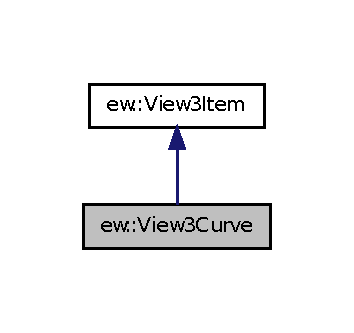
\includegraphics[width=170pt]{classew_1_1View3Curve__inherit__graph}
\end{center}
\end{figure}
\subsubsection*{Public Member Functions}
\begin{DoxyCompactItemize}
\item 
\hyperlink{classew_1_1View3Curve_a7c1a90f7ca7de52c42bff7f5b0cac0d9}{View3Curve} (\hyperlink{classew_1_1View3Widget}{ew::View3Widget} $\ast$\hyperlink{classew_1_1View3Item_a7d765842ec7b9e145cefa37e3dbae658}{view}, int i\_\-type=0)
\item 
void \hyperlink{classew_1_1View3Curve_a3a7ac177b754f5888d1db92af4d18cdb}{set\_\-curve} (const \hyperlink{classew_1_1DataflowCurve3}{ew::DataflowCurve3} $\ast$cur)
\item 
const \hyperlink{classew_1_1DataflowCurve3}{ew::DataflowCurve3} $\ast$ \hyperlink{classew_1_1View3Curve_a70dcbaad96d985a6ab000b9ee0018c6d}{get\_\-curve} () const 
\item 
void \hyperlink{classew_1_1View3Curve_a8b8e42671e07b55cff891847b93a2fe7}{set\_\-color} (const unsigned char $\ast$rgb)
\item 
const unsigned char $\ast$ \hyperlink{classew_1_1View3Curve_a4286dde821d57c24f54dad948f92a827}{get\_\-color} () const 
\end{DoxyCompactItemize}


\subsubsection{Detailed Description}
\hyperlink{classew_1_1View3Curve}{ew::View3Curve} is an \hyperlink{classew_1_1View3Widget}{ew::View3Widget} item to display a \hyperlink{classew_1_1DataflowCurve3}{ew::DataflowCurve3}, a piecewise-\/linear curve.

\hyperlink{classew_1_1View3Curve}{ew::View3Curve} is a class without assignment or comparison. There are private member variables. 

\subsubsection{Constructor \& Destructor Documentation}
\hypertarget{classew_1_1View3Curve_a7c1a90f7ca7de52c42bff7f5b0cac0d9}{
\index{ew::View3Curve@{ew::View3Curve}!View3Curve@{View3Curve}}
\index{View3Curve@{View3Curve}!ew::View3Curve@{ew::View3Curve}}
\paragraph[{View3Curve}]{\setlength{\rightskip}{0pt plus 5cm}ew::View3Curve::View3Curve (
\begin{DoxyParamCaption}
\item[{{\bf ew::View3Widget} $\ast$}]{ view, }
\item[{int}]{ i\_\-type = {\ttfamily 0}}
\end{DoxyParamCaption}
)\hspace{0.3cm}{\ttfamily  \mbox{[}explicit\mbox{]}}}\hfill}
\label{classew_1_1View3Curve_a7c1a90f7ca7de52c42bff7f5b0cac0d9}
This creates an item. 
\begin{DoxyParams}{Parameters}
\item[{\em view}]The view widget the item should belong to. \item[{\em i\_\-type}]The initializer for \hyperlink{classew_1_1View3Item_a7e21fcde8f082ba2409bcb2999a4b7fd}{ew::View3Item::type}. \end{DoxyParams}


\subsubsection{Member Function Documentation}
\hypertarget{classew_1_1View3Curve_a3a7ac177b754f5888d1db92af4d18cdb}{
\index{ew::View3Curve@{ew::View3Curve}!set\_\-curve@{set\_\-curve}}
\index{set\_\-curve@{set\_\-curve}!ew::View3Curve@{ew::View3Curve}}
\paragraph[{set\_\-curve}]{\setlength{\rightskip}{0pt plus 5cm}void ew::View3Curve::set\_\-curve (
\begin{DoxyParamCaption}
\item[{const {\bf ew::DataflowCurve3} $\ast$}]{ cur}
\end{DoxyParamCaption}
)}\hfill}
\label{classew_1_1View3Curve_a3a7ac177b754f5888d1db92af4d18cdb}

\begin{DoxyParams}{Parameters}
\item[{\em cur}]A pointer to the new curve node to display, or 0. \end{DoxyParams}
\hypertarget{classew_1_1View3Curve_a70dcbaad96d985a6ab000b9ee0018c6d}{
\index{ew::View3Curve@{ew::View3Curve}!get\_\-curve@{get\_\-curve}}
\index{get\_\-curve@{get\_\-curve}!ew::View3Curve@{ew::View3Curve}}
\paragraph[{get\_\-curve}]{\setlength{\rightskip}{0pt plus 5cm}const {\bf ew::DataflowCurve3} $\ast$ ew::View3Curve::get\_\-curve (
\begin{DoxyParamCaption}
{}
\end{DoxyParamCaption}
) const\hspace{0.3cm}{\ttfamily  \mbox{[}inline\mbox{]}}}\hfill}
\label{classew_1_1View3Curve_a70dcbaad96d985a6ab000b9ee0018c6d}
\begin{DoxyReturn}{Returns}
A pointer to the current curve node being displayed, or 0. 
\end{DoxyReturn}
\hypertarget{classew_1_1View3Curve_a8b8e42671e07b55cff891847b93a2fe7}{
\index{ew::View3Curve@{ew::View3Curve}!set\_\-color@{set\_\-color}}
\index{set\_\-color@{set\_\-color}!ew::View3Curve@{ew::View3Curve}}
\paragraph[{set\_\-color}]{\setlength{\rightskip}{0pt plus 5cm}void ew::View3Curve::set\_\-color (
\begin{DoxyParamCaption}
\item[{const unsigned char $\ast$}]{ rgb}
\end{DoxyParamCaption}
)}\hfill}
\label{classew_1_1View3Curve_a8b8e42671e07b55cff891847b93a2fe7}

\begin{DoxyParams}{Parameters}
\item[\mbox{\tt[in]} {\em rgb}]This points to an array of size 3 containing the new colour for the curve. \end{DoxyParams}
\hypertarget{classew_1_1View3Curve_a4286dde821d57c24f54dad948f92a827}{
\index{ew::View3Curve@{ew::View3Curve}!get\_\-color@{get\_\-color}}
\index{get\_\-color@{get\_\-color}!ew::View3Curve@{ew::View3Curve}}
\paragraph[{get\_\-color}]{\setlength{\rightskip}{0pt plus 5cm}const unsigned char $\ast$ ew::View3Curve::get\_\-color (
\begin{DoxyParamCaption}
{}
\end{DoxyParamCaption}
) const\hspace{0.3cm}{\ttfamily  \mbox{[}inline\mbox{]}}}\hfill}
\label{classew_1_1View3Curve_a4286dde821d57c24f54dad948f92a827}
\begin{DoxyReturn}{Returns}
A pointer to the current colour for the curve. 
\end{DoxyReturn}

\hypertarget{classew_1_1View3Image}{
\subsection{ew::View3Image Class Reference}
\label{classew_1_1View3Image}\index{ew::View3Image@{ew::View3Image}}
}


Image Item.  




{\ttfamily \#include $<$ew/View3Image.h$>$}



Inheritance diagram for ew::View3Image:
\nopagebreak
\begin{figure}[H]
\begin{center}
\leavevmode
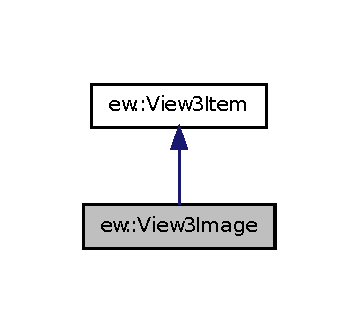
\includegraphics[width=172pt]{classew_1_1View3Image__inherit__graph}
\end{center}
\end{figure}
\subsubsection*{Public Member Functions}
\begin{DoxyCompactItemize}
\item 
\hyperlink{classew_1_1View3Image_ad4dcf5c417e3d26c03e24bd0944f3916}{View3Image} (\hyperlink{classew_1_1View3Widget}{ew::View3Widget} $\ast$\hyperlink{classew_1_1View3Item_a7d765842ec7b9e145cefa37e3dbae658}{view}, int i\_\-type=0)
\item 
void \hyperlink{classew_1_1View3Image_ac419897feabe98bc80ed6f55e5ff574f}{set\_\-image} (const ew::DataflowImage3 $\ast$im)
\item 
const ew::DataflowImage3 $\ast$ \hyperlink{classew_1_1View3Image_a47ffcb6ac24e472adadf4167ab44fc21}{get\_\-image} () const 
\item 
void \hyperlink{classew_1_1View3Image_aae9880444a3b30d5101bc3a864687cef}{set\_\-color} (const unsigned char $\ast$rgb)
\item 
const unsigned char $\ast$ \hyperlink{classew_1_1View3Image_acc36bc0737367a2197e806ed4ac09ece}{get\_\-color} () const 
\end{DoxyCompactItemize}


\subsubsection{Detailed Description}
\hyperlink{classew_1_1View3Image}{ew::View3Image} is an \hyperlink{classew_1_1View3Widget}{ew::View3Widget} item to display a ew::DataflowImage3, a raster image projected onto an array of points.

\hyperlink{classew_1_1View3Image}{ew::View3Image} is a class without assignment or comparison. There are private member variables.

This is barely implemented, and currently just displays a solid rectangle, on a 2x2x1 rectangular array of points.

The default colour is \mbox{[}128, 128, 128\mbox{]}. 

\subsubsection{Constructor \& Destructor Documentation}
\hypertarget{classew_1_1View3Image_ad4dcf5c417e3d26c03e24bd0944f3916}{
\index{ew::View3Image@{ew::View3Image}!View3Image@{View3Image}}
\index{View3Image@{View3Image}!ew::View3Image@{ew::View3Image}}
\paragraph[{View3Image}]{\setlength{\rightskip}{0pt plus 5cm}ew::View3Image::View3Image (
\begin{DoxyParamCaption}
\item[{{\bf ew::View3Widget} $\ast$}]{ view, }
\item[{int}]{ i\_\-type = {\ttfamily 0}}
\end{DoxyParamCaption}
)\hspace{0.3cm}{\ttfamily  \mbox{[}explicit\mbox{]}}}\hfill}
\label{classew_1_1View3Image_ad4dcf5c417e3d26c03e24bd0944f3916}
This creates an item. 
\begin{DoxyParams}{Parameters}
\item[{\em view}]The view widget the item should belong to. \item[{\em i\_\-type}]The initializer for \hyperlink{classew_1_1View3Item_a7e21fcde8f082ba2409bcb2999a4b7fd}{ew::View3Item::type}. \end{DoxyParams}


\subsubsection{Member Function Documentation}
\hypertarget{classew_1_1View3Image_ac419897feabe98bc80ed6f55e5ff574f}{
\index{ew::View3Image@{ew::View3Image}!set\_\-image@{set\_\-image}}
\index{set\_\-image@{set\_\-image}!ew::View3Image@{ew::View3Image}}
\paragraph[{set\_\-image}]{\setlength{\rightskip}{0pt plus 5cm}void ew::View3Image::set\_\-image (
\begin{DoxyParamCaption}
\item[{const ew::DataflowImage3 $\ast$}]{ im}
\end{DoxyParamCaption}
)}\hfill}
\label{classew_1_1View3Image_ac419897feabe98bc80ed6f55e5ff574f}

\begin{DoxyParams}{Parameters}
\item[{\em im}]A pointer to the new image node to display, or 0. \end{DoxyParams}
\hypertarget{classew_1_1View3Image_a47ffcb6ac24e472adadf4167ab44fc21}{
\index{ew::View3Image@{ew::View3Image}!get\_\-image@{get\_\-image}}
\index{get\_\-image@{get\_\-image}!ew::View3Image@{ew::View3Image}}
\paragraph[{get\_\-image}]{\setlength{\rightskip}{0pt plus 5cm}const ew::DataflowImage3 $\ast$ ew::View3Image::get\_\-image (
\begin{DoxyParamCaption}
{}
\end{DoxyParamCaption}
) const\hspace{0.3cm}{\ttfamily  \mbox{[}inline\mbox{]}}}\hfill}
\label{classew_1_1View3Image_a47ffcb6ac24e472adadf4167ab44fc21}
\begin{DoxyReturn}{Returns}
A pointer to the current image node being displayed, or 0. 
\end{DoxyReturn}
\hypertarget{classew_1_1View3Image_aae9880444a3b30d5101bc3a864687cef}{
\index{ew::View3Image@{ew::View3Image}!set\_\-color@{set\_\-color}}
\index{set\_\-color@{set\_\-color}!ew::View3Image@{ew::View3Image}}
\paragraph[{set\_\-color}]{\setlength{\rightskip}{0pt plus 5cm}void ew::View3Image::set\_\-color (
\begin{DoxyParamCaption}
\item[{const unsigned char $\ast$}]{ rgb}
\end{DoxyParamCaption}
)}\hfill}
\label{classew_1_1View3Image_aae9880444a3b30d5101bc3a864687cef}

\begin{DoxyParams}{Parameters}
\item[\mbox{\tt[in]} {\em rgb}]This points to an array of size 3 containing the new colour for the image. \end{DoxyParams}
\hypertarget{classew_1_1View3Image_acc36bc0737367a2197e806ed4ac09ece}{
\index{ew::View3Image@{ew::View3Image}!get\_\-color@{get\_\-color}}
\index{get\_\-color@{get\_\-color}!ew::View3Image@{ew::View3Image}}
\paragraph[{get\_\-color}]{\setlength{\rightskip}{0pt plus 5cm}const unsigned char $\ast$ ew::View3Image::get\_\-color (
\begin{DoxyParamCaption}
{}
\end{DoxyParamCaption}
) const\hspace{0.3cm}{\ttfamily  \mbox{[}inline\mbox{]}}}\hfill}
\label{classew_1_1View3Image_acc36bc0737367a2197e806ed4ac09ece}
\begin{DoxyReturn}{Returns}
A pointer to the current colour for the image. 
\end{DoxyReturn}

\hypertarget{classew_1_1View3Item}{
\subsection{ew::View3Item Class Reference}
\label{classew_1_1View3Item}\index{ew::View3Item@{ew::View3Item}}
}


Item Base Class.  




{\ttfamily \#include $<$ew/View3Item.h$>$}



Inheritance diagram for ew::View3Item:
\nopagebreak
\begin{figure}[H]
\begin{center}
\leavevmode
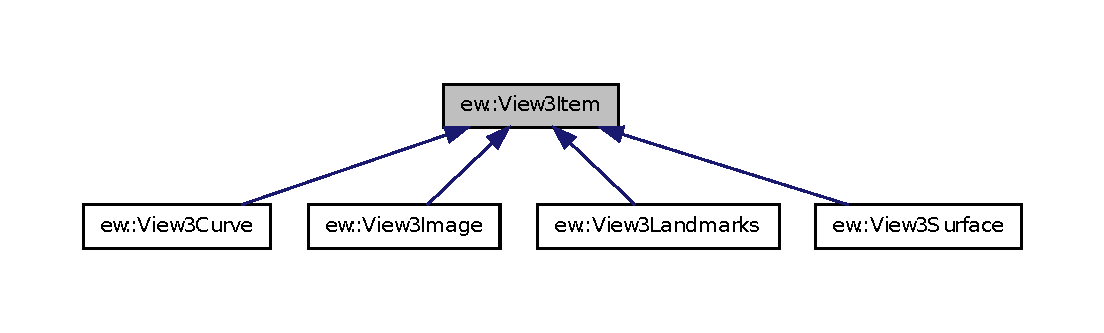
\includegraphics[width=400pt]{classew_1_1View3Item__inherit__graph}
\end{center}
\end{figure}
\subsubsection*{Public Member Functions}
\begin{DoxyCompactItemize}
\item 
bool \hyperlink{classew_1_1View3Item_a73fa1808887496208897b56378d26cd3}{get\_\-state} () const 
\item 
void \hyperlink{classew_1_1View3Item_aebe04d5c9a8a8079d651d7ca179a312c}{set\_\-state} (bool st)
\item 
virtual const \hyperlink{classew_1_1Bbox3}{ew::Bbox3} $\ast$ \hyperlink{classew_1_1View3Item_a9591a8a9c68d627c93e4009c523767c2}{get\_\-bbox} ()=0
\item 
int \hyperlink{classew_1_1View3Item_a25a5d5d4e1fb109b8024966556f35ea2}{get\_\-index} () const 
\item 
void \hyperlink{classew_1_1View3Item_ac111273d2bb3433145be1506125a48de}{destroy} ()
\end{DoxyCompactItemize}
\subsubsection*{Public Attributes}
\begin{DoxyCompactItemize}
\item 
\hyperlink{classew_1_1DataflowNetwork}{ew::DataflowNetwork} $\ast$const \hyperlink{classew_1_1View3Item_af6294268d63629c620cebb3ece227c20}{network}
\item 
\hyperlink{classew_1_1View3Widget}{ew::View3Widget} $\ast$const \hyperlink{classew_1_1View3Item_a7d765842ec7b9e145cefa37e3dbae658}{view}
\item 
const int \hyperlink{classew_1_1View3Item_a7e21fcde8f082ba2409bcb2999a4b7fd}{type}
\end{DoxyCompactItemize}


\subsubsection{Detailed Description}
\hyperlink{classew_1_1View3Item}{ew::View3Item} is the base class for items displayed in ew::View\_\-widget.

\hyperlink{classew_1_1View3Item}{ew::View3Item} is a class without assignment or comparison. There are private member variables.

Items must be created with {\ttfamily new} and then belong to the \hyperlink{classew_1_1View3Widget}{ew::View3Widget}. They must only be deleted indirectly with the \hyperlink{classew_1_1View3Item_ac111273d2bb3433145be1506125a48de}{destroy} method. Remaining items will be automatically deleted when the \hyperlink{classew_1_1View3Widget}{ew::View3Widget} is destroyed. 

\subsubsection{Member Function Documentation}
\hypertarget{classew_1_1View3Item_a73fa1808887496208897b56378d26cd3}{
\index{ew::View3Item@{ew::View3Item}!get\_\-state@{get\_\-state}}
\index{get\_\-state@{get\_\-state}!ew::View3Item@{ew::View3Item}}
\paragraph[{get\_\-state}]{\setlength{\rightskip}{0pt plus 5cm}bool ew::View3Item::get\_\-state (
\begin{DoxyParamCaption}
{}
\end{DoxyParamCaption}
) const\hspace{0.3cm}{\ttfamily  \mbox{[}inline\mbox{]}}}\hfill}
\label{classew_1_1View3Item_a73fa1808887496208897b56378d26cd3}
An item is displayed iff the state is {\ttfamily true}. \begin{DoxyReturn}{Returns}
The current state of the item. 
\end{DoxyReturn}
\hypertarget{classew_1_1View3Item_aebe04d5c9a8a8079d651d7ca179a312c}{
\index{ew::View3Item@{ew::View3Item}!set\_\-state@{set\_\-state}}
\index{set\_\-state@{set\_\-state}!ew::View3Item@{ew::View3Item}}
\paragraph[{set\_\-state}]{\setlength{\rightskip}{0pt plus 5cm}void ew::View3Item::set\_\-state (
\begin{DoxyParamCaption}
\item[{bool}]{ i}
\end{DoxyParamCaption}
)}\hfill}
\label{classew_1_1View3Item_aebe04d5c9a8a8079d651d7ca179a312c}

\begin{DoxyParams}{Parameters}
\item[{\em i}]The new state of the item. \end{DoxyParams}
\hypertarget{classew_1_1View3Item_a9591a8a9c68d627c93e4009c523767c2}{
\index{ew::View3Item@{ew::View3Item}!get\_\-bbox@{get\_\-bbox}}
\index{get\_\-bbox@{get\_\-bbox}!ew::View3Item@{ew::View3Item}}
\paragraph[{get\_\-bbox}]{\setlength{\rightskip}{0pt plus 5cm}const {\bf ew::Bbox3} $\ast$ ew::View3Item::get\_\-bbox (
\begin{DoxyParamCaption}
{}
\end{DoxyParamCaption}
)\hspace{0.3cm}{\ttfamily  \mbox{[}pure virtual\mbox{]}}}\hfill}
\label{classew_1_1View3Item_a9591a8a9c68d627c93e4009c523767c2}
\begin{DoxyReturn}{Returns}
A pointer to a bounding box for the item as currently being displayed. 
\end{DoxyReturn}
\hypertarget{classew_1_1View3Item_a25a5d5d4e1fb109b8024966556f35ea2}{
\index{ew::View3Item@{ew::View3Item}!get\_\-index@{get\_\-index}}
\index{get\_\-index@{get\_\-index}!ew::View3Item@{ew::View3Item}}
\paragraph[{get\_\-index}]{\setlength{\rightskip}{0pt plus 5cm}int ew::View3Item::get\_\-index (
\begin{DoxyParamCaption}
{}
\end{DoxyParamCaption}
) const\hspace{0.3cm}{\ttfamily  \mbox{[}inline\mbox{]}}}\hfill}
\label{classew_1_1View3Item_a25a5d5d4e1fb109b8024966556f35ea2}
\begin{DoxyReturn}{Returns}
The current index of the item in the widget's item list. 
\end{DoxyReturn}
\hypertarget{classew_1_1View3Item_ac111273d2bb3433145be1506125a48de}{
\index{ew::View3Item@{ew::View3Item}!destroy@{destroy}}
\index{destroy@{destroy}!ew::View3Item@{ew::View3Item}}
\paragraph[{destroy}]{\setlength{\rightskip}{0pt plus 5cm}void ew::View3Item::destroy (
\begin{DoxyParamCaption}
{}
\end{DoxyParamCaption}
)\hspace{0.3cm}{\ttfamily  \mbox{[}inline\mbox{]}}}\hfill}
\label{classew_1_1View3Item_ac111273d2bb3433145be1506125a48de}
This removes the item from the widget and destroys it. 

\subsubsection{Member Data Documentation}
\hypertarget{classew_1_1View3Item_af6294268d63629c620cebb3ece227c20}{
\index{ew::View3Item@{ew::View3Item}!network@{network}}
\index{network@{network}!ew::View3Item@{ew::View3Item}}
\paragraph[{network}]{\setlength{\rightskip}{0pt plus 5cm}{\bf ew::DataflowNetwork} $\ast$const {\bf ew::View3Item::network}}\hfill}
\label{classew_1_1View3Item_af6294268d63629c620cebb3ece227c20}
This points to the \hyperlink{classew_1_1DataflowNetwork}{ew::DataflowNetwork} that the \hyperlink{classew_1_1View3Item_a7d765842ec7b9e145cefa37e3dbae658}{view} was created with. \hypertarget{classew_1_1View3Item_a7d765842ec7b9e145cefa37e3dbae658}{
\index{ew::View3Item@{ew::View3Item}!view@{view}}
\index{view@{view}!ew::View3Item@{ew::View3Item}}
\paragraph[{view}]{\setlength{\rightskip}{0pt plus 5cm}{\bf ew::View3Widget} $\ast$const {\bf ew::View3Item::view}}\hfill}
\label{classew_1_1View3Item_a7d765842ec7b9e145cefa37e3dbae658}
This points to the \hyperlink{classew_1_1View3Widget}{ew::View3Widget} the this \hyperlink{classew_1_1View3Item}{ew::View3Item} was created with. \hypertarget{classew_1_1View3Item_a7e21fcde8f082ba2409bcb2999a4b7fd}{
\index{ew::View3Item@{ew::View3Item}!type@{type}}
\index{type@{type}!ew::View3Item@{ew::View3Item}}
\paragraph[{type}]{\setlength{\rightskip}{0pt plus 5cm}const int {\bf ew::View3Item::type}}\hfill}
\label{classew_1_1View3Item_a7e21fcde8f082ba2409bcb2999a4b7fd}
This is an arbitrary value supplied in the constructor. It is client data, not touched by \hyperlink{classew_1_1View3Item}{ew::View3Item} or \hyperlink{classew_1_1View3Widget}{ew::View3Widget}. 
\hypertarget{classew_1_1View3Landmarks}{
\subsection{ew::View3Landmarks Class Reference}
\label{classew_1_1View3Landmarks}\index{ew::View3Landmarks@{ew::View3Landmarks}}
}


Landmarks Item.  




{\ttfamily \#include $<$ew/View3Landmarks.h$>$}



Inheritance diagram for ew::View3Landmarks:
\nopagebreak
\begin{figure}[H]
\begin{center}
\leavevmode
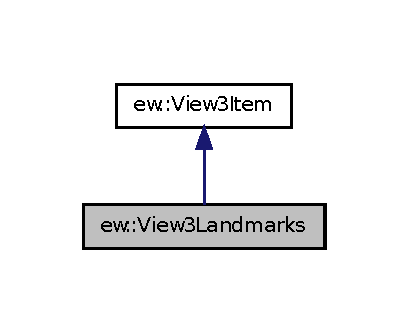
\includegraphics[width=196pt]{classew_1_1View3Landmarks__inherit__graph}
\end{center}
\end{figure}
\subsubsection*{Public Types}
\begin{DoxyCompactItemize}
\item 
enum \hyperlink{classew_1_1View3Landmarks_a1568c52b9714e8042cfdc7a1835413c4}{symbol\_\-t} \{ \hyperlink{classew_1_1View3Landmarks_a1568c52b9714e8042cfdc7a1835413c4a0844a595f6fe10dff5493050cbc31a2c}{SYMBOL\_\-CROSS}, 
\hyperlink{classew_1_1View3Landmarks_a1568c52b9714e8042cfdc7a1835413c4a1f2350f74b86929d03442b7c7fccbf88}{SYMBOL\_\-CIRCLE}, 
\hyperlink{classew_1_1View3Landmarks_a1568c52b9714e8042cfdc7a1835413c4ae45cc6c7d43c3c5924d55612b3c193e8}{SYMBOL\_\-DOT}
 \}
\end{DoxyCompactItemize}
\subsubsection*{Public Member Functions}
\begin{DoxyCompactItemize}
\item 
\hyperlink{classew_1_1View3Landmarks_ac2b94a222f9c767f376386648163e21e}{View3Landmarks} (\hyperlink{classew_1_1View3Widget}{ew::View3Widget} $\ast$\hyperlink{classew_1_1View3Item_a7d765842ec7b9e145cefa37e3dbae658}{view}, int i\_\-type=0)
\item 
void \hyperlink{classew_1_1View3Landmarks_a28b6615870a90c8179023827796bbc45}{set\_\-form} (const \hyperlink{classew_1_1DataflowForm3}{ew::DataflowForm3} $\ast$frm)
\item 
const \hyperlink{classew_1_1DataflowForm3}{ew::DataflowForm3} $\ast$ \hyperlink{classew_1_1View3Landmarks_ad41875336f92f693fa215137305a09ed}{get\_\-form} () const 
\item 
void \hyperlink{classew_1_1View3Landmarks_a72cad881f909b1105ef46ab53f9b2801}{set\_\-color} (const unsigned char $\ast$rgb)
\item 
const unsigned char $\ast$ \hyperlink{classew_1_1View3Landmarks_aff46a81fe7ec6bd3895dbe9ea6630230}{get\_\-color} () const 
\item 
void \hyperlink{classew_1_1View3Landmarks_a5215584e89b18fca5f9b53e6943d6ffe}{set\_\-highlight} (int ps, int i)
\item 
int \hyperlink{classew_1_1View3Landmarks_ad39299ed05ded5379e4f8749e8eaa2a3}{get\_\-highlight\_\-ps} () const 
\item 
int \hyperlink{classew_1_1View3Landmarks_a2c4b9e20c783af8f296868b04ad4711a}{get\_\-highlight\_\-i} () const 
\item 
void \hyperlink{classew_1_1View3Landmarks_ae6dfece42f463c68bfc76f3782fd5006}{set\_\-symbol} (int sym)
\item 
int \hyperlink{classew_1_1View3Landmarks_a6144e736708e87f05fe35fccc1963626}{get\_\-symbol} () const 
\end{DoxyCompactItemize}
\subsubsection*{Static Public Attributes}
\begin{DoxyCompactItemize}
\item 
static const int \hyperlink{classew_1_1View3Landmarks_a2aac16ae4a3bc617df69e9a881309011}{N\_\-SYMBOLS} = 3
\item 
static const char $\ast$const \hyperlink{classew_1_1View3Landmarks_acf1fcc64c77ecabaee9ad645a46a707c}{symbol\_\-names} \mbox{[}$\,$\mbox{]}
\end{DoxyCompactItemize}


\subsubsection{Detailed Description}
\hyperlink{classew_1_1View3Landmarks}{ew::View3Landmarks} is an \hyperlink{classew_1_1View3Widget}{ew::View3Widget} item to display the landmarks in a \hyperlink{classew_1_1DataflowForm3}{ew::DataflowForm3}.

\hyperlink{classew_1_1View3Landmarks}{ew::View3Landmarks} is a class without assignment or comparison. There are private member variables. 

\subsubsection{Member Enumeration Documentation}
\hypertarget{classew_1_1View3Landmarks_a1568c52b9714e8042cfdc7a1835413c4}{
\index{ew::View3Landmarks@{ew::View3Landmarks}!symbol\_\-t@{symbol\_\-t}}
\index{symbol\_\-t@{symbol\_\-t}!ew::View3Landmarks@{ew::View3Landmarks}}
\paragraph[{symbol\_\-t}]{\setlength{\rightskip}{0pt plus 5cm}enum {\bf ew::View3Landmarks::symbol\_\-t}}\hfill}
\label{classew_1_1View3Landmarks_a1568c52b9714e8042cfdc7a1835413c4}
These are the possible values for \hyperlink{classew_1_1View3Landmarks_ae6dfece42f463c68bfc76f3782fd5006}{set\_\-symbol} and \hyperlink{classew_1_1View3Landmarks_a6144e736708e87f05fe35fccc1963626}{get\_\-symbol}. The first, with value zero, is \hyperlink{classew_1_1View3Landmarks_a1568c52b9714e8042cfdc7a1835413c4a0844a595f6fe10dff5493050cbc31a2c}{SYMBOL\_\-CROSS}. \begin{Desc}
\item[Enumerator: ]\par
\begin{description}
\index{SYMBOL\_\-CROSS@{SYMBOL\_\-CROSS}!ew::View3Landmarks@{ew::View3Landmarks}}\index{ew::View3Landmarks@{ew::View3Landmarks}!SYMBOL\_\-CROSS@{SYMBOL\_\-CROSS}}\item[{\em 
\hypertarget{classew_1_1View3Landmarks_a1568c52b9714e8042cfdc7a1835413c4a0844a595f6fe10dff5493050cbc31a2c}{
SYMBOL\_\-CROSS}
\label{classew_1_1View3Landmarks_a1568c52b9714e8042cfdc7a1835413c4a0844a595f6fe10dff5493050cbc31a2c}
}]A cross symbol. \index{SYMBOL\_\-CIRCLE@{SYMBOL\_\-CIRCLE}!ew::View3Landmarks@{ew::View3Landmarks}}\index{ew::View3Landmarks@{ew::View3Landmarks}!SYMBOL\_\-CIRCLE@{SYMBOL\_\-CIRCLE}}\item[{\em 
\hypertarget{classew_1_1View3Landmarks_a1568c52b9714e8042cfdc7a1835413c4a1f2350f74b86929d03442b7c7fccbf88}{
SYMBOL\_\-CIRCLE}
\label{classew_1_1View3Landmarks_a1568c52b9714e8042cfdc7a1835413c4a1f2350f74b86929d03442b7c7fccbf88}
}]A circle symbol. \index{SYMBOL\_\-DOT@{SYMBOL\_\-DOT}!ew::View3Landmarks@{ew::View3Landmarks}}\index{ew::View3Landmarks@{ew::View3Landmarks}!SYMBOL\_\-DOT@{SYMBOL\_\-DOT}}\item[{\em 
\hypertarget{classew_1_1View3Landmarks_a1568c52b9714e8042cfdc7a1835413c4ae45cc6c7d43c3c5924d55612b3c193e8}{
SYMBOL\_\-DOT}
\label{classew_1_1View3Landmarks_a1568c52b9714e8042cfdc7a1835413c4ae45cc6c7d43c3c5924d55612b3c193e8}
}]A dot symbol. \end{description}
\end{Desc}



\subsubsection{Constructor \& Destructor Documentation}
\hypertarget{classew_1_1View3Landmarks_ac2b94a222f9c767f376386648163e21e}{
\index{ew::View3Landmarks@{ew::View3Landmarks}!View3Landmarks@{View3Landmarks}}
\index{View3Landmarks@{View3Landmarks}!ew::View3Landmarks@{ew::View3Landmarks}}
\paragraph[{View3Landmarks}]{\setlength{\rightskip}{0pt plus 5cm}ew::View3Landmarks::View3Landmarks (
\begin{DoxyParamCaption}
\item[{{\bf ew::View3Widget} $\ast$}]{ i\_\-view, }
\item[{int}]{ i\_\-type = {\ttfamily 0}}
\end{DoxyParamCaption}
)\hspace{0.3cm}{\ttfamily  \mbox{[}explicit\mbox{]}}}\hfill}
\label{classew_1_1View3Landmarks_ac2b94a222f9c767f376386648163e21e}
This creates an item. 
\begin{DoxyParams}{Parameters}
\item[{\em view\_\-i}]The view widget the item should belong to. \item[{\em type\_\-i}]The initializer for \hyperlink{classew_1_1View3Item_a7e21fcde8f082ba2409bcb2999a4b7fd}{ew::View3Item::type}. \end{DoxyParams}


\subsubsection{Member Function Documentation}
\hypertarget{classew_1_1View3Landmarks_a28b6615870a90c8179023827796bbc45}{
\index{ew::View3Landmarks@{ew::View3Landmarks}!set\_\-form@{set\_\-form}}
\index{set\_\-form@{set\_\-form}!ew::View3Landmarks@{ew::View3Landmarks}}
\paragraph[{set\_\-form}]{\setlength{\rightskip}{0pt plus 5cm}void ew::View3Landmarks::set\_\-form (
\begin{DoxyParamCaption}
\item[{const {\bf ew::DataflowForm3} $\ast$}]{ frm}
\end{DoxyParamCaption}
)}\hfill}
\label{classew_1_1View3Landmarks_a28b6615870a90c8179023827796bbc45}

\begin{DoxyParams}{Parameters}
\item[{\em frm}]A pointer to the new form node to display, or 0. \end{DoxyParams}
\hypertarget{classew_1_1View3Landmarks_ad41875336f92f693fa215137305a09ed}{
\index{ew::View3Landmarks@{ew::View3Landmarks}!get\_\-form@{get\_\-form}}
\index{get\_\-form@{get\_\-form}!ew::View3Landmarks@{ew::View3Landmarks}}
\paragraph[{get\_\-form}]{\setlength{\rightskip}{0pt plus 5cm}const {\bf ew::DataflowForm3} $\ast$ ew::View3Landmarks::get\_\-form (
\begin{DoxyParamCaption}
{}
\end{DoxyParamCaption}
) const\hspace{0.3cm}{\ttfamily  \mbox{[}inline\mbox{]}}}\hfill}
\label{classew_1_1View3Landmarks_ad41875336f92f693fa215137305a09ed}
\begin{DoxyReturn}{Returns}
A pointer to the current form node being displayed, or 0. 
\end{DoxyReturn}
\hypertarget{classew_1_1View3Landmarks_a72cad881f909b1105ef46ab53f9b2801}{
\index{ew::View3Landmarks@{ew::View3Landmarks}!set\_\-color@{set\_\-color}}
\index{set\_\-color@{set\_\-color}!ew::View3Landmarks@{ew::View3Landmarks}}
\paragraph[{set\_\-color}]{\setlength{\rightskip}{0pt plus 5cm}void ew::View3Landmarks::set\_\-color (
\begin{DoxyParamCaption}
\item[{const unsigned char $\ast$}]{ rgb}
\end{DoxyParamCaption}
)}\hfill}
\label{classew_1_1View3Landmarks_a72cad881f909b1105ef46ab53f9b2801}

\begin{DoxyParams}{Parameters}
\item[\mbox{\tt[in]} {\em rgb}]This points to an array of size 3 containing the new colour for the landmark symbols. \end{DoxyParams}
\hypertarget{classew_1_1View3Landmarks_aff46a81fe7ec6bd3895dbe9ea6630230}{
\index{ew::View3Landmarks@{ew::View3Landmarks}!get\_\-color@{get\_\-color}}
\index{get\_\-color@{get\_\-color}!ew::View3Landmarks@{ew::View3Landmarks}}
\paragraph[{get\_\-color}]{\setlength{\rightskip}{0pt plus 5cm}const unsigned char $\ast$ ew::View3Landmarks::get\_\-color (
\begin{DoxyParamCaption}
{}
\end{DoxyParamCaption}
) const\hspace{0.3cm}{\ttfamily  \mbox{[}inline\mbox{]}}}\hfill}
\label{classew_1_1View3Landmarks_aff46a81fe7ec6bd3895dbe9ea6630230}
\begin{DoxyReturn}{Returns}
A pointer to the current colour for the landmark symbols. 
\end{DoxyReturn}
\hypertarget{classew_1_1View3Landmarks_a5215584e89b18fca5f9b53e6943d6ffe}{
\index{ew::View3Landmarks@{ew::View3Landmarks}!set\_\-highlight@{set\_\-highlight}}
\index{set\_\-highlight@{set\_\-highlight}!ew::View3Landmarks@{ew::View3Landmarks}}
\paragraph[{set\_\-highlight}]{\setlength{\rightskip}{0pt plus 5cm}void ew::View3Landmarks::set\_\-highlight (
\begin{DoxyParamCaption}
\item[{int}]{ ps, }
\item[{int}]{ i}
\end{DoxyParamCaption}
)}\hfill}
\label{classew_1_1View3Landmarks_a5215584e89b18fca5f9b53e6943d6ffe}

\begin{DoxyParams}{Parameters}
\item[{\em ps}]The pointset of the landmark to highlight. \item[{\em i}]The index of the landmark within the pointset of the landmark to highlight. \end{DoxyParams}
\hypertarget{classew_1_1View3Landmarks_ad39299ed05ded5379e4f8749e8eaa2a3}{
\index{ew::View3Landmarks@{ew::View3Landmarks}!get\_\-highlight\_\-ps@{get\_\-highlight\_\-ps}}
\index{get\_\-highlight\_\-ps@{get\_\-highlight\_\-ps}!ew::View3Landmarks@{ew::View3Landmarks}}
\paragraph[{get\_\-highlight\_\-ps}]{\setlength{\rightskip}{0pt plus 5cm}int ew::View3Landmarks::get\_\-highlight\_\-ps (
\begin{DoxyParamCaption}
{}
\end{DoxyParamCaption}
) const\hspace{0.3cm}{\ttfamily  \mbox{[}inline\mbox{]}}}\hfill}
\label{classew_1_1View3Landmarks_ad39299ed05ded5379e4f8749e8eaa2a3}
\begin{DoxyReturn}{Returns}
The currently highlighted pointset index, or -\/1. 
\end{DoxyReturn}
\hypertarget{classew_1_1View3Landmarks_a2c4b9e20c783af8f296868b04ad4711a}{
\index{ew::View3Landmarks@{ew::View3Landmarks}!get\_\-highlight\_\-i@{get\_\-highlight\_\-i}}
\index{get\_\-highlight\_\-i@{get\_\-highlight\_\-i}!ew::View3Landmarks@{ew::View3Landmarks}}
\paragraph[{get\_\-highlight\_\-i}]{\setlength{\rightskip}{0pt plus 5cm}int ew::View3Landmarks::get\_\-highlight\_\-i (
\begin{DoxyParamCaption}
{}
\end{DoxyParamCaption}
) const\hspace{0.3cm}{\ttfamily  \mbox{[}inline\mbox{]}}}\hfill}
\label{classew_1_1View3Landmarks_a2c4b9e20c783af8f296868b04ad4711a}
\begin{DoxyReturn}{Returns}
The currently highlighted landmark index within the pointset, or -\/1. 
\end{DoxyReturn}
\hypertarget{classew_1_1View3Landmarks_ae6dfece42f463c68bfc76f3782fd5006}{
\index{ew::View3Landmarks@{ew::View3Landmarks}!set\_\-symbol@{set\_\-symbol}}
\index{set\_\-symbol@{set\_\-symbol}!ew::View3Landmarks@{ew::View3Landmarks}}
\paragraph[{set\_\-symbol}]{\setlength{\rightskip}{0pt plus 5cm}void ew::View3Landmarks::set\_\-symbol (
\begin{DoxyParamCaption}
\item[{int}]{ sym}
\end{DoxyParamCaption}
)}\hfill}
\label{classew_1_1View3Landmarks_ae6dfece42f463c68bfc76f3782fd5006}

\begin{DoxyParams}{Parameters}
\item[{\em sym}]The new landmark symbol. \end{DoxyParams}
\hypertarget{classew_1_1View3Landmarks_a6144e736708e87f05fe35fccc1963626}{
\index{ew::View3Landmarks@{ew::View3Landmarks}!get\_\-symbol@{get\_\-symbol}}
\index{get\_\-symbol@{get\_\-symbol}!ew::View3Landmarks@{ew::View3Landmarks}}
\paragraph[{get\_\-symbol}]{\setlength{\rightskip}{0pt plus 5cm}int ew::View3Landmarks::get\_\-symbol (
\begin{DoxyParamCaption}
{}
\end{DoxyParamCaption}
) const\hspace{0.3cm}{\ttfamily  \mbox{[}inline\mbox{]}}}\hfill}
\label{classew_1_1View3Landmarks_a6144e736708e87f05fe35fccc1963626}
\begin{DoxyReturn}{Returns}
The current landmark symbol. 
\end{DoxyReturn}


\subsubsection{Member Data Documentation}
\hypertarget{classew_1_1View3Landmarks_a2aac16ae4a3bc617df69e9a881309011}{
\index{ew::View3Landmarks@{ew::View3Landmarks}!N\_\-SYMBOLS@{N\_\-SYMBOLS}}
\index{N\_\-SYMBOLS@{N\_\-SYMBOLS}!ew::View3Landmarks@{ew::View3Landmarks}}
\paragraph[{N\_\-SYMBOLS}]{\setlength{\rightskip}{0pt plus 5cm}const int {\bf ew::View3Landmarks::N\_\-SYMBOLS} = 3\hspace{0.3cm}{\ttfamily  \mbox{[}static\mbox{]}}}\hfill}
\label{classew_1_1View3Landmarks_a2aac16ae4a3bc617df69e9a881309011}
They number of possible \hyperlink{classew_1_1View3Landmarks_a1568c52b9714e8042cfdc7a1835413c4}{symbol\_\-t} values. \hypertarget{classew_1_1View3Landmarks_acf1fcc64c77ecabaee9ad645a46a707c}{
\index{ew::View3Landmarks@{ew::View3Landmarks}!symbol\_\-names@{symbol\_\-names}}
\index{symbol\_\-names@{symbol\_\-names}!ew::View3Landmarks@{ew::View3Landmarks}}
\paragraph[{symbol\_\-names}]{\setlength{\rightskip}{0pt plus 5cm}const char $\ast$const {\bf ew::View3Landmarks::symbol\_\-names}\hspace{0.3cm}{\ttfamily  \mbox{[}static\mbox{]}}}\hfill}
\label{classew_1_1View3Landmarks_acf1fcc64c77ecabaee9ad645a46a707c}
{\bfseries Initial value:}
\begin{DoxyCode}
 {
  "cross",
  "circle",
  "dot",
  0
}
\end{DoxyCode}
The names of the \hyperlink{classew_1_1View3Landmarks_a1568c52b9714e8042cfdc7a1835413c4}{symbol\_\-t} choices. 
\hypertarget{classew_1_1View3Surface}{
\subsection{ew::View3Surface Class Reference}
\label{classew_1_1View3Surface}\index{ew::View3Surface@{ew::View3Surface}}
}


Surface Item.  




{\ttfamily \#include $<$ew/View3Surface.h$>$}



Inheritance diagram for ew::View3Surface:
\nopagebreak
\begin{figure}[H]
\begin{center}
\leavevmode
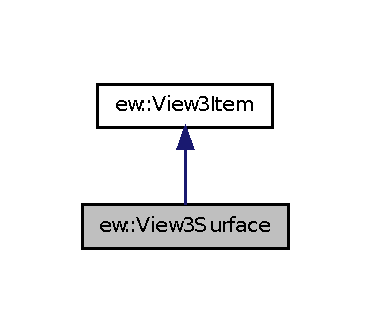
\includegraphics[width=178pt]{classew_1_1View3Surface__inherit__graph}
\end{center}
\end{figure}
\subsubsection*{Public Member Functions}
\begin{DoxyCompactItemize}
\item 
\hyperlink{classew_1_1View3Surface_a93b345f7747e3d073eaff2078c4cb920}{View3Surface} (\hyperlink{classew_1_1View3Widget}{ew::View3Widget} $\ast$\hyperlink{classew_1_1View3Item_a7d765842ec7b9e145cefa37e3dbae658}{view}, int i\_\-type=0)
\item 
void \hyperlink{classew_1_1View3Surface_a58f47bb37d9757ab55c40d83b67f8a68}{set\_\-surface} (const \hyperlink{classew_1_1DataflowSurface3}{ew::DataflowSurface3} $\ast$sur)
\item 
const \hyperlink{classew_1_1DataflowSurface3}{ew::DataflowSurface3} $\ast$ \hyperlink{classew_1_1View3Surface_a8821eb2ee5bd46dbd36cb18a084fa77b}{get\_\-surface} () const 
\item 
void \hyperlink{classew_1_1View3Surface_adae42c158ed8296b2953017f785f70df}{set\_\-front\_\-color} (const unsigned char $\ast$rgb)
\item 
const unsigned char $\ast$ \hyperlink{classew_1_1View3Surface_ab3c6316ff0e5489d663800aefd27e28d}{get\_\-front\_\-color} () const 
\item 
void \hyperlink{classew_1_1View3Surface_a604dbde29cdbac1eddbb474813d8ce49}{set\_\-back\_\-color} (const unsigned char $\ast$rgb)
\item 
const unsigned char $\ast$ \hyperlink{classew_1_1View3Surface_aa35528b961596719233e5c0f41cd9efb}{get\_\-back\_\-color} () const 
\end{DoxyCompactItemize}


\subsubsection{Detailed Description}
\hyperlink{classew_1_1View3Surface}{ew::View3Surface} is an \hyperlink{classew_1_1View3Widget}{ew::View3Widget} item to display a \hyperlink{classew_1_1DataflowSurface3}{ew::DataflowSurface3}, a triangulated surface.

\hyperlink{classew_1_1View3Surface}{ew::View3Surface} is a class without assignment or comparison. There are private member variables. 

\subsubsection{Constructor \& Destructor Documentation}
\hypertarget{classew_1_1View3Surface_a93b345f7747e3d073eaff2078c4cb920}{
\index{ew::View3Surface@{ew::View3Surface}!View3Surface@{View3Surface}}
\index{View3Surface@{View3Surface}!ew::View3Surface@{ew::View3Surface}}
\paragraph[{View3Surface}]{\setlength{\rightskip}{0pt plus 5cm}ew::View3Surface::View3Surface (
\begin{DoxyParamCaption}
\item[{{\bf ew::View3Widget} $\ast$}]{ v, }
\item[{int}]{ i\_\-type = {\ttfamily 0}}
\end{DoxyParamCaption}
)\hspace{0.3cm}{\ttfamily  \mbox{[}explicit\mbox{]}}}\hfill}
\label{classew_1_1View3Surface_a93b345f7747e3d073eaff2078c4cb920}
This creates an item. 
\begin{DoxyParams}{Parameters}
\item[{\em v}]The view widget the item should belong to. \item[{\em type\_\-i}]The initializer for \hyperlink{classew_1_1View3Item_a7e21fcde8f082ba2409bcb2999a4b7fd}{ew::View3Item::type}. \end{DoxyParams}


\subsubsection{Member Function Documentation}
\hypertarget{classew_1_1View3Surface_a58f47bb37d9757ab55c40d83b67f8a68}{
\index{ew::View3Surface@{ew::View3Surface}!set\_\-surface@{set\_\-surface}}
\index{set\_\-surface@{set\_\-surface}!ew::View3Surface@{ew::View3Surface}}
\paragraph[{set\_\-surface}]{\setlength{\rightskip}{0pt plus 5cm}void ew::View3Surface::set\_\-surface (
\begin{DoxyParamCaption}
\item[{const {\bf ew::DataflowSurface3} $\ast$}]{ s}
\end{DoxyParamCaption}
)}\hfill}
\label{classew_1_1View3Surface_a58f47bb37d9757ab55c40d83b67f8a68}

\begin{DoxyParams}{Parameters}
\item[{\em s}]A pointer to the new surface node to display, or 0. \end{DoxyParams}
\hypertarget{classew_1_1View3Surface_a8821eb2ee5bd46dbd36cb18a084fa77b}{
\index{ew::View3Surface@{ew::View3Surface}!get\_\-surface@{get\_\-surface}}
\index{get\_\-surface@{get\_\-surface}!ew::View3Surface@{ew::View3Surface}}
\paragraph[{get\_\-surface}]{\setlength{\rightskip}{0pt plus 5cm}const {\bf ew::DataflowSurface3} $\ast$ ew::View3Surface::get\_\-surface (
\begin{DoxyParamCaption}
{}
\end{DoxyParamCaption}
) const\hspace{0.3cm}{\ttfamily  \mbox{[}inline\mbox{]}}}\hfill}
\label{classew_1_1View3Surface_a8821eb2ee5bd46dbd36cb18a084fa77b}
\begin{DoxyReturn}{Returns}
A pointer to the current surface node being displayed, or 0. 
\end{DoxyReturn}
\hypertarget{classew_1_1View3Surface_adae42c158ed8296b2953017f785f70df}{
\index{ew::View3Surface@{ew::View3Surface}!set\_\-front\_\-color@{set\_\-front\_\-color}}
\index{set\_\-front\_\-color@{set\_\-front\_\-color}!ew::View3Surface@{ew::View3Surface}}
\paragraph[{set\_\-front\_\-color}]{\setlength{\rightskip}{0pt plus 5cm}void ew::View3Surface::set\_\-front\_\-color (
\begin{DoxyParamCaption}
\item[{const unsigned char $\ast$}]{ rgb}
\end{DoxyParamCaption}
)}\hfill}
\label{classew_1_1View3Surface_adae42c158ed8296b2953017f785f70df}

\begin{DoxyParams}{Parameters}
\item[\mbox{\tt[in]} {\em rgb}]This points to an array of size 3 containing the new colour for the front of the surface. \end{DoxyParams}
\hypertarget{classew_1_1View3Surface_ab3c6316ff0e5489d663800aefd27e28d}{
\index{ew::View3Surface@{ew::View3Surface}!get\_\-front\_\-color@{get\_\-front\_\-color}}
\index{get\_\-front\_\-color@{get\_\-front\_\-color}!ew::View3Surface@{ew::View3Surface}}
\paragraph[{get\_\-front\_\-color}]{\setlength{\rightskip}{0pt plus 5cm}const unsigned char $\ast$ ew::View3Surface::get\_\-front\_\-color (
\begin{DoxyParamCaption}
{}
\end{DoxyParamCaption}
) const\hspace{0.3cm}{\ttfamily  \mbox{[}inline\mbox{]}}}\hfill}
\label{classew_1_1View3Surface_ab3c6316ff0e5489d663800aefd27e28d}
\begin{DoxyReturn}{Returns}
A pointer to the current colour for the front of the surface. 
\end{DoxyReturn}
\hypertarget{classew_1_1View3Surface_a604dbde29cdbac1eddbb474813d8ce49}{
\index{ew::View3Surface@{ew::View3Surface}!set\_\-back\_\-color@{set\_\-back\_\-color}}
\index{set\_\-back\_\-color@{set\_\-back\_\-color}!ew::View3Surface@{ew::View3Surface}}
\paragraph[{set\_\-back\_\-color}]{\setlength{\rightskip}{0pt plus 5cm}void ew::View3Surface::set\_\-back\_\-color (
\begin{DoxyParamCaption}
\item[{const unsigned char $\ast$}]{ rgb}
\end{DoxyParamCaption}
)}\hfill}
\label{classew_1_1View3Surface_a604dbde29cdbac1eddbb474813d8ce49}

\begin{DoxyParams}{Parameters}
\item[\mbox{\tt[in]} {\em rgb}]This points to an array of size 3 containing the new colour for the back of the surface. \end{DoxyParams}
\hypertarget{classew_1_1View3Surface_aa35528b961596719233e5c0f41cd9efb}{
\index{ew::View3Surface@{ew::View3Surface}!get\_\-back\_\-color@{get\_\-back\_\-color}}
\index{get\_\-back\_\-color@{get\_\-back\_\-color}!ew::View3Surface@{ew::View3Surface}}
\paragraph[{get\_\-back\_\-color}]{\setlength{\rightskip}{0pt plus 5cm}const unsigned char $\ast$ ew::View3Surface::get\_\-back\_\-color (
\begin{DoxyParamCaption}
{}
\end{DoxyParamCaption}
) const\hspace{0.3cm}{\ttfamily  \mbox{[}inline\mbox{]}}}\hfill}
\label{classew_1_1View3Surface_aa35528b961596719233e5c0f41cd9efb}
\begin{DoxyReturn}{Returns}
A pointer to the current colour for the back of the surface. 
\end{DoxyReturn}

\hypertarget{classew_1_1View3Widget}{
\subsection{ew::View3Widget Class Reference}
\label{classew_1_1View3Widget}\index{ew::View3Widget@{ew::View3Widget}}
}


3D viewing widget  




{\ttfamily \#include $<$ew/View3Widget.h$>$}



Inheritance diagram for ew::View3Widget:
\nopagebreak
\begin{figure}[H]
\begin{center}
\leavevmode
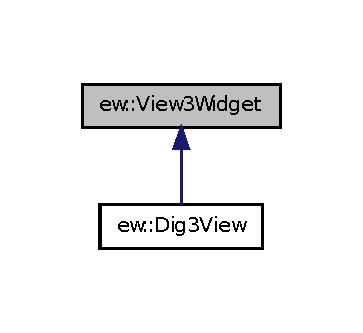
\includegraphics[width=174pt]{classew_1_1View3Widget__inherit__graph}
\end{center}
\end{figure}
\subsubsection*{Public Member Functions}
\begin{DoxyCompactItemize}
\item 
\hyperlink{classew_1_1View3Widget_a02c6cc328ca2134102edb1f88fea3ad2}{View3Widget} (\hyperlink{classew_1_1DataflowNetwork}{ew::DataflowNetwork} $\ast$i\_\-network)
\item 
virtual \hyperlink{classew_1_1View3Widget_a83833294148eeb392dc5cbadde2e51f0}{$\sim$View3Widget} ()
\item 
void \hyperlink{classew_1_1View3Widget_afc90fcfe34fb1cdbad10f437e75673a7}{reset} ()
\item 
void \hyperlink{classew_1_1View3Widget_a79673466aa3cb43d392448544853b5e1}{set\_\-clip\_\-ratio} (double cr)
\item 
double \hyperlink{classew_1_1View3Widget_a1b2c3e56f12c09a56e55a1e4f6a5820c}{get\_\-clip\_\-ratio} () const 
\item 
void \hyperlink{classew_1_1View3Widget_aca4dfffefdc6bf300e6f26ef76bb1913}{set\_\-view\_\-mapping} (const \hyperlink{classew_1_1Transform3}{ew::Transform3} $\ast$tr)
\item 
void \hyperlink{classew_1_1View3Widget_a90e7e1db3ccb509999f68e3aa23d27f5}{view\_\-post\_\-compose} (const \hyperlink{classew_1_1Transform3}{ew::Transform3} $\ast$tr)
\item 
const \hyperlink{classew_1_1Transform3}{ew::Transform3} $\ast$ \hyperlink{classew_1_1View3Widget_ac7d97d4e5fe84c860dc9aef539e034f5}{get\_\-view\_\-mapping} () const 
\item 
void \hyperlink{classew_1_1View3Widget_aa7a23dd2ef40661ec6ba2216807983fb}{get\_\-bbox} (\hyperlink{classew_1_1Bbox3}{ew::Bbox3} $\ast$b) const 
\item 
void \hyperlink{classew_1_1View3Widget_aca913dd88a37bd4d614c9f21eef5f3f6}{get\_\-pointer\_\-location} (double $\ast$loc, double x, double y, double z=0.0) const 
\item 
void \hyperlink{classew_1_1View3Widget_aec2e2c037ab83b6ff89f940b0e5a053a}{get\_\-center\_\-location} (double $\ast$loc) const 
\item 
void \hyperlink{classew_1_1View3Widget_a2ee54b43d51423eb3d7eb15aed4d69f4}{get\_\-pointer\_\-translate\_\-tr} (\hyperlink{classew_1_1Transform3}{ew::Transform3} $\ast$tr, double x, double y, double z) const 
\item 
void \hyperlink{classew_1_1View3Widget_ac29f5fc8232cf56db50a06493d31d1ff}{get\_\-pointer\_\-roll\_\-tr} (\hyperlink{classew_1_1Transform3}{ew::Transform3} $\ast$tr, double x, double y) const 
\item 
void \hyperlink{classew_1_1View3Widget_aed81f4b06017dcd6f7095ffbe336cc36}{get\_\-pointer\_\-twist\_\-tr} (\hyperlink{classew_1_1Transform3}{ew::Transform3} $\ast$tr, double x0, double y0, double x1, double y1, double acc) const 
\item 
void \hyperlink{classew_1_1View3Widget_aad8067affea3157ffdf0a1244d5b45a0}{get\_\-pointer\_\-scale\_\-tr} (\hyperlink{classew_1_1Transform3}{ew::Transform3} $\ast$tr, double x0, double y0, double x1, double y1, double acc) const 
\item 
void \hyperlink{classew_1_1View3Widget_addd0136b3a10935e7debc2ed8ce63f6a}{get\_\-jump\_\-tr} (\hyperlink{classew_1_1Transform3}{ew::Transform3} $\ast$tr, const double $\ast$loc, bool do\_\-z) const 
\item 
bool \hyperlink{classew_1_1View3Widget_a47413c17524f0468f3a00e267613a40e}{get\_\-bbox\_\-tr} (\hyperlink{classew_1_1Transform3}{ew::Transform3} $\ast$tr, const \hyperlink{classew_1_1Bbox3}{ew::Bbox3} $\ast$bbox, bool do\_\-z, bool do\_\-scale) const 
\item 
void \hyperlink{classew_1_1View3Widget_a3fe14ba566b730c481fc9acd60d8efe2}{set\_\-background\_\-color} (const unsigned char $\ast$rgb)
\item 
const unsigned char $\ast$ \hyperlink{classew_1_1View3Widget_ae859867b7de4143a46544c4db5c1b7ea}{get\_\-background\_\-color} () const 
\item 
void \hyperlink{classew_1_1View3Widget_a4b4c5d30d57462b08bbab7fb6647c2b5}{set\_\-highlight\_\-color} (const unsigned char $\ast$rgb)
\item 
const unsigned char $\ast$ \hyperlink{classew_1_1View3Widget_a17351ef9948598e285a62808a8005fdf}{get\_\-highlight\_\-color} () const 
\item 
\hyperlink{classew_1_1View3Item}{ew::View3Item} $\ast$ \hyperlink{classew_1_1View3Widget_a34306d9080701483074f92d9492f01ef}{get\_\-highlight\_\-item} () const 
\item 
void \hyperlink{classew_1_1View3Widget_aea2f17d964e9c9fef29416a3b216f7ef}{clear\_\-highlight} ()
\item 
void \hyperlink{classew_1_1View3Widget_a17b0de1a0412b27b47b611ca33deb1ac}{set\_\-use\_\-depth} (bool d)
\item 
bool \hyperlink{classew_1_1View3Widget_aab44e8f083e9db8fa4753b5e889b8cc6}{get\_\-use\_\-depth} () const 
\item 
void \hyperlink{classew_1_1View3Widget_a787a7f05c4da472d3c8cfb3b4899f052}{move\_\-item} (\hyperlink{classew_1_1View3Item}{ew::View3Item} $\ast$it, int i)
\item 
\hyperlink{classew_1_1View3Item}{ew::View3Item} $\ast$const $\ast$ \hyperlink{classew_1_1View3Widget_a6c500ae68bc82dbe0e0ce7666378c91e}{get\_\-items} () const 
\item 
int \hyperlink{classew_1_1View3Widget_a9642dd4658ff57a033b30b61d8490ba5}{get\_\-n\_\-items} () const 
\item 
bool \hyperlink{classew_1_1View3Widget_aed2a64f83da416351fbcd37d66a56250}{pick} (double x, double y, double sz, double burrow, \hyperlink{classew_1_1View3Item}{ew::View3Item} $\ast$constrain\_\-it, int constrain\_\-cmpt, int constrain\_\-dim, \hyperlink{classew_1_1View3Item}{ew::View3Item} $\ast$$\ast$pick\_\-it, int $\ast$pick\_\-cmpt, int $\ast$pick\_\-dim, double $\ast$pick\_\-z)
\item 
void \hyperlink{classew_1_1View3Widget_a3d086998acf5fcfbb221c2cc1a774747}{pickv} (std::vector$<$ ew::View3Pick $>$ \&outp, double x, double y, double sz)
\end{DoxyCompactItemize}
\subsubsection*{Public Attributes}
\begin{DoxyCompactItemize}
\item 
\hyperlink{classew_1_1DataflowNetwork}{ew::DataflowNetwork} $\ast$const \hyperlink{classew_1_1View3Widget_ac8286c0fe23b39e10e53b161c03edb2a}{network}
\end{DoxyCompactItemize}
\subsubsection*{Protected Member Functions}
\begin{DoxyCompactItemize}
\item 
void \hyperlink{classew_1_1View3Widget_afcb1865c30ff2cef21fd67a889ef9674}{init\_\-gl\_\-context} ()
\item 
void \hyperlink{classew_1_1View3Widget_aee016ae0336d99acddda96df0c1c44ee}{set\_\-window\_\-size} (int w, int h)
\item 
void \hyperlink{classew_1_1View3Widget_a000e78ae04b0555b267f018522ecb6ef}{render} ()
\item 
void \hyperlink{classew_1_1View3Widget_aad31a4cc883fb08a6268865eca5ec7b0}{idle\_\-handler} ()
\item 
void \hyperlink{classew_1_1View3Widget_a17d0490efc5493c3754bae568de8c744}{set\_\-currently\_\-unrendered} ()
\item 
void \hyperlink{classew_1_1View3Widget_a2900ee4082e49bb62e7b6fba85d25ce4}{destruction\_\-in\_\-progress} ()
\end{DoxyCompactItemize}
\subsubsection*{Private Member Functions}
\begin{DoxyCompactItemize}
\item 
virtual void \hyperlink{classew_1_1View3Widget_a7b2407e3f2dbda8cc8bb7aed646c07fb}{schedule\_\-idle\_\-handler\_\-cb} ()=0
\item 
virtual void \hyperlink{classew_1_1View3Widget_a07646a3ab6c2cb89907df00e21825fa3}{redraw\_\-cb} ()=0
\end{DoxyCompactItemize}


\subsubsection{Detailed Description}
This class implements a widget that manages a 3D scene consisting of a list of items.

Items, derived from \hyperlink{classew_1_1View3Item}{ew::View3Item}, may be created in the widget.

This class is independent of any particular toolkit and it is intended that the class will be inherited by a wrapper that implements the necessary interface with the toolkit.

All view widgets associated with a particular \hyperlink{classew_1_1DataflowNetwork}{ew::DataflowNetwork} must share OpenGL contexts. The context must have a depth buffer. Many class methods require this context to be active when they are called.

Items in a widget are kept in a list in rendering order. If the depth buffer is not being used, later items will be rendered on top of earlier items. It the depth buffer is being used, the rendering order only effects items with exactly the same depth. Items are put at the end of the order initially on creation. 

\subsubsection{Constructor \& Destructor Documentation}
\hypertarget{classew_1_1View3Widget_a02c6cc328ca2134102edb1f88fea3ad2}{
\index{ew::View3Widget@{ew::View3Widget}!View3Widget@{View3Widget}}
\index{View3Widget@{View3Widget}!ew::View3Widget@{ew::View3Widget}}
\paragraph[{View3Widget}]{\setlength{\rightskip}{0pt plus 5cm}ew::View3Widget::View3Widget (
\begin{DoxyParamCaption}
\item[{{\bf ew::DataflowNetwork} $\ast$}]{ i\_\-network}
\end{DoxyParamCaption}
)\hspace{0.3cm}{\ttfamily  \mbox{[}explicit\mbox{]}}}\hfill}
\label{classew_1_1View3Widget_a02c6cc328ca2134102edb1f88fea3ad2}
Create an empty view widget. 
\begin{DoxyParams}{Parameters}
\item[\mbox{\tt[in]} {\em i\_\-network}]a pointer to a network to associate this view with \end{DoxyParams}
\hypertarget{classew_1_1View3Widget_a83833294148eeb392dc5cbadde2e51f0}{
\index{ew::View3Widget@{ew::View3Widget}!$\sim$View3Widget@{$\sim$View3Widget}}
\index{$\sim$View3Widget@{$\sim$View3Widget}!ew::View3Widget@{ew::View3Widget}}
\paragraph[{$\sim$View3Widget}]{\setlength{\rightskip}{0pt plus 5cm}ew::View3Widget::$\sim$View3Widget (
\begin{DoxyParamCaption}
{}
\end{DoxyParamCaption}
)\hspace{0.3cm}{\ttfamily  \mbox{[}virtual\mbox{]}}}\hfill}
\label{classew_1_1View3Widget_a83833294148eeb392dc5cbadde2e51f0}
Destroy the widget and all its items. The OpenGL context should be active when this is called. 

\subsubsection{Member Function Documentation}
\hypertarget{classew_1_1View3Widget_afc90fcfe34fb1cdbad10f437e75673a7}{
\index{ew::View3Widget@{ew::View3Widget}!reset@{reset}}
\index{reset@{reset}!ew::View3Widget@{ew::View3Widget}}
\paragraph[{reset}]{\setlength{\rightskip}{0pt plus 5cm}void ew::View3Widget::reset (
\begin{DoxyParamCaption}
{}
\end{DoxyParamCaption}
)}\hfill}
\label{classew_1_1View3Widget_afc90fcfe34fb1cdbad10f437e75673a7}
Delete all items in the widget and reset it to its initial state. \hypertarget{classew_1_1View3Widget_a79673466aa3cb43d392448544853b5e1}{
\index{ew::View3Widget@{ew::View3Widget}!set\_\-clip\_\-ratio@{set\_\-clip\_\-ratio}}
\index{set\_\-clip\_\-ratio@{set\_\-clip\_\-ratio}!ew::View3Widget@{ew::View3Widget}}
\paragraph[{set\_\-clip\_\-ratio}]{\setlength{\rightskip}{0pt plus 5cm}void ew::View3Widget::set\_\-clip\_\-ratio (
\begin{DoxyParamCaption}
\item[{double}]{ cr}
\end{DoxyParamCaption}
)}\hfill}
\label{classew_1_1View3Widget_a79673466aa3cb43d392448544853b5e1}
Set the clip ratio. The viewing volume width and height are determined by the window dimensions as specified in \hyperlink{classew_1_1View3Widget_aee016ae0336d99acddda96df0c1c44ee}{set\_\-window\_\-size}. The clipping ratio is the ratio of the viewing volume depth to the smaller of its width and height. The viewing volume coordinate system is centered in the viewing volume, with axes, in order, pointing right, up and out of the screen, and with homogeneous scale such that the range of coordinates in the direction of the smaller of the width and height is \mbox{[}-\/1.0, 1.0\mbox{]}. The clip ratio is initially 1.0. It must be positive, but also not unreasonably small or large values. 
\begin{DoxyParams}{Parameters}
\item[{\em cr}]the new clipping ratio \end{DoxyParams}
\hypertarget{classew_1_1View3Widget_a1b2c3e56f12c09a56e55a1e4f6a5820c}{
\index{ew::View3Widget@{ew::View3Widget}!get\_\-clip\_\-ratio@{get\_\-clip\_\-ratio}}
\index{get\_\-clip\_\-ratio@{get\_\-clip\_\-ratio}!ew::View3Widget@{ew::View3Widget}}
\paragraph[{get\_\-clip\_\-ratio}]{\setlength{\rightskip}{0pt plus 5cm}double ew::View3Widget::get\_\-clip\_\-ratio (
\begin{DoxyParamCaption}
{}
\end{DoxyParamCaption}
) const\hspace{0.3cm}{\ttfamily  \mbox{[}inline\mbox{]}}}\hfill}
\label{classew_1_1View3Widget_a1b2c3e56f12c09a56e55a1e4f6a5820c}
\begin{DoxyReturn}{Returns}
the current clipping ratio 
\end{DoxyReturn}
\hypertarget{classew_1_1View3Widget_aca4dfffefdc6bf300e6f26ef76bb1913}{
\index{ew::View3Widget@{ew::View3Widget}!set\_\-view\_\-mapping@{set\_\-view\_\-mapping}}
\index{set\_\-view\_\-mapping@{set\_\-view\_\-mapping}!ew::View3Widget@{ew::View3Widget}}
\paragraph[{set\_\-view\_\-mapping}]{\setlength{\rightskip}{0pt plus 5cm}void ew::View3Widget::set\_\-view\_\-mapping (
\begin{DoxyParamCaption}
\item[{const {\bf ew::Transform3} $\ast$}]{ tr}
\end{DoxyParamCaption}
)}\hfill}
\label{classew_1_1View3Widget_aca4dfffefdc6bf300e6f26ef76bb1913}
Set the view mapping. The view mapping is the transformation from model coordinates to viewing volume coordinates. 
\begin{DoxyParams}{Parameters}
\item[\mbox{\tt[in]} {\em tr}]the address of a transform containing the new view mapping \end{DoxyParams}


Reimplemented in \hyperlink{classew_1_1Dig3View_a2a65eaef54bdbb099f038443779c932c}{ew::Dig3View}.

\hypertarget{classew_1_1View3Widget_a90e7e1db3ccb509999f68e3aa23d27f5}{
\index{ew::View3Widget@{ew::View3Widget}!view\_\-post\_\-compose@{view\_\-post\_\-compose}}
\index{view\_\-post\_\-compose@{view\_\-post\_\-compose}!ew::View3Widget@{ew::View3Widget}}
\paragraph[{view\_\-post\_\-compose}]{\setlength{\rightskip}{0pt plus 5cm}void ew::View3Widget::view\_\-post\_\-compose (
\begin{DoxyParamCaption}
\item[{const {\bf ew::Transform3} $\ast$}]{ tr}
\end{DoxyParamCaption}
)}\hfill}
\label{classew_1_1View3Widget_a90e7e1db3ccb509999f68e3aa23d27f5}
Composes the view mapping with a transform on the left. This is for incremental changes to the view mapping relative to the viewing volume coordinate system. 
\begin{DoxyParams}{Parameters}
\item[\mbox{\tt[in]} {\em tr}]the address of a transform containing the view mapping increment \end{DoxyParams}


Reimplemented in \hyperlink{classew_1_1Dig3View_aa90d11b918a9c0e27399acd495ecd669}{ew::Dig3View}.

\hypertarget{classew_1_1View3Widget_ac7d97d4e5fe84c860dc9aef539e034f5}{
\index{ew::View3Widget@{ew::View3Widget}!get\_\-view\_\-mapping@{get\_\-view\_\-mapping}}
\index{get\_\-view\_\-mapping@{get\_\-view\_\-mapping}!ew::View3Widget@{ew::View3Widget}}
\paragraph[{get\_\-view\_\-mapping}]{\setlength{\rightskip}{0pt plus 5cm}const {\bf ew::Transform3} $\ast$ ew::View3Widget::get\_\-view\_\-mapping (
\begin{DoxyParamCaption}
{}
\end{DoxyParamCaption}
) const\hspace{0.3cm}{\ttfamily  \mbox{[}inline\mbox{]}}}\hfill}
\label{classew_1_1View3Widget_ac7d97d4e5fe84c860dc9aef539e034f5}
\begin{DoxyReturn}{Returns}
the address of a transform containing the current view mapping 
\end{DoxyReturn}
\hypertarget{classew_1_1View3Widget_aa7a23dd2ef40661ec6ba2216807983fb}{
\index{ew::View3Widget@{ew::View3Widget}!get\_\-bbox@{get\_\-bbox}}
\index{get\_\-bbox@{get\_\-bbox}!ew::View3Widget@{ew::View3Widget}}
\paragraph[{get\_\-bbox}]{\setlength{\rightskip}{0pt plus 5cm}void ew::View3Widget::get\_\-bbox (
\begin{DoxyParamCaption}
\item[{{\bf ew::Bbox3} $\ast$}]{ b}
\end{DoxyParamCaption}
) const}\hfill}
\label{classew_1_1View3Widget_aa7a23dd2ef40661ec6ba2216807983fb}
Calculate the bounding box of all items displayed in the widget. 
\begin{DoxyParams}{Parameters}
\item[\mbox{\tt[out]} {\em b}]where to store the result \end{DoxyParams}
\hypertarget{classew_1_1View3Widget_aca913dd88a37bd4d614c9f21eef5f3f6}{
\index{ew::View3Widget@{ew::View3Widget}!get\_\-pointer\_\-location@{get\_\-pointer\_\-location}}
\index{get\_\-pointer\_\-location@{get\_\-pointer\_\-location}!ew::View3Widget@{ew::View3Widget}}
\paragraph[{get\_\-pointer\_\-location}]{\setlength{\rightskip}{0pt plus 5cm}void ew::View3Widget::get\_\-pointer\_\-location (
\begin{DoxyParamCaption}
\item[{double $\ast$}]{ loc, }
\item[{double}]{ x, }
\item[{double}]{ y, }
\item[{double}]{ z = {\ttfamily 0.0}}
\end{DoxyParamCaption}
) const}\hfill}
\label{classew_1_1View3Widget_aca913dd88a37bd4d614c9f21eef5f3f6}
Calculate the location of the point with given pixel window coordinates. 
\begin{DoxyParams}{Parameters}
\item[\mbox{\tt[out]} {\em loc}]The address of an array of size 3 to store the location in \item[{\em x,y,z}]the pixel window coordinates (right from left side, down from top and into window from the midplane of the viewing volume) \end{DoxyParams}
\hypertarget{classew_1_1View3Widget_aec2e2c037ab83b6ff89f940b0e5a053a}{
\index{ew::View3Widget@{ew::View3Widget}!get\_\-center\_\-location@{get\_\-center\_\-location}}
\index{get\_\-center\_\-location@{get\_\-center\_\-location}!ew::View3Widget@{ew::View3Widget}}
\paragraph[{get\_\-center\_\-location}]{\setlength{\rightskip}{0pt plus 5cm}void ew::View3Widget::get\_\-center\_\-location (
\begin{DoxyParamCaption}
\item[{double $\ast$}]{ loc}
\end{DoxyParamCaption}
) const}\hfill}
\label{classew_1_1View3Widget_aec2e2c037ab83b6ff89f940b0e5a053a}
Calculate the location of center of the space currently in view. 
\begin{DoxyParams}{Parameters}
\item[\mbox{\tt[out]} {\em loc}]the address of an array of size 3 to store the location in \end{DoxyParams}
\hypertarget{classew_1_1View3Widget_a2ee54b43d51423eb3d7eb15aed4d69f4}{
\index{ew::View3Widget@{ew::View3Widget}!get\_\-pointer\_\-translate\_\-tr@{get\_\-pointer\_\-translate\_\-tr}}
\index{get\_\-pointer\_\-translate\_\-tr@{get\_\-pointer\_\-translate\_\-tr}!ew::View3Widget@{ew::View3Widget}}
\paragraph[{get\_\-pointer\_\-translate\_\-tr}]{\setlength{\rightskip}{0pt plus 5cm}void ew::View3Widget::get\_\-pointer\_\-translate\_\-tr (
\begin{DoxyParamCaption}
\item[{{\bf ew::Transform3} $\ast$}]{ tr, }
\item[{double}]{ x, }
\item[{double}]{ y, }
\item[{double}]{ z}
\end{DoxyParamCaption}
) const}\hfill}
\label{classew_1_1View3Widget_a2ee54b43d51423eb3d7eb15aed4d69f4}
Construct a translation suitable for \hyperlink{classew_1_1View3Widget_a90e7e1db3ccb509999f68e3aa23d27f5}{view\_\-post\_\-compose} from window pixel coordinate changes. 
\begin{DoxyParams}{Parameters}
\item[\mbox{\tt[out]} {\em tr}]where to store the view mapping increment \item[{\em x,y,z}]the coordinate changes \end{DoxyParams}
\hypertarget{classew_1_1View3Widget_ac29f5fc8232cf56db50a06493d31d1ff}{
\index{ew::View3Widget@{ew::View3Widget}!get\_\-pointer\_\-roll\_\-tr@{get\_\-pointer\_\-roll\_\-tr}}
\index{get\_\-pointer\_\-roll\_\-tr@{get\_\-pointer\_\-roll\_\-tr}!ew::View3Widget@{ew::View3Widget}}
\paragraph[{get\_\-pointer\_\-roll\_\-tr}]{\setlength{\rightskip}{0pt plus 5cm}void ew::View3Widget::get\_\-pointer\_\-roll\_\-tr (
\begin{DoxyParamCaption}
\item[{{\bf ew::Transform3} $\ast$}]{ tr, }
\item[{double}]{ x, }
\item[{double}]{ y}
\end{DoxyParamCaption}
) const}\hfill}
\label{classew_1_1View3Widget_ac29f5fc8232cf56db50a06493d31d1ff}
Constructs a roll-\/ball type rotation suitable for \hyperlink{classew_1_1View3Widget_a90e7e1db3ccb509999f68e3aa23d27f5}{view\_\-post\_\-compose} from window pixel coordinate changes. 
\begin{DoxyParams}{Parameters}
\item[\mbox{\tt[out]} {\em tr}]where to store the view mapping increment \item[{\em x,y}]the coordinate changes \end{DoxyParams}
\hypertarget{classew_1_1View3Widget_aed81f4b06017dcd6f7095ffbe336cc36}{
\index{ew::View3Widget@{ew::View3Widget}!get\_\-pointer\_\-twist\_\-tr@{get\_\-pointer\_\-twist\_\-tr}}
\index{get\_\-pointer\_\-twist\_\-tr@{get\_\-pointer\_\-twist\_\-tr}!ew::View3Widget@{ew::View3Widget}}
\paragraph[{get\_\-pointer\_\-twist\_\-tr}]{\setlength{\rightskip}{0pt plus 5cm}void ew::View3Widget::get\_\-pointer\_\-twist\_\-tr (
\begin{DoxyParamCaption}
\item[{{\bf ew::Transform3} $\ast$}]{ tr, }
\item[{double}]{ x0, }
\item[{double}]{ y0, }
\item[{double}]{ x1, }
\item[{double}]{ y1, }
\item[{double}]{ acc}
\end{DoxyParamCaption}
) const}\hfill}
\label{classew_1_1View3Widget_aed81f4b06017dcd6f7095ffbe336cc36}
Constructs a twist rotation, about the center of the window, suitable for \hyperlink{classew_1_1View3Widget_a90e7e1db3ccb509999f68e3aa23d27f5}{view\_\-post\_\-compose} from window pixel coordinate changes. 
\begin{DoxyParams}{Parameters}
\item[\mbox{\tt[out]} {\em tr}]where to store the view mapping increment \item[{\em x0,y0}]the coordinate initial values \item[{\em x1,y1}]the coordinate final values \item[{\em acc}]an acceleration factor that scales the rotation relative to the rotation indicated by the coordinate changes \end{DoxyParams}
\hypertarget{classew_1_1View3Widget_aad8067affea3157ffdf0a1244d5b45a0}{
\index{ew::View3Widget@{ew::View3Widget}!get\_\-pointer\_\-scale\_\-tr@{get\_\-pointer\_\-scale\_\-tr}}
\index{get\_\-pointer\_\-scale\_\-tr@{get\_\-pointer\_\-scale\_\-tr}!ew::View3Widget@{ew::View3Widget}}
\paragraph[{get\_\-pointer\_\-scale\_\-tr}]{\setlength{\rightskip}{0pt plus 5cm}void ew::View3Widget::get\_\-pointer\_\-scale\_\-tr (
\begin{DoxyParamCaption}
\item[{{\bf ew::Transform3} $\ast$}]{ tr, }
\item[{double}]{ x0, }
\item[{double}]{ y0, }
\item[{double}]{ x1, }
\item[{double}]{ y1, }
\item[{double}]{ acc}
\end{DoxyParamCaption}
) const}\hfill}
\label{classew_1_1View3Widget_aad8067affea3157ffdf0a1244d5b45a0}
Constructs a scaling about the center of the window suitable for \hyperlink{classew_1_1View3Widget_a90e7e1db3ccb509999f68e3aa23d27f5}{view\_\-post\_\-compose} from window pixel coordinate changes. 
\begin{DoxyParams}{Parameters}
\item[\mbox{\tt[out]} {\em tr}]where to store the view mapping increment \item[{\em x0,y0}]the coordinate initial values \item[{\em x1,y1}]the coordinate final values \item[{\em acc}]an acceleration factor that scales the scale relative to the scale indicated by the coordinate changes \end{DoxyParams}
\hypertarget{classew_1_1View3Widget_addd0136b3a10935e7debc2ed8ce63f6a}{
\index{ew::View3Widget@{ew::View3Widget}!get\_\-jump\_\-tr@{get\_\-jump\_\-tr}}
\index{get\_\-jump\_\-tr@{get\_\-jump\_\-tr}!ew::View3Widget@{ew::View3Widget}}
\paragraph[{get\_\-jump\_\-tr}]{\setlength{\rightskip}{0pt plus 5cm}void ew::View3Widget::get\_\-jump\_\-tr (
\begin{DoxyParamCaption}
\item[{{\bf ew::Transform3} $\ast$}]{ tr, }
\item[{const double $\ast$}]{ loc, }
\item[{bool}]{ do\_\-z}
\end{DoxyParamCaption}
) const}\hfill}
\label{classew_1_1View3Widget_addd0136b3a10935e7debc2ed8ce63f6a}
Construct a translation suitable for \hyperlink{classew_1_1View3Widget_a90e7e1db3ccb509999f68e3aa23d27f5}{view\_\-post\_\-compose} that would put the specified point (in model space, not viewing space) at the center of the view. 
\begin{DoxyParams}{Parameters}
\item[\mbox{\tt[out]} {\em tr}]where to store the view mapping increment \item[\mbox{\tt[in]} {\em loc}]the address of an array of size 3 containing the point coordinates \item[{\em do\_\-z}]whether to translate in the z direction so that the point is at the center of the view in all 3 directions \end{DoxyParams}
\hypertarget{classew_1_1View3Widget_a47413c17524f0468f3a00e267613a40e}{
\index{ew::View3Widget@{ew::View3Widget}!get\_\-bbox\_\-tr@{get\_\-bbox\_\-tr}}
\index{get\_\-bbox\_\-tr@{get\_\-bbox\_\-tr}!ew::View3Widget@{ew::View3Widget}}
\paragraph[{get\_\-bbox\_\-tr}]{\setlength{\rightskip}{0pt plus 5cm}bool ew::View3Widget::get\_\-bbox\_\-tr (
\begin{DoxyParamCaption}
\item[{{\bf ew::Transform3} $\ast$}]{ tr, }
\item[{const {\bf ew::Bbox3} $\ast$}]{ bbox, }
\item[{bool}]{ do\_\-z, }
\item[{bool}]{ do\_\-scale}
\end{DoxyParamCaption}
) const}\hfill}
\label{classew_1_1View3Widget_a47413c17524f0468f3a00e267613a40e}
Constructs a translation suitable for \hyperlink{classew_1_1View3Widget_a90e7e1db3ccb509999f68e3aa23d27f5}{view\_\-post\_\-compose} that would put the specified bounding box (in model space, not viewing space) at the center of the view. The orientation of the view is not effected. This will return {\ttfamily false} and not otherwise do anything if the bounding box is empty, or if is a single point and {\itshape do\_\-scale\/} is {\ttfamily true}. 
\begin{DoxyParams}{Parameters}
\item[\mbox{\tt[out]} {\em tr}]where to store the view mapping increment, if successful \item[\mbox{\tt[in]} {\em bbox}]the address of the bounding box \item[{\em do\_\-z}]whether to translate in the z direction \item[{\em do\_\-scale}]whether to scale so that the box fits comfortably in the view \end{DoxyParams}
\begin{DoxyReturn}{Returns}
{\ttfamily true} if successful 
\end{DoxyReturn}
\hypertarget{classew_1_1View3Widget_a3fe14ba566b730c481fc9acd60d8efe2}{
\index{ew::View3Widget@{ew::View3Widget}!set\_\-background\_\-color@{set\_\-background\_\-color}}
\index{set\_\-background\_\-color@{set\_\-background\_\-color}!ew::View3Widget@{ew::View3Widget}}
\paragraph[{set\_\-background\_\-color}]{\setlength{\rightskip}{0pt plus 5cm}void ew::View3Widget::set\_\-background\_\-color (
\begin{DoxyParamCaption}
\item[{const unsigned char $\ast$}]{ rgb}
\end{DoxyParamCaption}
)}\hfill}
\label{classew_1_1View3Widget_a3fe14ba566b730c481fc9acd60d8efe2}
Set the background color. The background is by default \mbox{[}0, 0, 0\mbox{]}. 
\begin{DoxyParams}{Parameters}
\item[\mbox{\tt[in]} {\em rgb}]the address of an array of size 3 containing the new background colour components \end{DoxyParams}
\hypertarget{classew_1_1View3Widget_ae859867b7de4143a46544c4db5c1b7ea}{
\index{ew::View3Widget@{ew::View3Widget}!get\_\-background\_\-color@{get\_\-background\_\-color}}
\index{get\_\-background\_\-color@{get\_\-background\_\-color}!ew::View3Widget@{ew::View3Widget}}
\paragraph[{get\_\-background\_\-color}]{\setlength{\rightskip}{0pt plus 5cm}const unsigned char $\ast$ ew::View3Widget::get\_\-background\_\-color (
\begin{DoxyParamCaption}
{}
\end{DoxyParamCaption}
) const\hspace{0.3cm}{\ttfamily  \mbox{[}inline\mbox{]}}}\hfill}
\label{classew_1_1View3Widget_ae859867b7de4143a46544c4db5c1b7ea}
\begin{DoxyReturn}{Returns}
the address of an array containing the current background colour components 
\end{DoxyReturn}
\hypertarget{classew_1_1View3Widget_a4b4c5d30d57462b08bbab7fb6647c2b5}{
\index{ew::View3Widget@{ew::View3Widget}!set\_\-highlight\_\-color@{set\_\-highlight\_\-color}}
\index{set\_\-highlight\_\-color@{set\_\-highlight\_\-color}!ew::View3Widget@{ew::View3Widget}}
\paragraph[{set\_\-highlight\_\-color}]{\setlength{\rightskip}{0pt plus 5cm}void ew::View3Widget::set\_\-highlight\_\-color (
\begin{DoxyParamCaption}
\item[{const unsigned char $\ast$}]{ rgb}
\end{DoxyParamCaption}
)}\hfill}
\label{classew_1_1View3Widget_a4b4c5d30d57462b08bbab7fb6647c2b5}
Set the highlight color. The highlight colour is by default \mbox{[}255, 0, 0\mbox{]}. 
\begin{DoxyParams}{Parameters}
\item[\mbox{\tt[in]} {\em rgb}]the address of an array of size 3 containing the new highlight colour components \end{DoxyParams}
\hypertarget{classew_1_1View3Widget_a17351ef9948598e285a62808a8005fdf}{
\index{ew::View3Widget@{ew::View3Widget}!get\_\-highlight\_\-color@{get\_\-highlight\_\-color}}
\index{get\_\-highlight\_\-color@{get\_\-highlight\_\-color}!ew::View3Widget@{ew::View3Widget}}
\paragraph[{get\_\-highlight\_\-color}]{\setlength{\rightskip}{0pt plus 5cm}const unsigned char $\ast$ ew::View3Widget::get\_\-highlight\_\-color (
\begin{DoxyParamCaption}
{}
\end{DoxyParamCaption}
) const\hspace{0.3cm}{\ttfamily  \mbox{[}inline\mbox{]}}}\hfill}
\label{classew_1_1View3Widget_a17351ef9948598e285a62808a8005fdf}
\begin{DoxyReturn}{Returns}
the address of an array containing the current highlight colour components 
\end{DoxyReturn}
\hypertarget{classew_1_1View3Widget_a34306d9080701483074f92d9492f01ef}{
\index{ew::View3Widget@{ew::View3Widget}!get\_\-highlight\_\-item@{get\_\-highlight\_\-item}}
\index{get\_\-highlight\_\-item@{get\_\-highlight\_\-item}!ew::View3Widget@{ew::View3Widget}}
\paragraph[{get\_\-highlight\_\-item}]{\setlength{\rightskip}{0pt plus 5cm}{\bf ew::View3Item} $\ast$ ew::View3Widget::get\_\-highlight\_\-item (
\begin{DoxyParamCaption}
{}
\end{DoxyParamCaption}
) const\hspace{0.3cm}{\ttfamily  \mbox{[}inline\mbox{]}}}\hfill}
\label{classew_1_1View3Widget_a34306d9080701483074f92d9492f01ef}
\begin{DoxyReturn}{Returns}
the address of the current highlighted item, or 0 
\end{DoxyReturn}
\hypertarget{classew_1_1View3Widget_aea2f17d964e9c9fef29416a3b216f7ef}{
\index{ew::View3Widget@{ew::View3Widget}!clear\_\-highlight@{clear\_\-highlight}}
\index{clear\_\-highlight@{clear\_\-highlight}!ew::View3Widget@{ew::View3Widget}}
\paragraph[{clear\_\-highlight}]{\setlength{\rightskip}{0pt plus 5cm}void ew::View3Widget::clear\_\-highlight (
\begin{DoxyParamCaption}
{}
\end{DoxyParamCaption}
)}\hfill}
\label{classew_1_1View3Widget_aea2f17d964e9c9fef29416a3b216f7ef}
Clear the current highlighted item, if any. \hypertarget{classew_1_1View3Widget_a17b0de1a0412b27b47b611ca33deb1ac}{
\index{ew::View3Widget@{ew::View3Widget}!set\_\-use\_\-depth@{set\_\-use\_\-depth}}
\index{set\_\-use\_\-depth@{set\_\-use\_\-depth}!ew::View3Widget@{ew::View3Widget}}
\paragraph[{set\_\-use\_\-depth}]{\setlength{\rightskip}{0pt plus 5cm}void ew::View3Widget::set\_\-use\_\-depth (
\begin{DoxyParamCaption}
\item[{bool}]{ d}
\end{DoxyParamCaption}
)}\hfill}
\label{classew_1_1View3Widget_a17b0de1a0412b27b47b611ca33deb1ac}
Turn on or off the use of the depth buffer. It is initially {\ttfamily true}. 
\begin{DoxyParams}{Parameters}
\item[{\em d}]whether to use the depth buffer \end{DoxyParams}
\hypertarget{classew_1_1View3Widget_aab44e8f083e9db8fa4753b5e889b8cc6}{
\index{ew::View3Widget@{ew::View3Widget}!get\_\-use\_\-depth@{get\_\-use\_\-depth}}
\index{get\_\-use\_\-depth@{get\_\-use\_\-depth}!ew::View3Widget@{ew::View3Widget}}
\paragraph[{get\_\-use\_\-depth}]{\setlength{\rightskip}{0pt plus 5cm}bool ew::View3Widget::get\_\-use\_\-depth (
\begin{DoxyParamCaption}
{}
\end{DoxyParamCaption}
) const\hspace{0.3cm}{\ttfamily  \mbox{[}inline\mbox{]}}}\hfill}
\label{classew_1_1View3Widget_aab44e8f083e9db8fa4753b5e889b8cc6}
\begin{DoxyReturn}{Returns}
the current setting 
\end{DoxyReturn}
\hypertarget{classew_1_1View3Widget_a787a7f05c4da472d3c8cfb3b4899f052}{
\index{ew::View3Widget@{ew::View3Widget}!move\_\-item@{move\_\-item}}
\index{move\_\-item@{move\_\-item}!ew::View3Widget@{ew::View3Widget}}
\paragraph[{move\_\-item}]{\setlength{\rightskip}{0pt plus 5cm}void ew::View3Widget::move\_\-item (
\begin{DoxyParamCaption}
\item[{{\bf ew::View3Item} $\ast$}]{ it, }
\item[{int}]{ n}
\end{DoxyParamCaption}
)}\hfill}
\label{classew_1_1View3Widget_a787a7f05c4da472d3c8cfb3b4899f052}
Move an item in the rendering order. 
\begin{DoxyParams}{Parameters}
\item[\mbox{\tt[in]} {\em it}]a pointer to the item to move \item[{\em n}]the position in the order to move the item to \end{DoxyParams}
\hypertarget{classew_1_1View3Widget_a6c500ae68bc82dbe0e0ce7666378c91e}{
\index{ew::View3Widget@{ew::View3Widget}!get\_\-items@{get\_\-items}}
\index{get\_\-items@{get\_\-items}!ew::View3Widget@{ew::View3Widget}}
\paragraph[{get\_\-items}]{\setlength{\rightskip}{0pt plus 5cm}{\bf ew::View3Item} $\ast$const $\ast$ ew::View3Widget::get\_\-items (
\begin{DoxyParamCaption}
{}
\end{DoxyParamCaption}
) const\hspace{0.3cm}{\ttfamily  \mbox{[}inline\mbox{]}}}\hfill}
\label{classew_1_1View3Widget_a6c500ae68bc82dbe0e0ce7666378c91e}
\begin{DoxyReturn}{Returns}
a pointer to the list of items 
\end{DoxyReturn}
\hypertarget{classew_1_1View3Widget_a9642dd4658ff57a033b30b61d8490ba5}{
\index{ew::View3Widget@{ew::View3Widget}!get\_\-n\_\-items@{get\_\-n\_\-items}}
\index{get\_\-n\_\-items@{get\_\-n\_\-items}!ew::View3Widget@{ew::View3Widget}}
\paragraph[{get\_\-n\_\-items}]{\setlength{\rightskip}{0pt plus 5cm}int ew::View3Widget::get\_\-n\_\-items (
\begin{DoxyParamCaption}
{}
\end{DoxyParamCaption}
) const\hspace{0.3cm}{\ttfamily  \mbox{[}inline\mbox{]}}}\hfill}
\label{classew_1_1View3Widget_a9642dd4658ff57a033b30b61d8490ba5}
\begin{DoxyReturn}{Returns}
the size of the list of items 
\end{DoxyReturn}
\hypertarget{classew_1_1View3Widget_aed2a64f83da416351fbcd37d66a56250}{
\index{ew::View3Widget@{ew::View3Widget}!pick@{pick}}
\index{pick@{pick}!ew::View3Widget@{ew::View3Widget}}
\paragraph[{pick}]{\setlength{\rightskip}{0pt plus 5cm}bool ew::View3Widget::pick (
\begin{DoxyParamCaption}
\item[{double}]{ x, }
\item[{double}]{ y, }
\item[{double}]{ sz, }
\item[{double}]{ burrow, }
\item[{{\bf ew::View3Item} $\ast$}]{ constrain\_\-it, }
\item[{int}]{ constrain\_\-cmpt, }
\item[{int}]{ constrain\_\-dim, }
\item[{{\bf ew::View3Item} $\ast$$\ast$}]{ pick\_\-it, }
\item[{int $\ast$}]{ pick\_\-cmpt, }
\item[{int $\ast$}]{ pick\_\-dim, }
\item[{double $\ast$}]{ pick\_\-z}
\end{DoxyParamCaption}
)}\hfill}
\label{classew_1_1View3Widget_aed2a64f83da416351fbcd37d66a56250}
Pick an item fragment rendered in a sub-\/window of the current view. Fragments of the lowest dimension visible are picked. With a depth buffer, the nearest eligible item fragment of this dimensions is picked, provided it is not behind, with a tolerance, any surface fragment. This is to allow picking of, for example, points in an inclined surface where otherwise, some part of the surface would always be closer than the point. Without a depth buffer, the latest eligible item fragment of this dimension in the rendering order is picked, provided it is not before any surface fragment. The meaning of an item component depends on the item. The {\itshape pick\_\-z\/} result is in pixels, with 0 at the center of the viewing volume, and positive further away. It is suitable for use in \hyperlink{classew_1_1View3Widget_aca913dd88a37bd4d614c9f21eef5f3f6}{get\_\-pointer\_\-location}. 
\begin{DoxyParams}{Parameters}
\item[{\em x,y}]the pixel window pointer coordinates \item[{\em sz}]the side of the square, in pixels, centered on {\itshape x\/} and {\itshape y\/} within which rendered items are eligible for picking. \item[{\em burrow}]the tolerance in the depth buffer, for an eligible item to be picked behind a surface. \item[\mbox{\tt[in]} {\em constrain\_\-it}]if non-\/zero, only fragments rendered by this item will be eligible to be picked \item[{\em constrain\_\-cmpt}]if non-\/negative, only fragments rendered as part of this component in the item will be eligible for picking \item[\mbox{\tt[in]} {\em constrain\_\-dim}]if non-\/negative, only fragments of this dimension (0, 1 or 2) will be eligible for picking \item[\mbox{\tt[out]} {\em pick\_\-it}]the location where a pointer to the picked item should be stored, if non-\/zero and if the pick was successful \item[\mbox{\tt[out]} {\em pick\_\-cmpt}]the location where the component of the picked item should be stored, if non-\/zero and if the pick was successful \item[\mbox{\tt[out]} {\em pick\_\-dim}]the location where the dimension of the picked item should be stored, if non-\/zero and if the pick was successful \item[\mbox{\tt[out]} {\em pick\_\-z}]the location where the z coordinate of the nearest part of the picked item should be stored, if non-\/zero and if the pick was successful \end{DoxyParams}
\hypertarget{classew_1_1View3Widget_a3d086998acf5fcfbb221c2cc1a774747}{
\index{ew::View3Widget@{ew::View3Widget}!pickv@{pickv}}
\index{pickv@{pickv}!ew::View3Widget@{ew::View3Widget}}
\paragraph[{pickv}]{\setlength{\rightskip}{0pt plus 5cm}void ew::View3Widget::pickv (
\begin{DoxyParamCaption}
\item[{std::vector$<$ ew::View3Pick $>$ \&}]{ outp, }
\item[{double}]{ x, }
\item[{double}]{ y, }
\item[{double}]{ sz}
\end{DoxyParamCaption}
)}\hfill}
\label{classew_1_1View3Widget_a3d086998acf5fcfbb221c2cc1a774747}
Find all item fragment picks, in order of most prominent first. 
\begin{DoxyParams}{Parameters}
\item[\mbox{\tt[out]} {\em outp}]a reference to the vector to store the output list in \item[{\em x,y}]the pixel window coordinates \item[{\em sz}]the side of the square, in pixels, centered on {\itshape x\/} and {\itshape y\/} within which rendered items are eligible for picking \end{DoxyParams}
\hypertarget{classew_1_1View3Widget_afcb1865c30ff2cef21fd67a889ef9674}{
\index{ew::View3Widget@{ew::View3Widget}!init\_\-gl\_\-context@{init\_\-gl\_\-context}}
\index{init\_\-gl\_\-context@{init\_\-gl\_\-context}!ew::View3Widget@{ew::View3Widget}}
\paragraph[{init\_\-gl\_\-context}]{\setlength{\rightskip}{0pt plus 5cm}void ew::View3Widget::init\_\-gl\_\-context (
\begin{DoxyParamCaption}
{}
\end{DoxyParamCaption}
)\hspace{0.3cm}{\ttfamily  \mbox{[}protected\mbox{]}}}\hfill}
\label{classew_1_1View3Widget_afcb1865c30ff2cef21fd67a889ef9674}
Perform initialization related to the OpenGL context. This should be called after construction, once the context is active. \hypertarget{classew_1_1View3Widget_aee016ae0336d99acddda96df0c1c44ee}{
\index{ew::View3Widget@{ew::View3Widget}!set\_\-window\_\-size@{set\_\-window\_\-size}}
\index{set\_\-window\_\-size@{set\_\-window\_\-size}!ew::View3Widget@{ew::View3Widget}}
\paragraph[{set\_\-window\_\-size}]{\setlength{\rightskip}{0pt plus 5cm}void ew::View3Widget::set\_\-window\_\-size (
\begin{DoxyParamCaption}
\item[{int}]{ w, }
\item[{int}]{ h}
\end{DoxyParamCaption}
)\hspace{0.3cm}{\ttfamily  \mbox{[}protected\mbox{]}}}\hfill}
\label{classew_1_1View3Widget_aee016ae0336d99acddda96df0c1c44ee}
Performs initialization related to the window size. This should be called after construction and whenever the window is resized. 
\begin{DoxyParams}{Parameters}
\item[{\em w,h}]the new window width and height \end{DoxyParams}
\hypertarget{classew_1_1View3Widget_a000e78ae04b0555b267f018522ecb6ef}{
\index{ew::View3Widget@{ew::View3Widget}!render@{render}}
\index{render@{render}!ew::View3Widget@{ew::View3Widget}}
\paragraph[{render}]{\setlength{\rightskip}{0pt plus 5cm}void ew::View3Widget::render (
\begin{DoxyParamCaption}
{}
\end{DoxyParamCaption}
)\hspace{0.3cm}{\ttfamily  \mbox{[}protected\mbox{]}}}\hfill}
\label{classew_1_1View3Widget_a000e78ae04b0555b267f018522ecb6ef}
Render the scene in the current OpenGL context and associated window. If the context has a double buffer, this will render to the back buffer. The buffers must then be swapped. \hypertarget{classew_1_1View3Widget_aad31a4cc883fb08a6268865eca5ec7b0}{
\index{ew::View3Widget@{ew::View3Widget}!idle\_\-handler@{idle\_\-handler}}
\index{idle\_\-handler@{idle\_\-handler}!ew::View3Widget@{ew::View3Widget}}
\paragraph[{idle\_\-handler}]{\setlength{\rightskip}{0pt plus 5cm}void ew::View3Widget::idle\_\-handler (
\begin{DoxyParamCaption}
{}
\end{DoxyParamCaption}
)\hspace{0.3cm}{\ttfamily  \mbox{[}protected\mbox{]}}}\hfill}
\label{classew_1_1View3Widget_aad31a4cc883fb08a6268865eca5ec7b0}
\hyperlink{classew_1_1View3Widget_a7b2407e3f2dbda8cc8bb7aed646c07fb}{schedule\_\-idle\_\-handler\_\-cb} should arrange for this function to be called at an appropriate time. \hypertarget{classew_1_1View3Widget_a17d0490efc5493c3754bae568de8c744}{
\index{ew::View3Widget@{ew::View3Widget}!set\_\-currently\_\-unrendered@{set\_\-currently\_\-unrendered}}
\index{set\_\-currently\_\-unrendered@{set\_\-currently\_\-unrendered}!ew::View3Widget@{ew::View3Widget}}
\paragraph[{set\_\-currently\_\-unrendered}]{\setlength{\rightskip}{0pt plus 5cm}void ew::View3Widget::set\_\-currently\_\-unrendered (
\begin{DoxyParamCaption}
{}
\end{DoxyParamCaption}
)\hspace{0.3cm}{\ttfamily  \mbox{[}protected\mbox{]}}}\hfill}
\label{classew_1_1View3Widget_a17d0490efc5493c3754bae568de8c744}
This should be called when the window associated with this widget is unmapped, to avoid unnecessary activity. A call to \hyperlink{classew_1_1View3Widget_a000e78ae04b0555b267f018522ecb6ef}{render} undoes the effect of this. \hypertarget{classew_1_1View3Widget_a2900ee4082e49bb62e7b6fba85d25ce4}{
\index{ew::View3Widget@{ew::View3Widget}!destruction\_\-in\_\-progress@{destruction\_\-in\_\-progress}}
\index{destruction\_\-in\_\-progress@{destruction\_\-in\_\-progress}!ew::View3Widget@{ew::View3Widget}}
\paragraph[{destruction\_\-in\_\-progress}]{\setlength{\rightskip}{0pt plus 5cm}void ew::View3Widget::destruction\_\-in\_\-progress (
\begin{DoxyParamCaption}
{}
\end{DoxyParamCaption}
)\hspace{0.3cm}{\ttfamily  \mbox{[}protected\mbox{]}}}\hfill}
\label{classew_1_1View3Widget_a2900ee4082e49bb62e7b6fba85d25ce4}
This should be called when a derived object is being destroyed, to prevent any callbacks being invoked. \hypertarget{classew_1_1View3Widget_a7b2407e3f2dbda8cc8bb7aed646c07fb}{
\index{ew::View3Widget@{ew::View3Widget}!schedule\_\-idle\_\-handler\_\-cb@{schedule\_\-idle\_\-handler\_\-cb}}
\index{schedule\_\-idle\_\-handler\_\-cb@{schedule\_\-idle\_\-handler\_\-cb}!ew::View3Widget@{ew::View3Widget}}
\paragraph[{schedule\_\-idle\_\-handler\_\-cb}]{\setlength{\rightskip}{0pt plus 5cm}void ew::View3Widget::schedule\_\-idle\_\-handler\_\-cb (
\begin{DoxyParamCaption}
{}
\end{DoxyParamCaption}
)\hspace{0.3cm}{\ttfamily  \mbox{[}private, pure virtual\mbox{]}}}\hfill}
\label{classew_1_1View3Widget_a7b2407e3f2dbda8cc8bb7aed646c07fb}
This is a callback that must be implemented by the inheriting class. It must arrange for \hyperlink{classew_1_1View3Widget_aad31a4cc883fb08a6268865eca5ec7b0}{idle\_\-handler} to be called later when the GUI is idle. Outstanding handlers must be cancelled by the inheriting class on destruction. \hypertarget{classew_1_1View3Widget_a07646a3ab6c2cb89907df00e21825fa3}{
\index{ew::View3Widget@{ew::View3Widget}!redraw\_\-cb@{redraw\_\-cb}}
\index{redraw\_\-cb@{redraw\_\-cb}!ew::View3Widget@{ew::View3Widget}}
\paragraph[{redraw\_\-cb}]{\setlength{\rightskip}{0pt plus 5cm}void ew::View3Widget::redraw\_\-cb (
\begin{DoxyParamCaption}
{}
\end{DoxyParamCaption}
)\hspace{0.3cm}{\ttfamily  \mbox{[}private, pure virtual\mbox{]}}}\hfill}
\label{classew_1_1View3Widget_a07646a3ab6c2cb89907df00e21825fa3}
This is a callback than must be implemented in the inheriting class. It must arrange for the widget to be rendered immediately. 

\subsubsection{Member Data Documentation}
\hypertarget{classew_1_1View3Widget_ac8286c0fe23b39e10e53b161c03edb2a}{
\index{ew::View3Widget@{ew::View3Widget}!network@{network}}
\index{network@{network}!ew::View3Widget@{ew::View3Widget}}
\paragraph[{network}]{\setlength{\rightskip}{0pt plus 5cm}{\bf ew::DataflowNetwork} $\ast$const {\bf ew::View3Widget::network}}\hfill}
\label{classew_1_1View3Widget_ac8286c0fe23b39e10e53b161c03edb2a}
This points to the \hyperlink{classew_1_1DataflowNetwork}{ew::DataflowNetwork} that this \hyperlink{classew_1_1View3Widget}{ew::View3Widget} was created with. 
\printindex
\end{document}
